%%%%%%%%%%%%%%%%%%%%%%%%%%%%%%%%%%%%%%%%%%%%%%%%%%%%%%%%%
%    Formato de memoria de Trabajo Final de Grado (TFG) para la Facultad de Ingeniería de la Universidad Nacional de Asunción.

%   Version 2.0.1 por Msc. Ing. Sergio Ramón Toledo Gallardo del 10 de junio de 2015                           
%- La compilación debe realizarse utilizando el comando pdflatex o pdflatexmk (para Mac)%
% Los programas necesarios son Miktex 2.9 (distribución latex) y algún procesador como el texmaks o texniccenter
%- Para texnicCenter Usar makeindex y habilitar usar bibtex
%- Al imprimir el PDF se debe seleccionar tamaño real y Elegir origen por tamaño de pagina PDF para respetar los margenes requeridos   
%- Las figuras deben cargarse en la carpeta "figures" en formato pdf para optimizar la velocidad de compilación, sin embargo también se permiten formatos jpg y eps.
%- Las referencia bibliográficas se cargan en el archivo    fiuna.bib                                 %%%%%%%%%%%%%%%%%%%%%%%%%%%%%%%%%%%%%%%%%%%%%%%%%%%%%

\documentclass[oneside, a4paper, 12pt]{fiuna}
\usepackage{pdfpages}
\usepackage{fiuna}
\makeatletter
\def\input@path{{}{1. Libro/}}
\makeatother

\usepackage[pdftex,bookmarks=true]{hyperref}%%Agregado para generar bookmarks ,
\hypersetup{unicode=true}
\makeatletter
\def\NR@gettitle#1{\def\@currentlabelname{}}
\makeatother
\usepackage{array}
\usepackage{multicol}
\usepackage{graphicx}
\graphicspath{{}{../}}
\usepackage{subcaption} % subfiguras
\usepackage[utf8]{inputenc}
\usepackage[T1]{fontenc}
\usepackage{textcomp}
\usepackage{amssymb}
\setcounter{secnumdepth}{3}
\usepackage{float}
\usepackage{multirow}
\usepackage{tabularx} % in the preamble
\usepackage{stfloats}
\usepackage[nohyperlinks]{acronym}
\usepackage{adjustbox}
\usepackage{amsmath}
\usepackage{pdflscape}
\usepackage{caption}
% \renewcommand{\listingname}{code}

%\setcounter{tocdepth}{3}
\usepackage{mathtools}
\usepackage{listings}
\usepackage[spanish]{babel}
\addto\captionsspanish{%
  \renewcommand{\lstlistingname}{Listado}%
  \renewcommand{\lstlistlistingname}{Índice de listados}%
}
%\usepackage{babel}
\usepackage{makecell}
\usepackage{longtable}
\usepackage{appendix}

\usepackage{lscape}
% \usepackage{trace} % Solo para depuración: ralentiza mucho la compilación y bloquea la previsualización.
%\usepackage[table,xcdraw]{xcolor}

\usepackage{algorithmic}

\usepackage[ruled, linesnumbered]{algorithm2e}
\usepackage{verbatim}
\usepackage{xcolor}
\usepackage{booktabs}
\usepackage[sort&compress,numbers]{natbib}
\hbadness=10000
\hfuzz=25pt


\definecolor{vgreen}{RGB}{104,180,104}
\definecolor{vblue}{RGB}{49,49,255}
\definecolor{vorange}{RGB}{255,143,102}

\newcommand{\uniformtablestyle}{%
    \footnotesize
    \renewcommand{\arraystretch}{1.12}%
    \setlength{\tabcolsep}{5pt}%
}

\lstdefinestyle{python-style}
{
    language=Python,
    basicstyle=\small\ttfamily,
    keywordstyle=\color{blue}, 
    identifierstyle=\color{black},
    commentstyle=\color{vgreen},
    stringstyle=\color{red},
    tabsize=4,
    moredelim=*[s][\colorIndex]{[}{]},
    literate=*{:}{:}1,
    lineskip=-1pt
}

\lstdefinestyle{matlab-style}
{
    language=Matlab,
    basicstyle=\small\ttfamily,
    keywordstyle=\color{blue},
    commentstyle=\color{vgreen},
    stringstyle=\color{purple},
    tabsize=4,
    moredelim=*[s][\colorIndex]{[}{]},
    literate=*{:}{:}1,
    lineskip=-1pt,
}

\lstset{
 morekeywords={E, S, G, F, X, Z, T, M},
 alsoother={0,1,2,3,4,5,6,7,8,9}
}

\lstdefinestyle{gcode-style}
{
    keywordstyle=\color{vgreen},
    basicstyle=\small\ttfamily,
    tabsize=4,
    moredelim=*[s][\colorIndex]{[}{]},
    literate=*{:}{:}1,
    lineskip=-1pt,
}


\makeatletter
\newcommand*\@lbracket{[}
\newcommand*\@rbracket{]}
\newcommand*\@colon{:}
\newcommand*\colorIndex{%
    \edef\@temp{\the\lst@token}%
    \ifx\@temp\@lbracket \color{black}%
    \else\ifx\@temp\@rbracket \color{black}%
    \else\ifx\@temp\@colon \color{black}%
    \else \color{vorange}%
    \fi\fi\fi
}
\makeatother

%%%%%%%%%%%%%%%%%%%%%%%%%%%%%%%%%%%%%%%%%%%%%%%%%%%%%%%%%%
%               Inicio del documento                     %
%%%%%%%%%%%%%%%%%%%%%%%%%%%%%%%%%%%%%%%%%%%%%%%%%%%%%%%%%% 
\begin{document}

% Definir el nombre de los autores
\autor[Carlos Benítez]{Carlos María Benítez Cardozo}

% Definir el titulo de la tesis
\titulo{Prototipo de Procesamiento Local para la Detección, Clasificación y Análisis Predictivo de Manchas Solares mediante Visión Computacional e Inteligencia Artificial}

% Definir el nombre de la carrera
\carrera{Ingenier\'ia Mecatr\'onica}

% Definir el nombre de los tutores
\asesor{Dr. Ing. Diego Stalder}
\asesor{Dr. Ing. Juan Cabral}
\asesor{Dr. Jos\'e Mar\'ia G\'omez}
\asesor{Dr. Ing. Christian Schaerer}
\asesor{MSc. Jes\'us N\'u\~nez}

% Definir ciudad de presentación
\ciudad{San Lorenzo}

%%%%%% A quien se dedique %%%%%%%%%%%%%%
\pagenumbering{roman}
\preliminares
\pagenumbering{arabic}

% Índices. Se mantienen juntos después del índice general para facilitar la navegación.
\tableofcontents
\listoffigures
\listoftables
\chapter*{Lista de siglas}
\begin{acronym}[ConvNeXtV2]
    \acro{ADC}{Analog-to-Digital Converter}
    \acro{ADU}{Analog-to-Digital Unit}
    \acro{API}{Application Programming Interface}
    \acro{ARM}{Advanced RISC Machine}
    \acro{CCD}{Charge-Coupled Device}
    \acro{CME}{Coronal Mass Ejection}
    \acro{CMOS}{Complementary Metal-Oxide-Semiconductor}
    \acro{CNN}{Convolutional Neural Network}
    \acro{ConvNeXtV2}{Convolutional Next Version 2}
    \acro{CPU}{Central Processing Unit}
    \acro{DB1}{Base de datos de imágenes de disco completo para detección}
    \acro{DB2}{Base de datos de recortes para clasificación Zurich--McIntosh}
    \acro{DB2.1}{Base de datos de recortes para clasificación Zurich--McIntosh refinada}
    \acro{DBSCAN}{Density-Based Spatial Clustering of Applications with Noise}
    \acro{DMD}{Dynamic Mode Decomposition}
    \acro{EUV}{Extreme Ultraviolet}
    \acro{GIC}{Geomagnetically Induced Currents}
    \acro{GND}{Ground}
    \acro{GNSS}{Global Navigation Satellite System}
    \acro{GONG}{Global Oscillation Network Group}
    \acro{GPIO}{General-Purpose Input/Output}
    \acro{GPS}{Global Positioning System}
    \acro{GPU}{Graphics Processing Unit}
    \acro{HMI}{Helioseismic and Magnetic Imager}
    \acro{HTTP}{Hypertext Transfer Protocol}
    \acro{I2C}{Inter-Integrated Circuit}
    \acro{IA}{Inteligencia Artificial}
    \acro{IoU}{Intersection over Union}
    \acro{IRIS}{Interface Region Imaging Spectrograph}
    \acro{mAP}{mean Average Precision}
    \acro{MAPE}{Mean Absolute Percentage Error}
    \acro{MLP}{Multilayer Perceptron}
    \acro{NASA}{National Aeronautics and Space Administration}
    \acro{ND}{Neutral Density}
    \acro{NOAA}{National Oceanic and Atmospheric Administration}
    \acro{NPU}{Neural Processing Unit}
    \acro{OLED}{Organic Light-Emitting Diode}
    \acro{ONNX}{Open Neural Network Exchange}
    \acro{PCA}{Principal Component Analysis}
    \acro{PDF}{Portable Document Format}
    \acro{PVL}{Podladchikova--Van der Linden}
    \acro{PVLK}{Podladchikova--Van der Linden con filtro de Kalman}
    \acro{QE}{Quantum Efficiency}
    \acro{RAM}{Random Access Memory}
    \acro{RGB}{Red, Green and Blue}
    \acro{SDK}{Software Development Kit}
    \acro{SDO}{Solar Dynamics Observatory}
    \acro{SIDC}{Solar Influences Data Analysis Center}
    \acro{SOHO}{Solar and Heliospheric Observatory}
    \acro{SRS}{Solar Region Summary}
    \acro{SSN}{Sunspot Number}
    \acro{STEREO}{Solar Terrestrial Relations Observatory}
    \acro{SVS}{Scientific Visualization Studio}
    \acro{TEC}{Thermoelectric Cooling}
    \acro{USB}{Universal Serial Bus}
    \acro{USET}{Uccle Solar Equatorial Table}
    \acro{UUID}{Universally Unique Identifier}
    \acro{VCC}{Voltage Common Collector}
    \acro{WASM}{WebAssembly}
    \acro{YOLO}{You Only Look Once}
    \acro{ZPC}{Combinación de las componentes Zurich--McIntosh $Z$, $P$ y $C$}
    \acro{ZWO}{Zhen Wang Optical}
\end{acronym}
\listofappendices

% Capitulos
\formatoTitulos
\chapter[Introducción]{Introducción\label{cap:introduccion}}

El estudio científico de las manchas solares no solo está vinculado con su importancia en la física solar, sino también con su valor práctico en tareas de monitoreo y registro observacional. La actividad fotosférica visible en estas estructuras aporta información sobre la evolución de regiones activas y, al mismo tiempo, ofrece contexto para interpretar condiciones de clima espacial capaces de afectar instrumentación sensible, sistemas electrónicos y entornos de observación científica. Sin embargo, en observatorios académicos y locales persiste un problema operativo: la adquisición de imágenes, el registro de metadatos, la identificación de grupos solares y la clasificación morfológica suelen ejecutarse como tareas separadas, con alta dependencia de revisión manual y con limitada trazabilidad entre la captura original y el resultado analítico. En ese marco, los avances relativos a herramientas que permitan adquirir, registrar y analizar observaciones de manera sistemática resultan relevantes no solo desde el punto de vista astronómico, sino también desde una perspectiva tecnológica y operativa \citep{hathaway2010solarcycle,usaf2003sunspot}.

La solución propuesta aborda este problema mediante un prototipo integrado de hardware, software e inteligencia artificial. En el plano instrumental, el sistema combina observación de luz blanca, cámara monocromática, atenuación óptica segura mediante una cuña de Herschel y una Raspberry Pi 5 como nodo local de adquisición y preprocesamiento. En el plano de software, incorpora servicios locales, sincronización de datos, almacenamiento estructurado y una plataforma web de asistencia. Sobre esta base se despliega una cadena de modelos de IA compuesta por detección de grupos solares, clasificación Zurich--McIntosh y módulos predictivos para el número de manchas solares y la distribución latitudinal de la actividad. Estos últimos no se incorporan solo como una salida complementaria, sino como una capa operacional de contexto: permiten ubicar cada observación dentro de una tendencia temporal más amplia, contrastar la actividad registrada localmente con patrones esperados del ciclo solar y aportar soporte interpretativo al usuario durante el seguimiento de la evolución fotosférica \citep{mcintosh1990classification,bornmann1994flarerates,pesnell2012predictions,clette2014revisiting}. De este modo, la tesis no se limita a entrenar modelos aislados, sino que propone una arquitectura completa para transformar una observación solar en un registro trazable, interpretable y contextualizado temporalmente.

Dicho esto, este trabajo se orienta al desarrollo de un prototipo funcional que integra obtención de imagen, registro y análisis asistido de manchas solares dentro de una misma arquitectura. El punto de partida de dicha integración son los dispositivos de instrumentación propios de la adquisición de imágenes heliográficas, como cámaras y filtros, compatibles con hardware de arquitectura embebida y con escenarios de observación local. Esta integración se apoya en la necesidad de vincular la calidad instrumental de la captura con flujos de procesamiento reproducibles, capaces de preservar trazabilidad entre la imagen, sus metadatos y las salidas analíticas posteriores \citep{scherrer2012hmi,bobra2014sharp,noaaSRS}.

La propuesta se apoya en una arquitectura de adquisición heliográfica y en una infraestructura de software capaz de sostener registro local, sincronización con base de datos y inferencia local en el dispositivo (\textit{on-device}) mediante visión por computadora. Sobre esa base se integran un detector basado en YOLO26n para el agrupamiento de manchas solares, una arquitectura jerárquica basada en ConvNeXtV2 Atto, complementada con etapas MLP, para inferir la clasificación Zurich--McIntosh y una etapa predictiva orientada al análisis temporal del número de manchas solares y de su distribución latitudinal. La etapa predictiva cumple una función operacional dentro del flujo: no sustituye la observación ni pretende producir pronósticos de clima espacial, pero permite relacionar las capturas locales con la dinámica de mayor escala del ciclo solar y ofrecer al usuario una lectura evolutiva de la actividad registrada \citep{podladchikova2012kalman,schmid2010dmd,kutz2016dmd}. De este modo, el trabajo articula observación, análisis asistido, persistencia de datos y soporte interpretativo dentro de una misma lógica operativa.

En este contexto, la tesis busca mostrar cómo decisiones de instrumentación, software, modelado, despliegue y análisis temporal pueden enlazarse de manera coherente dentro de un sistema de trabajo unificado \citep{clette2007wolf,hathaway2015solarcycle}.

\section{Objetivos}

\textbf{Objetivo general:}

Desarrollar un prototipo funcional para la deteccion y clasificacion local de manchas solares, integrando técnicas de visión por computadora, inteligencia artificial y análisis predictivo de actividad solar para observatorios locales.

\textbf{Objetivos específicos:}

\begin{itemize}
    \item Analizar registros historicos de manchas solares a partir de imágenes heliográficas y datos astronómicos.
    \item Construir un flujo reproducible de adquisición y preprocesamiento de imágenes que permita asociar observaciones solares con reportes NOAA SRS.
    \item Desarrollar un detector basado en YOLO26n para localizar grupos solares con latencia compatible con despliegue local.
    \item Diseñar un clasificador jerárquico para inferir los tres caracteres de la taxonomía Zurich--McIntosh preservando sus dependencias semánticas.
    \item Estimar parámetros físicos relevantes de las regiones activas, incluyendo posición heliográfica y evolución latitudinal.
    \item Implementar un módulo predictivo que aporte contexto operacional sobre la evolución temporal del índice de manchas solares y la distribución latitudinal de la actividad a partir de registros históricos suavizados.
    \item Integrar el sistema en una arquitectura híbrida con plataforma web y procesamiento inferencial local sobre dispositivos de acceso, incluyendo un nodo basado en Raspberry Pi 5 para operación en observatorio.
    \item Validar el funcionamiento integral del sistema mediante métricas de detección, clasificación, coherencia predictiva y consistencia física sobre datos históricos y escenarios de uso real.
\end{itemize}

\section{Alcance del trabajo}

El alcance del proyecto se enmarca en el desarrollo de un prototipo funcional orientado a observatorios locales en tierra, concebido para integrar en un mismo flujo operativo la captura de imágenes heliográficas, la persistencia de registros observacionales, el procesamiento inferencial basado en inteligencia artificial y la interpretación asistida de la actividad fotosférica \citep{hathaway2015solarcycle,sayez2023sunscc}. En ese sentido, el trabajo no se restringe al entrenamiento aislado de modelos, sino que aborda la articulación entre adquisición, almacenamiento, análisis y uso operativo dentro de una plataforma unificada. La intención central es demostrar que un sistema de estas características puede sostener tareas de observación local con criterios de trazabilidad, reproducibilidad y utilidad práctica para el estudio sistemático de manchas solares.

El prototipo contempla la integración de instrumentación compatible con entornos embebidos, la preparación de datos históricos y observacionales, el desarrollo de modelos de detección y clasificación morfológica, y la incorporación de modelos predictivos y herramientas de apoyo para el análisis temporal del número y la distribución de manchas solares \citep{ultralyticsYOLO26,deng2025mcintosh,pesnell2012predictions}. 

El alcance también incluye la dimensión operativa del prototipo. Por ello se consideran aspectos de despliegue local, interacción con una plataforma de software, persistencia de datos, ejecución inferencial sobre hardware de acceso relativamente bajo y generación de contexto predictivo para apoyar la interpretación de cada observación dentro de una tendencia temporal más amplia. Esta decisión resulta importante porque el valor del sistema no depende exclusivamente de la precisión de sus modelos, sino también de su capacidad para operar de forma coherente en escenarios de uso reales, donde intervienen restricciones de conectividad, disponibilidad computacional y continuidad de operación.

No forma parte del alcance la construcción de un observatorio solar completamente autónomo ni la sustitución de infraestructuras profesionales de monitoreo solar. Tampoco se persigue la formulación de un modelo físico exhaustivo de la dinámica fotosférica ni la elaboración de predicciones oficiales de clima espacial en sentido profesional; el componente predictivo se delimita, más bien, como una herramienta operacional interna para contextualizar la actividad observada dentro del flujo del prototipo. El aporte de esta tesis se concentra, en demostrar la viabilidad de una arquitectura funcional capaz de asistir tareas de registro, organización e interpretación local de observaciones solares mediante técnicas modernas de visión por computadora e inteligencia artificial. En consecuencia, el valor del trabajo reside en la integración de componentes instrumentales, computacionales y analíticos dentro de una propuesta unificada, concebida como base para desarrollos futuros de mayor complejidad.

\section{Estructura del documento}

La estructura del documento se presenta bajo una lógica de desarrollo progresivo: parte de los fundamentos físicos y observacionales del problema, avanza hacia las decisiones de diseño que condicionan la implementación, describe por separado las arquitecturas de hardware y software, y culmina con la validación experimental e integral del prototipo. Esta organización permite mantener una separación clara entre el contexto científico, la formulación metodológica, la construcción del sistema y la evaluación de sus resultados, incluyendo el papel del análisis predictivo como mecanismo de contextualización operacional y no únicamente como componente accesorio.

El Capítulo 2 desarrolla la revisión literaria que sustenta el trabajo. En su primera parte se presentan los conceptos necesarios para interpretar el fenómeno de estudio: actividad solar, regiones activas, manchas solares, modulación del ciclo solar y criterios observacionales empleados para describir grupos de manchas. Dentro de este marco se introduce la clasificación Zurich--McIntosh como referencia morfológica central, debido a que permite representar de forma estructurada la organización, penumbra y compactación de los grupos solares. En una segunda parte, el capítulo examina las condiciones de observación relevantes para el proyecto, incluyendo la diferencia entre observatorios terrestres y espaciales, las limitaciones introducidas por la atmósfera, y el papel de las cámaras astronómicas en la adquisición de imágenes de luz blanca. Finalmente, se revisa el estado del arte en detección, agrupamiento, clasificación y predicción de manchas solares, contrastando métodos clásicos basados en umbrales, morfología matemática y agrupamiento con enfoques recientes de aprendizaje profundo y análisis dinámico. Esta revisión establece la base técnica para justificar el uso de detectores YOLO, clasificadores jerárquicos y modelos predictivos basados en series temporales y distribución latitudinal \citep{ultralyticsYOLO26,sayez2023sunscc,podladchikova2012kalman}.

El Capítulo 3 presenta las consideraciones de diseño que orientan la propuesta. Su función es transformar los antecedentes científicos y tecnológicos en criterios concretos para construir el prototipo. En el plano instrumental, se analizan los requisitos de captura, atenuación óptica, compatibilidad con cámaras de astrofotografía y uso de una plataforma embebida como nodo local de adquisición. En el plano algorítmico, se define una estrategia modular para el análisis de imágenes solares: primero se localizan o agrupan regiones de interés mediante detección de objetos y luego se infiere la clasificación Zurich--McIntosh mediante un modelo jerárquico. En el plano predictivo, se formulan los criterios para representar la evolución temporal de la actividad mediante dos enfoques complementarios: un modelo escalar asociado al número de manchas solares y una representación espacio-temporal basada en la distribución latitudinal. De este modo, el capítulo funciona como puente entre la revisión literaria y las decisiones de implementación desarrolladas posteriormente, manteniendo la predicción como parte del flujo de interpretación y no como un resultado aislado \citep{schmid2010dmd,kutz2016dmd}.

El Capítulo 4 describe el diseño del hardware del sistema. Allí se documenta la arquitectura física que permite operar el prototipo en un entorno local de observación, con énfasis en la Raspberry Pi 5 como unidad de procesamiento embebido, los elementos de visualización de estado, el diseño mecánico de protección, la configuración de firmware, el sistema de captura de imágenes y la conectividad de red local. La descripción se orienta a mostrar cómo cada componente contribuye a un flujo de adquisición reproducible y seguro, desde la captura heliográfica hasta la disponibilidad de datos para su procesamiento posterior.

El Capítulo 5 desarrolla el diseño del software y del flujo computacional del prototipo. En primer lugar, describe la preparación de los datos de entrenamiento, la asociación de imágenes con reportes NOAA SRS, la construcción de conjuntos derivados y las limitaciones propias de la transferencia de dominio entre fuentes observacionales. Posteriormente, presenta la cadena de aprendizaje profundo empleada para el procesamiento de imágenes: un detector YOLO26n orientado al agrupamiento de manchas solares y un clasificador jerárquico basado en ConvNeXtV2 Atto, con etapas MLP para aprendizaje jerárquico, para inferir los tres componentes de la taxonomía Zurich--McIntosh. El capítulo incorpora además los módulos predictivos, incluyendo el modelo PVL con filtro de Kalman adaptativo y el modelo DMD espacio-temporal aplicado a una discretización latitudinal de la actividad. Finalmente, se describe la arquitectura de base de datos, la plataforma web, el despliegue en Next.js, la conversión de modelos a ONNX y la ejecución inferencial en el dispositivo del usuario. Esta organización permite presentar el software como una capa integradora entre datos, modelos, persistencia, interacción y contexto temporal de la actividad solar.

El Capítulo 6 reúne los resultados experimentales y la validación integral del sistema. La evaluación se organiza en dos niveles. El primero corresponde al desempeño de los modelos: detección con YOLO26n, clasificación jerárquica Zurich--McIntosh y comportamiento de los módulos predictivos asociados al número de manchas solares y a la distribución latitudinal, evaluados como parte del soporte operacional del sistema. El segundo nivel corresponde a la validación del prototipo, incluyendo pruebas del hardware, métricas de funcionamiento en Raspberry Pi 5 y evaluación de la plataforma web. Esta distinción permite valorar tanto la capacidad analítica de los modelos como la viabilidad práctica de integrarlos en un flujo real de observación, almacenamiento y consulta. El capítulo también explicita las limitaciones de la validación, especialmente en relación con el tamaño y naturaleza de los datos, la transferencia entre dominios observacionales, las condiciones de captura y el alcance de las predicciones.

El Capítulo 7 presenta la discusión, las conclusiones y las líneas de trabajo futuro. La discusión interpreta los resultados a partir del objetivo general de la tesis y analiza el grado en que la arquitectura propuesta logra integrar adquisición, registro, inferencia y soporte interpretativo. Las conclusiones sintetizan los aportes principales del trabajo: el diseño de un flujo local de observación y análisis, la incorporación de modelos de visión por computadora para detección y clasificación de manchas solares, la organización persistente de los registros y la inclusión de herramientas predictivas para contextualizar la evolución de la actividad fotosférica. Por último, los trabajos futuros identifican posibles mejoras en robustez observacional, ampliación de datos, validación con nuevas campañas de captura, optimización de inferencia en dispositivos de borde e integración con fuentes astronómicas externas.

Los anexos complementan el desarrollo principal mediante material técnico y visual de apoyo. Su inclusión permite preservar la continuidad argumental de los capítulos y, al mismo tiempo, documentar elementos relevantes para la implementación y comprensión del sistema. En conjunto, la estructura del documento busca demostrar de manera ordenada que el prototipo propuesto constituye una arquitectura funcional para transformar observaciones solares locales en registros trazables, procesables e interpretables mediante la convergencia de instrumentación heliográfica, software web, modelos de inteligencia artificial y análisis temporal de la actividad solar \citep{hathaway2010solarcycle,clette2014revisiting}.
\chapter[Revisión literaria]{Revisión literaria\label{cap:revision}}

\section{Marco teórico}

\label{sec:physics}

\subsection{Heliofísica, regiones activas y clima espacial}

La heliofísica estudia los procesos físicos que gobiernan la interacción entre el Sol, la heliosfera y el entorno espacial terrestre. Esta disciplina integra fenómenos magnetohidrodinámicos, electromagnéticos y de transporte de energía que vinculan la actividad solar con las condiciones del medio interplanetario y sus efectos sobre la Tierra.

El Sol es una estrella magnéticamente activa cuya dinámica interna genera campos magnéticos que emergen continuamente hacia su superficie visible, denominada fotosfera. La concentración y reorganización de estos campos da lugar a estructuras conocidas como regiones activas, caracterizadas por una intensa actividad magnética y frecuentemente asociadas a grupos de manchas solares. Estas regiones constituyen los principales reservorios de energía magnética libre de la atmósfera solar y representan los sitios donde se originan los fenómenos eruptivos más energéticos del Sol, principalmente las fulguraciones solares (\textit{solar flares}) y las Eyecciones de Masa Coronal (CME, por sus siglas en inglés), ambos considerados impulsores fundamentales del clima espacial \citep{hathaway2010solarcycle,usaf2003sunspot}.


\begin{figure}[H]
\centering
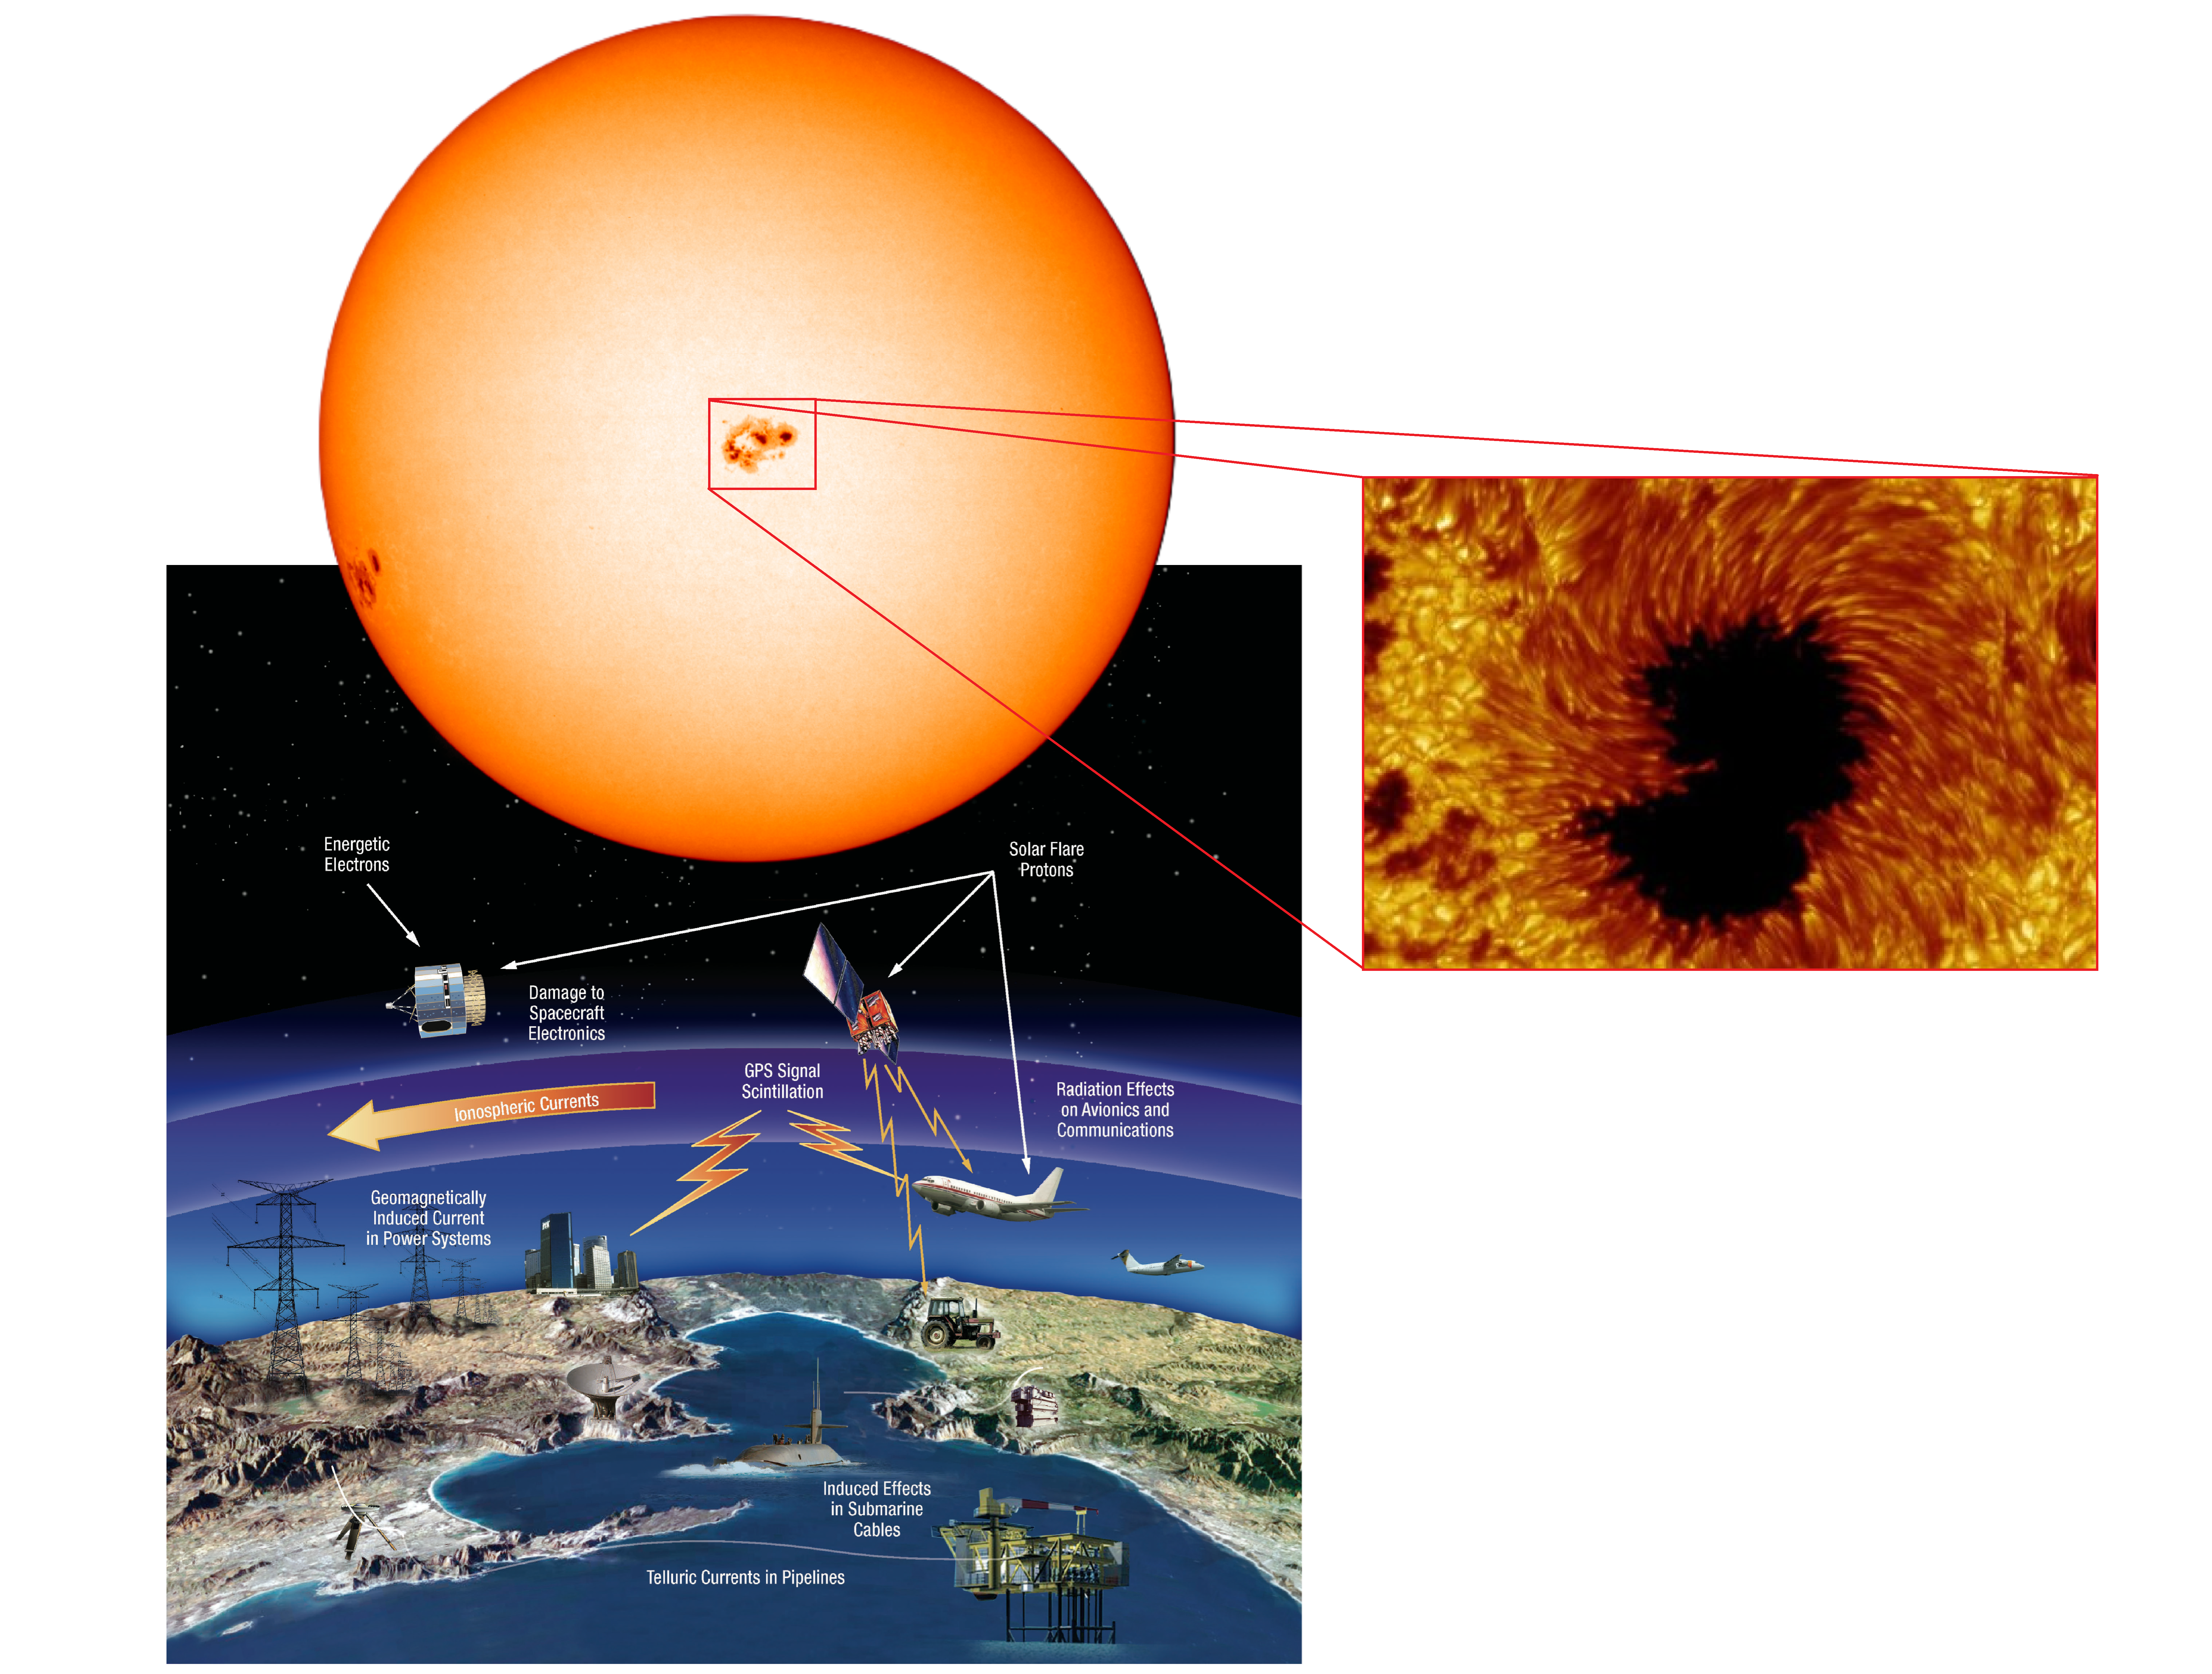
\includegraphics[width=0.85\textwidth]{figures/solar/space-weather-effects.png}
\caption{Diagrama de los principales efectos del clima espacial sobre sistemas tecnológicos y el entorno terrestre (NASA SVS). \textbf{Fuente:} NASA Scientific Visualization Studio.}
\label{fig:}
\end{figure}

La influencia de estos eventos sobre la Tierra sigue una secuencia física bien establecida. Las fulguraciones solares emiten radiación electromagnética a lo largo de un amplio espectro de frecuencias que alcanza la Tierra aproximadamente ocho minutos después de su emisión, produciendo alteraciones en la ionosfera. Por su parte, las CME expulsan grandes cantidades de plasma magnetizado al medio interplanetario. Cuando estas estructuras interactúan con la magnetosfera terrestre, pueden transferir energía, masa y momento al sistema magnetosférico mediante procesos de reconexión magnética, particularmente cuando la orientación del campo magnético interplanetario favorece el acoplamiento con el campo geomagnético terrestre \citep{spaceaustralia2026}. Como resultado, se desencadenan procesos de aceleración y transporte de partículas energéticas a lo largo de las líneas de campo magnético \citep{reyes2021geomagnetic}.

La energía inyectada durante estos procesos puede dar lugar a tormentas geomagnéticas cuyos efectos se manifiestan sobre diversos sistemas tecnológicos críticos:

\begin{itemize}
\item \textbf{Expansión atmosférica y aumento del arrastre satelital:} La deposición de energía en la termosfera incrementa su temperatura y provoca una expansión de las capas atmosféricas superiores. Como consecuencia, aumenta la densidad atmosférica a altitudes orbitales bajas, incrementando el arrastre atmosférico sobre satélites artificiales y modificando sus parámetros orbitales \citep{spaceaustralia2026}.

\item \textbf{Degradación de sistemas de telecomunicación y posicionamiento:} Las perturbaciones ionosféricas alteran la propagación de ondas de radio, ocasionando interrupciones en enlaces de alta frecuencia e introduciendo errores de retardo y fase en señales de navegación satelital, afectando la precisión de sistemas GPS y GNSS \citep{spaceaustralia2026,grodji2021study}.

\item \textbf{Corrientes inducidas geomagnéticamente (GIC):} Las variaciones temporales del campo geomagnético inducen campos eléctricos sobre la superficie terrestre, generando corrientes en infraestructuras conductoras extensas, como redes eléctricas de transmisión. Estas corrientes pueden provocar saturación parcial de transformadores y comprometer la estabilidad operativa de los sistemas de potencia \citep{spaceaustralia2026}.

\end{itemize}

Bajo este escenario, el monitoreo continuo de las manchas solares trasciende el interés puramente observacional. El número de manchas solares (\textit{Sunspot Number}, SSN) constituye uno de los indicadores indirectos más utilizados de la actividad magnética global del Sol, mientras que la morfología y evolución de las regiones activas proporcionan información relevante sobre el potencial eruptivo de la atmósfera solar.

\begin{figure}[H]
\centering
\begin{subfigure}[t]{0.31\textwidth}
\centering
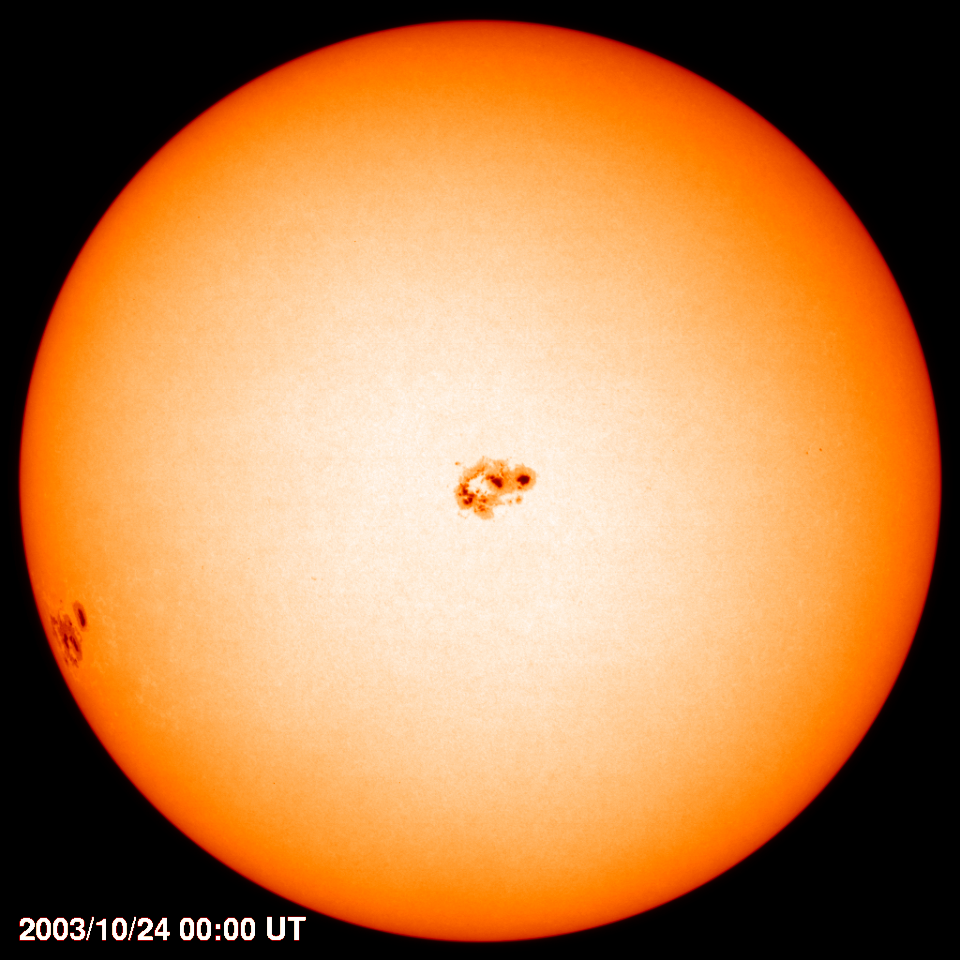
\includegraphics[width=\textwidth]{figures/solar/sunspot.png}
\caption{Imagen del disco solar completo.}
\end{subfigure}
\hfill
\begin{subfigure}[t]{0.44\textwidth}
\centering
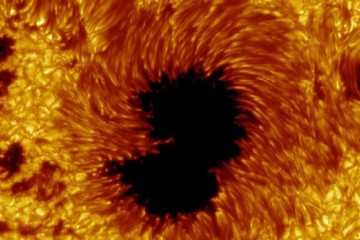
\includegraphics[width=\textwidth]{figures/solar/spot_close.jpg}
\caption{Detalles ampliados de una mancha solar.}
\end{subfigure}
\caption{Caracterización multiescala de la actividad solar: (a) disco solar completo con grupos activos fotosféricos; (b) detalle estructural de una mancha solar individual. \textbf{Fuente:} Solar Dynamics Observatory (SDO/NASA).}
\label{fig:teoria-sunspot}
\end{figure}

El estudio automatizado de estas estructuras fotosféricas permite relacionar características observacionales de las regiones activas con la probabilidad de ocurrencia de fenómenos eruptivos, incluyendo fulguraciones y eyecciones de masa coronal potencialmente geoefectivas. Esta capacidad resulta fundamental para el desarrollo de sistemas de monitoreo y modelos predictivos orientados a la caracterización del clima espacial.

\subsection{Herramientas observacionales y modalidades de observación}

La fotosfera es la capa visible del Sol y corresponde a la región desde la cual se emite la mayor parte de la radiación observada en continuo visible. En ella se reconocen estructuras como la granulación, la umbra y la penumbra de las manchas solares, por lo que constituye la referencia principal para la observación en luz blanca.

\begin{figure}[H]
  \centering
  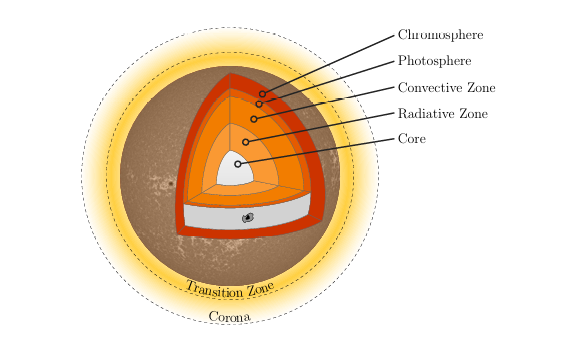
\includegraphics[width=0.76\textwidth]{figures/solar/sun_parts.png}
  \caption{Esquema general de las principales capas y regiones del Sol. La figura permite ubicar la fotosfera, cromosfera y corona dentro del contexto físico de las modalidades observacionales empleadas en heliofísica. \textbf{Fuente:} Adaptado de Sayez et al..}
  \label{fig:partes-sol}
\end{figure}

Por encima de la fotosfera se encuentra la cromosfera, una capa más tenue y estructurada por la interacción entre plasma y campo magnético, donde se observan plages, filamentos y otras manifestaciones asociadas a regiones activas. En consecuencia, la fotosfera se estudia habitualmente mediante luz blanca o continuo visible, mientras que la cromosfera suele analizarse a través de líneas espectrales como CaII K y H$\alpha$. 

Estas modalidades no son equivalentes ni redundantes. La luz blanca enfatiza umbra, penumbra y estructura fotosférica; CaII K revela plages asociadas a concentraciones de campo magnético; y H$\alpha$ muestra estructuras cromosféricas ligadas a la interacción plasma--campo.

\begin{figure}[H]
  \centering
  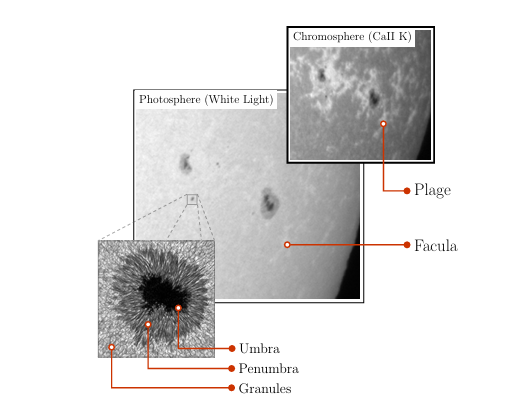
\includegraphics[width=0.82\textwidth]{figures/solar/wl_cak.png}
  \caption{Comparación observacional entre imágenes solares en luz blanca y CaII K. La figura ilustra cómo cada modalidad resalta estructuras distintas de la actividad solar. \textbf{Fuente:} Adaptado de Sayez et al..}
  \label{fig:wl-vs-caiik}
\end{figure}

Esta distinción resulta importante porque sitúa la clasificación de manchas solares dentro de un marco observacional más amplio. Aunque la presente tesis se enfoca principalmente en imágenes heliográficas de luz blanca, la interpretación física y observacional de dichas imágenes se beneficia del hecho de que forman parte de un ecosistema multibanda donde diferentes instrumentos revelan distintas capas y manifestaciones de la actividad solar \citep{scherrer2012hmi,bobra2014sharp}.

\subsection{Observatorios terrestres y elementos atmosféricos}

Las observaciones terrestres muestran que el monitoreo solar comenzó con proyecciones telescópicas y dibujos, y que evolucionó hacia observatorios equipados con telescopios ópticos, sensores digitales y, en algunos casos, arreglos distribuidos para observación sinótica. Dentro de esta categoría se mencionan, entre otros, redes globales como GONG y estaciones solares de larga duración como el Uccle Solar Equatorial Table (USET) del Observatorio Real de Bélgica. Estos sistemas son relevantes porque combinan seguimiento instrumental del Sol, continuidad temporal de registros y disponibilidad de productos útiles para contrastar procedimientos de análisis automático \citep{nsoGONG2026,robUSET2026,sidcGroundObservations2026}.

En el caso de USET, la referencia es principalmente metodológica e histórica. La estación opera una mesa ecuatorial con telescopios dedicados a observaciones en luz blanca, H$\alpha$ y CaII K, además de una tradición prolongada de dibujos solares y catálogos derivados. Por ello, USET permite ilustrar cómo un observatorio terrestre puede integrar adquisición digital, observación visual, anotación humana y preservación de metadatos dentro de una misma cadena observacional \citep{robUSET2026,sidcGroundObservations2026}.

\begin{figure}[H]
  \centering
  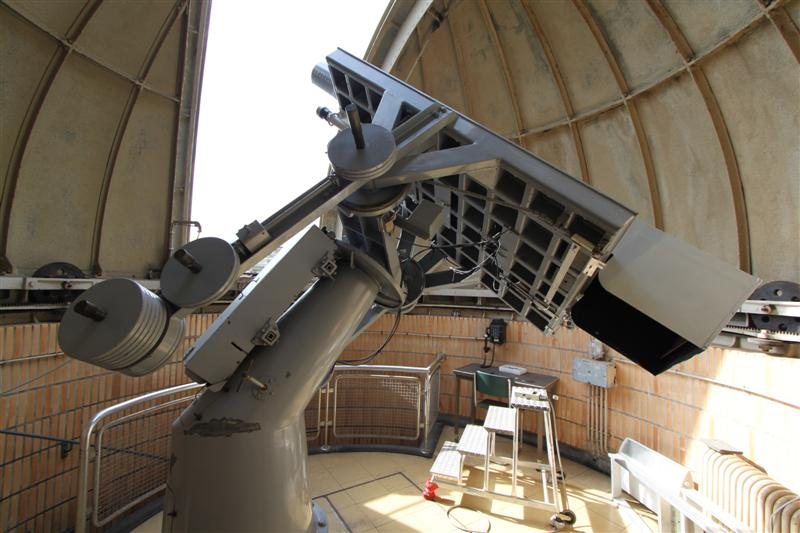
\includegraphics[width=0.78\textwidth]{figures/solar/scope_proj.jpg}
  \caption{Instalación instrumental del Uccle Solar Equatorial Table (USET), empleada para el seguimiento terrestre sistemático del Sol en distintas modalidades observacionales. \textbf{Fuente:} página oficial del Observatorio Real de Bélgica.}
  \label{fig:uset-instrument}
\end{figure}

A diferencia de esa referencia internacional, el contexto operativo directo de esta tesis se atribuye al Observatorio Astronómico ``Prof. Alexis Troche Boggino'', espacio académico de observación, formación y apoyo a actividades astronómicas asociado a la Facultad Politécnica de la Universidad Nacional de Asunción. Este entorno proporciona la referencia institucional y práctica para el desarrollo del prototipo, ya que permite vincular la adquisición de imágenes solares con una infraestructura real de observación, supervisión y registro.

La Figura~\ref{fig:observatorio-alexis-troche} muestra dicho contexto local. La subfigura (a) corresponde a la sala de control del Observatorio Astronómico ``Prof. Alexis Troche Boggino'', desde donde se supervisan actividades instrumentales y de observación; la subfigura (b) presenta el telescopio principal del observatorio. Aunque esta infraestructura principal define el entorno institucional y observacional del trabajo, para el desarrollo del prototipo se considera el uso de un telescopio refractor Vixen con diámetro $D=60\,\mathrm{mm}$ y distancia focal $F=420\,\mathrm{mm}$ como plataforma óptica de prueba, lo que permite trabajar con una configuración más compacta, segura y controlable durante las etapas de integración de cámara, filtrado solar, preprocesamiento local y validación inicial.

\begin{figure}[H]
    \centering
    \begin{subfigure}[t]{0.65\textwidth}
        \centering
        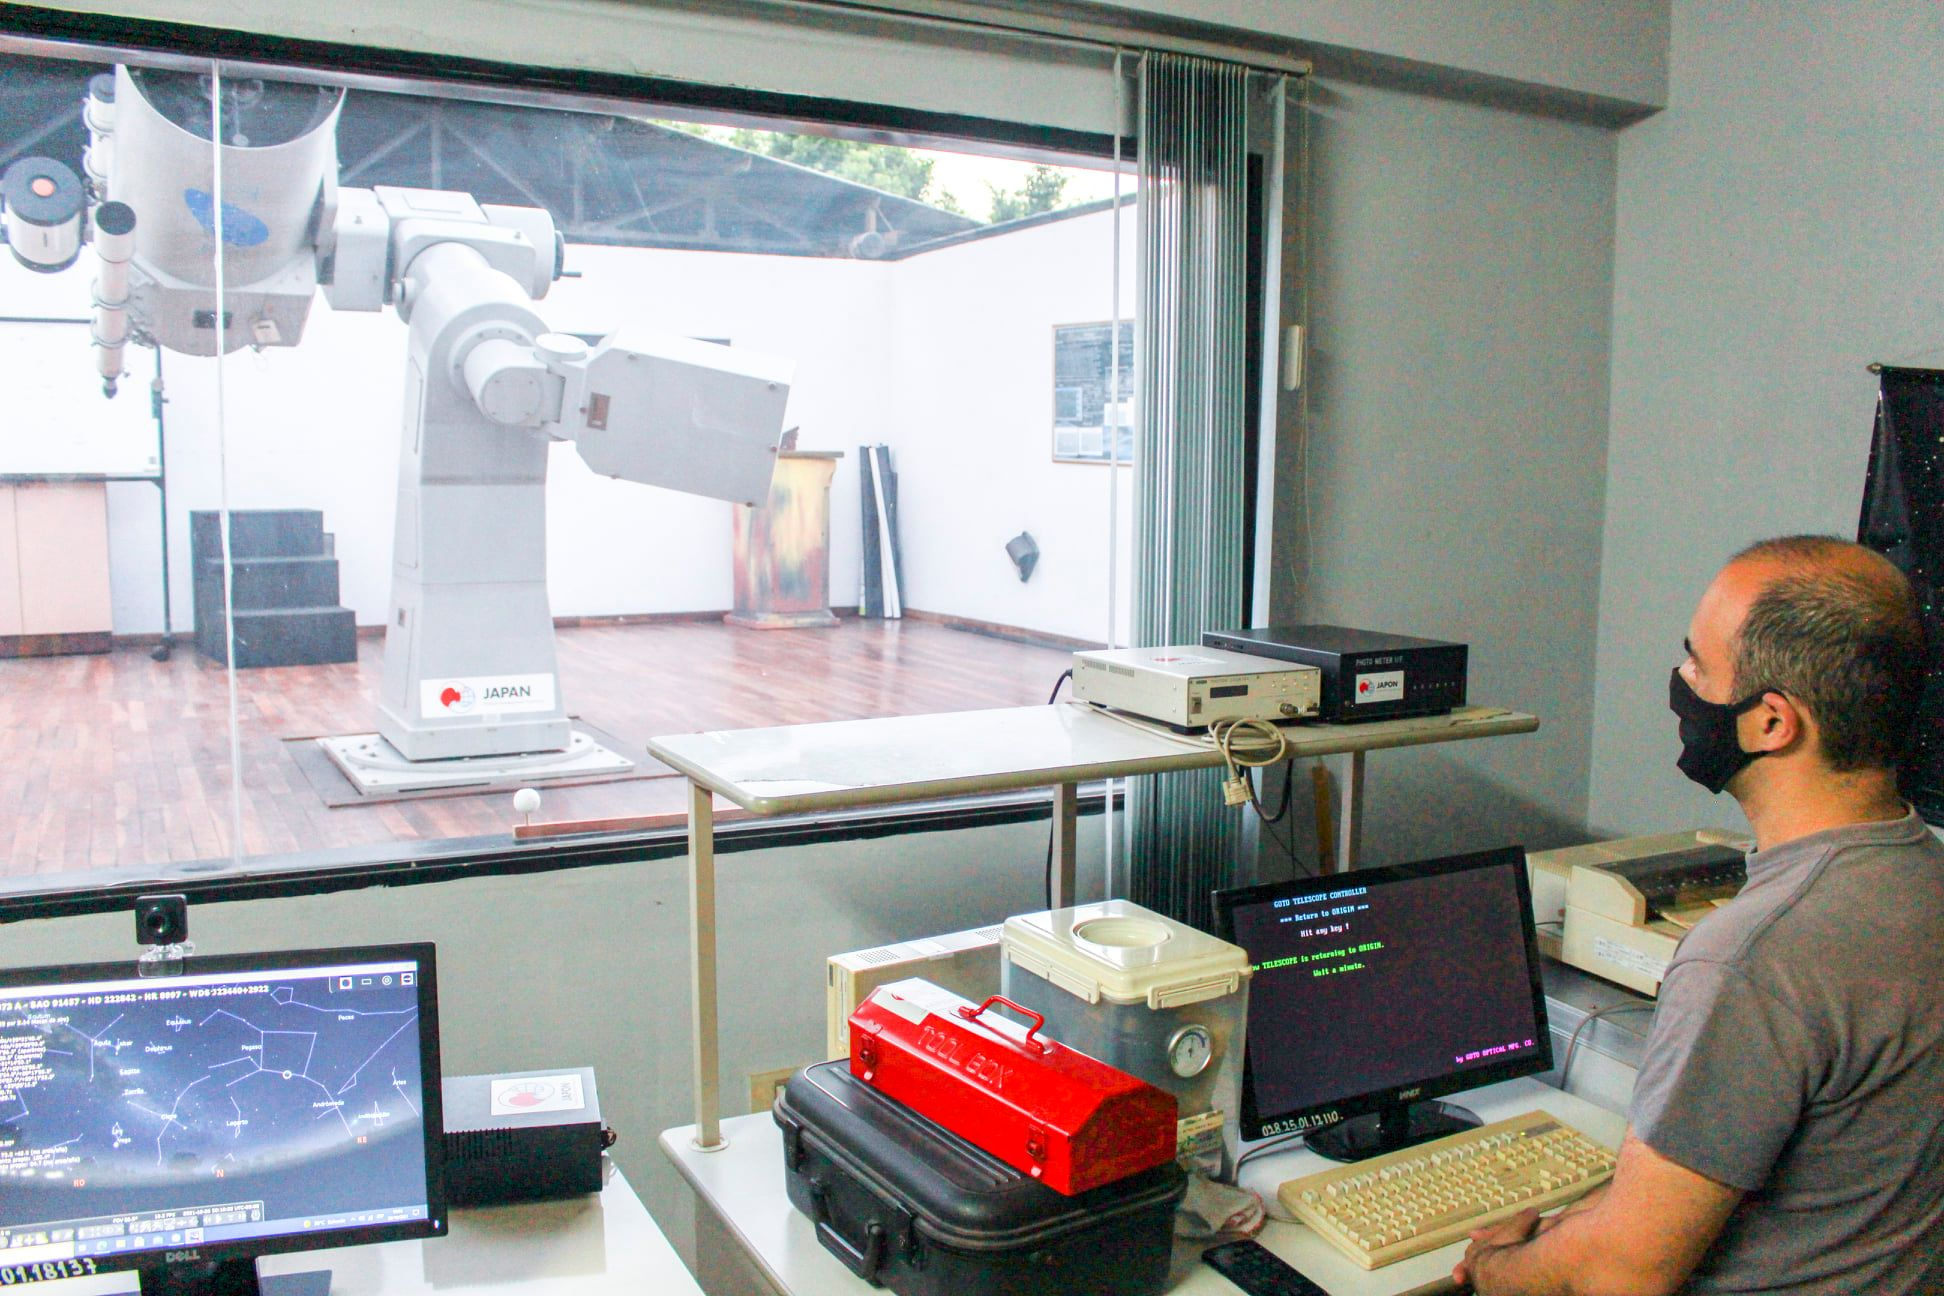
\includegraphics[width=\textwidth]{figures/obs/control.jpg}
        \caption{Sala de control del Observatorio Astronómico ``Prof. Alexis Troche Boggino''.}
    \end{subfigure}
    \hfill
    \begin{subfigure}[t]{0.30\textwidth}
        \centering
        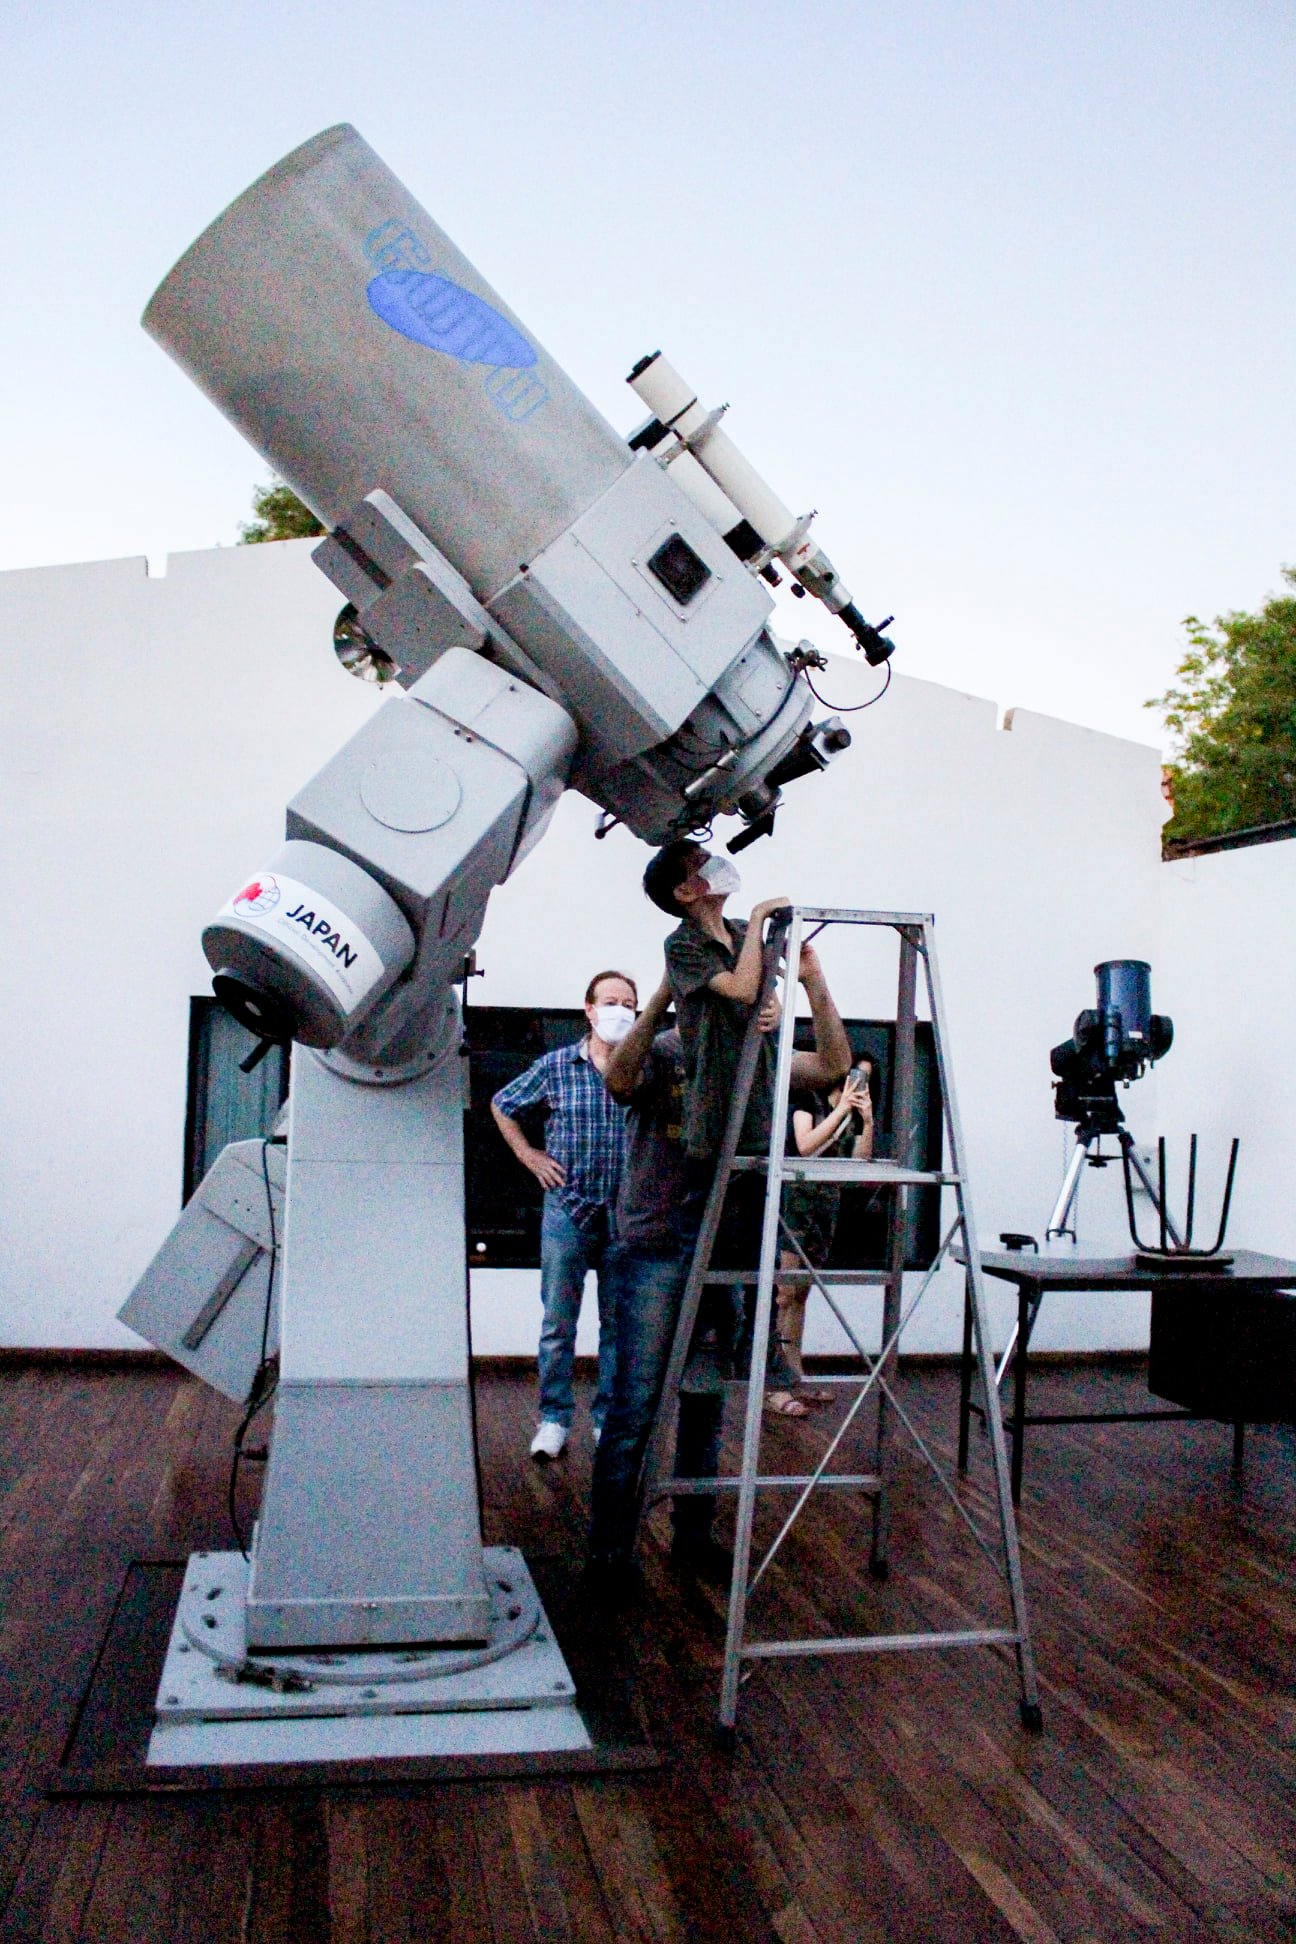
\includegraphics[width=\textwidth]{figures/obs/scope.jpg}
        \caption{Telescopio principal del observatorio.}
    \end{subfigure}
    \caption{Contexto instrumental del Observatorio Astronómico ``Prof. Alexis Troche Boggino''. La figura documenta (a) la sala de control empleada para supervisión y operación, y (b) el telescopio principal disponible en el entorno de trabajo. \textbf{Fuente:} Elaboración propia.}
    \label{fig:observatorio-alexis-troche}
\end{figure}

Las observaciones terrestres están inevitablemente afectadas por artefactos atmosféricos. Entre ellos se cuentan el \textit{seeing}, la nubosidad, el polvo sobre la óptica y la oclusión por aves o aeronaves. Estos factores producen desenfoque, distorsión y pérdidas parciales de información, y constituyen una de las principales razones por las que el análisis automático en observatorios terrestres resulta más desafiante que en imágenes espaciales. Esta observación es especialmente importante para una tesis como la presente, ya que justifica decisiones de preprocesamiento, selección de cuadros e incluso de diseño de modelos robustos frente a degradaciones no ideales.

\subsection{Observatorios espaciales y complementariedad instrumental}

La discusión de observatorios terrestres se complementa con la de observatorios espaciales. Las misiones en espacio permiten superar limitaciones atmosféricas y acceder a observaciones continuas, multiespectrales y de alta estabilidad. Entre las plataformas destacadas se encuentran SDO, SOHO, IRIS y STEREO. Estas misiones incorporan sensores capaces de observar el Sol en visible, EUV y otras longitudes de onda, así como de producir magnetogramas y reconstrucciones del campo magnético solar \citep{scherrer2012hmi,bobra2014sharp}.

\begin{figure}[H]
  \centering
  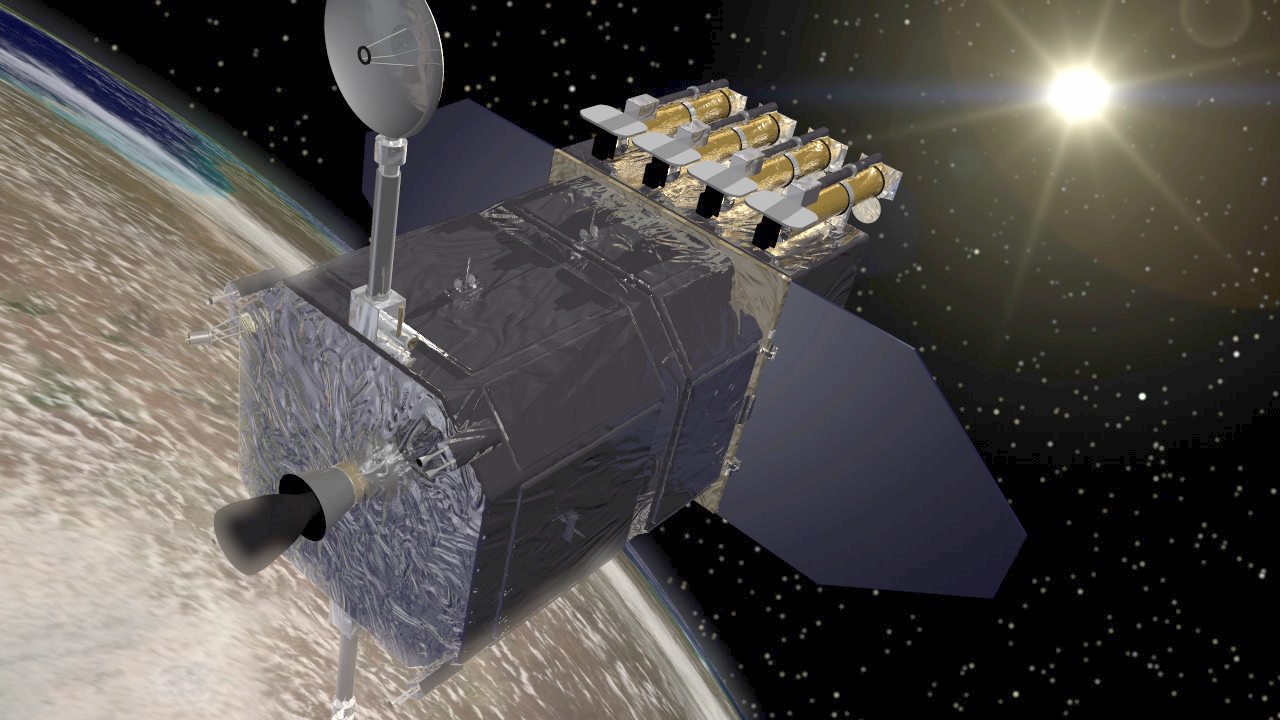
\includegraphics[width=0.78\textwidth]{figures/obs/sdo.jpg}
  \caption{Representación artística de la nave Solar Dynamics Observatory (SDO) desplegada en órbita. \textbf{Fuente:} NASA, \textit{Artist's rendition of the deployed SDO spacecraft}.}
  \label{fig:sdo-spacecraft}
\end{figure}

Para esta tesis, la importancia de tales observatorios no radica solamente en su valor científico intrínseco, sino también en su papel para la adquisición de bases de datos para entrenamiento, validación y contraste. La integración entre observaciones terrestres y espaciales amplía la capacidad de modelado del sistema solar atmosférico y habilita enfoques híbridos en los que catálogos, imágenes sinóticas y productos derivados se complementan entre sí.

\subsection{Clasificaciones observacionales de regiones activas}

La descripción de manchas solares se completa con las taxonomías empleadas para representar la complejidad de los grupos observados. En la práctica solar conviven dos familias de clasificación particularmente relevantes. Por un lado, la clasificación magnética de Mount Wilson describe la distribución de polaridad en una región activa \citep{hale1919magneticpolarity,noaaSRS} y se expresa operativamente en categorías como $\alpha$, $\beta$, $\gamma$, $\beta\gamma$ y sus variantes con modificador $\delta$. Esta taxonomía es especialmente útil cuando interesa relacionar complejidad magnética y potencial eruptivo \citep{noaaSRS}.

\begin{figure}[H]
  \centering
  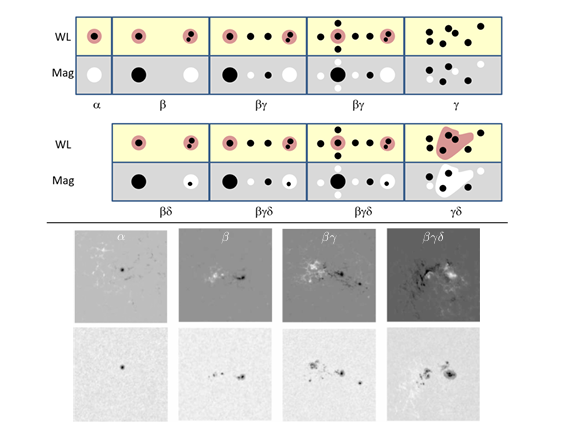
\includegraphics[width=0.65\textwidth]{figures/solar/wilson.png}
  \caption{Esquema ilustrativo de la clasificación magnética de Mount Wilson para regiones activas. La figura resume la organización de polaridades magnéticas empleada para diferenciar configuraciones simples, bipolares y complejas. \textbf{Fuente:} Adaptado de Sayez et al..}
  \label{fig:wilson-classification}
\end{figure}

Por otro lado, para observación en luz blanca y para el análisis fino de la geometría fotosférica, la clasificación Zurich--McIntosh ofrece una descripción más rica porque no se limita a indicar la polaridad magnética, sino que codifica la apariencia visible del grupo solar.

\begin{figure}[H]
  \centering
  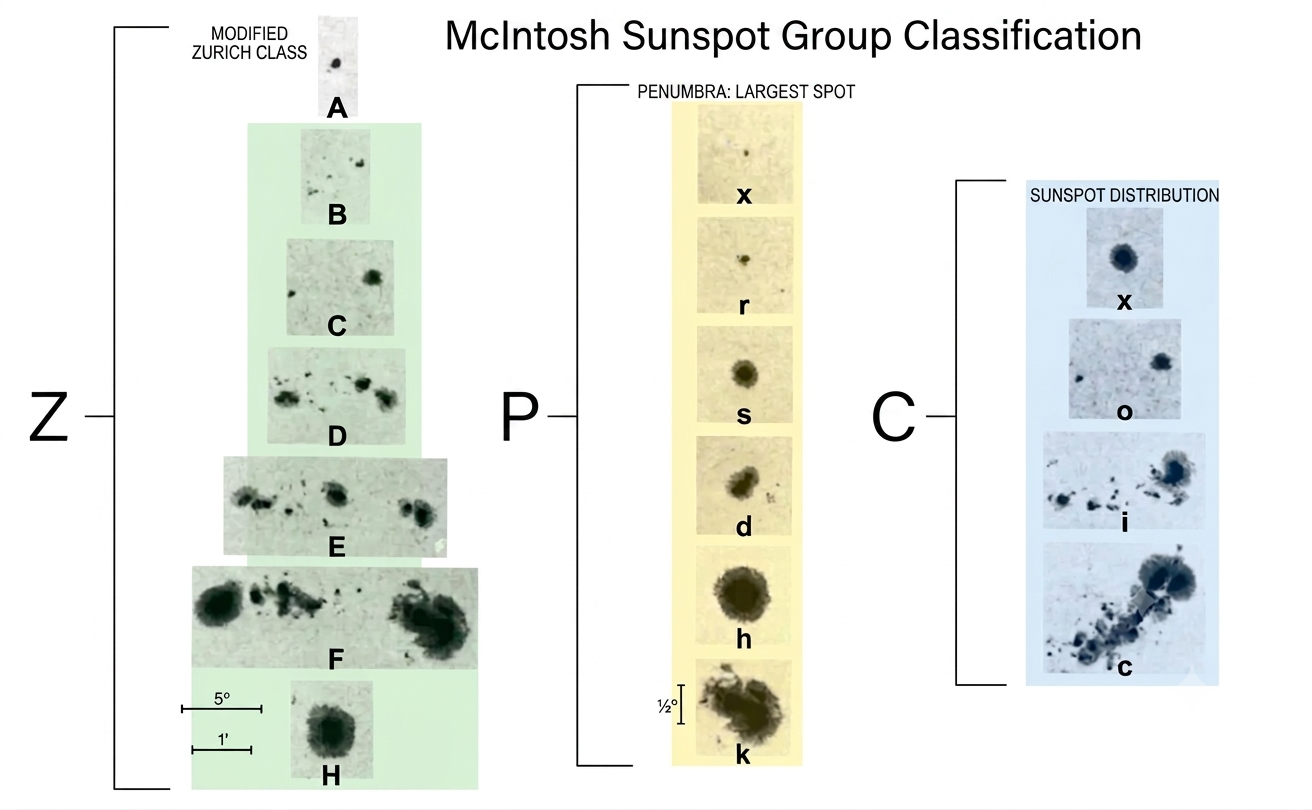
\includegraphics[width=0.62\textwidth]{figures/solar/mcintosh.png}
  \caption{Esquema general de la clasificación de McIntosh. La figura resume la combinación jerárquica de la clase Zurich, el tipo penumbral y la compactación interna del grupo solar. \textbf{Fuente:} Courtesy Patrick S. McIntosh, NOAA (1990).}
  \label{fig:mcintosh-scheme}
\end{figure}

Formalmente, estas componentes se denotan como $Z$, que describe la organización global del grupo; $P$, que caracteriza el tipo penumbral dominante; y $C$, que representa el grado de compactación interna. Esta estructura jerárquica no es solo una convención catalográfica, sino una forma compacta de codificar estado observacional, evolución estructural y relaciones geométricas visibles sobre el disco solar \citep{mcintosh1990classification,bornmann1994flarerates}.

Desde el punto de vista de esta tesis, la importancia de Zurich--McIntosh radica en que preserva semántica observacional y, al mismo tiempo, puede formularse como un problema apto para inferencia automática. Aunque la taxonomía completa puede expresarse como 60 combinaciones operativas, su interés principal no está en la enumeración exhaustiva de etiquetas, sino en la lógica jerárquica que conecta morfología global, penumbra y compactación. Precisamente por ello resulta una base adecuada para modelos de clasificación estructurada \citep{mcintosh1990classification,zhou2023mcintosh,deng2025mcintosh}.

\subsection{Cámaras para observación solar}

La discusión instrumental debe descender desde el nivel del observatorio hasta el nivel de los sensores concretos. Las cámaras constituyen el elemento que transforma la radiación proveniente del Sol en una señal digital utilizable por algoritmos de procesamiento, y por ello condicionan de manera directa la resolución espacial, la profundidad radiométrica, la cadencia temporal y la estabilidad global de la observación. En el caso de Observatorios como el USET, puede reconocerse una transición desde una práctica histórica basada en observación visual y dibujos a adquisición digital sostenida por cámaras CCD y actualmente a cámaras CMOS. Esta evolución muestra que el cambio de sensor no solo mejora la operatividad del sistema, sino que redefine la calidad y la naturaleza de los datos disponibles para el análisis.

Desde el punto de vista tecnológico, la distinción clásica entre CCD y CMOS sigue siendo importante para comprender la evolución reciente de la instrumentación astronómica. En un CCD, la carga fotoeléctrica generada en los píxeles se transfiere de manera secuencial hacia un número reducido de nodos de lectura, donde finalmente se convierte en voltaje. Esta arquitectura favoreció durante mucho tiempo una excelente uniformidad de lectura y una reputación de alta calidad científica, pero también conlleva mayor complejidad de transferencia de carga, mayor consumo energético y, en general, menores velocidades de lectura. En un CMOS, por el contrario, la conversión carga--voltaje se realiza localmente en cada píxel o en regiones muy próximas a él, lo que permite lecturas más rápidas, diseños más compactos y menor demanda energética \citep{janesick2001scientific,fossum1997cmos,zwoASI174Manual2025}.

\begin{figure}[H]
    \centering
    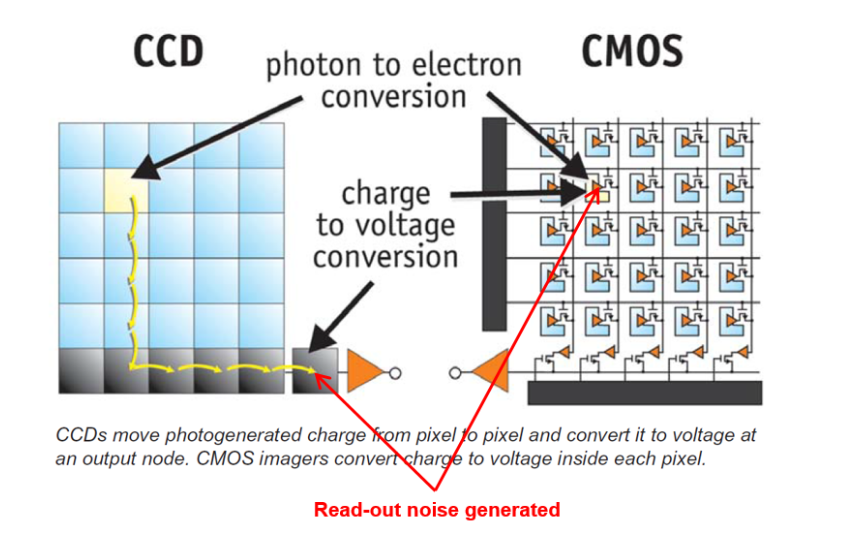
\includegraphics[width=0.78\textwidth]{figures/ml/yolo_label.png}
    \caption{Esquema conceptual de lectura en sensores CCD y CMOS. En el CCD, la carga fotoeléctrica se desplaza píxel a píxel hasta un nodo común de salida, mientras que en el CMOS la conversión carga--voltaje ocurre de forma local en cada píxel o en su vecindad inmediata. \textbf{Fuente:} Adaptado de Stefano Meroli, CERN.}
    \label{fig:ccd-cmos-readout}
\end{figure}

La diferencia entre ambas arquitecturas también tiene implicancias observacionales concretas. La literatura sobre sensores científicos indica que, en sensores CCD, el \textit{binning} puede mejorar de manera muy significativa la relación señal--ruido cuando varias cargas se suman antes de una única lectura, mientras que en CMOS el beneficio no escala de la misma manera porque el ruido de lectura se aplica a cada píxel durante la conversión local \citep{janesick2001scientific,fossum1997cmos}. Del mismo modo, la literatura técnica destaca que los CCD pueden presentar \textit{blooming} cuando una sobrecarga en un píxel se derrama hacia registros vecinos, mientras que los CMOS son intrínsecamente menos susceptibles a este fenómeno al evitar registros extensos de transferencia de carga \citep{janesick2001scientific,fossum1997cmos}. Estas diferencias no implican que una tecnología sea universalmente superior a la otra, pero sí explican por qué cada arquitectura ofrece ventajas distintas según el régimen de observación.

En astrofotografía y observación solar contemporánea, la tendencia general se ha desplazado de forma marcada hacia sensores CMOS. Esta transición se explica por la combinación de menor costo de fabricación, menor consumo, altas tasas de cuadro, ruido de lectura cada vez más competitivo y una mejora sostenida de la sensibilidad cuántica. Incluso en ámbitos donde durante años los CCD dominaron por su calidad científica, la brecha de desempeño se ha reducido de manera sustancial, y en múltiples aplicaciones los CMOS actuales ya igualan o superan prestaciones tradicionalmente asociadas a CCD astronómicos \citep{janesick2001scientific,fossum1997cmos}. Para sistemas locales de observación solar, donde interesan portabilidad, cadencia elevada y facilidad de integración con procesamiento en tiempo real, esta tendencia resulta especialmente relevante.


\begin{figure}[H]
    \centering
    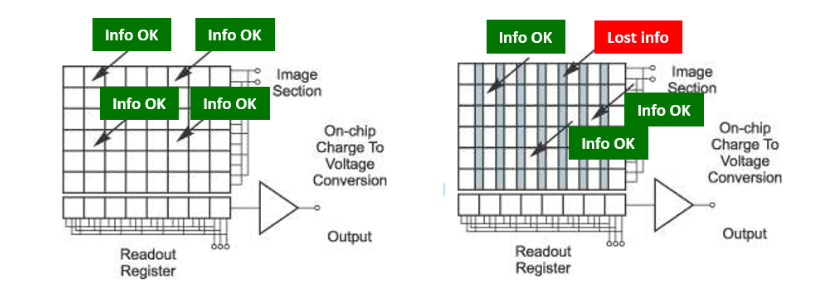
\includegraphics[width=0.86\textwidth]{figures/ml/yolo_box.png}
    \caption{Esquema conceptual del efecto de lectura sobre la integridad de la información en sensores con conversión distribuida. \textbf{Fuente:} Adaptado de Stefano Meroli, CERN.}
    \label{fig:ccd-cmos-info}
\end{figure}

Las Figuras \ref{fig:ccd-cmos-readout} y \ref{fig:ccd-cmos-info} resumen visualmente esta diferencia de arquitectura. La primera destaca el contraste entre transferencia serial de carga en CCD y conversión local en CMOS, mientras que la segunda ayuda a interpretar por qué la organización del trayecto de lectura puede impactar la preservación de información útil y la generación de ruido durante la adquisición.

\section{Estado del Arte}

En esta tesis, el estado del arte se organiza a partir de una limitación observada en el ecosistema tecnológico disponible: existen soluciones comerciales avanzadas para asistir la adquisición y operación de equipos de astrofotografía, así como investigaciones recientes para detectar, agrupar, clasificar y predecir la actividad asociada a manchas solares; sin embargo, no se identifican ecosistemas comerciales de observación astrofotográfica que integren de forma específica todas las etapas requeridas para este trabajo, desde la adquisición local de imágenes solares hasta el análisis morfológico y la generación de indicadores predictivos basados en modelos computacionales. Por ello, la revisión se presenta en subsecciones complementarias que cubren, primero, dispositivos comerciales de adquisición asistida y, luego, contribuciones recientes sobre análisis automático de manchas solares.

En el plano algorítmico, el problema automático de análisis de manchas solares se organiza en dos ejes complementarios: el agrupamiento y clasificación morfológica, y el análisis predictivo de la actividad de manchas solares (Número de manchas solares y distribución latitudinal). Esta descomposición no es arbitraria, sino que responde a la propia lógica observacional del problema. La clasificación Zurich--McIntosh se aplica sobre el grupo solar como unidad de análisis y no sobre manchas aisladas; por ello, antes de clasificar, es necesario detectar y asociar correctamente las manchas que pertenecen a una misma estructura activa \citep{sayez2023sunscc}. De forma complementaria, la interpretación temporal de esos grupos se inserta en la modulación de gran escala impuesta por el ciclo solar.

\subsection{Dispositivos comerciales de adquisición de imágenes asistida}

Los dispositivos comerciales de adquisición asistida para astrofotografía han evolucionado hacia unidades compactas que combinan control de cámaras, monturas, enfocadores, ruedas portafiltros, alimentación eléctrica y conectividad inalámbrica. Su objetivo principal es reducir la complejidad operativa de una sesión de captura, centralizando el control instrumental en una aplicación móvil o en una interfaz remota. La Figura~\ref{fig:hw-art-state-commercial} muestra tres ejemplos representativos de esta tendencia: ZWO ASIAIR, PrimaLuceLab EAGLE6 y StellarMate Pro.

\begin{figure}[H]
    \centering
    \begin{subfigure}[t]{0.31\textwidth}
        \centering
        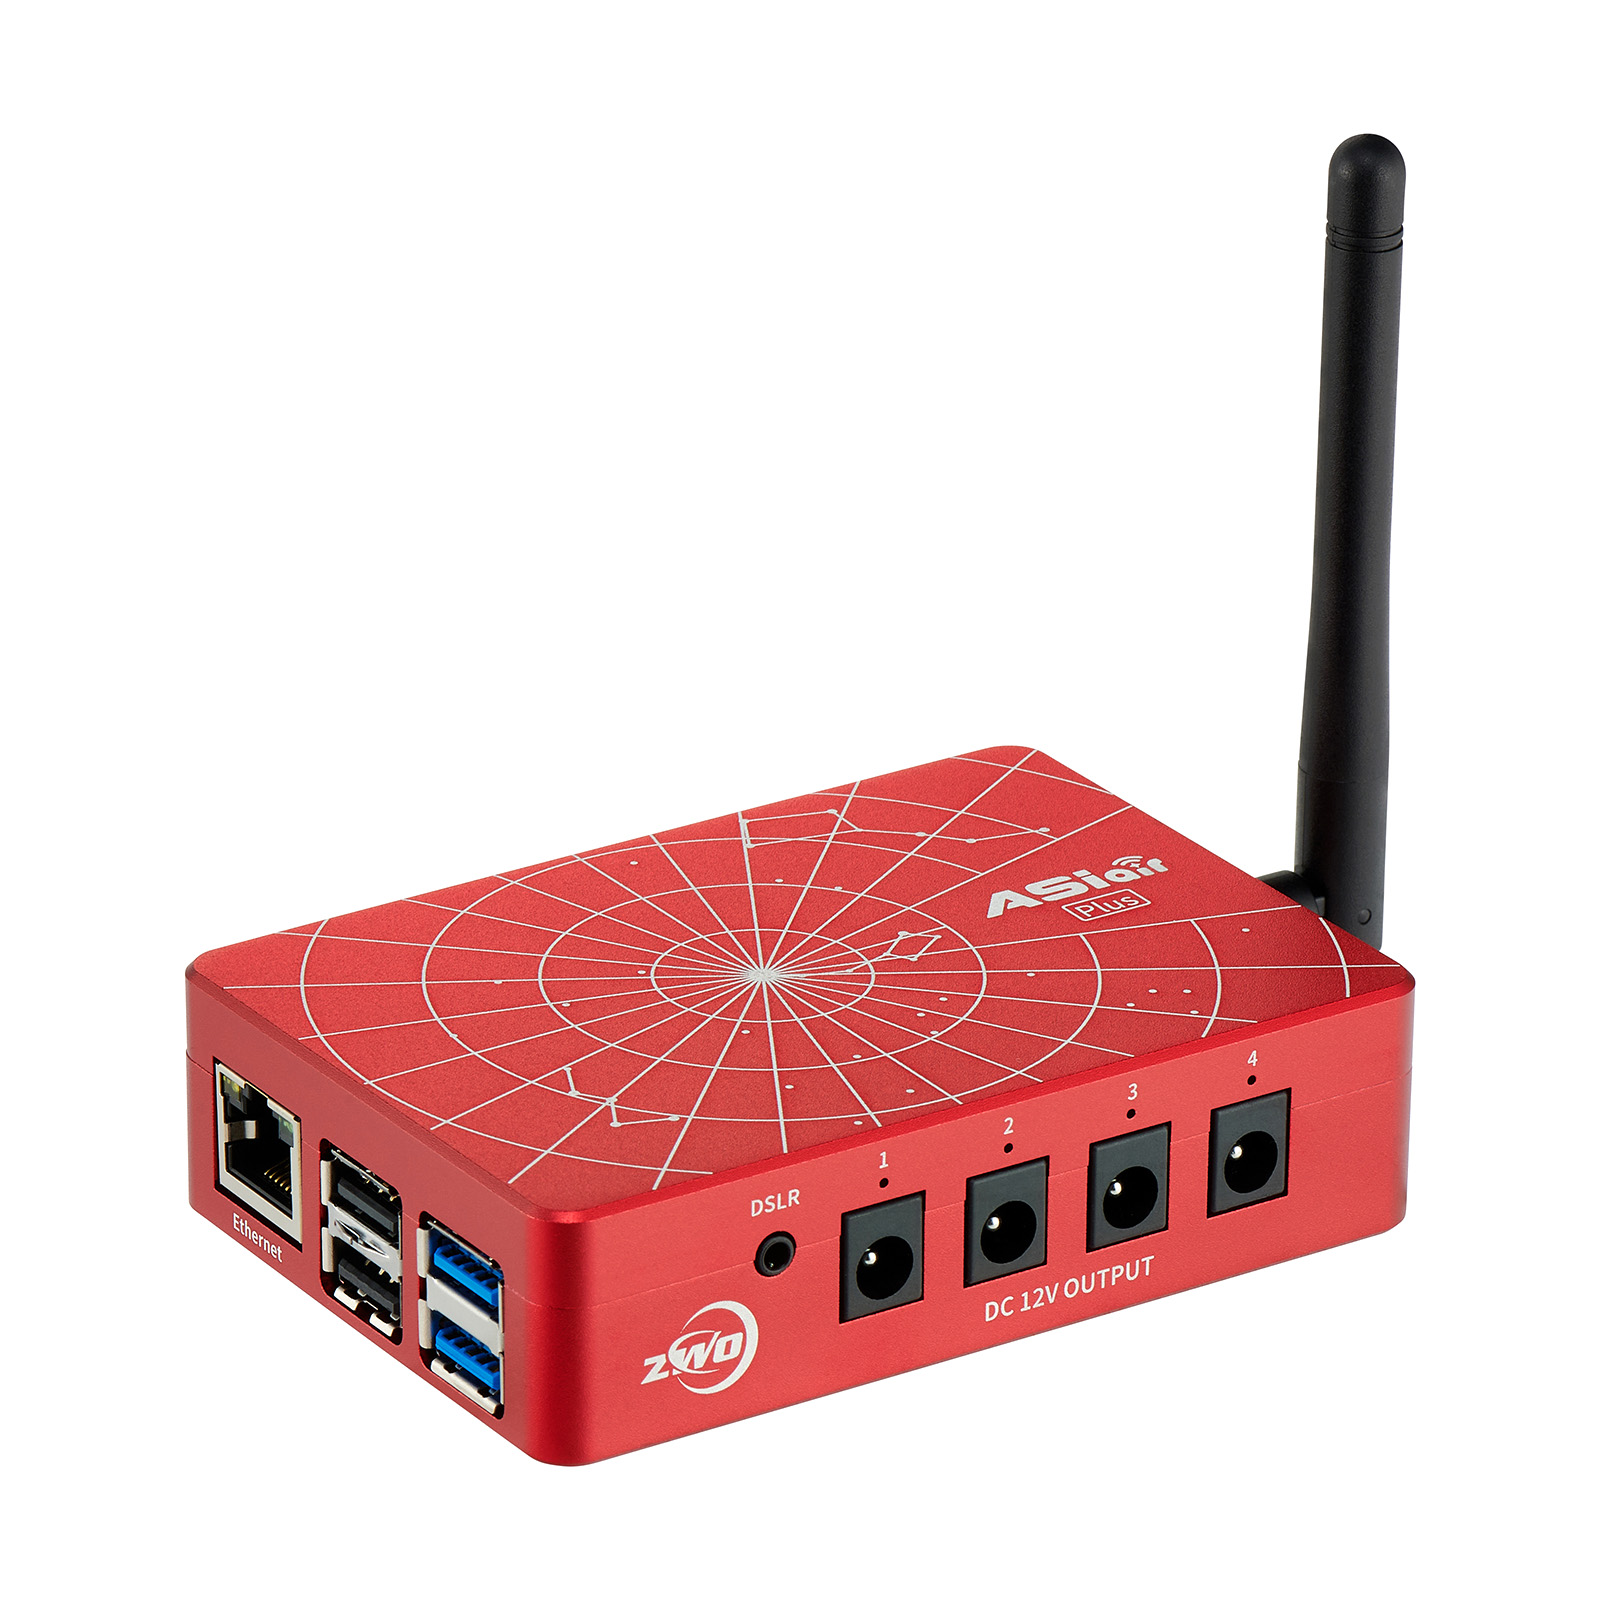
\includegraphics[width=\textwidth]{figures/hw_art_state/zwo_asiair.jpg}
        \caption{ZWO ASIAIR.}
    \end{subfigure}
    \hfill
    \begin{subfigure}[t]{0.31\textwidth}
        \centering
        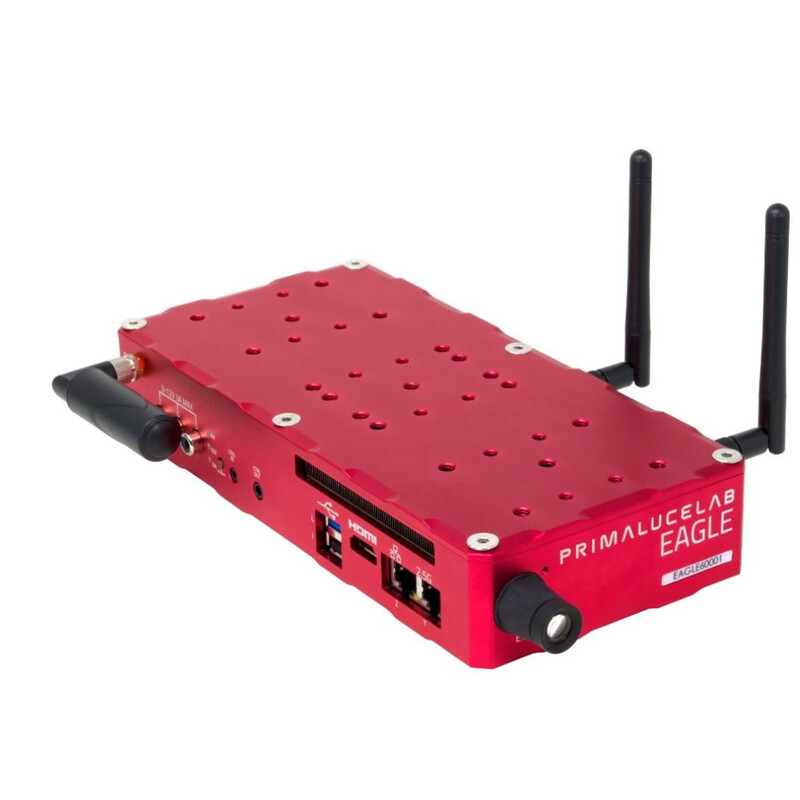
\includegraphics[width=\textwidth]{figures/hw_art_state/primaLuceLab-Eagle6.jpg}
        \caption{PrimaLuceLab EAGLE6.}
    \end{subfigure}
    \hfill
    \begin{subfigure}[t]{0.31\textwidth}
        \centering
        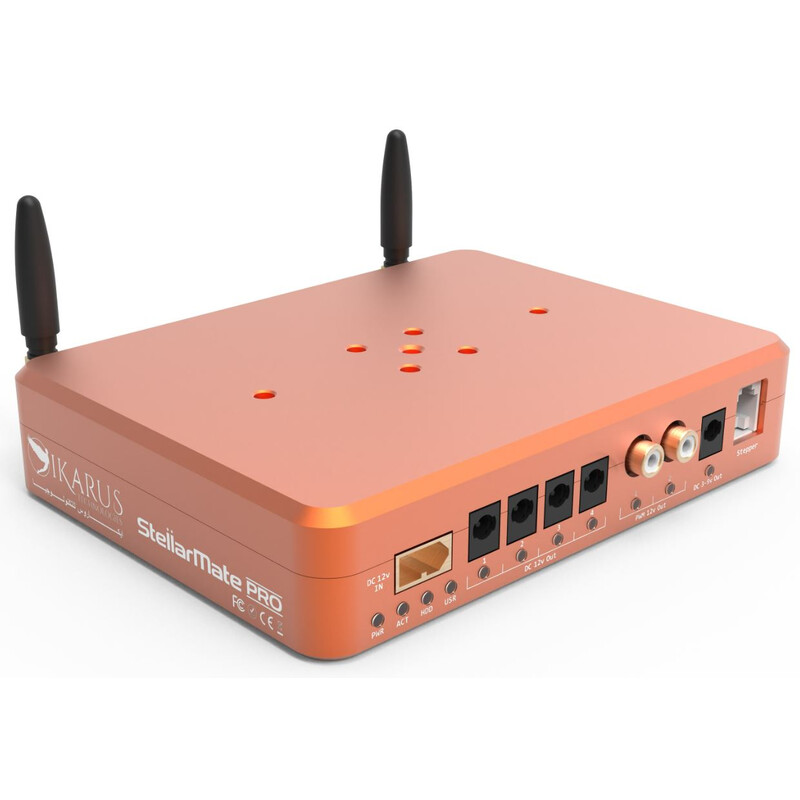
\includegraphics[width=\textwidth]{figures/hw_art_state/stellar_mate-pro-8GB-128GB.jpg}
        \caption{StellarMate Pro.}
    \end{subfigure}
    \caption{Dispositivos comerciales de adquisición asistida empleados como referencia del estado del arte instrumental en astrofotografía. \textbf{Fuente:} páginas oficiales de ZWO, PrimaLuceLab y StellarMate.}
    \label{fig:hw-art-state-commercial}
\end{figure}

ZWO ASIAIR representa una aproximación cerrada y altamente integrada alrededor del ecosistema ZWO. En su versión Plus de 256~GB se comercializa alrededor de US\$349, incorpora 4~GB de RAM DDR4, almacenamiento eMMC de 32~GB o 256~GB, red Gigabit Ethernet, WiFi de doble banda y cuatro salidas de 12~V con capacidad máxima conjunta de 5~A \citep{zwoASIAIR2026,bhASIairPlus2026}. Su principal fortaleza es la simplicidad de uso y la integración directa con cámaras, monturas y accesorios compatibles, aunque dicha integración tiende a privilegiar un entorno de hardware específico.

PrimaLuceLab EAGLE6 adopta una estrategia más cercana a una computadora industrial para telescopios. Su precio de referencia es aproximadamente US\$1595 e integra Windows 11 Enterprise, procesador Intel Celeron J6412, 8~GB de memoria DDR4, almacenamiento NVMe industrial de 128~GB, conectividad WiFi 6E, GPS, diez puertos USB y siete salidas de alimentación de 12~V, además de sensores auxiliares para monitoreo de cielo, inclinación y movimiento \citep{primaluceEagle62026,primaluceEagle6USA2026}. Por estas características, se orienta a configuraciones de observatorio o montajes de mayor complejidad, donde la distribución de energía y la gestión remota son tan importantes como la captura de imágenes.

StellarMate Pro, por su parte, se presenta como un controlador de clase observatorio basado en tecnologías abiertas. La versión de 128~GB se ofrece alrededor de US\$599 e incorpora 8~GB de RAM, SSD de 128~GB, procesador Broadcom BCM2711, cuatro puertos USB 3.0, dos puertos USB 2.0, cuatro salidas de 12~V, dos salidas para calentadores antirocío, una salida variable de 3--9~V, conectividad HDMI/Ethernet/GPS/WiFi y sistema StellarMate OS precargado \citep{stellarmatePro2026}. A diferencia de soluciones más cerradas, su propuesta enfatiza compatibilidad con distintos fabricantes mediante el ecosistema INDI/KStars/Ekos, lo que resulta atractivo para configuraciones heterogéneas.

La Tabla~\ref{tab:dispositivos-adquisicion-comerciales} resume las características técnicas más relevantes para comparar estos dispositivos como plataformas de adquisición asistida. Los precios deben interpretarse como valores comerciales de referencia sujetos a variación por distribuidor, impuestos, disponibilidad y configuración seleccionada.

\begin{table}[H]
\centering
\caption{Exploración de dispositivos comerciales de adquisición asistida para astrofotografía. Los precios son referenciales y pueden variar según configuración, distribuidor y fecha de consulta. \textbf{Fuente:} Elaboración propia a partir de páginas oficiales y distribuidores autorizados \citep{zwoASIAIR2026,bhASIairPlus2026,primaluceEagle62026,primaluceEagle6USA2026,stellarmatePro2026}.}
\label{tab:dispositivos-adquisicion-comerciales}
\uniformtablestyle
\begin{tabularx}{\textwidth}{>{\raggedright\arraybackslash}p{3.35cm} >{\raggedright\arraybackslash}p{3.15cm} >{\centering\arraybackslash}p{1.45cm} X}
\toprule
\textbf{Fabricante / modelo} & \textbf{Característica técnica} & \textbf{Precio ref.} & \textbf{Observaciones} \\
\midrule
ZWO ASIAIR Plus 256~GB & 4~GB DDR4; 32/256~GB eMMC; Ethernet; WiFi 2.4/5~GHz & US\$349 & Se destaca por su integración directa con el ecosistema ZWO y por operar desde la aplicación ASIAIR en teléfono inteligente o tableta. \\
PrimaLuceLab EAGLE6 & 8~GB DDR4; 128~GB NVMe SSD; WiFi 6E; Ethernet 2.5~Gb; GPS; Windows 11 Enterprise & US\$1595 & Se destaca por su enfoque de computadora industrial para telescopios, con sensores auxiliares y gestión avanzada de observatorio. \\
StellarMate Pro 128~GB & 8~GB LPDDR4; 128~GB SSD; WiFi 5; Bluetooth 5.0; Ethernet; GPS; StellarMate OS & US\$599 & Se destaca por su compatibilidad con equipos heterogéneos mediante INDI/KStars/Ekos y por una propuesta basada en tecnologías abiertas. \\
\bottomrule
\end{tabularx}
\end{table}

Estos productos evidencian que el mercado ya ofrece plataformas robustas para automatizar la adquisición y operación instrumental. No obstante, su alcance se concentra principalmente en la captura astrofotográfica, el control de periféricos y el soporte a flujos de observación general. En contraste, el objetivo de esta tesis requiere integrar adquisición solar en luz blanca, preprocesamiento local, detección y agrupamiento de manchas, clasificación Zurich--McIntosh y análisis predictivo de la actividad solar dentro de un flujo específico. Esta brecha justifica revisar por separado tanto el estado del arte instrumental como los avances recientes en análisis automático de manchas solares.

\subsection{Agrupamiento y clasificación de manchas solares}

Las investigaciones recientes \cite{sayez2023sunscc} sugieren que las estrategias más consistentes no abordan el problema como una clasificación directa de regiones aisladas, sino como una arquitectura modular en la que primeramente se detectan y agrupan manchas individuales, y luego se clasifica el grupo solar resultante. 
\begin{figure}[H]
    \centering
    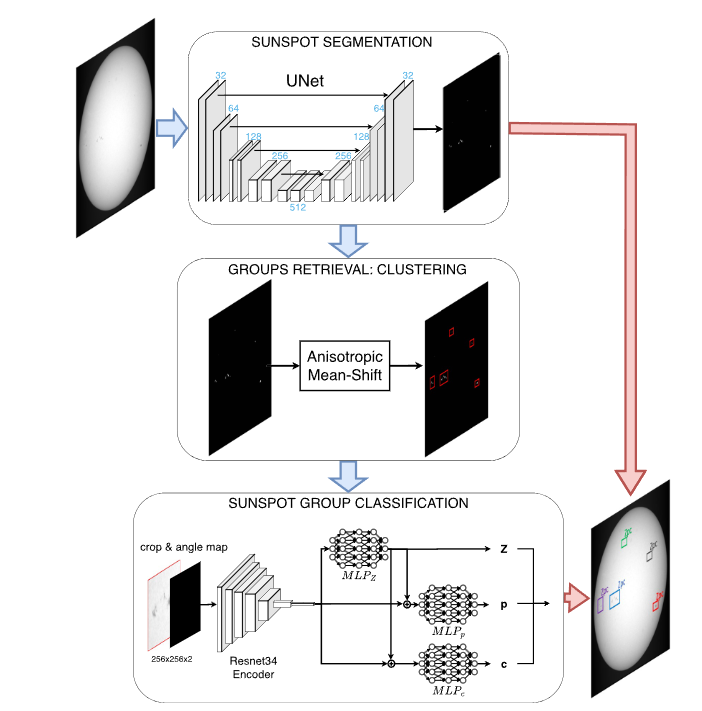
\includegraphics[width=0.5\textwidth]{figures/ml/yolo_train.png}
    \caption{Esquema del enfoque modular presentado por Sayez et al. \cite{sayez2023sunscc}, donde el flujo de procesamiento se modula en segmentación, agrupamiento y clasificación de manchas solares. \textbf{Fuente:} 
    Adaptado de Sayez et al..}
    \label{fig:sunscc_pipeline_stateoftheart}
\end{figure}

Este enfoque refleja mejor la lógica observacional de la taxonomía Zurich--McIntosh y, además, es el que mejores resultados comparativos reporta hasta la fecha entre los trabajos de referencia considerados en esta tesis Sayez et al. \citep{sayez2023sunscc,deng2025mcintosh}.

En consecuencia, el hilo conductor de este apartado consiste en examinar, primero, cómo se construye la unidad observacional relevante o grupo solar, y seguidamente, cómo dicha unidad se clasifica morfológicamente de forma automática.


\subsubsection{Agrupamiento de manchas solares}

La detección precisa de las manchas solares es fundamental para la construcción de índices de actividad solar (Número de Wolf; \citep{clette2007wolf}), y constituye además el punto de partida para cualquier procedimiento automático de agrupamiento y clasificación \citep{clette2007wolf,sayez2023sunscc}. Sin embargo, la delineación de manchas no es un problema completamente objetivo. Distintos observadores pueden discrepar en los bordes o en la separación de estructuras cercanas; además, las manchas presentan formas irregulares, contraste variable con la fotosfera y diferentes niveles de degradación cuando las imágenes provienen de observatorios terrestres.

En este contexto, la literatura reporta dos grandes familias de métodos de detección automática. Por un lado, los métodos basados en regiones utilizan umbralado, histogramas de intensidad con enfoques bayesianos o procedimientos de crecimiento de regiones para separar las manchas del fondo fotosférico a partir de propiedades radiométricas y de conectividad local \citep{pettauer1997sunspots,steinegger1998thresholds,turmon2002pattern,murakozy2022asymmetries}. Por otro lado, los métodos basados en bordes se concentran en las discontinuidades de la imagen y en la localización de contornos, a menudo complementados con operaciones de morfología matemática sobre imágenes de continuo \citep{zharkov2005automated,scherrer1995mdi,curto2008morphology,watson2009wilson}.

Una referencia importante en esta comparación es el trabajo de Carvalho et al. \citep{carvalho2020comparison}, donde muestran que los enfoques basados en morfología matemática tienden a comportarse mejor que los métodos puramente basados en intensidad. Además, requieren menos preprocesamiento para atenuar efectos atmosféricos y corregir el oscurecimiento hacia el limbo. No obstante, estos métodos siguen dependiendo en gran medida de elecciones heurísticas, como el tamaño de los operadores morfológicos o la fijación de umbrales, lo que limita su robustez frente a variaciones instrumentales y observacionales.

La literatura ha explorado diversas estrategias para resolver este problema. Nguyen et al. \citep{nguyen2004learning} evaluaron algoritmos jerárquicos y un esquema simple de \textit{k-means}, mostrando que este último resulta poco práctico cuando el número de grupos presentes en una observación no es conocido de antemano. Del mismo modo, los métodos jerárquicos dependen fuertemente del criterio de parada. En un trabajo posterior, los mismos autores compararon estas estrategias con DBSCAN y reportaron un comportamiento ligeramente mejor de los enfoques basados en densidad \citep{nguyen2006hybrid,ester1996dbscan}.

Dentro de este panorama, el algoritmo \textit{mean-shift} resulta especialmente atractivo porque permite localizar máximos locales de densidad en el espacio de observación e incorporar, de manera natural, conocimiento previo sobre la elongación anisotrópica de los clústeres. Esta propiedad lo vuelve particularmente adecuado para el problema solar, ya que los grupos de manchas muestran una organización longitudinal dominante. Por ello, la revisión más reciente considera que el agrupamiento debe diseñarse como una etapa independiente entre la detección de manchas y la clasificación del grupo, y no como una simple extensión geométrica de la segmentación \citep{comaniciu2002mean,sayez2023sunscc}.

En paralelo a estos métodos geométricos, los detectores de la familia YOLO han adquirido relevancia por formular la detección como un problema integrado de estimación de clases y cajas delimitadoras, con tiempos de inferencia compatibles con aplicaciones de baja latencia. Frente a modelos previos de la misma familia, YOLO26 enfatiza una arquitectura más simple y directamente desplegable: adopta una formulación nativa \textit{end-to-end}, reduce la dependencia de etapas externas de posprocesamiento y elimina la supresión no máxima (NMS) como requisito operativo. Esta diferencia es relevante porque, en variantes tradicionales, la salida del modelo suele requerir un procedimiento posterior para filtrar predicciones redundantes; al incorporar dicha resolución dentro del propio esquema de inferencia, se reduce la complejidad operacional, se simplifica la exportación y se facilita la ejecución en dispositivos de borde.

La propuesta también se distancia de versiones anteriores al retirar la formulación DFL, que aunque resulta útil para refinar la regresión de cajas, puede introducir complejidad adicional en la exportación y reducir compatibilidad con ciertos aceleradores o entornos de bajo consumo. A esto se suman innovaciones de entrenamiento, como el optimizador MuSGD y mejoras de pérdida orientadas a objetos pequeños, además de módulos específicos para segmentación, pose y detección orientada. En conjunto, estas decisiones apuntan a mantener precisión competitiva con menor costo de integración, y la documentación técnica reporta mejoras de velocidad de inferencia en CPU de hasta el 43\% respecto de configuraciones anteriores bajo sus condiciones de evaluación \citep{ultralyticsYOLO26}. En el contexto de esta tesis, esta orientación resulta pertinente porque el detector debe operar sobre imágenes solares completas, localizar estructuras de bajo tamaño relativo y conservar viabilidad computacional en un entorno de adquisición local.

La comparación con YOLOv8 y YOLO11 debe plantearse en función del escenario de despliegue. Ambas arquitecturas constituyen alternativas consolidadas para detección general, con disponibilidad de pesos preentrenados y desempeño robusto en bancos de prueba estándar; no obstante, su cadena de inferencia puede conservar dependencias de posprocesamiento o relaciones menos favorables entre precisión, latencia y costo de exportación cuando se prioriza ejecución en CPU o hardware embebido. Para una aplicación astronómica local, donde la inferencia debe repetirse sobre secuencias de imágenes solares y donde las manchas ocupan una fracción reducida del disco, YOLO26 ofrece una ventaja técnica al reducir la complejidad de despliegue y priorizar un equilibrio más explícito entre exactitud, velocidad y tamaño del modelo. Por ello, frente a YOLOv8 o YOLO11, su interés no se limita a una mejora de métrica aislada, sino a una adecuación más directa a sistemas de monitoreo solar ejecutados en nodos de borde.

\begin{figure}[H]
    \centering
    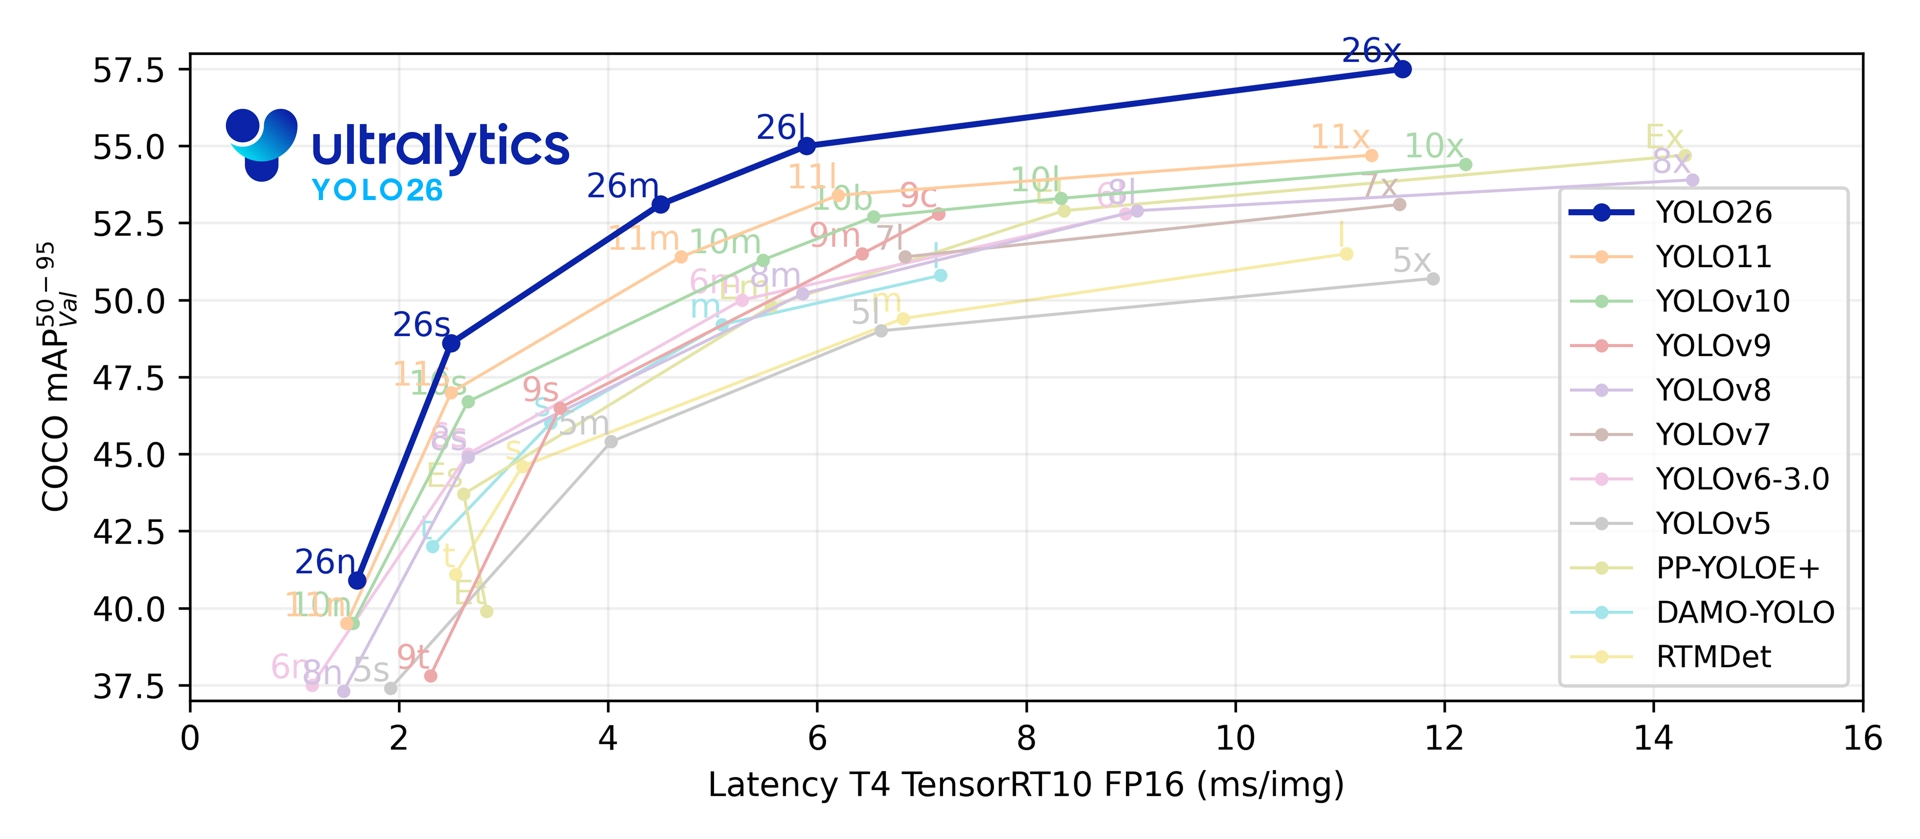
\includegraphics[width=0.92\textwidth]{figures/ml/yolo_bench.jpg}
    \caption{Comparación de desempeño de Ultralytics YOLO26 frente a modelos YOLO previos. La gráfica resume el compromiso entre precisión, velocidad y tamaño de las variantes, destacando la orientación de YOLO26 hacia inferencia eficiente y despliegue en escenarios con recursos restringidos. Adaptado de.}
    \label{fig:yolo26-benchmark}
\end{figure}

Esta discusión permite interpretar la elección de YOLO no solo como una decisión de precisión, sino como una decisión de arquitectura orientada al despliegue. Para un sistema de monitoreo solar, el detector debe localizar manchas pequeñas dentro de imágenes de disco completo, mantener tiempos de respuesta compatibles con adquisición continua y, al mismo tiempo, evitar una carga computacional excesiva en hardware local. En ese marco, la comparación de variantes resulta útil para evaluar el compromiso entre exactitud, latencia y tamaño del modelo.

La Figura~\ref{fig:yolo26-benchmark} sintetiza precisamente este posicionamiento: YOLO26 no se presenta únicamente como una iteración de mayor precisión, sino como una familia optimizada para equilibrar desempeño y complejidad de despliegue. La variante nano, YOLO26n, es la más adecuada cuando el objetivo no es maximizar la precisión en un servidor de entrenamiento, sino sostener inferencia rápida sobre hardware restringido. Para entrada de $640\times640$ píxeles, la documentación de referencia reporta aproximadamente $2.4$ millones de parámetros y $5.4$ GFLOPs en el modelo fusionado, con una precisión COCO mAP$_{50:95}$ de $40.9$ y tiempos de inferencia CPU--ONNX del orden de decenas de milisegundos bajo el entorno de evaluación reportado \citep{ultralyticsYOLO26}. Esta escala paramétrica es importante para el problema solar: las manchas ocupan áreas relativamente pequeñas dentro del disco completo, por lo que se requiere una arquitectura capaz de conservar sensibilidad espacial sin volver inviable la ejecución local.


\subsubsection{Clasificación morfológica de grupos solares}

La segunda etapa del problema corresponde a la clasificación morfológica de los grupos solares ya delimitados. A pesar de que las reglas de clasificación están formalmente establecidas, esta tarea continúa realizándose manualmente en numerosos observatorios y sigue estando expuesta a subjetividad, sesgos entre observadores y discrepancias en la interpretación de configuraciones morfológicas cercanas.

Las primeras propuestas automáticas combinaron umbralado, reglas manuales y clasificadores poco profundos sobre imágenes de continuo y magnetogramas. Aunque estos trabajos constituyen antecedentes importantes, muchos de ellos se validaron sobre conjuntos de datos reducidos o simplificados, lo que limita la generalización de sus resultados. Más recientemente, la clasificación automática ha pasado a apoyarse en CNN, aprendizaje por transferencia y esquemas multitarea capaces de predecir las componentes de la taxonomía Zurich--McIntosh de manera más estructurada.

En este contexto, Palladino et al. \citep{palladino2022sunspot} abordan la tarea mediante detección y clasificación apoyadas en imágenes de continuo, magnetogramas y tablas SRS, observando que la confusión entre clases cercanas del componente $Z$ en particular entre D, E y F sigue siendo una de las principales dificultades del problema. Por su parte, Sayez et al. \citep{sayez2023sunscc} formulan la clasificación como un problema jerárquico, donde las componentes $Z$, $P$ y $C$ se predicen de manera dependiente y se complementan con agregación de clases y ensambles para estimar confiabilidad. Esta estrategia resulta especialmente relevante para esta tesis porque preserva la estructura semántica de la clasificación en el propio diseño del modelo.

La literatura reciente muestra además dos tendencias complementarias. Una busca mantener la taxonomía completa para conservar riqueza observacional y trazabilidad; la otra simplifica el espacio de clases o predice por componentes para estabilizar el aprendizaje en escenarios con fuerte desbalance. En esa línea, Zhou et al. \citep{zhou2023mcintosh} subrayan la necesidad de ampliar y depurar las bases de datos McIntosh, mientras que trabajos más recientes como Deng et al. \citep{deng2025mcintosh} continúan explorando arquitecturas profundas para clasificación morfológica fina.

Dentro de este escenario, ConvNeXtV2 representa una alternativa relevante frente a CNN clásicas y arquitecturas basadas exclusivamente en transformadores. Su interés proviene de modernizar una red convolucional pura con decisiones inspiradas por los avances recientes en visión: bloques residuales profundos, convoluciones de gran campo efectivo, normalización por capas, activaciones suaves y una organización por etapas que facilita transferencia de aprendizaje. La segunda versión añade una capa de \textit{Global Response Normalization} (GRN) y se co-diseña con un esquema de preentrenamiento auto-supervisado mediante \textit{Fully Convolutional Masked Autoencoder} (FCMAE), lo que mejora la competencia entre canales y la calidad de las representaciones aprendidas \citep{woo2023convnextv2}.

\begin{figure}[H]
  \centering
  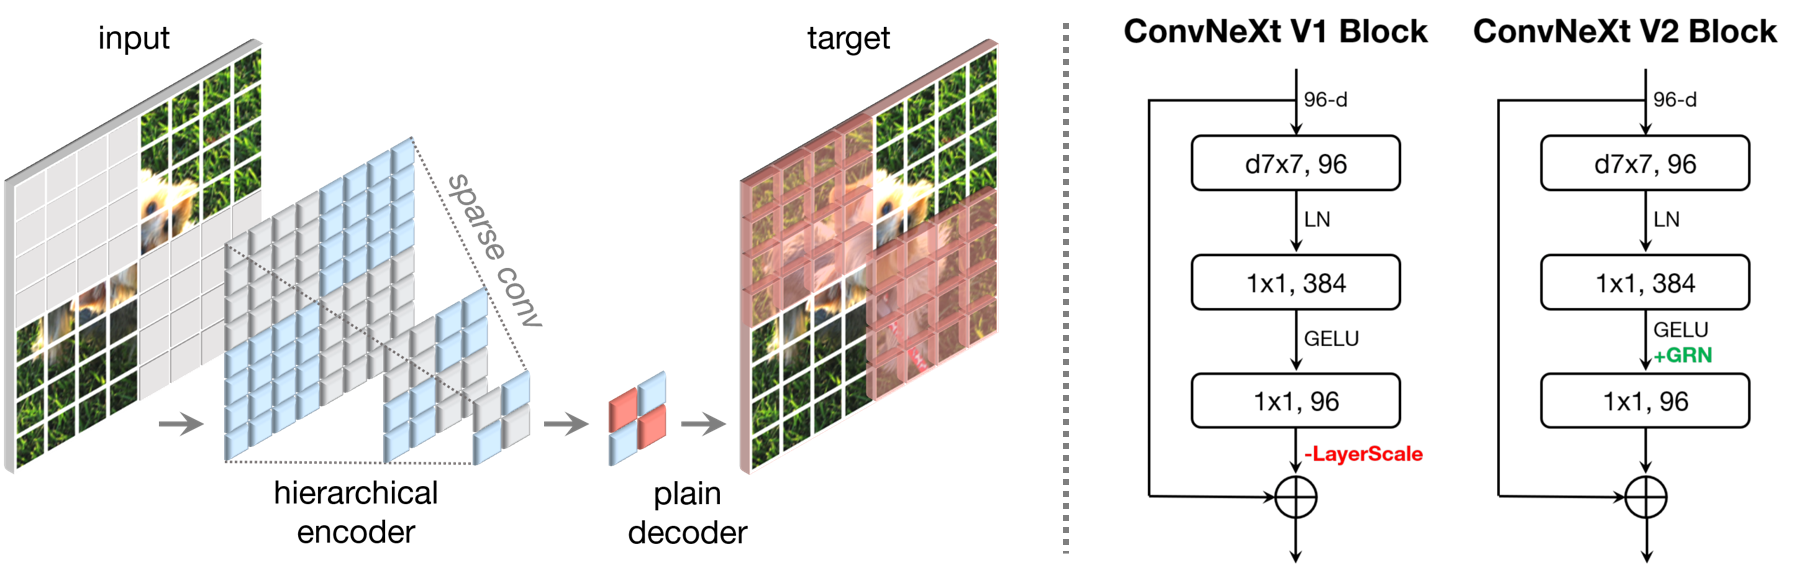
\includegraphics[width=0.82\textwidth]{figures/ml/fcmae.png}
  \caption{Esquema de preentrenamiento FCMAE empleado en ConvNeXtV2. La estrategia enmascara regiones de entrada y fuerza al codificador convolucional a reconstruir información visual faltante, favoreciendo representaciones robustas antes del ajuste supervisado. \textbf{Fuente:} Adaptado de Woo et al..}
  \label{fig:convnextv2-fcmae}
\end{figure}

El esquema de la Figura~\ref{fig:convnextv2-fcmae} es especialmente pertinente para clasificación morfológica porque desplaza parte del aprendizaje desde etiquetas discretas hacia la estructura visual de las imágenes. En un problema como Zurich--McIntosh, donde las clases pueden diferir por continuidad penumbral, compactación o distribución interna de manchas, este tipo de preentrenamiento resulta útil para inicializar extractores de características sensibles a textura, contorno y organización espacial del grupo solar.

\begin{figure}[H]
  \centering
  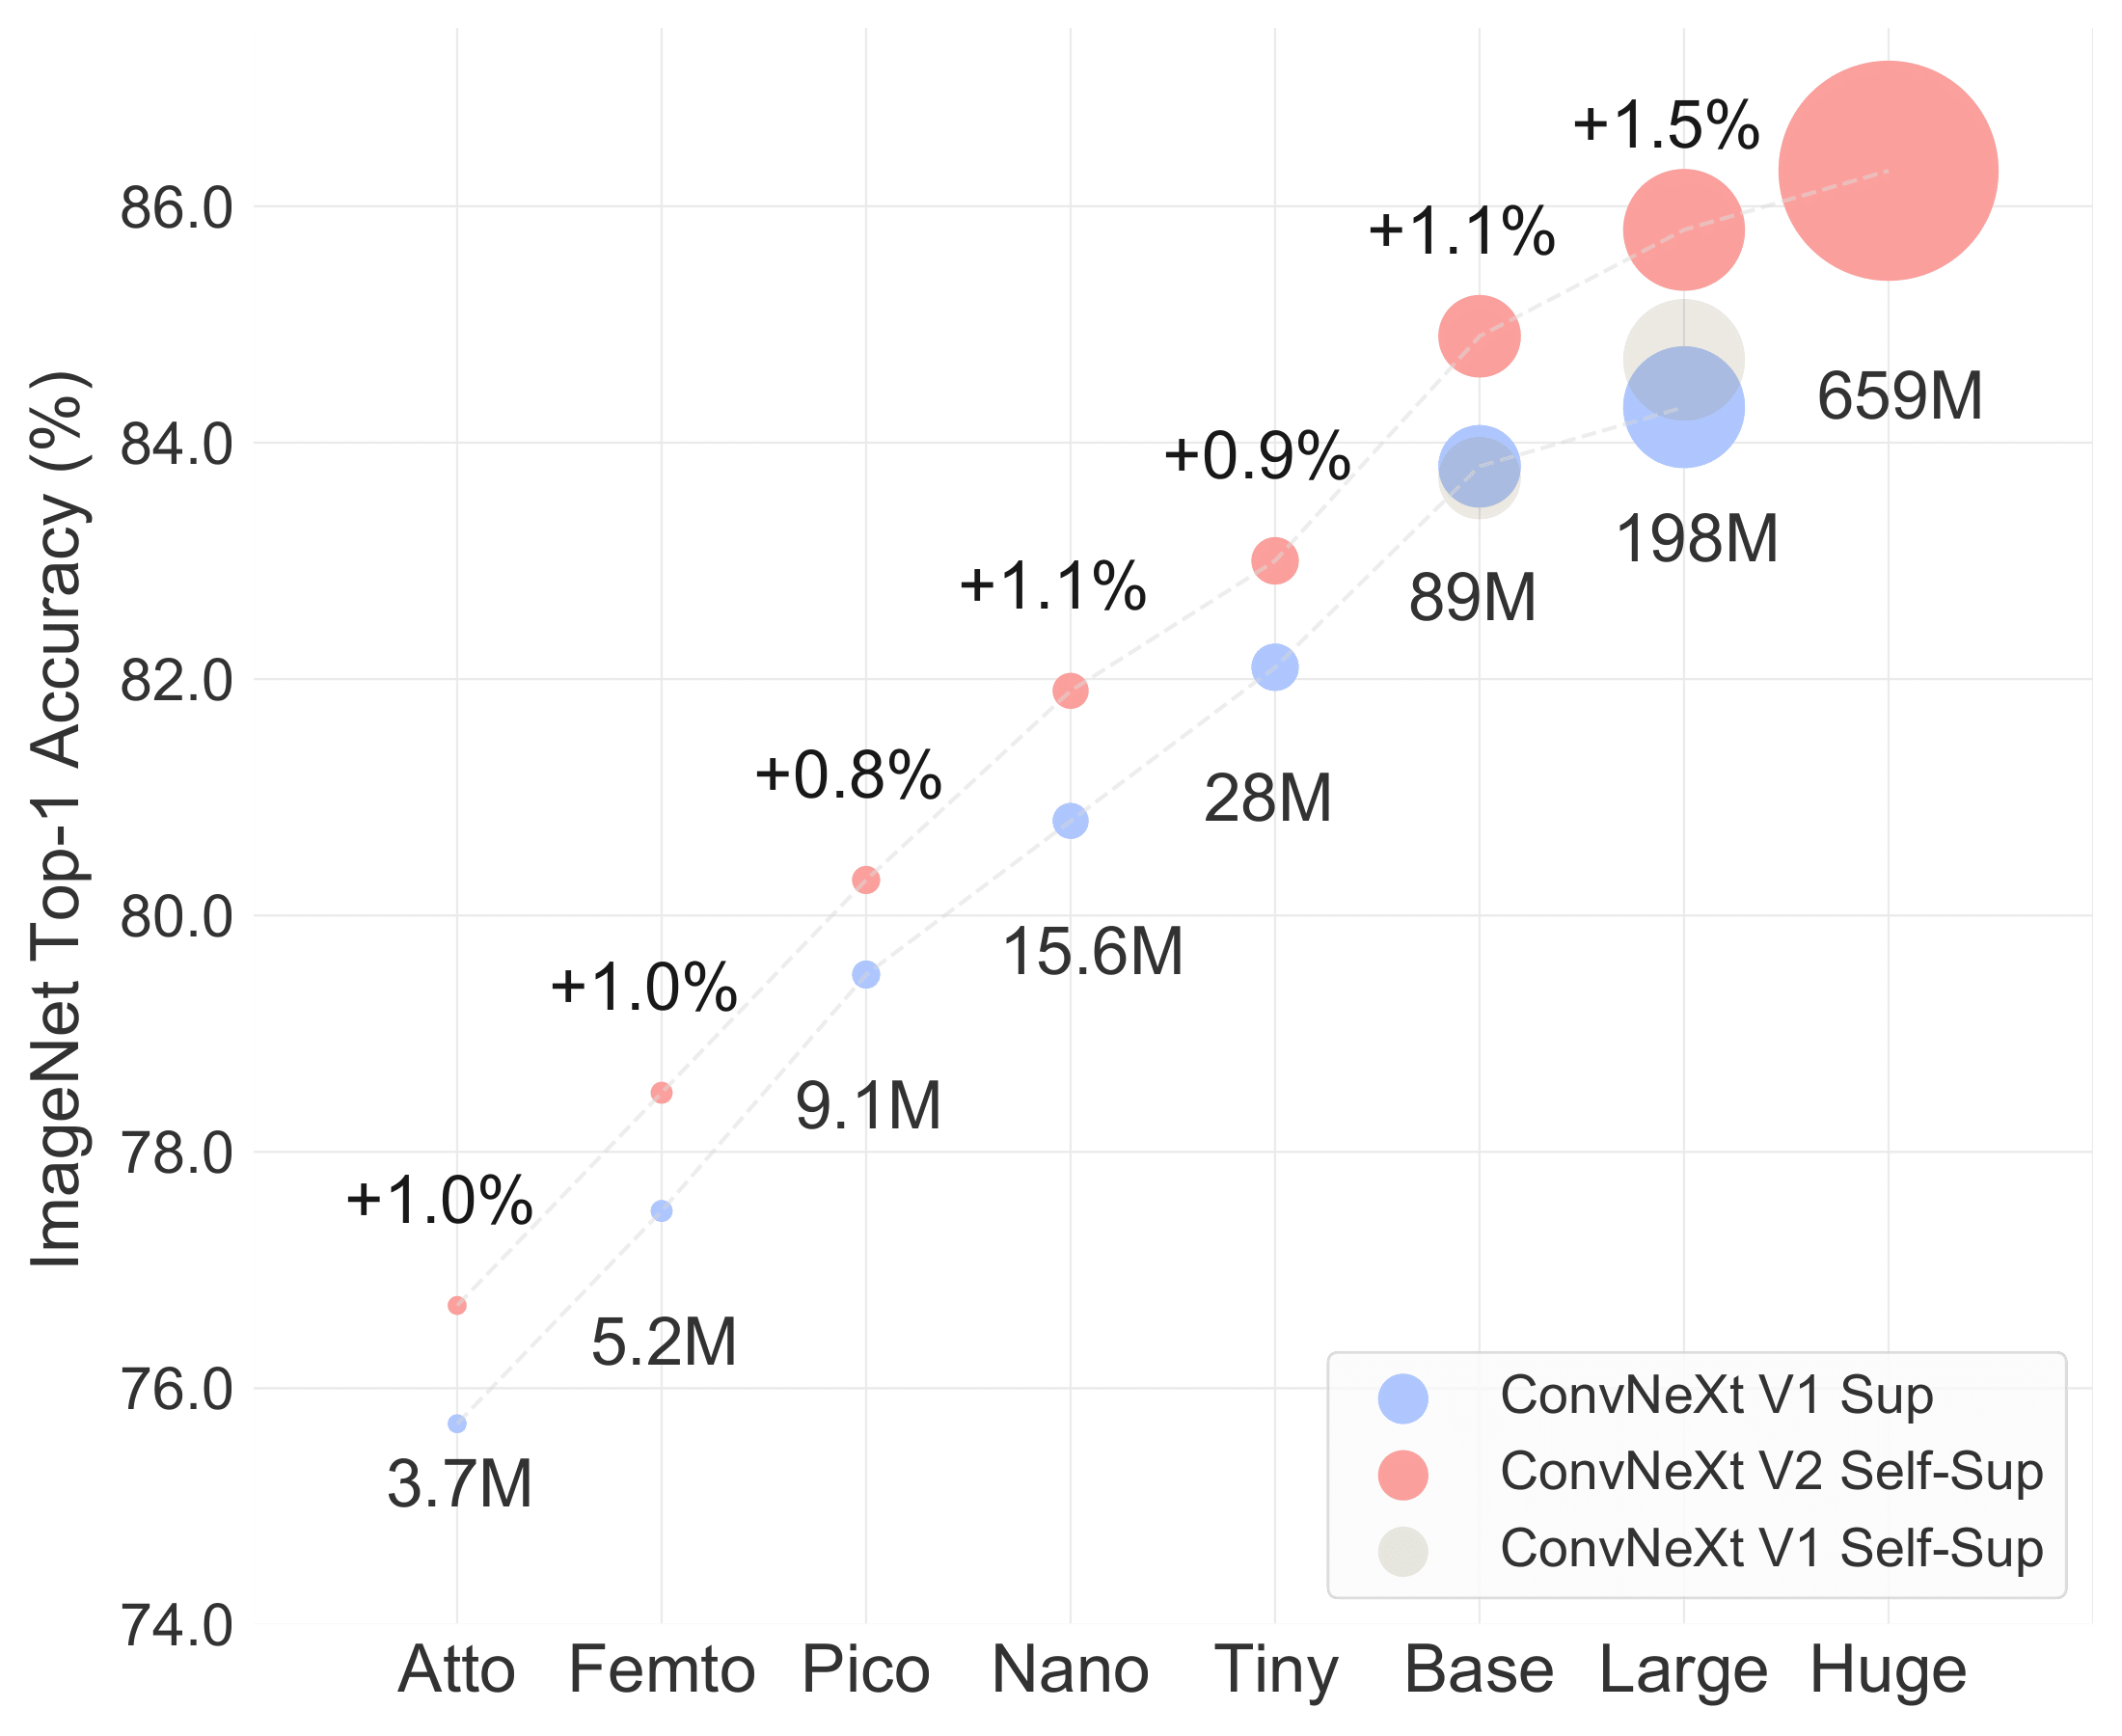
\includegraphics[width=0.82\textwidth]{figures/ml/scaling.png}
  \caption{Escalamiento de modelos ConvNeXtV2 y relación entre tamaño de red, capacidad representacional y desempeño. La figura muestra cómo la familia organiza variantes de distinta complejidad, desde configuraciones compactas hasta modelos de mayor escala. \textbf{Fuente:} Adaptado de Woo et al..}
  \label{fig:convnextv2-scaling}
\end{figure}

La Figura~\ref{fig:convnextv2-scaling} permite contextualizar la selección de una variante compacta dentro de la familia ConvNeXtV2 \citep{woo2023convnextv2}. En este trabajo se adopta \texttt{ConvNeXtV2\_atto}, la configuración más ligera de la familia, porque ofrece un compromiso adecuado entre capacidad representacional, estabilidad de exportación y costo de despliegue. Esta elección no busca maximizar el tamaño del extractor, sino preservar la integridad de la red durante la transformación desde PyTorch hacia ONNX y facilitar su distribución en entornos con recursos limitados. Aun con esta escala compacta, el backbone conserva profundidad suficiente para capturar textura, penumbra, fragmentación interna y extensión global del grupo solar \citep{woo2023convnextv2}. Esta característica es especialmente útil para la clasificación Zurich--McIntosh, donde las diferencias entre clases no dependen solo de la presencia de manchas, sino de patrones morfológicos sutiles como continuidad penumbral, compactación, separación longitudinal y distribución de manchas intermedias. Frente a CNN más antiguas, ConvNeXtV2 conserva el sesgo inductivo local de la convolución, favorable para texturas fotosféricas, pero incorpora mejoras de escalamiento y entrenamiento que lo acercan al rendimiento de arquitecturas modernas. Frente a transformadores visuales, mantiene una implementación más directa para recortes de tamaño moderado y se adapta de forma natural a salidas MLP multisalida para aprendizaje jerárquico.

\subsection{Modelos predictivos de la actividad solar}

El análisis de la actividad fotosférica ha evolucionado desde la simple observación morfológica hacia la construcción de marcos predictivos que buscan anticipar la evolución temporal del ciclo solar. Este problema es de naturaleza compleja, ya que el número, el área y la distribución latitudinal de las manchas solares responden a una modulación asimétrica y estocástica que dificulta los pronósticos de largo plazo \citep{pesnell2012predictions}. En la literatura actual, las estrategias para abordar esta variabilidad se dividen principalmente entre métodos de precursores físicos, modelos estadísticos de series temporales y, más recientemente, enfoques basados en aprendizaje automático, identificación dinámica y descomposición de señales \citep{clette2014revisiting}.

Dentro de los métodos operativos más consolidados, el uso de precursores basados en los campos polares y los índices geomagnéticos ha demostrado ser eficaz para estimar la amplitud del máximo de un ciclo con varios años de antelación \citep{schatten2005precursor,svalgaard2005polar}. Sin embargo, estos enfoques a menudo carecen de la resolución temporal necesaria para describir la evolución mensual de la actividad. Para subsanar esta limitación, se han desarrollado técnicas de filtrado adaptativo que permiten una actualización recursiva de las predicciones a medida que se disponen de nuevos registros mensuales.

El índice más utilizado para representar esa evolución temporal es el número de manchas solares o SSN, históricamente conocido como número de Wolf. En su formulación clásica, este índice combina el número de grupos solares observados y el número total de manchas individuales mediante una expresión del tipo $R=k(10g+s)$, donde $g$ representa los grupos, $s$ las manchas individuales y $k$ un factor de escala asociado al observador o instrumento. Su valor no debe interpretarse como un conteo físico directo, sino como un índice normalizado de actividad fotosférica que permite comparar observaciones realizadas bajo condiciones instrumentales y observacionales distintas \citep{clette2007wolf,clette2014revisiting}.

En este contexto, Podladchikova y Van der Linden \citep{podladchikova2012kalman} proponen una técnica de mejora basada en el filtro de Kalman adaptativo aplicada a predicciones del número de manchas solares suavizado. En una notación consistente con el modelo usado en la Sección~\ref{sec:forecast}, el pronóstico escalar puede formularse con un estado oculto $s_k\in\mathbb{R}$ asociado al SSN suavizado y una observación mensual $z_k\in\mathbb{R}$. La dinámica a priori se escribe como
\begin{equation}
\widehat{s}_{k}^{-}=\Phi_k\widehat{s}_{k-1},
\end{equation}
donde $\widehat{s}_{k}^{-}$ es la estimación previa al incorporar la observación del mes $k$ y $\Phi_k$ representa el cambio relativo esperado de la curva guía del ciclo. La incertidumbre asociada se propaga mediante
\begin{equation}
P_k^{-}=\Phi_k^{2}P_{k-1}+Q_k,
\end{equation}
donde $P_k^{-}$ es la varianza a priori y $Q_k$ representa el ruido de proceso.

Para construir la transición $\Phi_k$, el modelo retoma el perfil analítico de ciclo introducido por Hathaway, Wilson y Reichmann \citep{hathaway2010solarcycle}. Si $v$ denota el tiempo transcurrido desde el inicio efectivo del ciclo, la forma base puede escribirse como
\begin{equation}
f(v;a,b)=\frac{a v^{3}}{\exp\!\left(v^{2}/b^{2}\right)-0.71},
\end{equation}
donde $a$ controla la amplitud y $b$ regula la anchura temporal del ciclo. En consecuencia, la transición entre instantes consecutivos se define como
\begin{equation}
\Phi_k=\frac{f(v_k;a,b)}{f(v_{k-1};a,b)}.
\end{equation}
La actualización con la observación disponible se realiza mediante la ganancia de Kalman
\begin{equation}
K_k=P_k^{-}\left(P_k^{-}+R_k\right)^{-1},
\end{equation}
y la corrección del estado queda dada por
\begin{equation}
\widehat{s}_{k}=\widehat{s}_{k}^{-}+K_k\left(z_k-\widehat{s}_{k}^{-}\right),
\end{equation}
donde $R_k$ es la varianza del ruido de medición. Así, la salida escalar del bloque predictivo puede denotarse como $\mathrm{SSN}_{\mathrm{PVLK}}(t_k)=\widehat{s}_{k}$, manteniendo la misma convención empleada en la formulación metodológica.

Paralelamente al desarrollo de estos modelos estadísticos unidimensionales, el auge de la heliofísica computacional ha impulsado el uso de arquitecturas de redes neuronales y otros modelos de aprendizaje estadístico \citep{camporeale2019ml}. Estos trabajos sugieren que la predictibilidad del Sol puede mejorar sustancialmente si se consideran regularidades no lineales que los modelos empíricos tradicionales suelen omitir. No obstante, un desafío persistente en estos métodos es la integración de la información latitudinal de manera coherente con la física de la dinamo.

En este escenario, surge el interés por las técnicas de descomposición modal aplicadas a datos vectorizados. La Descomposición en Modos Dinámicos (DMD) resulta especialmente adecuada para reproducir fenómenos dinámicos a partir de múltiples observaciones, porque estima un operador que relaciona instantáneas consecutivas del sistema y permite reconstruir su evolución dominante. Esta propiedad explica su uso extendido en modelos físicos de mecánica de fluidos y sistemas complejos \citep{schmid2010dmd,kutz2016dmd}, así como su incorporación reciente en métodos de identificación dinámica para algoritmos iterativos y problemas numéricos de gran escala \citep{benitez2026adaptive}.

Desde esta perspectiva, la presente tesis adopta el DMD como una línea propia de modelado para explorar la evolución latitudinal de la actividad solar. La idea central no se desarrolla aquí como parte del estado del arte, sino que se retoma metodológicamente en la Sección~\ref{sec:forecast}: tratar el diagrama de Spörer como una secuencia de observaciones espacio-temporales y derivar, a partir de su reconstrucción dinámica, una tendencia global comparable con los pronósticos escalares tradicionales. De este modo, el DMD se introduce en esta revisión principalmente como antecedente conceptual y como motivación para la propuesta predictiva desarrollada posteriormente. 
\chapter[Consideraciones de diseño]{Consideraciones de diseño\label{cap:consideraciones}}


El proyecto se organiza como un ecosistema modular desacoplado para la instrumentación, recopilación, procesamiento y análisis de manchas solares. Esta organización permite separar responsabilidades entre la adquisición local, la publicación de datos, el procesamiento mediante modelos de Deep Learning y el análisis predictivo de la actividad solar.

\begin{figure}[H]
    \centering
    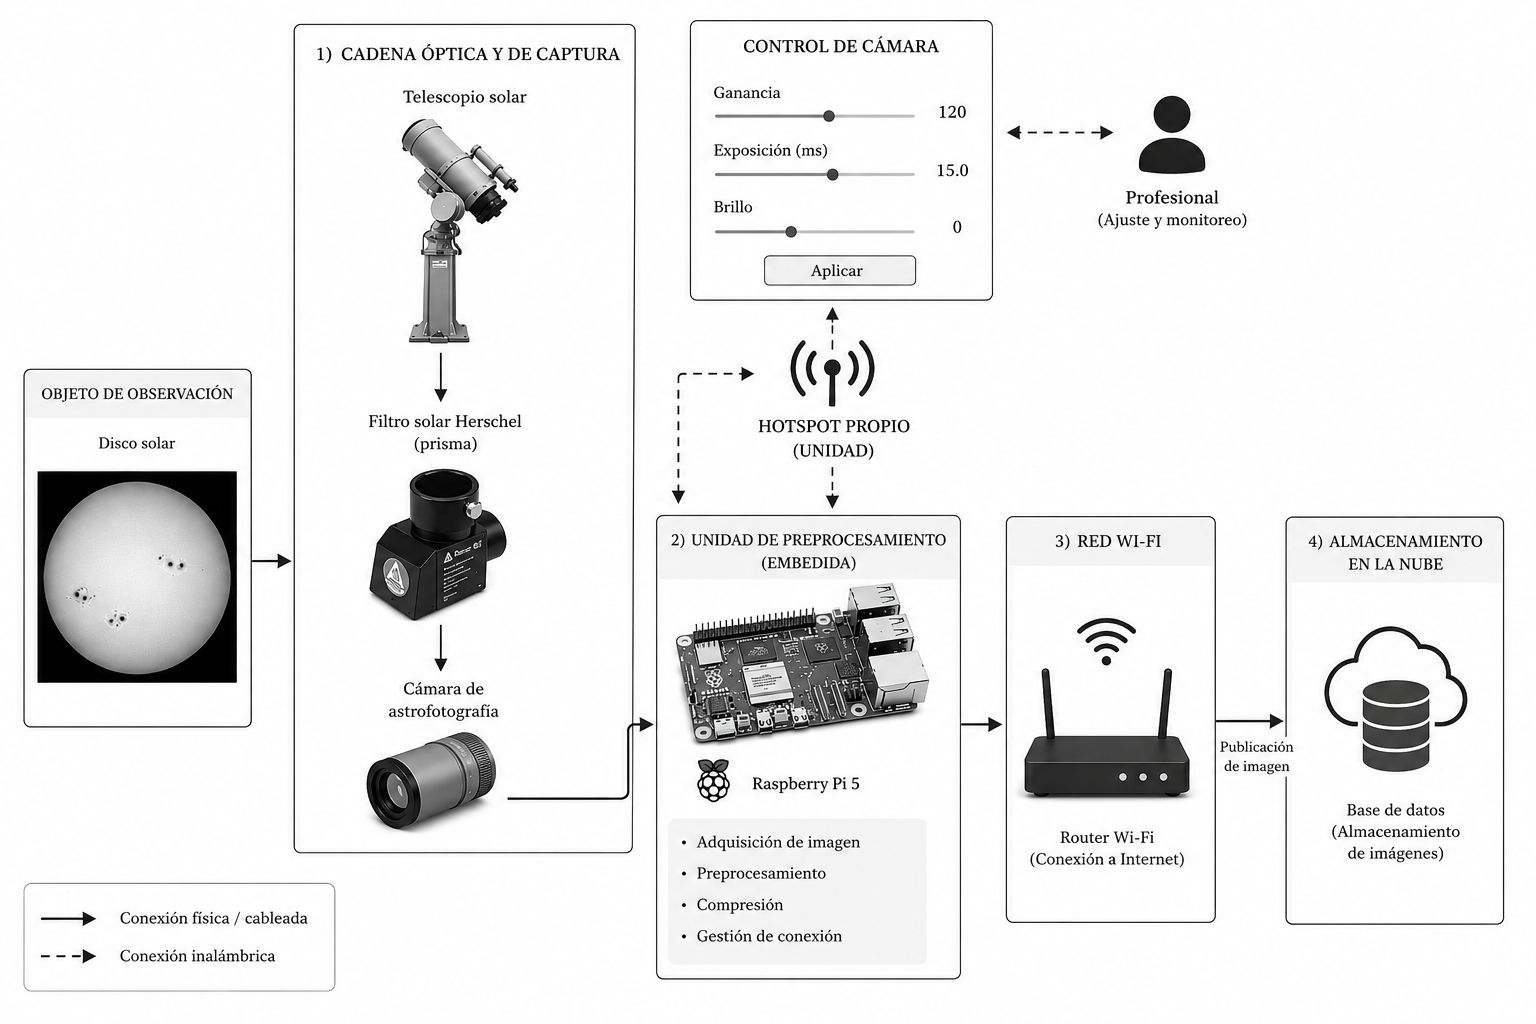
\includegraphics[width=\textwidth]{figures/hw/module.png}
    \caption{Flujo operativo de la etapa de preprocesamiento embebida. Se destaca la captura y calibración de imágenes de disco solar completo, la operación mediante panel web local y la publicación posterior hacia una base de datos en la nube. \textbf{Fuente:} Elaboración propia.}
    \label{fig:ecosistema-modular-general}
\end{figure}

La primera etapa corresponde a la unidad de preprocesamiento embebida. Esta unidad opera junto al sistema óptico de observación y cumple una función dual de conectividad: por un lado, despliega una zona WiFi propia para configuración directa en campo; por otro, puede conectarse como cliente a una red WiFi disponible para la publicación de datos. Desde esta unidad se gestionan la calibración, la captura de imágenes de disco solar completo y las tareas iniciales de preprocesamiento. La operación se controla mediante un panel web en la red local de la propia unidad, lo que permite ajustar parámetros de captura, supervisar el estado del dispositivo y coordinar el envío de observaciones sin depender de una estación externa permanente.

Una vez obtenidas y preprocesadas, las imágenes se envían desde el mismo dispositivo hacia una base de datos en la nube.

\begin{figure}[H]
    \centering
    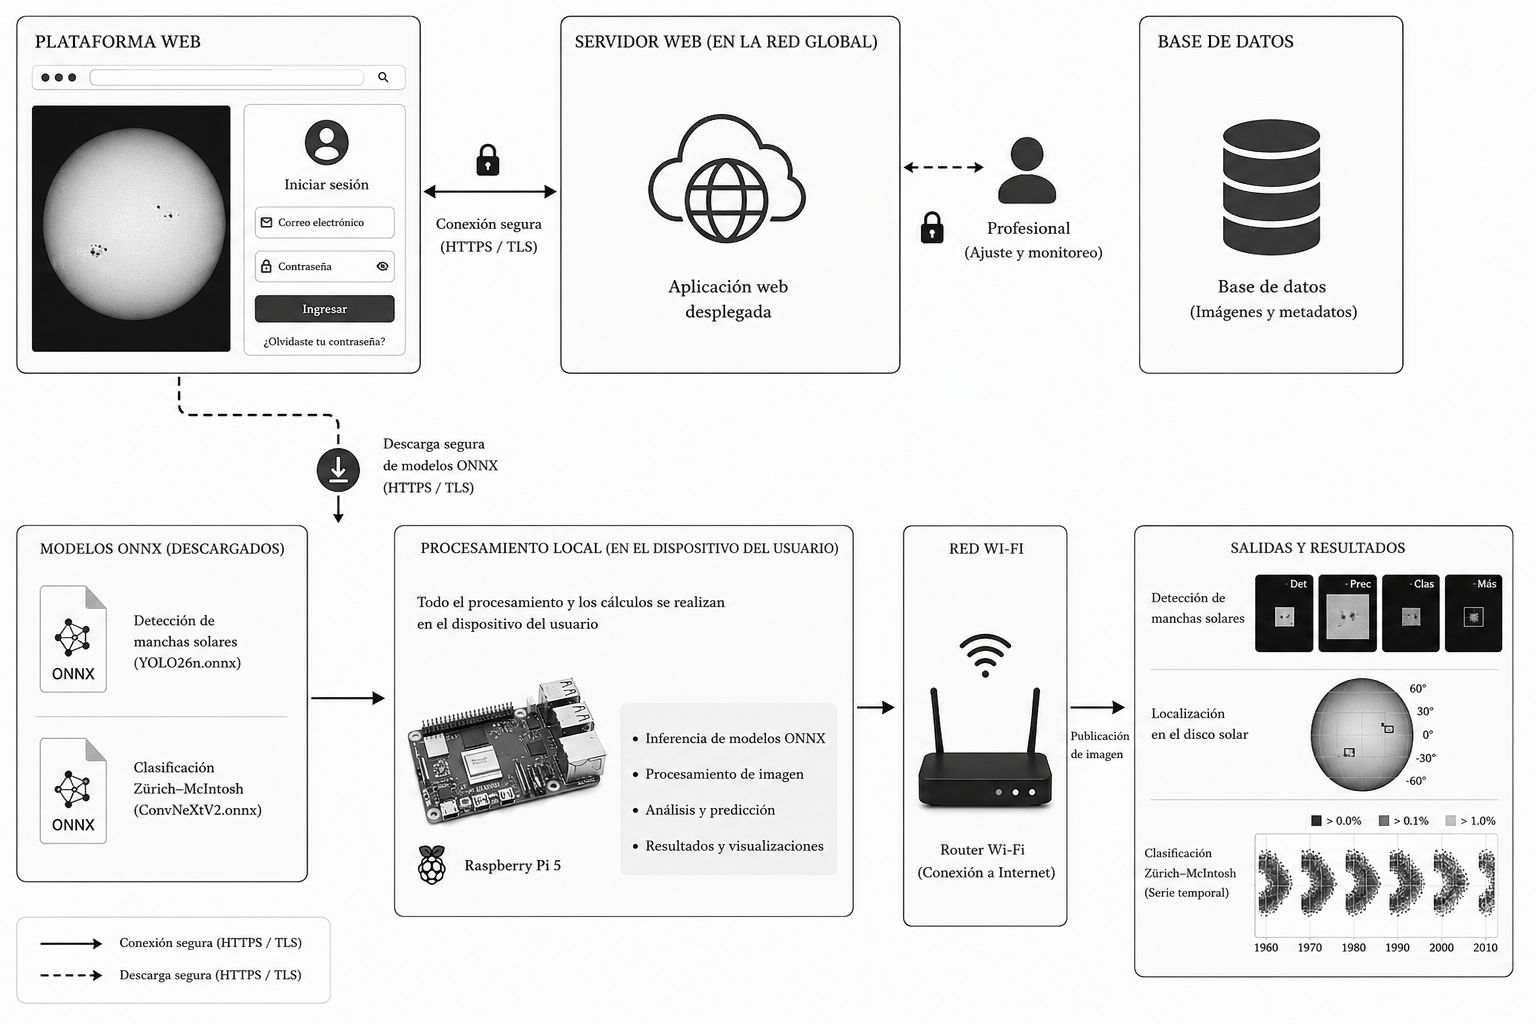
\includegraphics[width=\textwidth]{figures/hw/camera_mount.png}
    \caption{Flujo operativo de la etapa de procesamiento, agrupamiento y clasificación con ONNX y predicción de actividad solar. \textbf{Fuente:} Elaboración propia.}
    \label{fig:unidad-preprocesamiento-embebida}
\end{figure}

Esta base de datos actúa como repositorio intermedio para almacenar imágenes, metadatos y registros observacionales, desacoplando la etapa de adquisición de las etapas posteriores de consulta y análisis.

A partir de estos datos publicados, una segunda plataforma web de acceso abierto recopila y presenta la información disponible. En dicha plataforma se integran los modelos de Deep Learning para el procesamiento de imágenes y la clasificación Zurich--McIntosh, un apartado de tendencias que incorpora los modelos predictivos estudiados, y un apartado de registros destinado a visualizar tanto los datos recopilados para este trabajo como los obtenidos en el Observatorio Astronómico ``Prof. Alexis Troche Boggino''.

\begin{figure}[H]
    \centering
    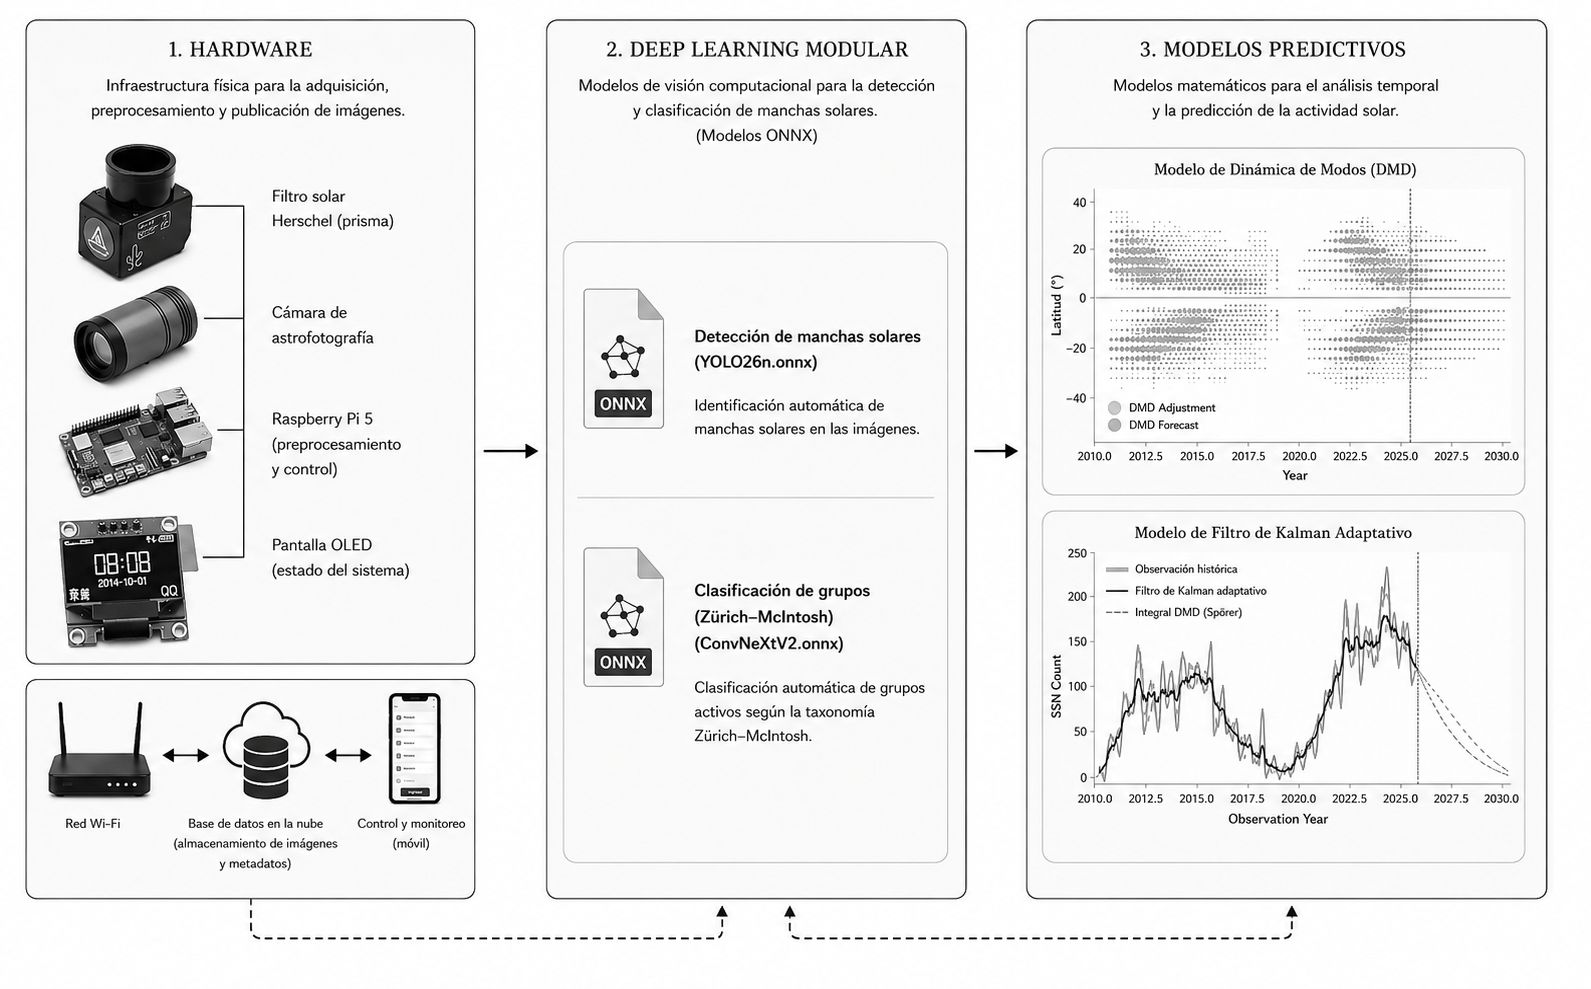
\includegraphics[width=\textwidth]{figures/hw/site_setup.png}
    \caption{Arquitectura integral del ecosistema de trabajo. La figura resume la relación entre la instrumentación solar, la unidad embebida de captura y preprocesamiento, la base de datos en la nube y la plataforma web abierta que integra clasificación Zurich--McIntosh, modelos de tendencias y registros observacionales. \textbf{Fuente:} Elaboración propia.}
    \label{fig:arquitectura-integral-ecosistema}
\end{figure}

La Figura~\ref{fig:arquitectura-integral-ecosistema} resume la relación entre estos elementos. El flujo general parte de la instrumentación solar, continúa con la unidad embebida de captura y preprocesamiento, publica las observaciones en una base de datos en la nube y culmina en una plataforma web abierta donde se concentran los módulos de análisis, visualización y consulta histórica.

En este contexto, las consideraciones de diseño del proyecto se presentan en tres secciones diferenciadas: \textit{hardware} e instrumentación, encargados de la adquisición de imágenes solares; Deep Learning, orientado al procesamiento visual y a la clasificación morfológica; y modelos predictivos, dedicados al análisis de tendencias de la actividad solar. La separación entre módulos permite que cada etapa pueda diseñarse, validarse y actualizarse de manera independiente, manteniendo al mismo tiempo una cadena completa desde la captura del disco solar hasta la interpretación científica de los datos.


\section{Hardware}

Como se indicó en la Sección~\ref{sec:physics}, el componente instrumental del proyecto se contextualiza en el Observatorio Astronómico ``Prof. Alexis Troche Boggino'' y en su infraestructura de supervisión y registro, mostrada en la Figura~\ref{fig:observatorio-alexis-troche}. A partir de ese entorno local, esta sección se concentra en la cadena de hardware específica del prototipo.

Para el prototipo se considera una cadena de instrumentación para luz blanca compuesta por un telescopio refractor Vixen con diámetro $D=60\,\mathrm{mm}$ y distancia focal $F=420\,\mathrm{mm}$, una cámara monocromática y un filtro de atenuación óptica adecuado para observación solar. Este conjunto establece las condiciones de exposición, contraste, campo de visión y estabilidad mecánica sobre las que luego operan las etapas de preprocesamiento y análisis. El uso de un refractor pequeño favorece la portabilidad, reduce exigencias mecánicas, facilita la alineación en pruebas de campo y permite implementar medidas de seguridad óptica con menor complejidad que en instrumentos de mayor apertura. Posteriormente, se selecciona la plataforma base para el desarrollo del módulo de adquisición de imagen y preprocesamiento embebido.

\subsection{Cámara de astrofotografía solar}

La selección de la cámara se abordó como una exploración del mercado de sensores monocromáticos empleados en imagen solar de alta cadencia. Dado que la cámara seleccionada debe integrarse en un tren óptico compacto y ofrecer una base útil para captura solar rápida, la comparación se centra en prestaciones directamente vinculadas con ese objetivo: área sensora, resolución espacial, tamaño de píxel, tipo de obturador, conversión ADC, interfaz y precio referencial. La Tabla~\ref{tab:comparacion_camaras_proyecto} resume estas variables para un conjunto de alternativas monocromáticas disponibles comercialmente \citep{zwoASI174Manual2025,zwoGuideCameras2025,qhyQHY5III6782026,qhyMiniCAM8M2026,playerOneApolloMMax2026}.

\begin{table}[H]
\centering
\caption{Exploración de cámaras monocromáticas disponibles comercialmente para captura solar de alta cadencia y guiado. Los precios son referenciales y pueden variar según distribuidor, región y fecha de consulta. \textbf{Fuente:} Elaboración propia.}
\label{tab:comparacion_camaras_proyecto}
\uniformtablestyle
\begin{tabularx}{\textwidth}{>{\raggedright\arraybackslash}p{2.9cm} >{\raggedright\arraybackslash}p{2.8cm} >{\raggedright\arraybackslash}p{2.15cm} >{\centering\arraybackslash}p{1.3cm} X}
\toprule
\textbf{Fabricante / modelo} & \textbf{Sensor / muestreo} & \textbf{Conversión / interfaz} & \textbf{Precio ref.} & \textbf{Observaciones} \\
\midrule
QHYCCD QHY5III678M & IMX678, 7.71\,mm $\times$ 4.36\,mm; 3856$\times$2180; 2.0\,$\mu$m & 12-bit ADC; USB3.0 Tipo-C; buffer 512 MB & US\$384 & Destaca por su resolución de 8.4 MP y por un muestreo fino basado en píxeles de 2.0\,$\mu$m. \\
ZWO ASI174MM Mini & IMX174LLJ/LQJ, 11.3\,mm $\times$ 7.1\,mm; 1936$\times$1216; 5.86\,$\mu$m & 12-bit ADC; QE pico 77\%; USB2.0 Tipo-C & US\$432 & Destaca por combinar sensor de 1/1.2\,$''$, obturador global y píxeles de 5.86\,$\mu$m en formato mini. \\
QHYCCD miniCAM8M & IMX585, 11.2\,mm $\times$ 6.3\,mm; 3856$\times$2180; 2.9\,$\mu$m & Dual 12-bit ADC; USB3.0; TEC; carrusel 8 pos. & US\$599 & Destaca por integrar refrigeración TEC y carrusel de filtros en un cuerpo orientado a captura más versátil. \\
Player One Apollo-M MAX & IMX432, 14.5\,mm $\times$ 9.9\,mm; 1608$\times$1104; 9.0\,$\mu$m & 12-bit ADC; USB3.0; obturador global & US\$618 & Destaca por su área sensora amplia y por píxeles de 9.0\,$\mu$m orientados a alta señal por píxel. \\
\bottomrule
\end{tabularx}
\end{table}

A partir de esta comparación se adopta la ZWO ASI174MM Mini como dispositivo principal de captura. Su rasgo diferencial dentro del conjunto evaluado es la combinación entre sensor de 1/1.2\,$''$, obturador global, píxel de 5.86\,$\mu$m y cuerpo mini, una combinación poco frecuente cuando se busca compatibilidad con trenes ópticos compactos sin comprometer el campo útil ni la robustez temporal en secuencias rápidas \citep{zwoASI174Manual2025,zwoGuideCameras2025,qhyQHY5III6782026,qhyMiniCAM8M2026,playerOneApolloMMax2026}.

\begin{figure}[H]
    \centering
    \begin{subfigure}[t]{0.47\textwidth}
        \centering
        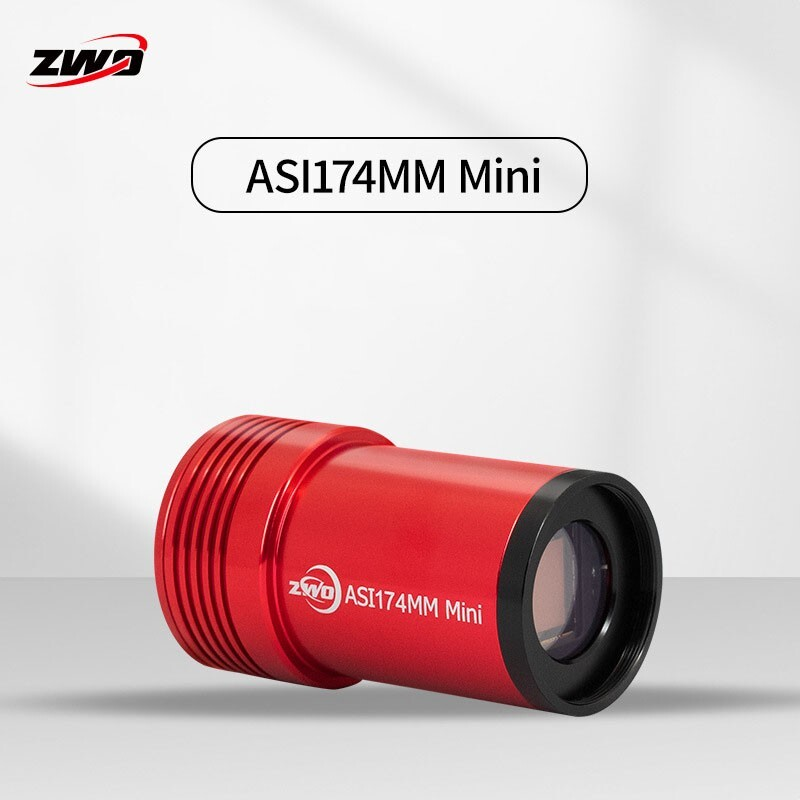
\includegraphics[width=\textwidth]{figures/hw/pi5.jpg}
        \caption{Vista general de la cámara ZWO ASI174MM Mini empleada como dispositivo de captura en el prototipo.}
    \end{subfigure}
    \hfill
    \begin{subfigure}[t]{0.47\textwidth}
        \centering
        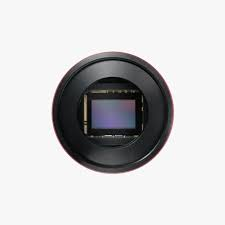
\includegraphics[width=\textwidth]{figures/hw/asi174.jpg}
        \caption{Vista frontal del sensor, donde se aprecia el área sensible del detector CMOS monocromático.}
    \end{subfigure}
    \caption{Cámara ZWO ASI174MM Mini considerada para el prototipo de observación solar. Se muestran (a) la vista general del cuerpo de cámara y (b) la vista frontal del sensor. \textbf{Fuente:} página oficial de ZWO (ZWO Astronomy Cameras).}
    \label{fig:zwo_project_camera}
\end{figure}

La documentación técnica de ZWO reporta para este modelo un área efectiva de 11.3\,mm $\times$ 7.1\,mm, conversión ADC de 12 bits y un QE pico de 77\%. Dentro de la serie mini, además, el fabricante la presenta como la opción de mayor campo y como una cámara pensada para integrarse mecánicamente de forma semejante a un ocular, rasgo relevante para el montaje previsto en este trabajo \citep{zwoASI174Manual2025,zwoGuideCameras2025}.

Desde una perspectiva observacional, el uso de \textit{global shutter} que integra esta cámara contribuye a reducir distorsiones temporales entre líneas y favorece la captura de secuencias rápidas en presencia de \textit{seeing} variable. Asimismo, el carácter monocromático del sensor evita la interpolación cromática asociada a matrices Bayer y conserva mejor la nitidez espacial efectiva. En conjunto, estas propiedades hacen que la cámara resulte particularmente adecuada para registrar estructuras fotosféricas con un balance favorable entre señal por píxel, estabilidad temporal y simplicidad de integración \citep{sonyPregiusGlobalShutter,zwoASI174Manual2025}.

Desde el punto de vista operativo, la combinación entre exposición, ganancia y frecuencia de cuadro debe ajustarse según el brillo fotosférico, la apertura efectiva del sistema y las condiciones atmosféricas. En observación solar, el objetivo no es solo evitar saturación, sino también conservar contraste en umbra y penumbra, sostener una cadencia útil para mitigar el \textit{seeing} y mantener una señal adecuada para el procesamiento posterior. En ese sentido, la cámara se selecciona no únicamente por sus especificaciones nominales, sino por su compatibilidad con el flujo previsto de adquisición local e inferencia posterior.

\begin{figure}[H]
    \centering
    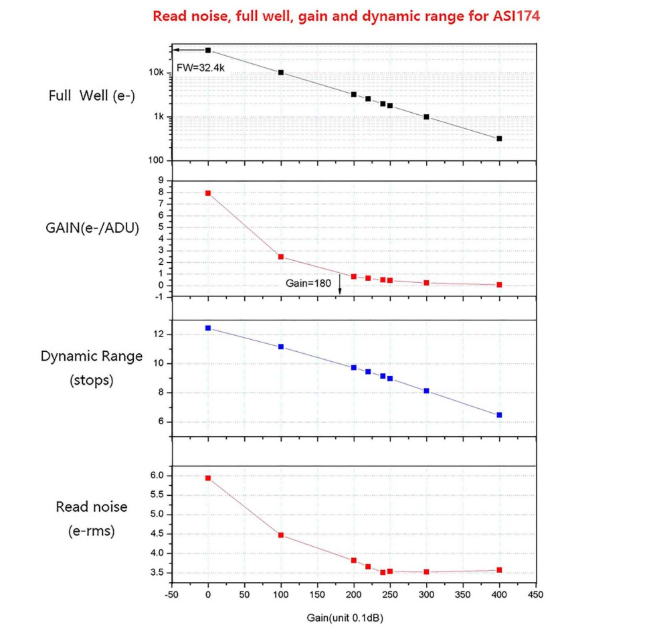
\includegraphics[width=0.78\textwidth]{figures/hw/cam_specs.png}
    \caption{Curvas de pozo completo, ganancia, rango dinámico y ruido de lectura reportadas para la cámara ASI174 en función de la ganancia de adquisición. \textbf{Fuente:} página oficial de ZWO (ZWO Astronomy Cameras).}
    \label{fig:camara-metricas-asi174}
\end{figure}

La Figura~\ref{fig:camara-metricas-asi174} complementa la selección de la cámara al mostrar cómo varían sus parámetros de operación con la ganancia. A ganancia baja, el sensor conserva una mayor capacidad de pozo completo, cercana a $32.4\,\mathrm{ke^-}$, y un rango dinámico superior a 12 pasos, condición favorable cuando se busca evitar saturación en regiones fotosféricas brillantes. Al incrementar la ganancia, la conversión en $\mathrm{e^-}/\mathrm{ADU}$ disminuye y el ruido de lectura se reduce hasta valores próximos a $3.5$--$4\,\mathrm{e^-_{rms}}$, pero también cae el pozo completo y el rango dinámico. Por ello, en el prototipo la ganancia debe elegirse como un compromiso: valores moderados permiten mejorar la sensibilidad aparente y la cadencia práctica, mientras que ganancias excesivas pueden limitar la capacidad de registrar simultáneamente detalles débiles y zonas brillantes sin saturación.

\subsection{Filtro solar y atenuación óptica}

En observación solar de luz blanca, la cuña de Herschel constituye una de las soluciones más eficaces para obtener una atenuación segura y una imagen de alto contraste en telescopios refractores, ya que desvía la mayor parte de la energía incidente fuera del eje óptico útil y deja pasar solo una fracción controlada hacia el sensor. Dado que la cámara seleccionada se integra en un tren óptico de 1.25\,$''$, la exploración del bloque de atenuación se restringe a cuñas de Herschel compatibles con ese diámetro. Bajo esta restricción, dejan de ser relevantes opciones de 2\,$''$ o filtros frontales de apertura completa, y el análisis se concentra en accesorios de 1.25\,$''$ que puedan acoplarse sin introducir adaptaciones innecesarias. Para mantener un criterio técnico comparable, la Tabla~\ref{tab:comparacion_filtros_proyecto} reúne características fundamentales de mercado: diámetro mecánico, presencia de filtrado integrado, compatibilidad con refractores y rasgos constructivos de interés para captura solar. El objetivo es contrastar cuñas de Herschel integrables dentro del mismo tren óptico de la cámara \citep{zwoASI174Manual2025,luntWhiteLightWedges2026,altairHerschelWedge2026,baaderHerschelUsage2026,apmLuntContinuum2026}.

\begin{table}[H]
\centering
\caption{Exploración de accesorios de atenuación solar compatibles con tren óptico de 1.25\,$''$. Los precios son referenciales y se expresan en dólares estadounidenses. \textbf{Fuente:} Elaboración propia.}
\label{tab:comparacion_filtros_proyecto}
\uniformtablestyle
\begin{tabularx}{\textwidth}{>{\raggedright\arraybackslash}p{3.35cm} >{\raggedright\arraybackslash}p{3.15cm} >{\centering\arraybackslash}p{1.45cm} X}
\toprule
\textbf{Fabricante / modelo} & \textbf{Característica técnica} & \textbf{Precio ref.} & \textbf{Observaciones} \\
\midrule
Altair Astro Solar Herschel Wedge 1.25\,$''$ & Variante de 1.25\,$''$ para refractores; orientada a imagen solar & US\$171 aprox. & Se destaca por su formato diagonal compacto y por una superficie cerámica pensada para disipación térmica. \\
Omegon Herschel Prism Tess 1.25\,$''$ & Filtro ND integrado; polarizador incorporado; rosca T2; compatibilidad 1.25\,$''$ & US\$229 & Se destaca por integrar conexión T2 para cámara y control de transmisión incorporado en la propia cuña. \\
Lunt Solar Systems White Light Solar Wedge 1.25\,$''$ & Filtro ND3 preinstalado; carcasa cerrada; trampa de luz integrada; uso en refractores hasta 4\,$''$ & US\$308 & Se destaca por ofrecer un sistema cerrado con trampa de luz interna y configuración lista para observación e imagen solar. \\
APM / Lunt Solar Wedge 1.25\,$''$ + Solar Continuum & ND3 preinstalado; filtro Solar Continuum incluido; uso en refractores & US\$345 aprox. & Se destaca por añadir un filtrado de contraste específico para realce fotosférico sobre la misma base óptica de Lunt. \\
\bottomrule
\end{tabularx}
\end{table}

Sobre esta base, el prototipo adopta la Lunt Solar Systems White Light Solar Wedge de 1.25\,$''$ como elemento principal de atenuación solar. La elección se apoya en un conjunto de rasgos funcionales que la distinguen dentro del grupo evaluado: filtro ND3 preinstalado, carcasa completamente cerrada, trampa de luz integrada y una orientación explícita del fabricante hacia observación e imagen solar en refractores. Estos elementos reducen luz parásita, simplifican la cadena óptica y dejan la cuña lista para uso seguro sin depender de accesorios adicionales para la atenuación primaria. Frente a opciones más económicas, Lunt ofrece una implementación más cerrada y directamente orientada a seguridad operacional; frente a configuraciones más costosas, como el paquete APM/Lunt con Solar Continuum, conserva la misma base óptica con menor complejidad y costo inicial \citep{luntWhiteLightWedges2026,altairHerschelWedge2026,apmLuntContinuum2026}.

\begin{figure}[H]
    \centering
    \begin{subfigure}[t]{0.47\textwidth}
        \centering
        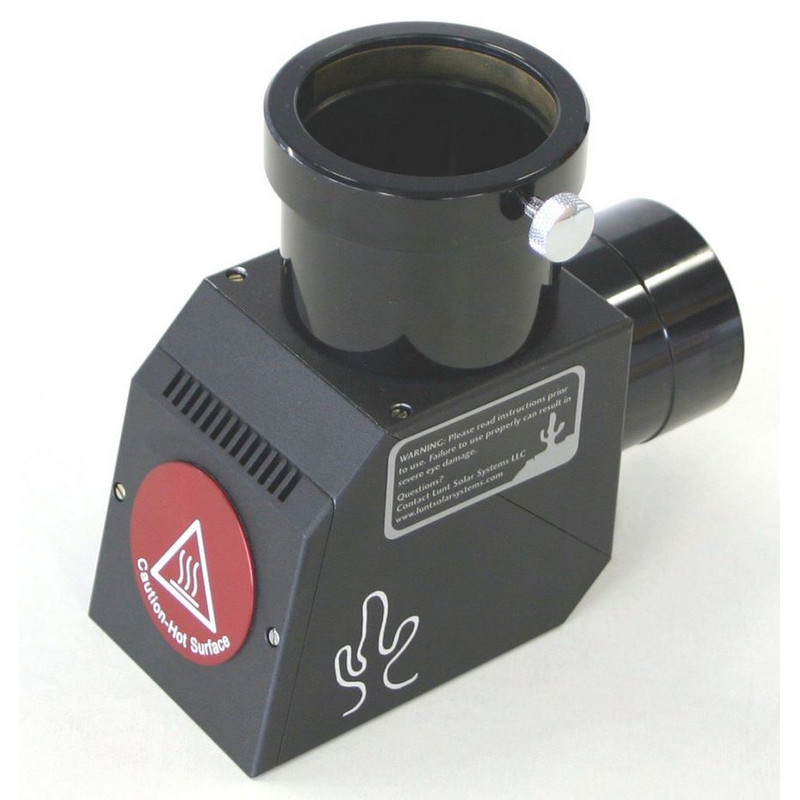
\includegraphics[width=\textwidth]{figures/hw/wedge.png}
        \caption{Prisma Herschel Lunt Solar Systems White Light Solar Wedge de 1.25\,$''$.}
    \end{subfigure}
    \hfill
    \begin{subfigure}[t]{0.40\textwidth}
        \centering
        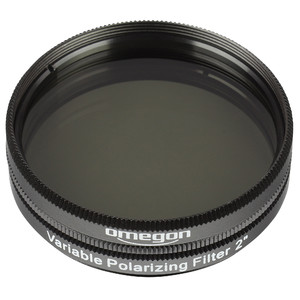
\includegraphics[width=\textwidth]{figures/hw/filter.png}
        \caption{Filtro ND3 interior del prisma.}
    \end{subfigure}
    \caption{Bloque de atenuación solar adoptado para el prototipo. Se muestran (a) el prisma Herschel Lunt de 1.25\,$''$ y (b) el filtro ND3 asociado al conjunto. \textbf{Fuente:} página oficial de Lunt Solar Systems.}
    \label{fig:herschel_project_filter}
\end{figure}

La documentación técnica insiste tanto en la presencia del filtro ND3 o del control de brillo asociado como en la prohibición de colocar filtros por delante de la cuña, precisamente por la carga térmica concentrada en ese punto del sistema \citep{luntWhiteLightWedges2026,altairHerschelWedge2026,baaderHerschelUsage2026}.

Como accesorio complementario, un polarizador puede emplearse después de la cuña para realizar un ajuste fino del brillo durante observación visual o captura. No obstante, su función es secundaria respecto del prisma de Herschel: la atenuación primaria y la seguridad óptica del sistema recaen en la cuña, mientras que la polarización solo modula la transmisión final según las condiciones de trabajo \citep{luntPolarizerWedge2026,baaderSinglePolarizer2026,baaderHerschelUsage2026}. 


\subsection{Plataforma de preprocesamiento y adquisición embebida}

Una vez definido el bloque instrumental, el siguiente componente es la plataforma
embebida encargada de coordinar la captura, ejecutar el preprocesamiento inicial,
almacenar temporalmente las observaciones y despachar la inferencia local. En
este trabajo, esta plataforma debe entenderse como la placa controladora de la
estación de observación, ya que concentra tanto la interacción con la cámara como
la lógica operativa del nodo en campo.

Desde el punto de vista funcional, la placa seleccionada debe reunir al menos
cuatro características. Primero, debe ofrecer capacidad suficiente de
procesamiento de imagen para controlar la cámara, ejecutar tareas de recorte,
normalización, compresión y validación básica de calidad, además de admitir
modelos ligeros de inferencia local. Segundo, debe soportar conectividad dual,
permitiendo operar tanto como cliente WiFi hacia una red disponible como en modo
\textit{hotspot} para configuración y monitoreo local cercano. Tercero, debe
mantener compatibilidad con distribuciones Linux estables, de preferencia Ubuntu
o Debian, para simplificar despliegue, mantenimiento y automatización. Cuarto,
debe ofrecer una ruta de integración práctica con el SDK de ZWO en entorno ARM,
de modo que la adquisición no dependa de software interactivo, sino de bibliotecas
programables \citep{nmcliHotspot2026,zwoASILinuxManual}.

Bajo estos criterios, la Tabla~\ref{tab:comparacion_plataformas_embebidas}
resume algunas opciones de mercado plausibles para una estación compacta de
adquisición solar \citep{raspberryPi5Docs2026,jetsonOrinNanoGuide2026,orangePi5Plus2026,rock5bDocs2026}.

\begin{table}[H]
\centering
\caption{Comparación de plataformas evaluadas para adquisición y preprocesamiento embebido en el prototipo. Los precios son referenciales y pueden variar según configuración, distribuidor y fecha de consulta. \textbf{Fuente:} Elaboración propia.}
\label{tab:comparacion_plataformas_embebidas}
\uniformtablestyle
\begin{tabularx}{\textwidth}{>{\raggedright\arraybackslash}p{2.65cm} >{\raggedright\arraybackslash}p{2.75cm} X >{\centering\arraybackslash}p{1.35cm} >{\raggedright\arraybackslash}p{2.55cm}}
\toprule
\textbf{Placa} & \textbf{Procesamiento de imagen} & \textbf{Características} & \textbf{Precio ref.} & \textbf{Observaciones} \\
\midrule
Raspberry Pi 5 (8 GB) & Broadcom BCM2712; CPU Cortex-A76 4 núcleos a 2.4 GHz; 8 GB LPDDR4X. & WiFi integrado doble banda; modo cliente/AP viable; alimentación 5 V, hasta 5 A. & US\$190 & Mejor equilibrio para estación portátil replicable. \\

NVIDIA Jetson Orin Nano & Arm Cortex-A78AE 6 núcleos; GPU Ampere 1024 CUDA; hasta 40 TOPS; 8 GB LPDDR5. & WiFi no integrado en módulo base; modo dual depende de adaptador; alimentación 19 V, aprox. 2.4 A en kit. & US\$249 & Mayor potencia, más costo y complejidad. \\

Orange Pi 5 Plus & RK3588; CPU 8 núcleos hasta 2.4 GHz; NPU 6 TOPS; 8--16 GB LPDDR4X. & WiFi no integrado; requiere módulo; modo dual depende del adaptador; alimentación 5 V, 4 A. & US\$149 & Buen rendimiento, integración menos directa. \\

ROCK 5B & RK3588; CPU 8 núcleos hasta 2.4 GHz; NPU 6 TOPS; 8--16 GB LPDDR4X. & WiFi no integrado; expansión M.2/E-key; modo dual depende del módulo; alimentación 5 V, hasta 5 A. & US\$145 & Potente, pero menos replicable. \\
\bottomrule
\end{tabularx}
\end{table}

A partir de esta comparación, se adopta la Raspberry Pi 5 en su variante de
8\,GB de RAM como placa controladora del sistema. La decisión no se fundamenta
únicamente en su capacidad de cómputo, suficiente para adquisición,
preprocesamiento e inferencia preliminar, sino también en su integración
inalámbrica nativa. Entre las alternativas evaluadas, es la opción que incorpora
WiFi de doble banda en la propia placa y permite una configuración práctica de
operación dual: punto de acceso local para control en campo y cliente de red para
sincronización de datos. Esta característica reduce adaptadores externos,
simplifica el montaje y mejora la portabilidad del prototipo. Además, la
disponibilidad de distribuciones Linux maduras y la integración efectiva con el
SDK de ZWO en entorno ARM reducen el riesgo de implementación y favorecen la
replicabilidad experimental \citep{raspberryPi5Docs2026,nmcliHotspot2026,zwoASILinuxManual}.


\begin{figure}[H]
    \centering
    \begin{subfigure}[t]{0.47\textwidth}
        \centering
        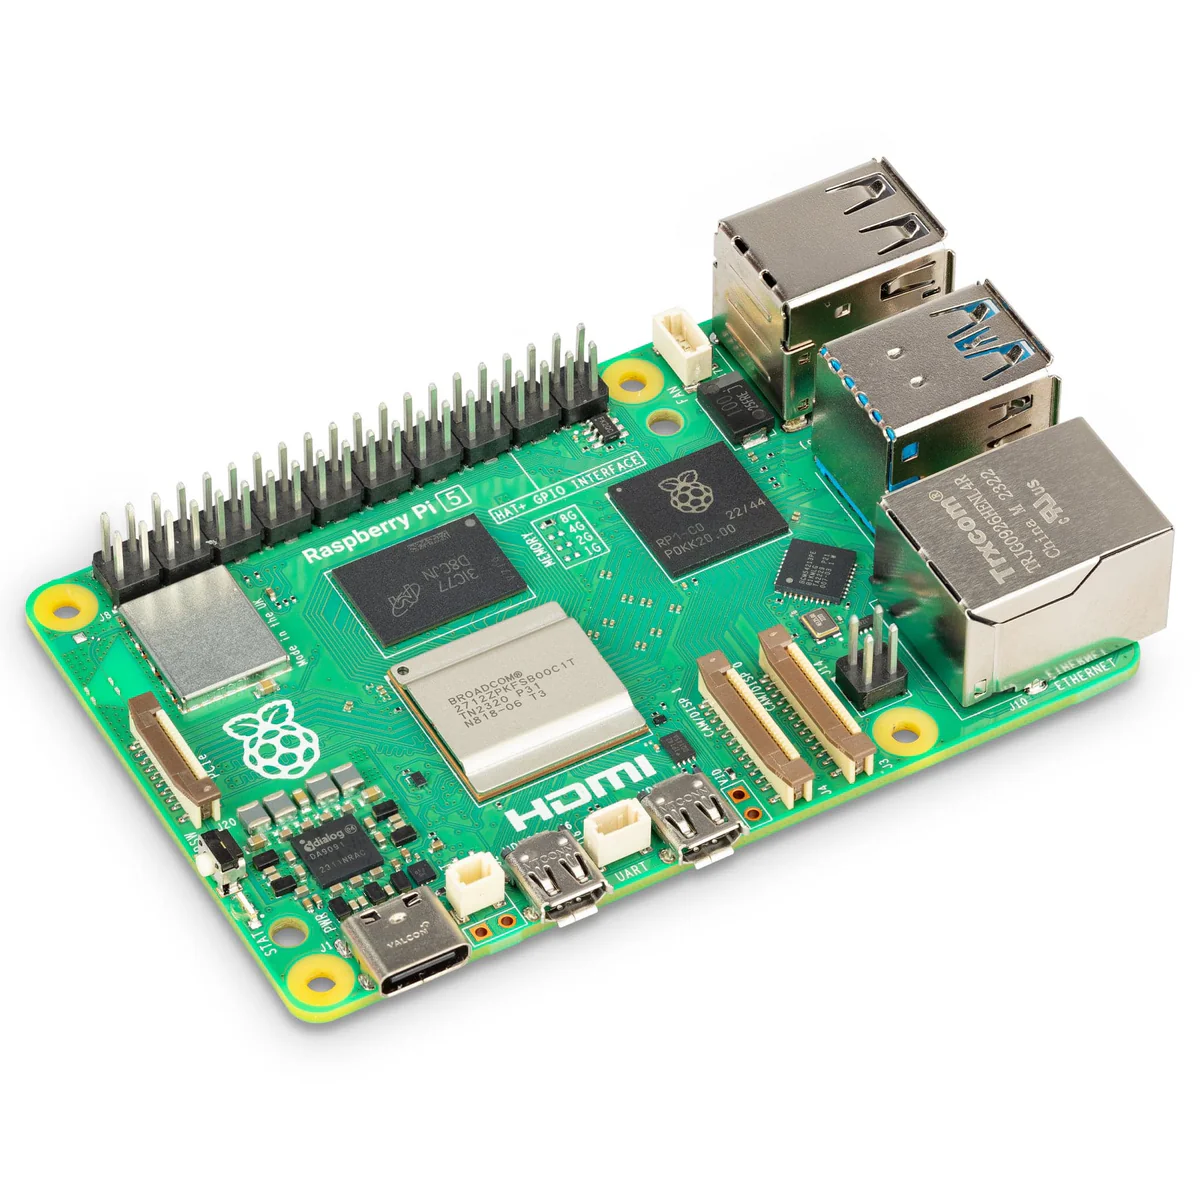
\includegraphics[width=\textwidth]{figures/hw/proc_unit.png}
        \caption{Imagen actual de la plataforma basada en Raspberry Pi 5.}
    \end{subfigure}
    \hfill
    \begin{subfigure}[t]{0.47\textwidth}
        \centering
        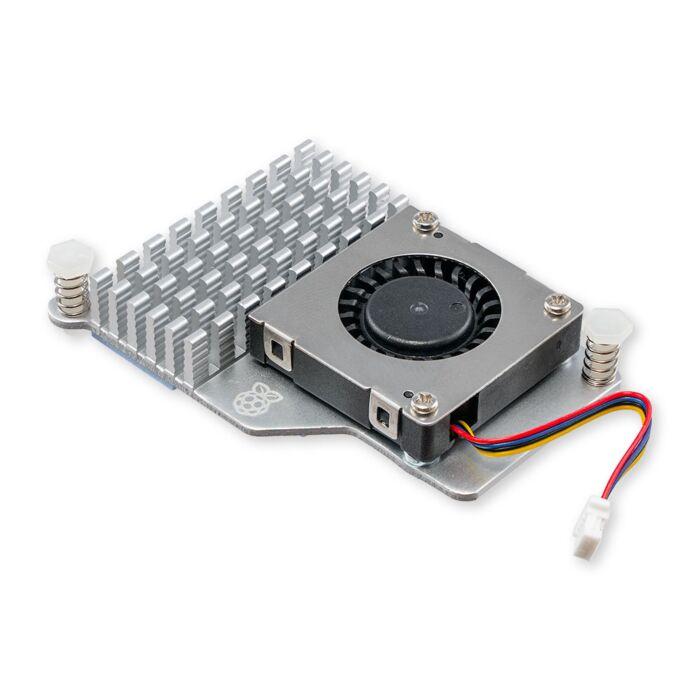
\includegraphics[width=\textwidth]{figures/hw/pi_cooler.jpg}
        \caption{\textit{Cooler} de disipación empleado sobre el procesador.}
    \end{subfigure}
    \caption{Plataforma embebida basada en Raspberry Pi 5 utilizada en el prototipo. Se muestran (a) la integración actual de la placa y (b) el sistema de disipación activa empleado para sostener operación continua en tareas de adquisición y preprocesamiento. \textbf{Fuente:} página oficial de Raspberry Pi.}
    \label{fig:rpi5_embebida_proyecto}
\end{figure}

A su vez, se emplea un
\textit{cooler} sobre el procesador para reducir el sobrecalentamiento y limitar
episodios de \textit{thermal throttling} durante sesiones prolongadas de
adquisición, preprocesamiento e inferencia. Esto resulta pertinente porque la
observación solar puede requerir secuencias continuas, transferencia de imágenes
y ejecución repetida de modelos, cargas que elevan la temperatura del chip.

\section{Procesamiento de imagen}

El procesamiento de imagen se organiza como una cadena modular que transforma
una imagen de disco solar completo en una recomendación taxonómica
Zurich--McIntosh. La Sección~\ref{sec:arquitectura-dl-cascada} describe el flujo
general de modelos y transformaciones entre etapas, mientras que la
Sección~\ref{sec:classification} formaliza la normalización bayesiana utilizada
para obtener la distribución final de recomendación.

\subsection{Arquitectura modular de Deep Learning en cascada}
\label{sec:arquitectura-dl-cascada}

\begin{figure}[H]
    \centering
    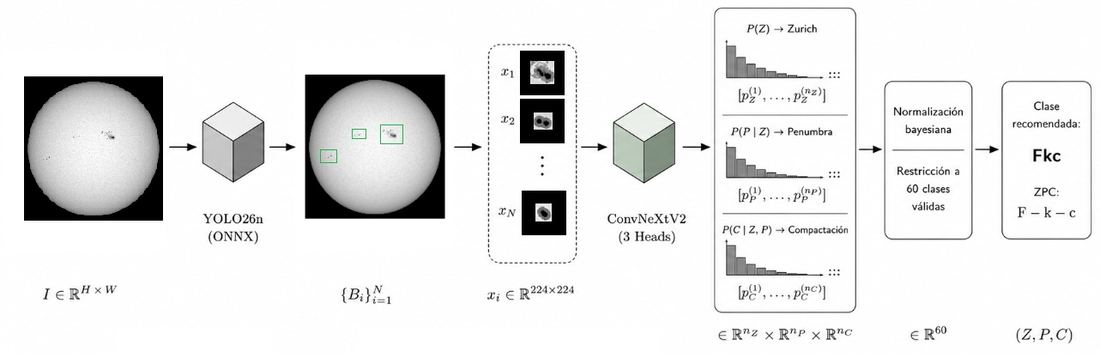
\includegraphics[width=1\textwidth]{figures/sys/img_pipe.jpg}
    \caption{Arquitectura modular en cascada para el procesamiento de imágenes solares. \textbf{Fuente:} Elaboración propia.}
    \label{fig:arquitectura-cascada-imagen}
\end{figure}

La Figura~\ref{fig:arquitectura-cascada-imagen} presenta la arquitectura de
procesamiento como una cascada de modelos y transformaciones intermedias. La primera etapa corresponde a la normalización geométrica de la imagen de disco
solar completo. En este nodo se centra el disco, se recorta la región útil y se
reescalan los datos a $640\times640$ píxeles. Esta salida constituye la entrada
del detector y reduce variaciones de escala y encuadre entre observaciones.

La segunda etapa corresponde a la detección con YOLO26n. El modelo identifica
regiones candidatas mediante \textit{bounding boxes}; cada caja representa un
grupo solar localizado sobre el disco. Esta etapa no asigna la clase
Zurich--McIntosh, sino que delimita las zonas que serán evaluadas por el
clasificador.

La tercera etapa transforma cada caja detectada en un recorte normalizado. Para
ello, la región delimitada se extrae de la imagen y se inserta en un lienzo de
$224\times224$ píxeles, preservando la relación de aspecto para evitar
distorsiones geométricas. El resultado es una colección de imágenes locales
homogéneas para la etapa de clasificación.

La cuarta etapa utiliza un clasificador jerárquico basado en ConvNeXtV2 Atto. Para
cada recorte, el backbone extrae una representación compacta y etapas MLP
complementarias inyectan la dependencia jerárquica entre los caracteres $Z$, $P$
y $C$ de la taxonomía Zurich--McIntosh. Estas salidas no constituyen todavía una
recomendación única, sino una representación probabilística separada por
componente, diseñada además para una conversión íntegra hacia ONNX.

La etapa final aplica normalización bayesiana sobre las salidas del
clasificador. En este bloque se combinan las probabilidades de $Z$, $P$ y $C$, se
anulan combinaciones taxonómicamente inválidas y se renormaliza la distribución
sobre las 60 clases admisibles. La clase con mayor probabilidad en este vector
final se toma como recomendación del sistema.

\subsection{Posprocesamiento con Normalización Bayesiana}

\label{sec:classification}

La dependencia semántica entre componentes se incorpora explícitamente mediante una formulación probabilística jerárquica que respeta la estructura observacional del esquema McIntosh. Para una imagen de entrada $x$, el objetivo es estimar la probabilidad conjunta de la tripleta $(Z,P,C)$, donde $Z$ representa el tipo de grupo, $P$ el carácter penumbral y $C$ la distribución interna del grupo. En su forma base, esta descomposición puede escribirse como
\begin{equation}
P(Z,P,C\mid x)=P(Z\mid x)\,P(P\mid Z,x)\,P(C\mid Z,P,x),
\end{equation}
lo que preserva la naturaleza jerárquica de la clasificación Zurich--McIntosh \citep{mcintosh1990classification}.

En la práctica, sin embargo, el modelo implementado produce tres salidas marginales para $Z$, $P$ y $C$ sin modelar de forma explícita todas las dependencias condicionales. Bajo esta aproximación operativa, se adopta
\begin{equation}
P(P\mid Z,x)\approx P(P\mid x),
\qquad
P(C\mid Z,P,x)\approx P(C\mid x),
\end{equation}
y por tanto se define una probabilidad base factorizada como
\begin{equation}
P_{\mathrm{base}}(Z,P,C\mid x)=P(Z\mid x)\,P(P\mid x)\,P(C\mid x).
\end{equation}
Esta construcción conserva la interpretabilidad del modelo multisalida y permite combinar las tres salidas dentro de una misma regla probabilística de recomendación.

Para imponer consistencia taxonómica se introduce una máscara binaria $M_{ZPC}\in\{0,1\}$, donde $M_{ZPC}=1$ si la combinación es válida dentro del esquema McIntosh y $M_{ZPC}=0$ en caso contrario. Con esta restricción se define la distribución truncada
\begin{equation}
\widetilde{P}(Z,P,C\mid x)=P_{\mathrm{base}}(Z,P,C\mid x)\,M_{ZPC},
\end{equation}
que anula combinaciones físicamente o taxonómicamente incompatibles. Para recuperar una distribución probabilística válida sobre el subconjunto de tripletas aceptadas, se aplica una renormalización bayesiana de la forma
\begin{equation}
P_{\mathrm{rec}}(Z,P,C\mid x)=
\frac{\widetilde{P}(Z,P,C\mid x)}{\sum_{z,p,c}\widetilde{P}(z,p,c\mid x)}
=
\frac{P_{\mathrm{base}}(Z,P,C\mid x)\,M_{ZPC}}{\sum_{z,p,c}P_{\mathrm{base}}(z,p,c\mid x)\,M_{zpc}},
\end{equation}
de modo que la masa total de probabilidad queda normalizada a uno sobre las combinaciones válidas. Esta reformulación permite interpretar $P_{\mathrm{rec}}$ como una distribución coherente para recomendación, ranking y análisis posterior.

La clase recomendada se obtiene entonces mediante
\begin{equation}
(Z^{\ast},P^{\ast},C^{\ast})=\arg\max_{Z,P,C} P_{\mathrm{rec}}(Z,P,C\mid x),
\end{equation}
y, si se desea una lectura secuencial compatible con el árbol de decisión, puede recuperarse además mediante marginalización jerárquica:
\begin{equation}
Z^{\ast}=\arg\max_{Z}\sum_{P,C}P_{\mathrm{rec}}(Z,P,C\mid x),
\qquad
P^{\ast}=\arg\max_{P}\sum_{C}P_{\mathrm{rec}}(Z^{\ast},P,C\mid x),
\end{equation}
\begin{equation}
C^{\ast}=\arg\max_{C}P_{\mathrm{rec}}(Z^{\ast},P^{\ast},C\mid x).
\end{equation}
Bajo esta formulación, la distribución recomendada no solo produce una etiqueta final, sino que también permite construir rankings top-$k$, cuantificar incertidumbre relativa entre clases vecinas y ofrecer una recomendación interpretable restringida al espacio válido de configuraciones \citep{sayez2023sunscc}.


\section{Formalización de modelos predictivos de la actividad solar}
\label{sec:forecast}

Este apartado formaliza el motor predictivo desarrollado para analizar la evolución del número de manchas solares y su migración latitudinal. El enfoque combina dos representaciones complementarias y produce dos series de salida: $\mathrm{SSN}_{\mathrm{PVLK}}$, obtenida a partir de un modelo escalar de Podladchikova--Van der Linden corregido con filtro de Kalman, y $\mathrm{SSN}_{\mathrm{DMD}}$, derivada directamente del modelo espacio-temporal aprendido mediante Descomposición en Modos Dinámicos (DMD) a partir de la vectorización temporal del diagrama de Spörer.

\subsection{Modelo PVL con filtro de Kalman adaptativo para el cálculo de SSN}

Para el pronóstico escalar se utiliza el modelo paramétrico de Podladchikova--Van der Linden como curva guía del ciclo solar. A diferencia del bloque DMD, que opera sobre vectores latitudinales $\mathbf{x}_t$, este bloque trabaja con un estado escalar. Para evitar ambigüedad de notación, se denota por $s_k\in\mathbb{R}$ el estado oculto correspondiente al SSN suavizado en el instante mensual $k$, y por $z_k\in\mathbb{R}$ la observación mensual disponible. La salida final de este bloque se denota como $\mathrm{SSN}_{\mathrm{PVLK}}$.

El perfil PVL proporciona una forma analítica base para la evolución esperada del ciclo solar. Sea $v$ el tiempo transcurrido, en meses, desde el inicio efectivo del ciclo. La función de forma se define como
\begin{equation}
f(v;a,b)=\frac{a v^{3}}{\exp\!\left(v^{2}/b^{2}\right)-0.71},
\end{equation}
donde $a$ controla la amplitud del ciclo y $b$ regula su anchura temporal. Para mantener una relación coherente con el efecto de Waldmeier, la escala temporal se vincula con la amplitud mediante la ley heurística
\begin{equation}
b(a)=27.12+25.15(1000a)^{-1/4}.
\end{equation}
En la implementación, el parámetro $a$ se ajusta iterativamente para que el máximo del perfil alcance una amplitud objetivo cercana a 140 unidades de SSN. Esta calibración fija una trayectoria base físicamente plausible, que luego se corrige con las observaciones mediante el filtro de Kalman.

La curva PVL se usa para construir el multiplicador de transición entre meses consecutivos. Dado el tiempo relativo $v_k$ asociado al instante $k$, se define
\begin{equation}
\Phi_k=\frac{f(v_k;a,b)}{f(v_{k-1};a,b)}.
\end{equation}
Este factor representa el cambio relativo esperado por la forma paramétrica del ciclo. Con ello, la etapa de predicción del filtro queda dada por
\begin{equation}
\widehat{s}_{k}^{-}=\Phi_k\widehat{s}_{k-1},
\end{equation}
\begin{equation}
P_k^{-}=\Phi_k^{2}P_{k-1}+Q_k,
\end{equation}
donde $\widehat{s}_{k}^{-}$ es la estimación a priori del SSN suavizado, $P_k^{-}$ es la varianza a priori y $Q_k$ es la varianza del ruido de proceso.

La etapa de actualización incorpora la observación $z_k$ mediante la ganancia de Kalman:
\begin{equation}
K_k=P_k^{-}\left(P_k^{-}+R_k\right)^{-1},
\end{equation}
\begin{equation}
\widehat{s}_{k}=\widehat{s}_{k}^{-}+K_k\left(z_k-\widehat{s}_{k}^{-}\right),
\end{equation}
\begin{equation}
P_k=(1-K_k)P_k^{-},
\end{equation}
donde $R_k$ es la varianza del ruido de medición. La innovación $z_k-\widehat{s}_{k}^{-}$ mide la discrepancia entre la observación mensual y la trayectoria esperada por el perfil PVL.

Para reflejar la heterocedasticidad del conteo de manchas solares, las varianzas de proceso y medición se escalan con la magnitud del estado predicho:
\begin{equation}
Q_k=0.2\,\widehat{s}_{k}^{-},
\end{equation}
\begin{equation}
R_k=2.5\,\widehat{s}_{k}^{-}.
\end{equation}
Este escalado permite que la incertidumbre aumente durante fases de mayor actividad y disminuya durante mínimos solares. La serie predictiva escalar queda finalmente definida como
\begin{equation}
\mathrm{SSN}_{\mathrm{PVLK}}(t_k)=\widehat{s}_{k}.
\end{equation}

\subsection{Vectorización temporal del diagrama de Spörer}

Para modelar el diagrama de Spörer, cada observación mensual se transforma en un vector de conteos latitudinales. Sea $N_{\mathrm{spots}}(t)$ el número total de manchas observadas en el instante $t$ y sea $\theta_i(t)$ la latitud heliográfica de la $i$-ésima mancha. El dominio latitudinal se restringe a
\begin{equation}
\theta \in [-50^{\circ},50^{\circ}],
\end{equation}
y se divide en $M=25$ contenedores de tamaño
\begin{equation}
\Delta \theta = 4^{\circ}.
\end{equation}

El $j$-ésimo contenedor se define como
\begin{equation}
\mathcal{B}_j=[\theta_j,\theta_{j+1}), \qquad j=1,\ldots,M.
\end{equation}
El conteo de manchas en dicho intervalo latitudinal se calcula mediante
\begin{equation}
V_j(t)=\sum_{i=1}^{N_{\mathrm{spots}}(t)}\mathbb{1}_{\mathcal{B}_j}\big(\theta_i(t)\big),
\end{equation}
donde $\mathbb{1}_{\mathcal{B}_j}$ es la función indicadora del contenedor $\mathcal{B}_j$. Con estos conteos, el estado latitudinal mensual queda dado por
\begin{equation}
\mathbf{x}_t=\begin{bmatrix}
V_1(t) & V_2(t) & \cdots & V_M(t)
\end{bmatrix}^{T}\in\mathbb{R}^{M}.
\end{equation}

La secuencia de $N$ observaciones mensuales se organiza en la matriz de snapshots
\begin{equation}
\mathbf{X}=\begin{bmatrix}
\mathbf{x}_1 & \mathbf{x}_2 & \cdots & \mathbf{x}_N
\end{bmatrix}\in\mathbb{R}^{M\times N}.
\end{equation}


\subsection{Modelo espacio-temporal del diagrama de Spörer con DMD}

La técnica DMD aproxima la evolución temporal mediante un operador lineal $\mathbf{A}$ que relaciona estados consecutivos. El modelo de un paso se expresa como
\begin{equation}
\mathbf{x}_{k+1}\approx\mathbf{A}\mathbf{x}_{k}.
\end{equation}
A partir de la matriz de snapshots se construyen dos matrices desplazadas
$\mathbf{X}_1$ y $\mathbf{X}_2$, formadas por estados consecutivos:
\begin{equation}
\mathbf{X}_1=\begin{bmatrix}
\mathbf{x}_1 & \mathbf{x}_2 & \cdots & \mathbf{x}_{N-1}
\end{bmatrix},
\qquad
\mathbf{X}_2=\begin{bmatrix}
\mathbf{x}_2 & \mathbf{x}_3 & \cdots & \mathbf{x}_{N}
\end{bmatrix},
\end{equation}
con $\mathbf{X}_1,\mathbf{X}_2\in\mathbb{R}^{M\times(N-1)}$. El operador se
estima mediante una descomposición en valores singulares truncada de rango
$r=10$:
\begin{equation}
\mathbf{X}_1\approx\mathbf{U}_r\boldsymbol{\Sigma}_r\mathbf{V}_r^{H}.
\end{equation}
El operador reducido en la base dominante queda definido por $\tilde{\mathbf{A}}=\mathbf{U}_r^{H}\mathbf{X}_2\mathbf{V}_r\boldsymbol{\Sigma}_r^{-1}$, mientras que el operador de rango completo se reconstruye como
\begin{equation}
\mathbf{A}\approx\mathbf{X}_2\mathbf{V}_r\boldsymbol{\Sigma}_r^{-1}\mathbf{U}_r^{H}.
\end{equation}

Con este operador, la reconstrucción histórica de un paso se obtiene mediante $\widehat{\mathbf{x}}_{k}=\mathbf{A}\mathbf{x}_{k-1}$ ($k\leq N$), mientras que la proyección futura se calcula iterativamente como
\begin{equation}
\widehat{\mathbf{x}}_{k+1}=\mathbf{A}\widehat{\mathbf{x}}_{k}, \qquad k>N.
\end{equation}

\subsubsection{SSN calculado como integral discreta del modelo espacio-temporal}

El índice global reconstruido desde DMD se obtiene integrando la distribución latitudinal predicha. En este caso, la salida primaria del modelo no es una serie escalar, sino el vector de estado predicho $\widehat{\mathbf{x}}_t$, consistente con la notación definida para los snapshots latitudinales:
\begin{equation}
\widehat{\mathbf{x}}_t=\begin{bmatrix}
\widehat{V}_1(t) & \widehat{V}_2(t) & \cdots & \widehat{V}_M(t)
\end{bmatrix}^{T}.
\end{equation}
El número de manchas solares asociado al modelo DMD, $\mathrm{SSN}_{\mathrm{DMD}}$, se deriva directamente de ese vector mediante la suma calibrada de sus componentes:
\begin{equation}
\mathrm{SSN}_{\mathrm{DMD}}(t)=\kappa\sum_{j=1}^{M}\widehat{V}_j(t),
\end{equation}
donde $\kappa$ calibra la suma latitudinal respecto a la escala histórica:
\begin{equation}
\kappa=\frac{\sum_{t=1}^{N}\mathrm{SSN}_{\mathrm{obs}}(t)}{\sum_{t=1}^{N}\sum_{j=1}^{M}\widehat{V}_j(t)}.
\end{equation}
 
\chapter[Diseño del hardware]{Diseño del hardware\label{cap:hardware}}

El hardware del prototipo se organiza como una estación compacta de
observación solar, con operación local y sincronización remota. La
Raspberry Pi 5 concentra las funciones de control, adquisición,
preprocesamiento y comunicación, mientras que la cámara ZWO ASI174MM Mini y el
prisma Herschel wedge con filtro ND3.0 conforman el bloque óptico para captura
fotosférica en luz blanca.

La arquitectura integra cámara, pantalla local de estado, refrigeración activa,
conectividad inalámbrica y almacenamiento temporal en un nodo embebido único.
Esta disposición permite operar el instrumento aun sin conexión permanente a
Internet y reservar la sincronización con la plataforma web para los periodos en
que el enlace esté disponible. La Figura~\ref{fig:esquema_electrico_general_hardware}
resume la integración eléctrica entre la Raspberry Pi 5 y los elementos
principales del prototipo.

\begin{figure}[H]
    \centering
    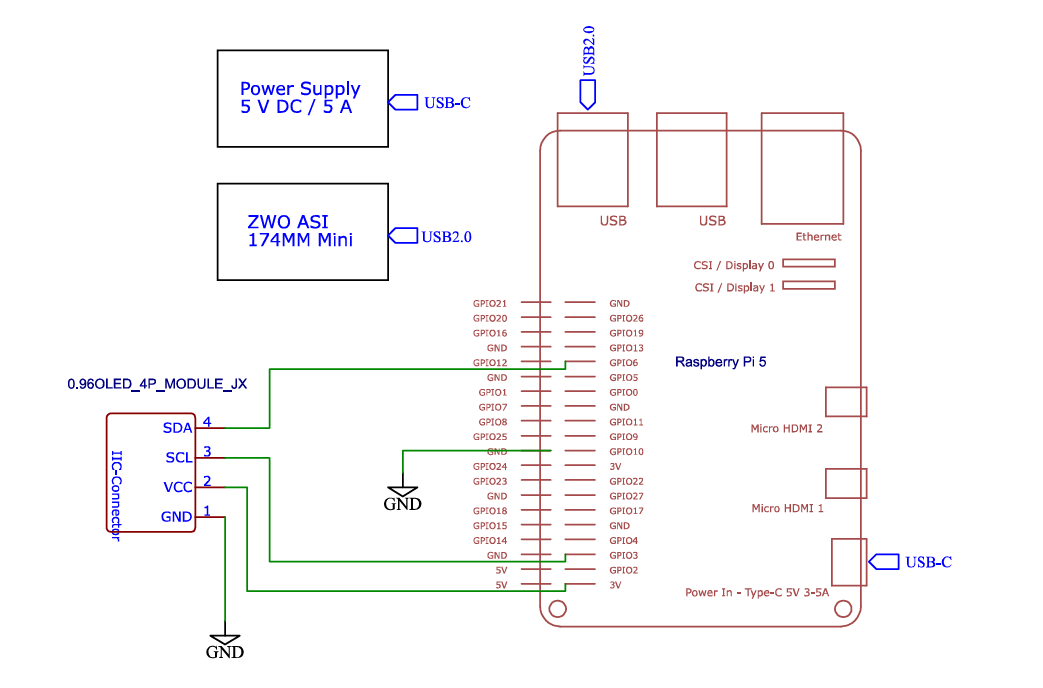
\includegraphics[width=0.90\textwidth]{figures/hw/electric.png}
    \caption{Esquema eléctrico general del sistema de adquisición, mostrando la
    Raspberry Pi 5 como unidad central. \textbf{Fuente:} Elaboración propia.}
    \label{fig:esquema_electrico_general_hardware}
\end{figure}

\section{Unidad de procesamiento embebido}

La implementación adopta una Raspberry Pi 5 de 8\,GB como unidad de
procesamiento embebido, en concordancia con los criterios de selección expuestos
en la Tabla~\ref{tab:comparacion_plataformas_embebidas}. Esta placa cumple el rol
de nodo de borde (\textit{edge computing}): inicializa los servicios de
adquisición, gestiona la cámara, ejecuta el preprocesamiento local y almacena de
forma temporal capturas, metadatos e inferencias preliminares.

La conectividad combina un punto de acceso local mediante \textit{hotspot}, para
configuración y monitoreo en campo, con enlace WiFi hacia una red disponible para
sincronización posterior con la plataforma web y la base de datos en la nube
\cite{raspberryPi5Docs2026,nmcliHotspot2026}. Debido a la ejecución continua de
adquisición, transferencia y preprocesamiento, se incorpora refrigeración activa
(\textit{active cooler}) para mejorar la disipación térmica y reducir eventos de
\textit{thermal throttling} durante sesiones prolongadas.

\begin{figure}[H]
    \centering
    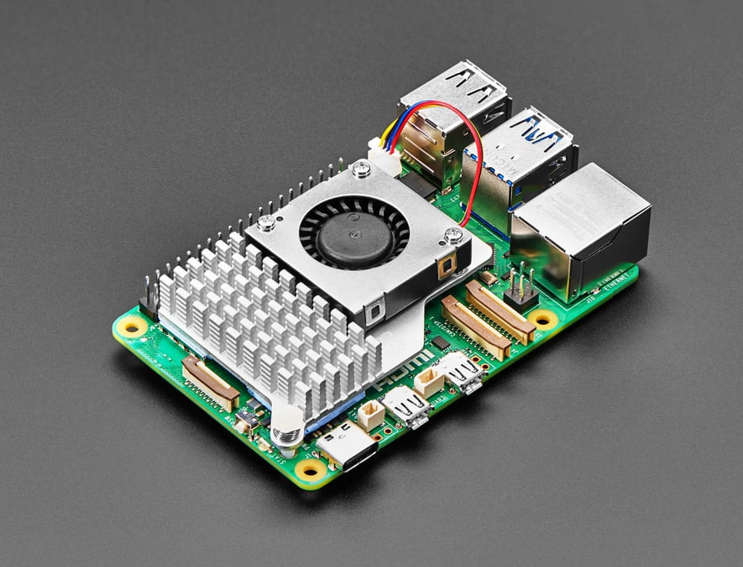
\includegraphics[width=0.70\textwidth]{figures/hw/cooler.png}
    \caption{Raspberry Pi 5 de 8\,GB con sistema de refrigeración activa,
    empleada como unidad de procesamiento embebido para captura,
    preprocesamiento local, inferencia preliminar y sincronización con la nube. \textbf{Fuente:} página oficial de Raspberry Pi.}
    \label{fig:raspberry_pi5_nodo_borde}
\end{figure}

\subsection{Pantalla local de estado}

Como interfaz auxiliar se emplea una pantalla OLED de \(0.96''\) y resolución
\(128\times64\) píxeles. Su función es entregar diagnóstico inmediato en campo:
estado de red, disponibilidad del \textit{hotspot}, detección de cámara,
ejecución del servicio de adquisición y avisos básicos de error. De este modo, el
operador puede verificar el estado del nodo sin recurrir a un monitor externo,
una sesión SSH ni la plataforma web.

La comunicación con la Raspberry Pi 5 se realiza mediante bus I2C, reduciendo la
interconexión a dos líneas de datos/control y dos líneas de alimentación. La
Tabla~\ref{tab:conexionado_oled_pi5} resume el conexionado empleado.

\begin{figure}[H]
    \centering
    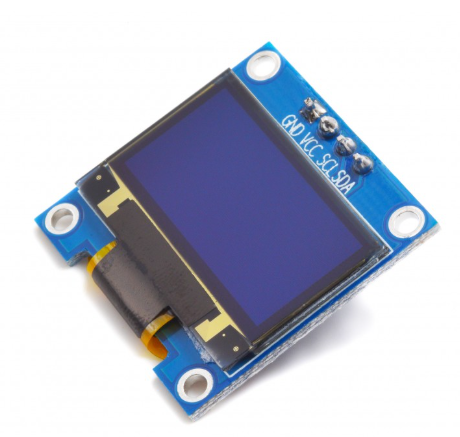
\includegraphics[width=0.55\textwidth]{figures/hw/oled.png}
    \caption{Pantalla OLED compacta de \(0.96''\) y resolución de
    \(128\times64\) píxeles empleada para mostrar el estado de conectividad,
    detección de cámara y ejecución de servicios locales. \textbf{Fuente:} JLCPCB.}
    \label{fig:oled_128x64_estado}
\end{figure}

\begin{table}[H]
    \centering
    \caption{Conexionado de la pantalla OLED \(128\times64\) con la Raspberry Pi 5 mediante I2C. \textbf{Fuente:} Elaboración propia.}
    \label{tab:conexionado_oled_pi5}
    \begin{tabular}{lll}
        \hline
        \textbf{Pin OLED} & \textbf{Pin físico Raspberry Pi 5} & \textbf{Función} \\
        \hline
        VCC & Pin 1 & Alimentación de 3.3V \\
        GND & Pin 6 & Tierra común del sistema \\
        SCL & Pin 5 / GPIO3 & Línea de reloj I2C \\
        SDA & Pin 3 / GPIO2 & Línea de datos I2C \\
        \hline
    \end{tabular}
\end{table}

\subsection{Diseño 3D de protección}

Se desarrolló una carcasa en SolidWorks 2022 para proteger la Raspberry Pi 5 y
sus elementos asociados durante montaje, transporte y operación. El diseño cubre
zonas sensibles de la placa sin obstruir los accesos de alimentación, cámara,
pantalla, red y mantenimiento.

La geometría incorpora aberturas y holguras compatibles con el sistema de
refrigeración activa, preservando el flujo de aire alrededor del disipador y del
ventilador. Además, define posiciones fijas para la placa, la pantalla y el paso
de cables, lo que mejora la repetibilidad del montaje y facilita la inspección o
reemplazo de componentes.

\begin{figure}[H]
    \centering
    \begin{subfigure}[t]{0.48\textwidth}
        \centering
        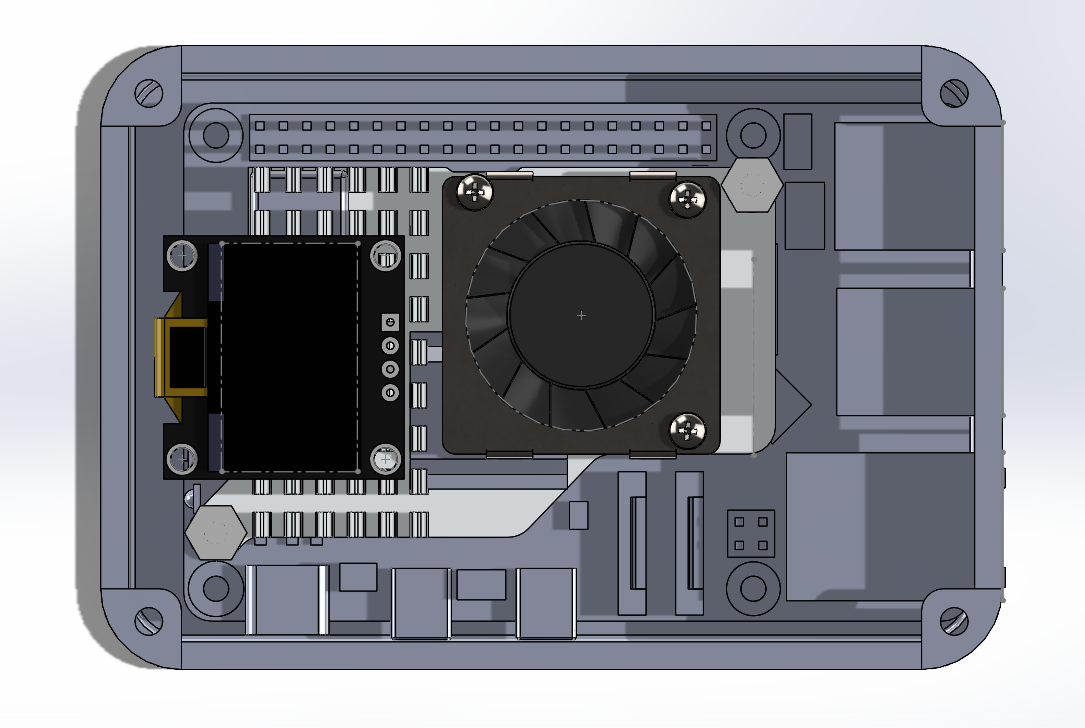
\includegraphics[width=\textwidth]{figures/cad/case_open.png}
        \caption{Vista de la carcasa sin tapa, mostrando el volumen interno y
        las zonas previstas para alojamiento de componentes.}
    \end{subfigure}
    \hfill
    \begin{subfigure}[t]{0.48\textwidth}
        \centering
        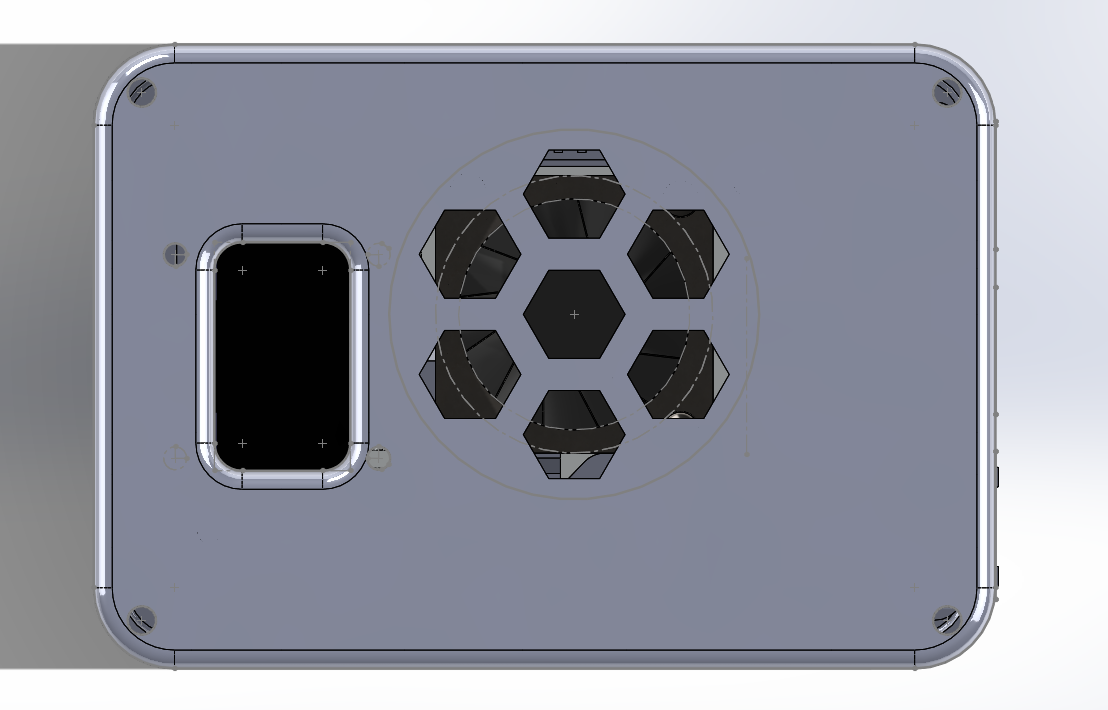
\includegraphics[width=\textwidth]{figures/cad/case_lid.png}
        \caption{Vista de la tapa de cierre diseñada para proteger el conjunto
        sin bloquear la ventilación ni los accesos principales.}
    \end{subfigure}
    \caption{Diseño 3D de la carcasa de protección desarrollado en SolidWorks
    2022. Se muestran (a) el cuerpo principal sin tapa y (b) la tapa del conjunto
    de protección. \textbf{Fuente:} Elaboración propia.}
    \label{fig:diseno_3d_proteccion_pi5}
\end{figure}

\section{Sistema de captura}

El sistema de captura integra el telescopio refractor, la cámara monocromática,
el elemento de atenuación solar y la interfaz de control ejecutada en la
Raspberry Pi 5. Su función es obtener imágenes fotosféricas en luz blanca,
almacenarlas localmente y dejarlas disponibles para preprocesamiento, inferencia
y sincronización posterior.

\subsection{Configuración de firmware}

La adquisición se implementa en Ubuntu~24 mediante el SDK de ZWO para cámaras
ASI sobre Raspberry Pi 5. Esta interfaz permite controlar por software la
exposición, ganancia, formato de imagen, región de interés y secuencias de
captura, evitando la operación manual durante la adquisición
\cite{zwoASILinuxManual,raspberryPi5Docs2026}.

La configuración de bajo nivel parte de verificar la arquitectura del sistema y
seleccionar la biblioteca compartida correspondiente del SDK. En una estación de
desarrollo x64 se utiliza la biblioteca de escritorio; en Raspberry Pi 5 se usa
la variante ARM compatible, típicamente la carpeta \texttt{armv8}. Esta distinción
es crítica porque la cámara se inicializa mediante \texttt{libASICamera2.so}; una
biblioteca compilada para otra arquitectura impediría abrir el dispositivo.

\begin{lstlisting}[language=bash,basicstyle=\footnotesize\ttfamily,breaklines=true,caption={Verificación de arquitectura y selección de biblioteca del SDK de ZWO.},label={lst:zwo-arquitectura}]
uname -m
ls SDK_ZWO/lib
# En Raspberry Pi 5 se selecciona la variante ARM compatible.
# Ejemplo: armv8.
\end{lstlisting}

Instalada la biblioteca, el entorno de ejecución se configura mediante
\texttt{ZWO\_ASI\_LIB}, variable que apunta a \texttt{libASICamera2.so} y permite
que los módulos basados en \texttt{zwoasi} localicen el controlador sin rutas
codificadas en el programa. Además, se actualiza la caché del sistema mediante
\texttt{ldconfig} para dejar la biblioteca disponible a los servicios de captura.

\begin{lstlisting}[language=bash,basicstyle=\footnotesize\ttfamily,breaklines=true,caption={Configuración de la biblioteca compartida del SDK de ZWO.},label={lst:zwo-biblioteca}]
export ZWO_ASI_LIB=ruta/del/sdk/armv8/libASICamera2.so
echo "ZWO_ASI_LIB=$ZWO_ASI_LIB"
ldconfig -v | grep ASICamera
\end{lstlisting}

También se incorpora una regla \texttt{udev} para el identificador USB del
fabricante ZWO, asociado al \texttt{idVendor} \texttt{03c3}. Esta regla asigna
permisos de acceso al dispositivo USB y evita que la captura dependa de ejecutar
el servicio con privilegios administrativos. En la práctica, el proceso de
arranque verifica la presencia de la cámara mediante detección USB, carga el SDK,
abre la comunicación con la ASI174MM Mini y solo entonces habilita las rutinas de
configuración de exposición, ganancia, formato de imagen y región de interés.

\begin{lstlisting}[language=bash,basicstyle=\footnotesize\ttfamily,breaklines=true,caption={Regla \texttt{udev} mínima para cámaras ZWO ASI.},label={lst:zwo-udev}]
SUBSYSTEM=="usb", ATTR{idVendor}=="03c3", \
  MODE="0666", GROUP="plugdev"
udevadm control --reload-rules
udevadm trigger
\end{lstlisting}

Sobre esta base se instalan las dependencias necesarias para captura y análisis
local: \texttt{zwoasi} para acceder al SDK, \texttt{opencv-python} para
operaciones de imagen, \texttt{numpy} para manejo matricial y \texttt{ultralytics}
cuando se requiere inferencia YOLO en el entorno de pruebas. Estas dependencias completan la configuración funcional del nodo al permitir detección de cámara, captura de imágenes y
generación de metadatos para la plataforma.

\begin{lstlisting}[language=bash,basicstyle=\footnotesize\ttfamily,breaklines=true,caption={Instalación de dependencias de adquisición y análisis local.},label={lst:zwo-dependencias}]
python -m pip install zwoasi opencv-python numpy ultralytics
python - <<'EOF'
import zwoasi as asi
print("SDK ZWO disponible")
EOF
\end{lstlisting}

\subsection{Captura de imagen}

El núcleo técnico del sistema es la transferencia eficiente de datos desde el
SDK nativo de ZWO hacia el flujo de procesamiento basado en \texttt{OpenCV}. Esta
capa organiza la lectura del sensor, la transferencia USB~2.0 y la conversión de
los datos crudos en matrices compatibles con visión artificial.

El proceso se ejecuta mediante un hilo especializado, de desarrollo propio,
\texttt{CameraWorker}, que opera como puente asíncrono entre la cámara y las
capas superiores del sistema. La adquisición invoca métodos de bajo nivel del SDK
para recuperar buffers crudos desde el bus USB~2.0. Estos buffers contienen la
información digitalizada por el sensor en formatos como RAW8 o RGB24,
inicialmente representada como flujos lineales de bytes.

La integración con \texttt{OpenCV} se realiza mediante \texttt{NumPy}. El buffer
se interpreta con \texttt{frombuffer} como una matriz unidimensional y luego se
reestructura mediante \textit{reshaping} según las dimensiones de la región de
interés (ROI). Así, el flujo binario se convierte en un \texttt{ndarray}
compatible con codificación, filtrado y análisis de imagen.

Para mantener una respuesta adecuada durante vista previa, enfoque y verificación
de exposición, las operaciones se ejecutan sobre datos residentes en memoria,
evitando escrituras intermedias en disco. Además, la adquisición concurrente
permite que \texttt{CameraWorker} mantenga el ciclo de captura mientras el backend
realiza compresión JPEG en tiempo real, generando datos optimizados para
transmisión y visualización local sin interrumpir la lectura del sensor.

\section{Conectividad y configuración de red local}
\label{sec:conectividad-hardware}

La robustez operativa en campo depende de una conectividad dual que no interfiera
con la adquisición. Para ello, la Raspberry Pi 5 opera como cliente de una red
externa y, simultáneamente, como punto de acceso inalámbrico para control local.
La interfaz \texttt{wlan0} se reserva para la conexión WiFi disponible, mientras
que la interfaz virtual \texttt{ap0} se dedica a la red privada del instrumento.

Esta separación permite acceso directo al prototipo aun sin Internet y mantiene
la posibilidad de sincronizar datos cuando la red externa esté disponible. La red
local se orienta al control inmediato, monitoreo y acceso al panel de operación;
la conexión externa se reserva para transferencia diferida, respaldo y consulta
remota de resultados.

La gestión del punto de acceso se realiza mediante \texttt{hostapd}. En esta
configuración se emplea el controlador \texttt{nl80211}, encargado de la
comunicación con el subsistema inalámbrico de Linux y el chip de radio de la
Raspberry Pi 5. El siguiente bloque resume los parámetros utilizados para
establecer la red privada del instrumento.

\begin{lstlisting}[language=bash,basicstyle=\footnotesize\ttfamily,breaklines=true,caption={Configuración del punto de acceso local mediante hostapd.},label={lst:hostapd-ap0}]
interface=ap0
driver=nl80211
ssid=Pi5_Observatory_Local
hw_mode=g
channel=11
wmm_enabled=1
macaddr_acl=0
auth_algs=1
ignore_broadcast_ssid=0
wpa=2
wpa_passphrase=Observatory2026
wpa_key_mgmt=WPA-PSK
wpa_pairwise=TKIP
rsn_pairwise=CCMP

# Stability optimizations
ieee80211n=1
# Optimized HT40 caps for channel compatibility
ht_capab=[SHORT-GI-20][DSSS_CCK-40]
\end{lstlisting}

Para automatizar la comunicación de los dispositivos conectados se emplea
\texttt{dnsmasq} como servicio local de DHCP y resolución de nombres. Este
componente asigna direcciones IP en la subred privada y resuelve el dominio local
asociado al panel de control, evitando que el operador deba recordar una dirección
IP específica.

La configuración se restringe a \texttt{ap0} para evitar interferencias con otras
interfaces de red. Además, define un rango DHCP acotado y establece la Raspberry
Pi 5 como puerta de enlace y servidor DNS. El dominio \texttt{observatory.local}
se resuelve hacia la dirección fija del nodo de control, facilitando el acceso al
backend y al panel local.

\begin{lstlisting}[language=bash,basicstyle=\footnotesize\ttfamily,breaklines=true,caption={Configuración de dnsmasq para asignación DHCP y resolución local.},label={lst:dnsmasq-ap0}]
# Only listen on the AP interface
interface=ap0
bind-dynamic

# DHCP Range (192.168.4.10 to 192.168.4.100)
dhcp-range=192.168.4.10,192.168.4.100,255.255.255.0,24h

# DHCP Options (3=Gateway, 6=DNS)
dhcp-option=3,192.168.4.1
dhcp-option=6,192.168.4.1

# Optimization for low latency
domain-needed
bogus-priv
no-resolv
local=/observatory.local/
address=/observatory.local/192.168.4.1
\end{lstlisting}

En conjunto, esta infraestructura permite que el nodo de observación funcione de
forma autónoma en campo. El operador accede mediante la red local y el dominio
\texttt{observatory.local} para controlar la captura y revisar servicios sin
conexión externa. Cuando existe Internet, la interfaz destinada a redes externas
habilita la sincronización diferida con la plataforma web sin comprometer el
enlace local de operación. 
\chapter[Diseño del software]{Diseño del software\label{cap:software}}

El software del prototipo se diseña como una cadena integrada de adquisición,
análisis, persistencia y visualización. A partir de imágenes solares y reportes
observacionales históricos se construyen conjuntos de entrenamiento trazables;
sobre ellos se entrena una arquitectura en cascada de inteligencia artificial para localizar y
clasificar regiones activas; los resultados se complementan con modelos
predictivos de evolución temporal; finalmente, la información generada se
almacena en una base de datos relacional y se expone mediante una plataforma web.

Esta organización mantiene una separación clara entre las funciones de
entrenamiento, inferencia, predicción y consulta, pero las conecta mediante los
mismos identificadores, fechas de observación, metadatos y otros elementos derivados.
De este modo, cada captura puede seguirse desde su origen visual hasta su
clasificación, almacenamiento y presentación.

\section{Datos de entrenamiento}

\label{sec:data-software}

Los datos de entrenamiento se obtienen a partir de dos fuentes
complementarias: imágenes de disco solar completo provenientes de SDO/HMI y
reportes diarios NOAA SRD, sigla utilizada para referirse a \textit{Solar Region
Summary}, correspondientes al período de 2010 al 2025
\citep{scherrer2012hmi,noaaSRS}. El acoplamiento entre ambas fuentes asocia,
para cada fecha, la evidencia visual del disco solar con la información
descriptiva de las regiones activas reportadas, incluyendo posición,
identificación NOAA y descriptores morfológicos. Esta fusión imagen--metadatos
permite generar etiquetas consistentes, trazables y útiles para entrenamiento
supervisado.

Aunque el sistema final está orientado a operar con imágenes en luz blanca, la
etapa de entrenamiento se apoyó en el acoplamiento HMI--SRD debido a que todos
los registros considerados corresponden a observaciones diarias de las
00:30~UTC. No se utilizaron capturas en luz blanca del SIDC para construir las
etiquetas de entrenamiento, ya que dicho repositorio no dispone de imágenes
sistemáticas en ese horario. La decisión es razonable desde el punto de vista
morfológico: ambas modalidades representan la fotosfera y muestran las manchas
solares como estructuras oscuras sobre el disco. La
Figura~\ref{fig:hmi-white-light-comparison} ilustra esta correspondencia visual
\citep{scherrer2012hmi,bobra2014sharp,zhou2023mcintosh,noaaSRS}.

\begin{figure}[H]
    \centering
    \begin{subfigure}[t]{0.47\textwidth}
        \centering
        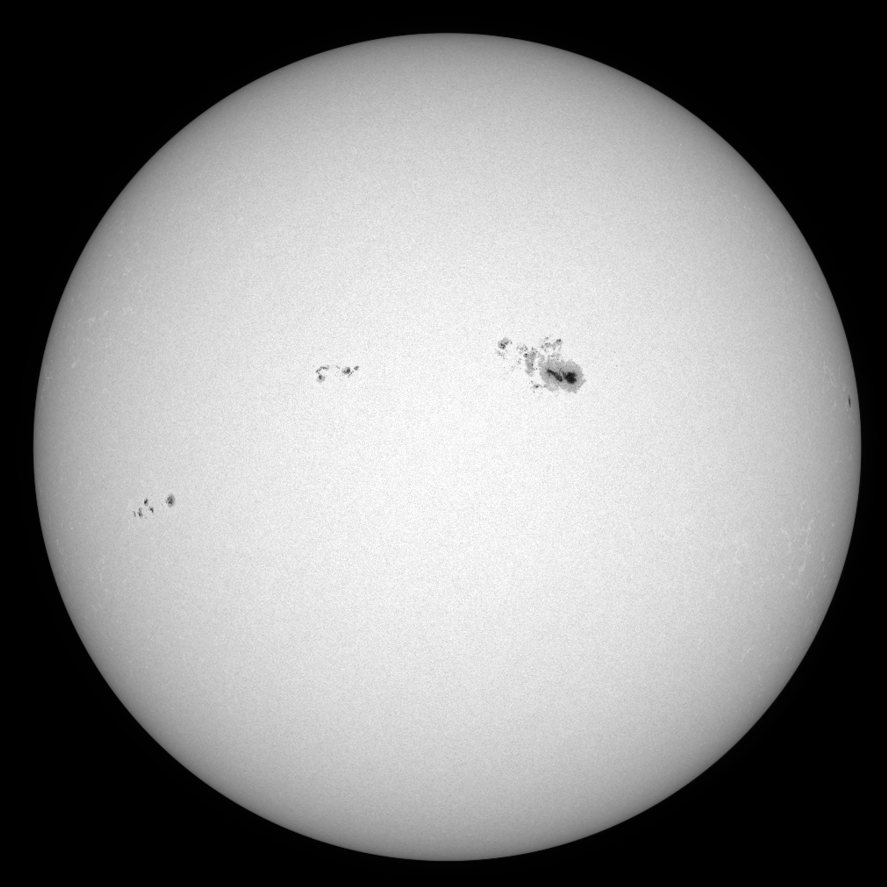
\includegraphics[width=\textwidth]{figures/data/hmi.png}
        \caption{Imagen HMI.}
    \end{subfigure}
    \hfill
    \begin{subfigure}[t]{0.47\textwidth}
        \centering
        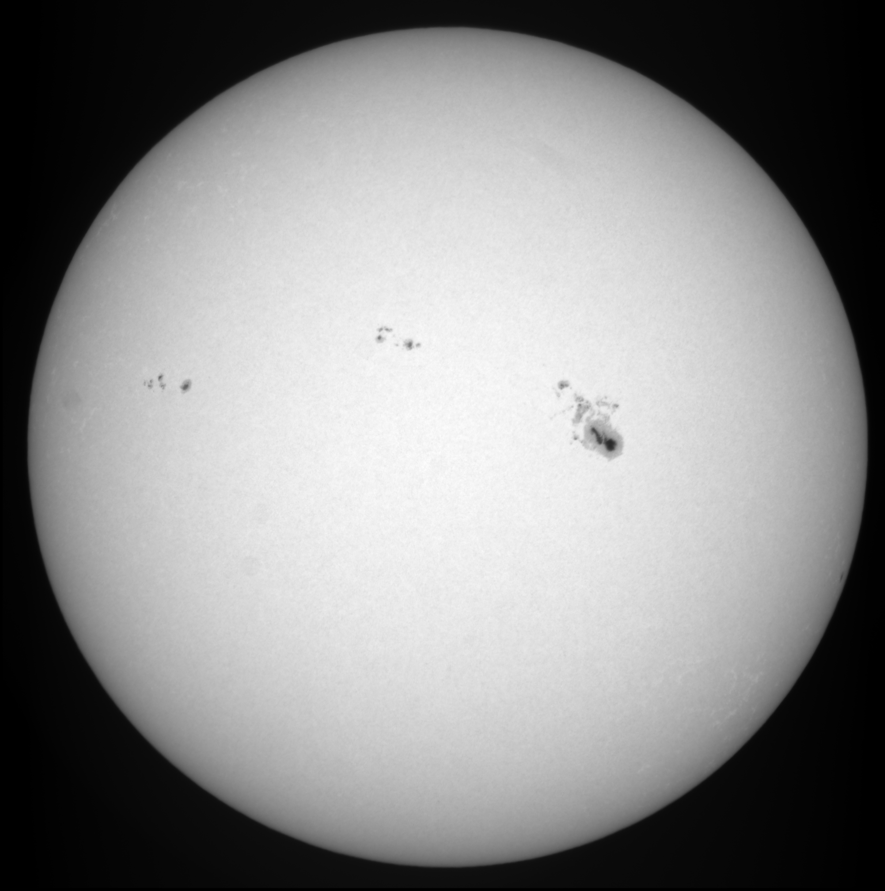
\includegraphics[width=\textwidth]{figures/data/wl.png}
        \caption{Imagen luz blanca.}
    \end{subfigure}
    \caption{Comparación visual entre modalidades fotosféricas de disco completo
    para la fecha 05-06-2025. La subfigura (a) corresponde a una imagen HMI
    obtenida por SDO/NASA, mientras que la subfigura (b) corresponde a una imagen
    luz blanca del SIDC del Royal Observatory of Belgium. \textbf{Fuente:} Elaboración propia a partir de imágenes SDO/NASA y SIDC.}
    \label{fig:hmi-white-light-comparison}
\end{figure}

\subsection{Transferencia de dominio y acoplamiento SDO--NOAA}

La transferencia de dominio se plantea como una estrategia para construir
etiquetas de entrenamiento a partir de fuentes observacionales complementarias.
Las imágenes SDO/HMI aportan una representación fotosférica uniforme del disco
solar completo, mientras que los reportes diarios NOAA SRD proporcionan la
identificación de regiones activas, sus coordenadas heliográficas y su
clasificación morfológica. El acoplamiento entre ambas fuentes permite trasladar
la información tabular de los reportes NOAA hacia posiciones concretas dentro de
cada imagen SDO/HMI.

En este flujo, cada fecha de observación funciona como clave temporal de enlace.
Primero se recupera la imagen HMI correspondiente a la observación diaria de las
00:30~UTC; luego se extraen del reporte NOAA SRD las regiones activas reportadas
para esa misma fecha, incluyendo número NOAA, latitud, longitud, extensión, área
y componentes de la clasificación Zurich--McIntosh. Posteriormente, las
coordenadas heliográficas se proyectan sobre el disco observado para ubicar cada
región en píxeles y generar anotaciones compatibles con las etapas de detección
y clasificación.

De este modo, la transferencia de dominio no se utiliza en esta sección como una
comparación operacional entre instrumentos, sino como un mecanismo de
etiquetado: las imágenes SDO/HMI constituyen el soporte visual y los registros
NOAA SRD aportan la semántica observacional. La combinación imagen--registro
permite construir ejemplos supervisados trazables, donde cada recorte conserva
su fecha, identificación NOAA, posición solar y etiqueta Zurich--McIntosh.

El preprocesamiento se orienta a reducir variaciones instrumentales y geométricas
que no forman parte de la morfología de interés. Se consideran la estimación del
área aparente, la proyección heliográfica para ubicar correctamente regiones
sobre el disco y transformaciones de realce local, incluyendo filtros tipo
\textit{black-hat} para destacar estructuras oscuras compactas frente al fondo
fotosférico. Estas operaciones no sustituyen al aprendizaje profundo; actúan como
una etapa de normalización que facilita la construcción de conjuntos de datos más
coherentes \citep{sayez2023sunscc,cesarHeliographic}.

La proyección heliográfica se formula a partir de la geometría esférica entre el
observador, el centro aparente del disco y la región activa. La
Figura~\ref{fig:heliographic-geometry-sw} resume la notación angular empleada,
mientras que la Figura~\ref{fig:heliographic-projection-sw} muestra un ejemplo de
proyección sobre una imagen SDO/HMI con retícula heliográfica y regiones NOAA SRD
superpuestas. En la implementación práctica, los cálculos astronómicos se
realizan con \texttt{SkyCoord} de \texttt{astropy.coordinates}, lo que permite
expresar posiciones en marcos consistentes, recuperar la geometría observacional
del Sol y obtener el ángulo heliográfico $B_0$ requerido por la transformación.

\begin{figure}[H]
    \centering
    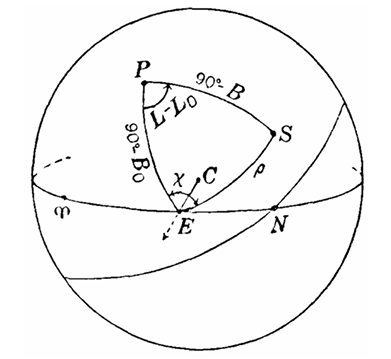
\includegraphics[width=0.44\textwidth]{figures/solar/helio_geom.png}
    \caption{Esquema geométrico de la proyección heliográfica. Se indican la
    latitud heliográfica $B$, la longitud relativa $L-L_0$, la distancia angular
    central $\rho$, el ángulo posicional $\theta$ y la inclinación heliográfica
    $B_0$ del eje solar respecto del observador. \textbf{Fuente:} adaptado de
    \textit{CESAR's Booklet} de la ESA.}
    \label{fig:heliographic-geometry-sw}
\end{figure}

\begin{figure}[H]
    \centering
    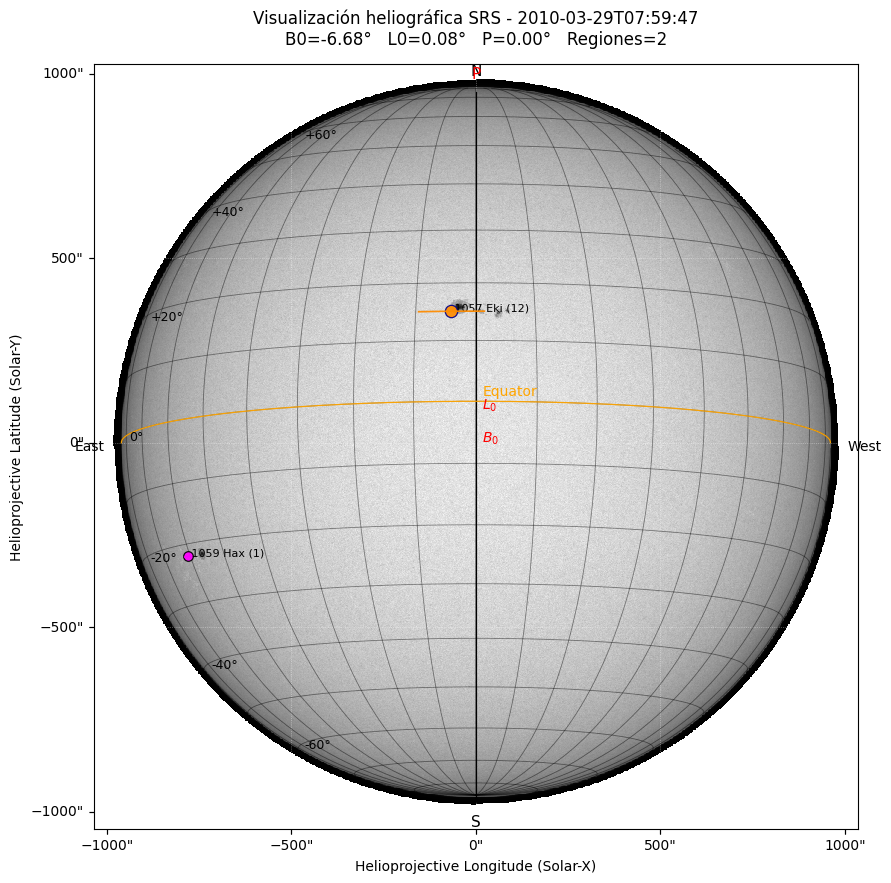
\includegraphics[width=0.8\textwidth]{figures/solar/helio_proj.png}
    \caption{Ejemplo de proyección heliográfica sobre una imagen SDO/HMI con
    retícula solar, ecuador proyectado y regiones activas asociadas al contenido
    NOAA SRD. La visualización permite verificar la coherencia entre posiciones
    heliográficas, latitudes proyectadas y etiquetas morfológicas. \textbf{Fuente:} Elaboración propia.}
    \label{fig:heliographic-projection-sw}
\end{figure}

Siguiendo la formulación geométrica de coordenadas heliográficas, la relación
entre la distancia radial observada $r$, el radio aparente del disco $r_0$ y el
ángulo auxiliar $\psi$ se expresa como
\begin{equation}
\psi = \frac{\alpha}{2}\,\frac{r}{r_0},
\end{equation}
donde $\alpha$ es el diámetro angular aparente del Sol. Bajo la aproximación de
ángulos pequeños, la distancia angular central respecto del centro del disco se
obtiene mediante
\begin{equation}
\rho = \arcsin\!\left(\frac{\psi}{\alpha/2}\right) - \psi.
\end{equation}
Si $(x,y)$ denotan las coordenadas cartesianas de la región activa medidas
respecto del centro del disco, el ángulo posicional se calcula como
\begin{equation}
\theta = \arctan\!\left(\frac{x}{y}\right).
\end{equation}
Conocidos $B_0$, $\rho$ y $\theta$, la latitud heliográfica $B$ queda dada por
\begin{equation}
\sin(B) = \sin(B_0)\cos(\rho) + \cos(B_0)\sin(\rho)\cos(\theta),
\end{equation}
mientras que la longitud heliográfica se recupera a partir de
\begin{equation}
L = \arcsin\!\big(\sin(\rho)\sin(\theta)\cos(B)\big) + L_0,
\end{equation}
donde $L_0$ representa la longitud del meridiano central. Estas ecuaciones
permiten trasladar detecciones en píxeles hacia coordenadas heliográficas antes
de asociarlas con las entradas NOAA SRD \citep{cesarHeliographic,noaaSRS}.

Se generaron dos colecciones diferenciadas. DB1 contiene aproximadamente 4700
imágenes de disco completo de tamaño 1024\,$\times$\,1024 con cajas delimitadoras
asociadas a grupos solares; se utiliza para entrenar el detector. DB2 contiene
alrededor de 15000 recortes derivados de dichas regiones y reinsertados en un
lienzo de 224\,$\times$\,224, preservando proporciones para evitar distorsiones
severas durante el redimensionamiento. DB2 se destina a la clasificación
Zurich--McIntosh.

La construcción de DB2.1 se apoya en una cadena de refinamiento donde el
detector YOLO26n, entrenado sobre DB1, se aplica sobre imágenes preprocesadas
mediante segmentación determinista y realce con filtro \textit{black-hat}. Aunque
el modelo se presenta formalmente en la Sección~\ref{sec:training}, se menciona
en este apartado porque participa en una iteración complementaria sobre los datos
de DB2: sus detecciones permiten ajustar la ubicación de las regiones candidatas,
reconstruir los recortes y obtener una versión DB2.1 con mejor correspondencia
entre imagen, posición y etiqueta. Las regiones candidatas se asocian luego con
el contenido diario de NOAA SRD para recuperar identidad, posición y etiqueta
morfológica, lo que permite generar recortes más consistentes para la
clasificación \citep{sayez2023sunscc,zhou2023mcintosh,noaaSRS}.

\begin{table}[H]
    \centering
    \caption{Resumen de bases de datos utilizadas para entrenamiento y refinamiento. \textbf{Fuente:} Elaboración propia a partir del flujo de construcción de datos.}
    \label{tab:resumen-bases-datos}
    \scriptsize
    \begin{tabular}{lp{0.25\linewidth}cp{0.30\linewidth}}
        \toprule
        \textbf{Base} & \textbf{Unidad} & \textbf{Registros} & \textbf{Uso principal} \\
        \midrule
        DB1 & Disco completo & $\sim$4700 & Entrenamiento de YOLO26n \\
        DB2 & Grupo solar & $\sim$15000 & Etapa intermedia \\
        DB2.1 & Grupo solar refinado (YOLO26n+PCA) & $\sim$14300 & Entrenamiento de ConvNeXtV2a \\
        \bottomrule
    \end{tabular}
\end{table}

Además de distinguir el tipo de imagen, cada base conserva un conjunto mínimo de
metadatos que permite auditar el origen de cada muestra. Esta decisión es
importante porque el entrenamiento no solo requiere imágenes y etiquetas, sino
también la posibilidad de reconstruir la ruta que llevó desde una observación
astronómica hasta un recorte usado por un modelo. La Tabla~\ref{tab:trazabilidad-datos}
resume los campos operativos empleados para mantener esa trazabilidad.

\begin{table}[H]
\centering
\caption{Campos de trazabilidad conservados durante la construcción de datos. \textbf{Fuente:} Elaboración propia.}
\label{tab:trazabilidad-datos}
\scriptsize
\begin{tabular}{p{0.22\textwidth}p{0.31\textwidth}p{0.31\textwidth}}
\toprule
\textbf{Campo} & \textbf{Descripción} & \textbf{Uso dentro del sistema} \\
\midrule
Fecha UTC & Fecha de imagen HMI y reporte NOAA SRD asociado & Unión temporal entre imagen, reporte y predicción \\
Identificador NOAA & Número de región activa reportada & Auditoría de grupo solar y consulta histórica \\
Coordenadas heliográficas & Latitud, longitud y posición relativa en disco & Proyección, recorte y análisis latitudinal \\
Caja delimitadora & Coordenadas normalizadas o absolutas del grupo & Entrenamiento YOLO26n y generación de recortes \\
Etiqueta $ZPC$ & Componentes Zurich, penumbral y compactación & Entrenamiento jerárquico ConvNeXtV2a \\
Ruta/clave de imagen & Referencia a disco completo o recorte & Reproducibilidad, visualización y depuración \\
\bottomrule
\end{tabular}
\end{table}

El diseño de persistencia refleja esa misma separación entre observación,
región activa, recorte e inferencia. En lugar de almacenar únicamente archivos de
imagen, la base se organiza como un repositorio relacional donde una observación
puede contener varias regiones, cada región puede generar uno o más recortes y
cada recorte puede recibir predicciones de modelos distintos. La
Figura~\ref{fig:db-schema-data} muestra la estructura lógica utilizada para
mantener la relación entre datos crudos, metadatos e inferencias.

\begin{figure}[H]
    \centering
    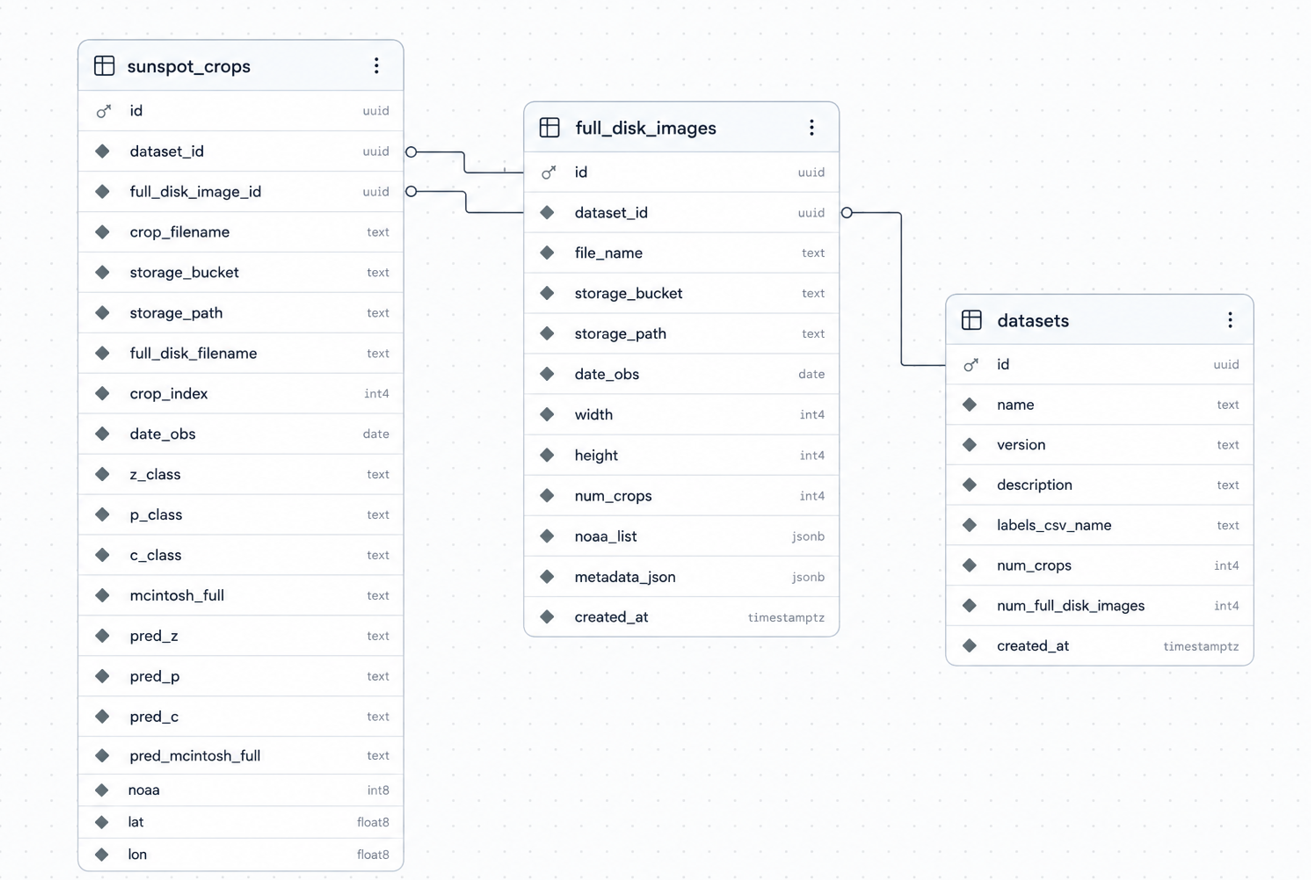
\includegraphics[width=0.92\textwidth]{figures/data/db_schema.png}
    \caption{Esquema lógico de datos para observaciones solares, regiones activas,
    recortes, etiquetas e inferencias. La separación entre entidades permite
    consultar resultados sin perder la relación con la imagen original y los
    metadatos NOAA/SRS. \textbf{Fuente:} Elaboración propia.}
    \label{fig:db-schema-data}
\end{figure}

La construcción de DB2 no consiste simplemente en recortar una vecindad fija
alrededor de cada coordenada NOAA. El procedimiento verifica la posición
proyectada sobre el disco, recorta una región suficientemente amplia para incluir
la estructura completa del grupo y luego reubica el recorte en un lienzo normalizado.
Así se evita deformar grupos alargados o regiones cercanas al limbo, donde la
proyección introduce cambios de escala aparente. La Figura~\ref{fig:hat-db2-pipeline-sw}
resume visualmente esta cadena de construcción.

\begin{figure}[H]
    \centering
    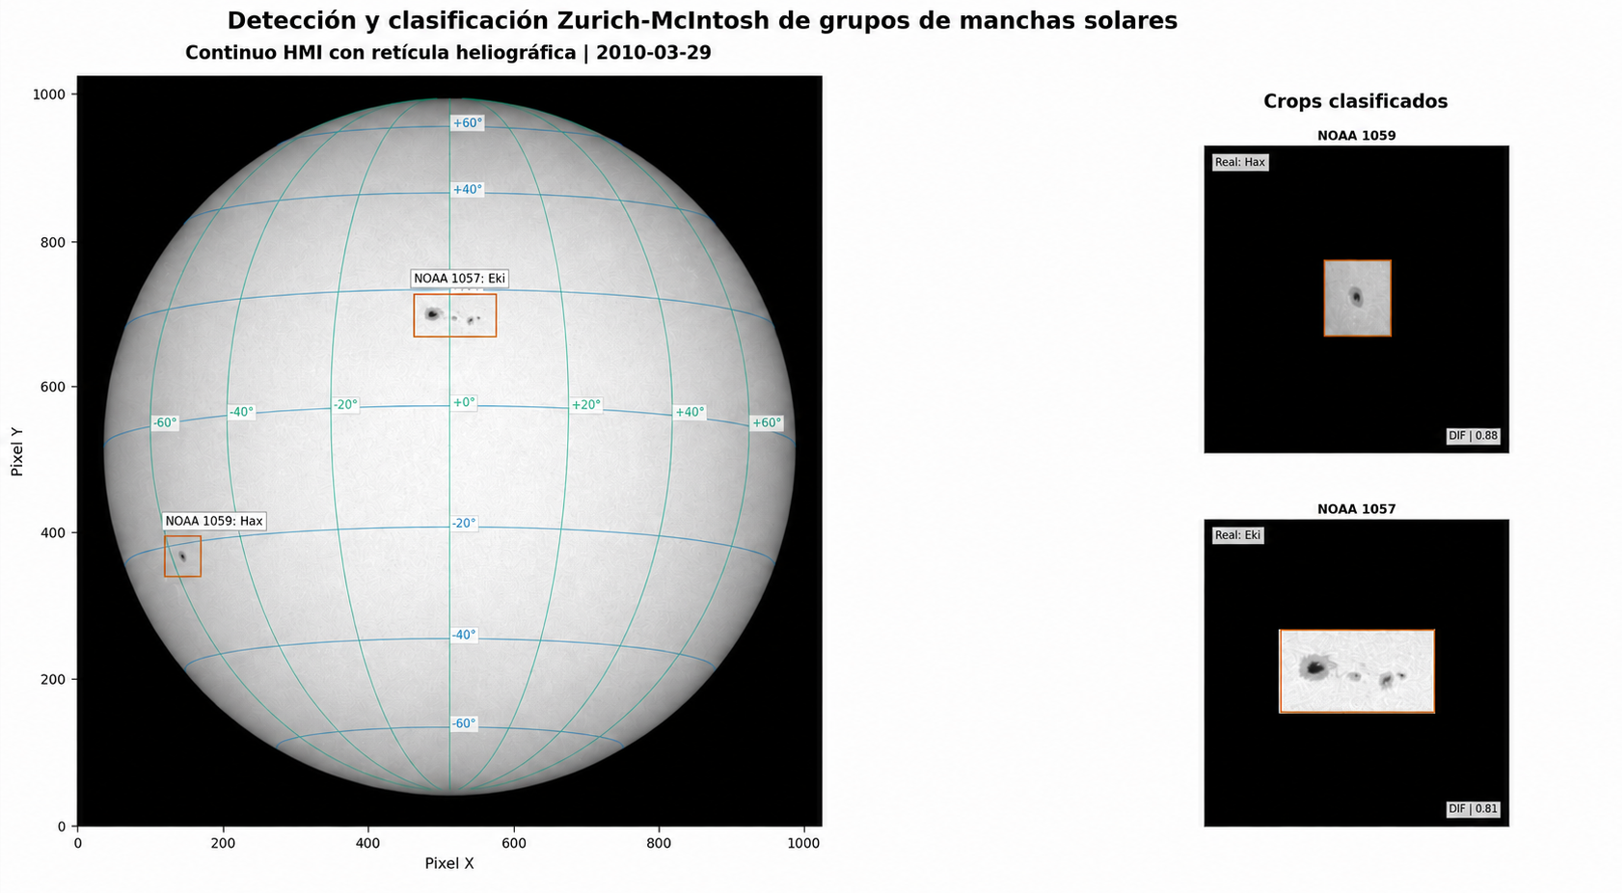
\includegraphics[width=\textwidth]{figures/data/db2_build.png}
    \caption{Construcción ilustrativa de DB2 a partir de una imagen
    SDO/HMI de disco completo con retícula heliográfica. La figura muestra la
    detección de grupos solares sobre el disco, su asociación con regiones NOAA y
    los recortes resultantes utilizados como ejemplos etiquetados para la
    clasificación Zurich--McIntosh. \textbf{Fuente:} Elaboración propia.}
    \label{fig:hat-db2-pipeline-sw}
\end{figure}

La Figura~\ref{fig:db2-zpc-sw} resume la frecuencia de las combinaciones
Zurich--McIntosh presentes en DB2. La distribución es desbalanceada: pocas
configuraciones concentran gran parte de los registros y muchas combinaciones
aparecen con baja frecuencia. Esta estructura condiciona el aprendizaje
supervisado y la interpretación de los errores.

\begin{figure}[H]
    \centering
    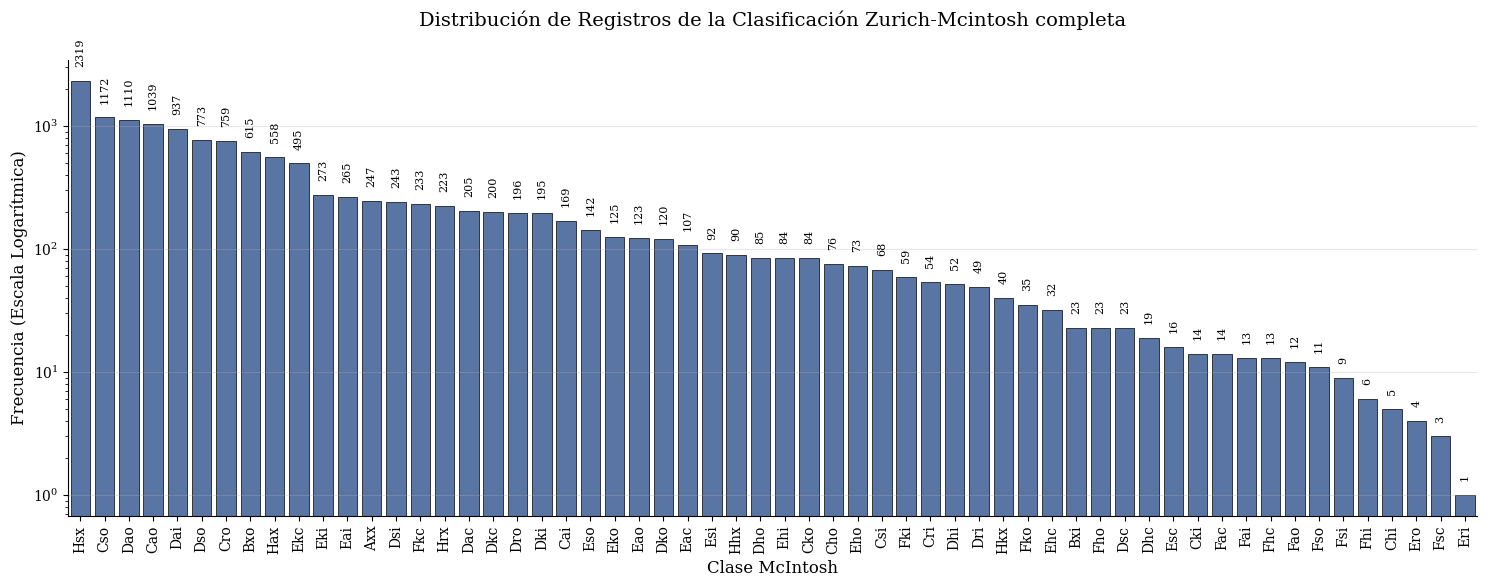
\includegraphics[width=\textwidth]{figures/data/class_hist.png}
    \caption{Histograma de frecuencias por combinación Zurich--McIntosh ($ZPC$)
    de DB2. Se aprecia un régimen de cola larga, donde unas pocas combinaciones
    dominan la muestra total. \textbf{Fuente:} Elaboración propia.}
    \label{fig:db2-zpc-sw}
\end{figure}

La Figura~\ref{fig:db2-caracteres-sw} desagrega la misma base por componente de
la taxonomía. Las distribuciones marginales de $Z$, $P$ y $C$ confirman que el
desbalance no se limita a la combinación completa, sino que afecta cada salida de
forma distinta. Por ello, el entrenamiento requiere ponderación, muestreo
balanceado y evaluación separada por componente.

\begin{figure}[H]
    \centering
    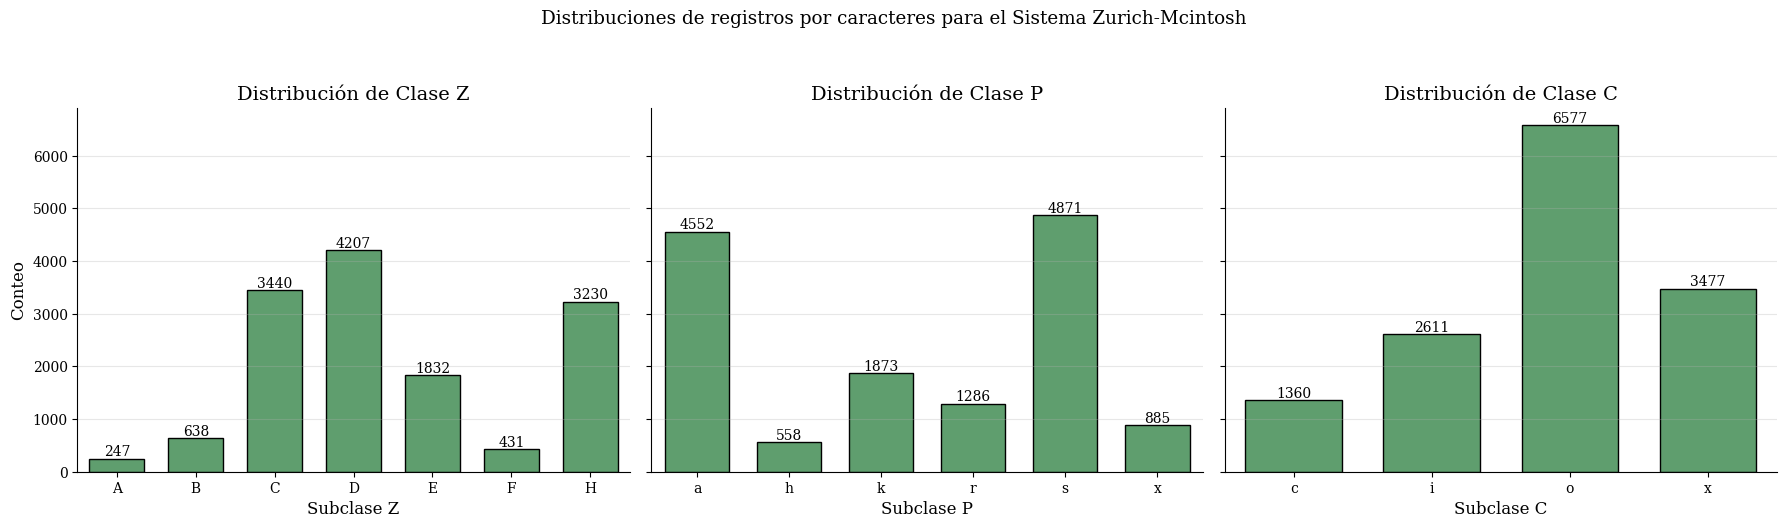
\includegraphics[width=\textwidth]{figures/data/char_hist.png}
    \caption{Histogramas de frecuencias por carácter en DB2 para las componentes
    $Z$, $P$ y $C$ de la clasificación Zurich--McIntosh. La desagregación
    evidencia la asimetría marginal de cada salida. \textbf{Fuente:} Elaboración propia.}
    \label{fig:db2-caracteres-sw}
\end{figure}

Además del desbalance, la generación automática de recortes introduce ruido
residual: regiones parciales, agrupamientos ambiguos o recortes con contaminación
geométrica. Para reducir estos casos se empleó una depuración basada en reducción
de dimensión con PCA y detección de valores atípicos mediante \textit{Isolation
Forest}. Esta etapa no elimina la ambigüedad propia del dominio, pero mejora la
coherencia morfológica del conjunto y favorece un entrenamiento más estable.

Con estas dos bases queda definido el insumo principal de la etapa de aprendizaje
profundo: DB1 permite enseñar al sistema dónde se encuentran los grupos solares
en el disco completo, mientras que DB2 permite enseñar qué morfología presenta
cada región activa una vez recortada. La arquitectura de IA se construye a partir
de esta división funcional.

\section{Entrenamiento de modelos de Deep Learning}
\label{sec:training}

La arquitectura de aprendizaje profundo se organiza como una cascada modular. En
la primera etapa, un detector localiza grupos de manchas solares en imágenes de
disco completo. En la segunda etapa, un clasificador especializado recibe los
recortes generados por el detector y estima las componentes de la taxonomía
Zurich--McIntosh. Esta separación reduce la complejidad de cada tarea: el detector
se concentra en ubicación espacial y el clasificador en morfología local.

El enfoque en cascada también mejora la trazabilidad del sistema. Cada predicción
puede asociarse con una región detectada, una fecha, una posición heliográfica y
una etiqueta taxonómica. En caso de error, es posible distinguir si la falla
proviene de la localización inicial, del recorte utilizado o de la clasificación
morfológica posterior.

\subsection{YOLO26n}

La etapa de agrupamiento se implementa con YOLO26n para localizar grupos de
manchas solares en imágenes de disco completo. El modelo se entrenó sobre DB1, compuesta por imágenes HMI de disco completo con
anotaciones de grupos solares. Antes del entrenamiento definitivo, las etiquetas
obtenidas por acoplamiento entre imágenes y registros observacionales fueron
revisadas en Roboflow, con el fin de corregir cajas desplazadas, regiones
omitidas y detecciones espurias. Esta revisión técnico-visual complementa el etiquetado
automático y mejora la coherencia espacial del conjunto de detección. Además, se
aplicó una aumentación de datos en Roboflow que expandió las 4700 imágenes
etiquetadas originales a 10958 imágenes, utilizando volteo horizontal
(\textit{Flip: Horizontal}) y rotaciones de 90° en sentido horario y antihorario
(\textit{90° Rotate: Clockwise, Counter-Clockwise}). Estas transformaciones
controladas incrementan la robustez frente a cambios de orientación y posición
aparente de las regiones sobre el disco.

\begin{figure}[H]
    \centering
    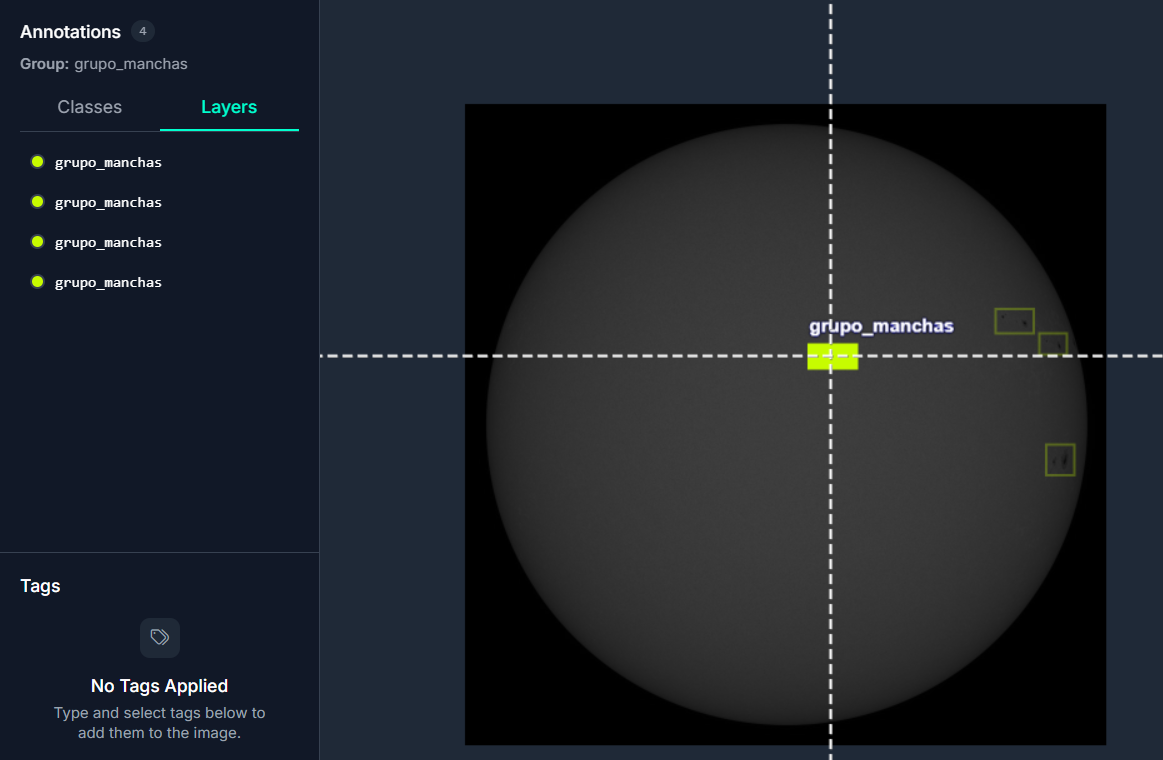
\includegraphics[width=0.92\textwidth]{figures/ml/roboflow.png}
    \caption{Configuración del conjunto de detección en Roboflow, incluyendo la
    revisión de anotaciones y las transformaciones de aumentación aplicadas a las
    imágenes etiquetadas. \textbf{Fuente:} Elaboración propia.}
    \label{fig:roboflow-yolo-augmentation}
\end{figure}

El entrenamiento se realizó durante 200 épocas con tamaño de entrada de 640
píxeles. La configuración final de hiperparámetros se obtuvo mediante Optuna,
explorando tasa de aprendizaje, tamaño de lote, regularización, aumentos de datos
y parámetros de optimización. La selección del modelo consideró métricas estándar
de detección, como precisión, \textit{recall}, intersección sobre unión (IoU) y
precisión media promedio (mAP), junto con la estabilidad de las curvas de pérdida
durante entrenamiento y validación.

Los resultados muestran una convergencia estable y un equilibrio adecuado entre
precisión y exhaustividad para la localización de grupos solares. Sin embargo,
debido a que el entrenamiento se basa en imágenes HMI acopladas con reportes NOAA
SRD, estas métricas deben interpretarse como una validación de la etapa de
localización dentro del dominio fotosférico de entrenamiento. La operación final
en imágenes luz blanca puede requerir ajustes adicionales para compensar
diferencias de contraste, resolución efectiva, \textit{seeing} y condiciones de
adquisición terrestre.

Para el despliegue, el detector se exporta al formato ONNX (\textit{Open Neural
Network Exchange}), en coherencia con la estrategia general de inferencia del
sistema. Esta conversión permite ejecutar el modelo mediante motores compatibles
con entornos locales y web, reduciendo la dependencia del entorno original de
entrenamiento. La portabilidad del detector es especialmente relevante porque la
calidad de sus cajas condiciona las etapas posteriores de recorte, clasificación
y trazabilidad observacional.

La Figura~\ref{fig:yolo-training-results} resume las métricas de entrenamiento
del detector YOLO26n sobre DB1. Las curvas muestran la evolución de las pérdidas
y de los indicadores de precisión, \textit{recall} y mAP, permitiendo verificar
que el modelo alcanza un punto de operación adecuado para construir y refinar
DB2.

\begin{figure}[H]
    \centering
    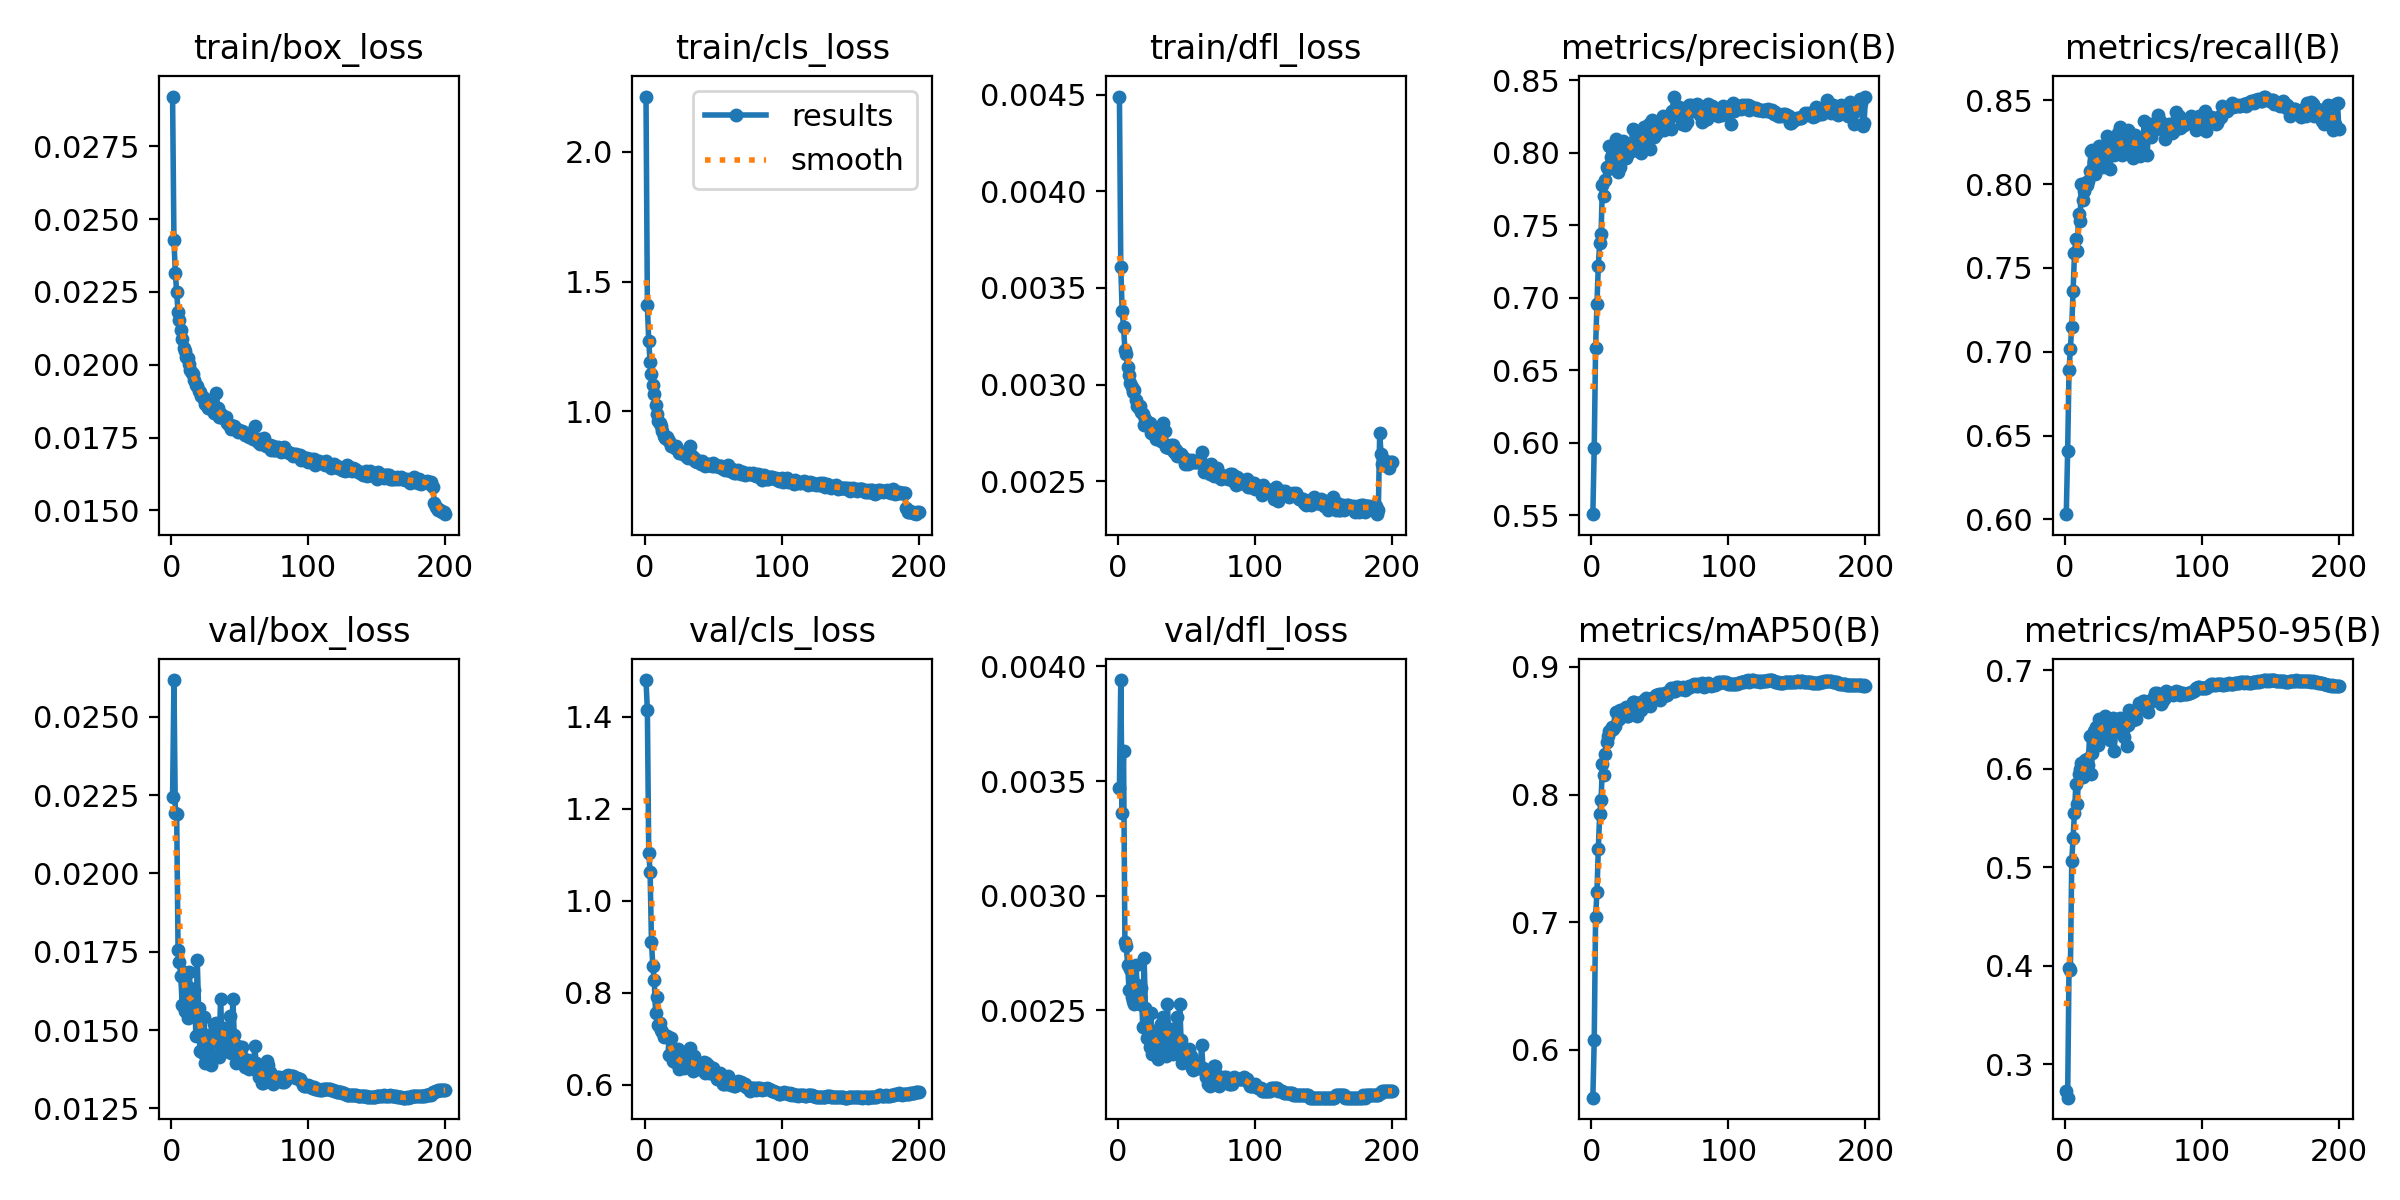
\includegraphics[width=0.92\textwidth]{figures/ml/yolo_results.png}
    \caption{Métricas de entrenamiento del detector YOLO26n sobre DB1. Se
    muestran la evolución de las pérdidas de entrenamiento y validación, junto
    con las métricas de precisión, \textit{recall} y mAP utilizadas para evaluar
    la convergencia del modelo durante el aprendizaje. \textbf{Fuente:} Elaboración propia.}
    \label{fig:yolo-training-results}
\end{figure}

\subsection{ConvNeXtV2}

La etapa de clasificación utiliza ConvNeXtV2 Atto como extractor visual profundo para
inferir las componentes $Z$, $P$ y $C$ de la taxonomía Zurich--McIntosh. El
modelo se inicializa con pesos preentrenados sobre ImageNet y posteriormente se
ajusta finamente sobre la base DB2.1, lo que permite reutilizar representaciones
visuales generales y adaptarlas a rasgos morfológicos característicos de manchas
solares \citep{deng2009imagenet,woo2023convnextv2,zhou2023mcintosh}.

\begin{figure}[H]
    \centering
    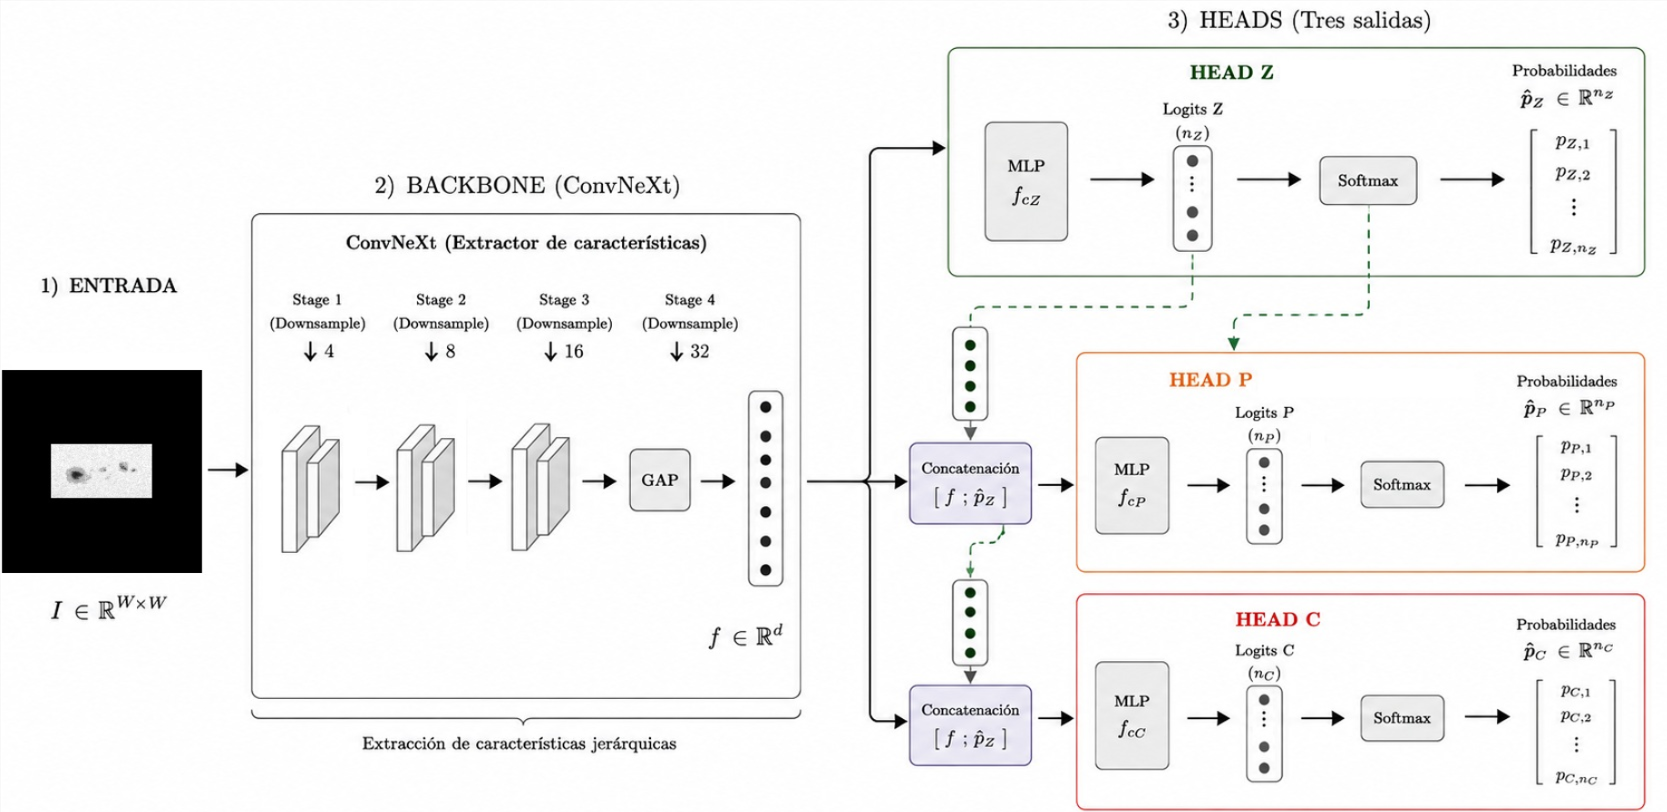
\includegraphics[width=\textwidth]{figures/ml/convnext_arch.png}
    \caption{Arquitectura jerárquica del clasificador ConvNeXtV2 Atto propuesto para
    la inferencia de la taxonomía Zurich--McIntosh. El modelo
    extrae un vector global de características mediante el backbone ConvNeXtV2 y
    genera primero la distribución probabilística del carácter Zurich ($Z$). El
    vector global se obtiene mediante agrupamiento promedio global (GAP), y las
    distribuciones de las componentes $P$ y $C$ se calculan a partir de la
    concatenación $[\mathbf{f};\hat{\mathbf{p}}_Z]$, preservando la estructura
    jerárquica de la taxonomía. \textbf{Fuente:} Elaboración propia.}
    \label{fig:convnextv2-hierarchical}
\end{figure}

La Figura~\ref{fig:convnextv2-hierarchical} resume la arquitectura jerárquica
adoptada. El clasificador recibe recortes de regiones activas insertados en una
matriz de $224 \times 224$ píxeles, preservando la proporción del recorte para
evitar distorsiones por redimensionamiento. Estos recortes provienen de la etapa
YOLO26n y constituyen la entrada del modelo ConvNeXtV2.

El backbone ConvNeXtV2 Atto transforma cada recorte mediante una secuencia de
\textit{stages} jerárquicos con reducciones progresivas de resolución espacial.
Durante el ajuste fino, estos \textit{stages} se incorporan de manera progresiva
al entrenamiento, permitiendo que las capas finales se adapten primero al dominio
solar y que los bloques profundos se actualicen después con menor riesgo de
perder las representaciones generales aprendidas durante el preentrenamiento.
Al final del extractor, una operación de agrupamiento promedio global (GAP,
\textit{Global Average Pooling}) resume los mapas de características en un vector
latente global
\[
\mathbf{f} \in \mathbb{R}^{d},
\]
que concentra información de contraste, textura, geometría y organización del
grupo solar. A partir de esta representación se calcula primero la distribución
del carácter Zurich,
\[
\hat{\mathbf{p}}_Z \in \mathbb{R}^{n_Z},
\]
mediante una salida MLP seguida de Softmax. Las salidas de $P$ y $C$ reciben la
concatenación $[\mathbf{f};\hat{\mathbf{p}}_Z]$, incorporando la dependencia
jerárquica de la taxonomía, y producen
\[
\hat{\mathbf{p}}_P \in \mathbb{R}^{n_P},
\qquad
\hat{\mathbf{p}}_C \in \mathbb{R}^{n_C}.
\]
Por tanto, la salida del modelo se expresa como
\[
f_\theta(x)=
\left(
\hat{\mathbf{p}}_Z,
\hat{\mathbf{p}}_P,
\hat{\mathbf{p}}_C
\right),
\]
donde cada término es una distribución de probabilidad sobre una componente
taxonómica.

Esta descomposición evita tratar cada combinación Zurich--McIntosh como una
clase atómica. Aunque el espacio completo contiene alrededor de 60
configuraciones válidas, el aprendizaje directo sobre combinaciones completas
incrementaría el desbalance y limitaría la generalización en clases raras. La
Figura~\ref{fig:db2-train-val-caracter} muestra que la partición de
entrenamiento y validación conserva la asimetría de DB2 en las tres salidas.

\begin{figure}[H]
    \centering
    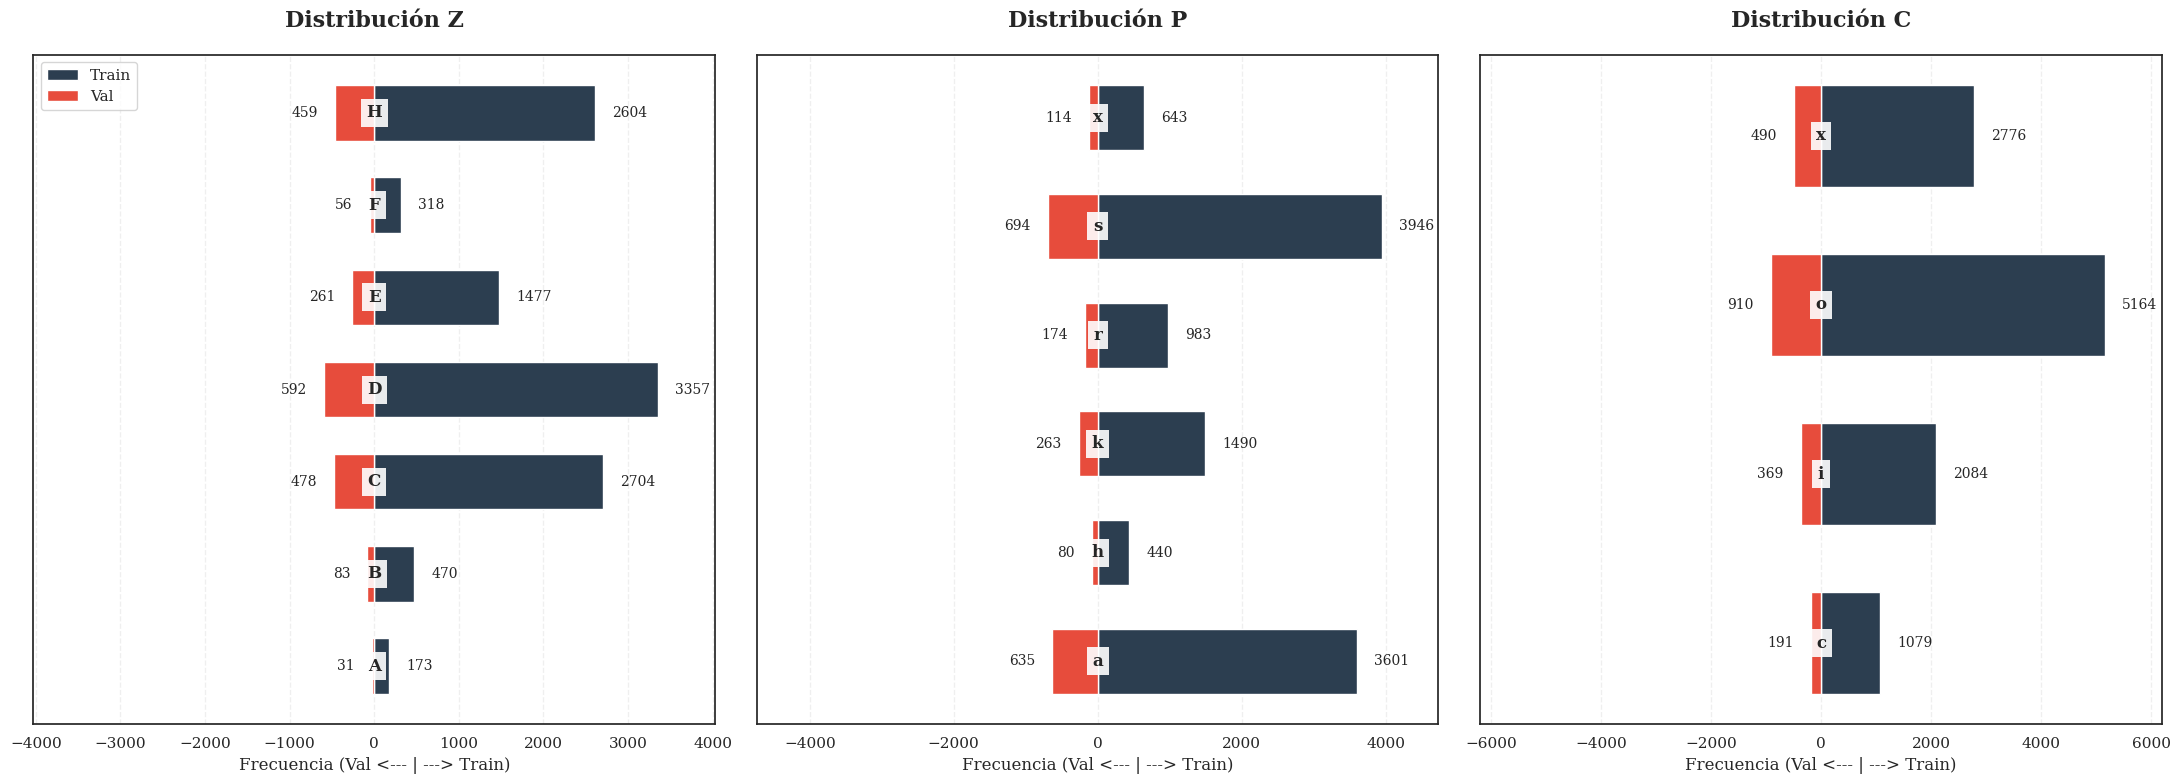
\includegraphics[width=\textwidth]{figures/data/train_val.png}
    \caption{Distribución de frecuencias en los subconjuntos de entrenamiento y
    validación para las componentes $Z$, $P$ y $C$ de la clasificación
    Zurich--McIntosh sobre DB2. La figura muestra que el desbalance de clases se
    mantiene en ambas particiones, con distinta severidad según el carácter
    considerado. \textbf{Fuente:} Elaboración propia.}
    \label{fig:db2-train-val-caracter}
\end{figure}

El entrenamiento mitiga el desbalance mediante pesos basados en el número
efectivo de muestras, muestreo balanceado con \textit{WeightedRandomSampler} y
seguimiento separado de métricas para $Z$, $P$ y $C$ \citep{cui2019classbalanced}.
La arquitectura emplea
Optuna para determinar una configuración óptima de hiperparámetros de
entrenamiento, explorando tasa de aprendizaje, \textit{weight decay}, tamaño de
lote, aumentos, configuración de las salidas MLP y estrategia de ajuste
progresivo de los \textit{stages}. La selección final considera desempeño en
validación, estabilidad de entrenamiento y consistencia entre salidas, no solo la
exactitud global \citep{akiba2019optuna}.

El monitoreo se realiza con curvas de pérdida, exactitud por salida y análisis de
generalización. En los experimentos se observó sobreajuste antes de completar el
máximo de épocas programado, por lo que se conserva el punto con mejor desempeño
en validación. Las Figuras~\ref{fig:cm-z}, \ref{fig:cm-p} y \ref{fig:cm-c}
presentan las matrices de confusión normalizadas: $C$ muestra una separación más
estable, mientras que $Z$ y $P$ concentran ambigüedad en clases fronterizas o con
menor soporte muestral.

Antes de presentar las tablas por clase y las matrices de confusión, se definen
las métricas empleadas para evaluar cada salida del clasificador. Para una clase
$c$ de cualquiera de las salidas $Z$, $P$ o $C$, sean $TP_c$ los verdaderos
positivos, $FP_c$ los falsos positivos y $FN_c$ los falsos negativos. La
precisión de la clase se calcula como
\begin{equation}
\mathrm{Precision}_c=\frac{TP_c}{TP_c+FP_c}.
\end{equation}

El \textit{recall}, o sensibilidad, mide la proporción de ejemplos de la clase
$c$ correctamente recuperados por el modelo:
\begin{equation}
\mathrm{Recall}_c=\frac{TP_c}{TP_c+FN_c}.
\end{equation}

A partir de ambas cantidades, el puntaje F1 se define como la media armónica
entre precisión y \textit{recall}:
\begin{equation}
\mathrm{F1}_c=2\,\frac{\mathrm{Precision}_c\,\mathrm{Recall}_c}{\mathrm{Precision}_c+\mathrm{Recall}_c}.
\end{equation}

En las tablas siguientes se reportan estas métricas por clase y su promedio
ponderado. Este último considera el soporte de cada clase en el conjunto de
validación, por lo que resulta más representativo en presencia de desbalance,
aunque debe interpretarse junto con las métricas individuales para identificar
clases minoritarias o morfológicamente ambiguas.


\begin{table}[H]
\centering
\caption{Resumen de métricas por clase para la salida $Z$. \textbf{Fuente:} Elaboración propia.}
\small
\setlength{\tabcolsep}{8pt}
\renewcommand{\arraystretch}{0.92}
\begin{tabular}{lccc}
\hline
\textbf{Clase} & \textbf{Precisión} & \textbf{Recall} & \textbf{F1} \\ \hline
A & 0.79 & 0.73 & 0.76 \\
B & 0.74 & 0.71 & 0.72 \\
C & 0.68 & 0.61 & 0.64 \\
D & 0.63 & 0.61 & 0.62 \\
E & 0.49 & 0.39 & 0.43 \\
F & 0.47 & 0.39 & 0.43 \\
H & 0.78 & 0.84 & 0.81 \\ \hline
Prom. pond. & 0.68 & 0.63 & 0.65 \\ \hline
\end{tabular}
\end{table}

\begin{figure}[H]
    \centering
    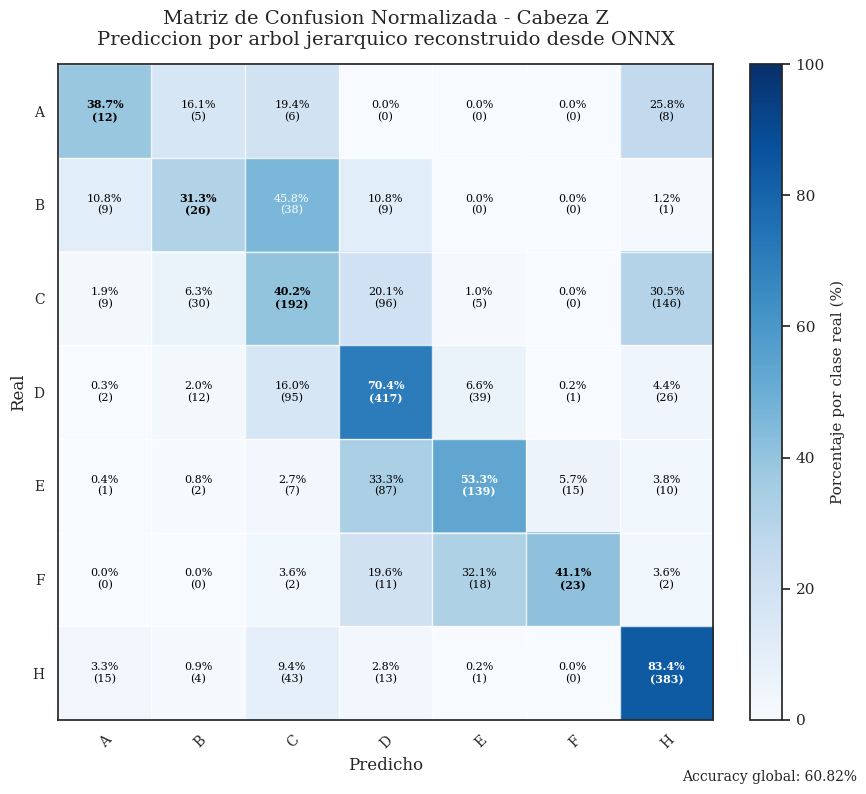
\includegraphics[width=0.75\textwidth]{figures/ml/conf_z.png}
    \caption{Matriz de confusión normalizada para la salida $Z$ del clasificador
    ConvNeXtV2. La diagonal dominante refleja aciertos en varias clases
    principales, mientras que las mayores confusiones se concentran entre
    categorías morfológicamente cercanas. \textbf{Fuente:} Elaboración propia.}
    \label{fig:cm-z}
\end{figure}

\begin{table}[H]
\centering
\caption{Resumen de métricas por clase para la salida $P$. \textbf{Fuente:} Elaboración propia.}
\small
\setlength{\tabcolsep}{8pt}
\renewcommand{\arraystretch}{0.92}
\begin{tabular}{lccc}
\hline
\textbf{Clase} & \textbf{Precisión} & \textbf{Recall} & \textbf{F1} \\ \hline
x & 0.57 & 0.31 & 0.40 \\
r & 0.34 & 0.28 & 0.31 \\
s & 0.59 & 0.63 & 0.61 \\
a & 0.46 & 0.54 & 0.50 \\
h & 0.71 & 0.65 & 0.68 \\
k & 0.84 & 0.82 & 0.83 \\ \hline
Prom. pond. & 0.66 & 0.61 & 0.63 \\ \hline
\end{tabular}
\end{table}

\begin{figure}[H]
    \centering
    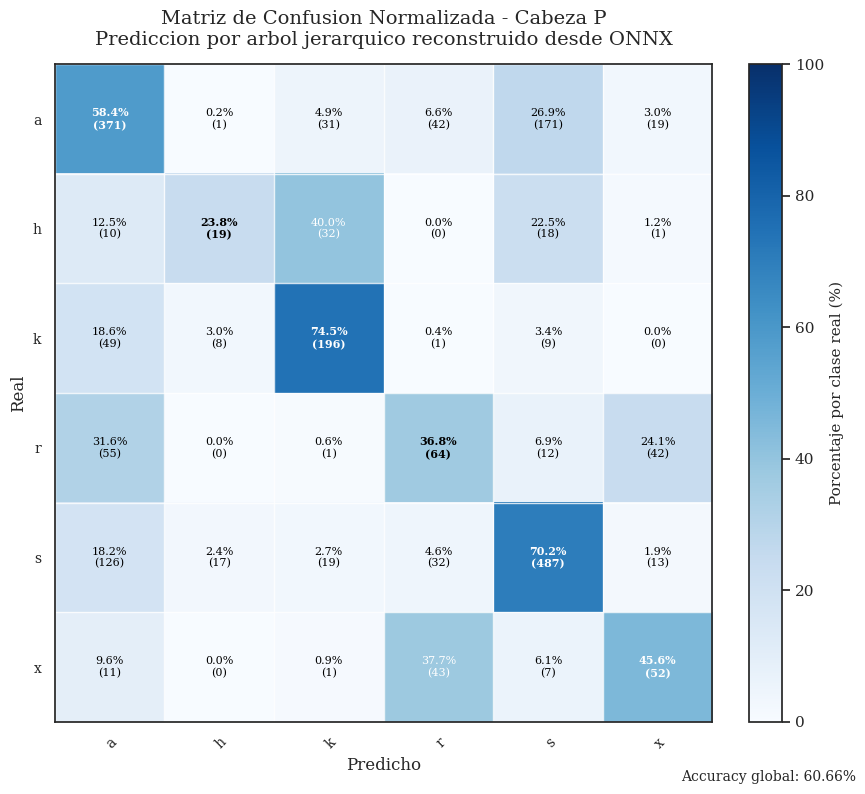
\includegraphics[width=0.75\textwidth]{figures/ml/conf_p.png}
    \caption{Matriz de confusión normalizada para la salida $P$ del modelo
    ConvNeXtV2. Parte importante del error se distribuye entre configuraciones
    penumbrales vecinas, en especial en clases con fuerte desbalance o menor
    número de ejemplos. \textbf{Fuente:} Elaboración propia.}
    \label{fig:cm-p}
\end{figure}

\begin{table}[H]
\centering
\caption{Resumen de métricas por clase para la salida $C$. \textbf{Fuente:} Elaboración propia.}
\small
\setlength{\tabcolsep}{8pt}
\renewcommand{\arraystretch}{0.92}
\begin{tabular}{lccc}
\hline
\textbf{Clase} & \textbf{Precisión} & \textbf{Recall} & \textbf{F1} \\ \hline
x & 0.62 & 0.52 & 0.57 \\
o & 0.46 & 0.47 & 0.46 \\
i & 0.79 & 0.72 & 0.75 \\
c & 0.82 & 0.84 & 0.83 \\ \hline
Prom. pond. & 0.74 & 0.69 & 0.71 \\ \hline
\end{tabular}
\end{table}

\begin{figure}[H]
    \centering
    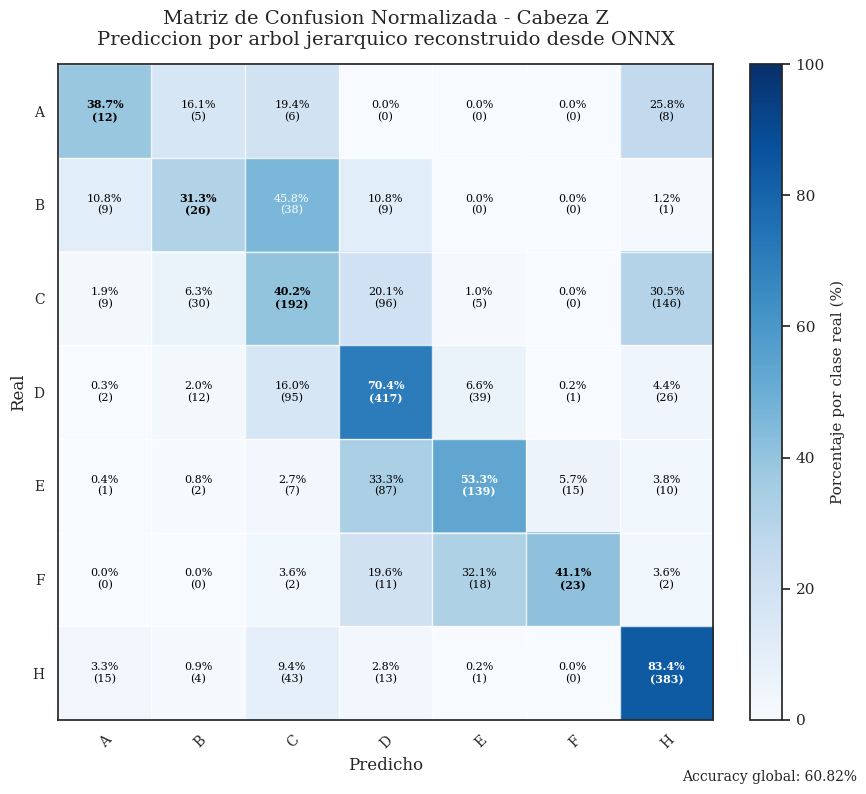
\includegraphics[width=0.75\textwidth]{figures/ml/conf_c.png}
    \caption{Matriz de confusión normalizada para la salida $C$ del clasificador
    ConvNeXtV2. La componente de compactación presenta una estructura de error
    más concentrada sobre la diagonal, lo que sugiere una discriminación
    relativamente más estable que en las otras dos salidas. \textbf{Fuente:} Elaboración propia.}
    \label{fig:cm-c}
\end{figure}

\section{Modelos predictivos}

Los modelos predictivos se presentan como la implementación computacional de la
formulación temporal y espacio-temporal desarrollada en los capítulos anteriores.
A diferencia de detección y clasificación, orientada a interpretar
regiones activas individuales, esta etapa utiliza los datos recopilados en DB1
como base histórica para reconstruir tendencias globales de actividad solar y su
distribución latitudinal, siguiendo la formulación metodológica presentada en la
Sección~\ref{sec:forecast}.

En este contexto, DB1 aporta la secuencia de observaciones de disco completo y
las regiones activas asociadas, permitiendo derivar series temporales del número
de manchas solares y representaciones discretizadas de la actividad por latitud.
Se consideran dos aproximaciones complementarias: un modelo escalar basado en la
trayectoria del número de manchas solares y un modelo espacio-temporal que
reconstruye la distribución latitudinal de la actividad. En ambos casos se evalúa
primero el ajuste de los modelos sobre la dinámica histórica observada y luego se
extiende la predicción hasta el cierre del ciclo solar 25, correspondiente a
finales de 2030. El objetivo no es producir una predicción operacional
definitiva, sino implementar las herramientas formuladas previamente para aportar
contexto temporal y contrastar tendencias con observaciones futuras.

\subsection{Modelo PVL con filtro de Kalman adaptativo}

El modelo PVL con filtro de Kalman adaptativo se utiliza para suavizar y proyectar
la serie temporal del número de manchas solares. La formulación representa la
actividad mediante un estado latente que evoluciona en el tiempo y se actualiza
con observaciones disponibles. La ganancia adaptativa permite ajustar el peso
relativo entre predicción y medición, lo que resulta útil ante ruido observacional
y cambios graduales en la dinámica del ciclo solar
\citep{kalman1960newapproach,podladchikova2012kalman}.

La salida se expresa como $\mathrm{SSN}_{\mathrm{PVLK}}$, una trayectoria escalar
que resume la evolución estimada del índice. Esta aproximación es compacta y
adecuada para describir tendencias globales, aunque no contiene información
espacial sobre la ubicación latitudinal de las regiones activas.

\begin{figure}[H]
    \centering
    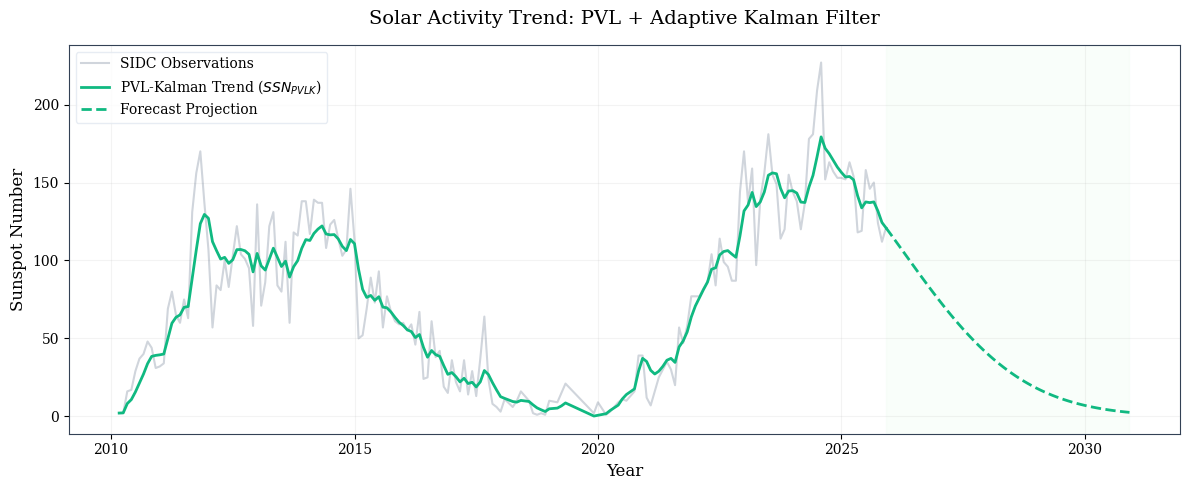
\includegraphics[width=0.92\textwidth]{figures/pred/kalman.png}
    \caption{Ajuste y predicción del número de manchas solares suavizado mediante
    el filtro de Kalman adaptativo ($\mathrm{SSN}_{\mathrm{PVLK}}$). Las líneas
    punteadas corresponden a la predicción. \textbf{Fuente:} Elaboración propia.}
    \label{fig:ssn-kalman-projection}
\end{figure}

\subsection{Modelo espacio-temporal del diagrama de Spörer con DMD}

El segundo enfoque utiliza la Descomposición en Modos Dinámicos (DMD) sobre una
representación latitudinal discretizada de la actividad solar. En lugar de modelar
solo una serie escalar, la actividad se organiza en una malla de latitudes donde
cada celda resume la presencia o intensidad relativa de regiones activas. Esta
representación permite aproximar la evolución espacio-temporal de las bandas de
actividad durante el ciclo solar \citep{schmid2010dmd,kutz2016dmd}.

DMD estima un operador lineal efectivo $\mathbf{A}$ que relaciona estados
consecutivos de la distribución latitudinal. Aunque la dinámica solar real no es
lineal, esta aproximación ofrece una descripción compacta de patrones dominantes
y permite reconstruir la migración progresiva de actividad hacia el ecuador,
rasgo característico del diagrama de Spörer. En términos teóricos, DMD puede
entenderse como una aproximación finita de modos dominantes asociados al operador
de Koopman; por ello puede capturar estructuras lineales efectivas de un sistema
subyacente no lineal cuando la dinámica observada está dominada por patrones
coherentes \citep{kutz2016dmd}.

\subsubsection{Diagrama de mariposa obtenido}

El diagrama de mariposa obtenido resume la evolución latitudinal de la actividad
reconstruida. Esta visualización permite evaluar si el modelo conserva una estructura
físicamente coherente, más allá de su error escalar sobre el número total de
manchas.

\begin{figure}[H]
    \centering
    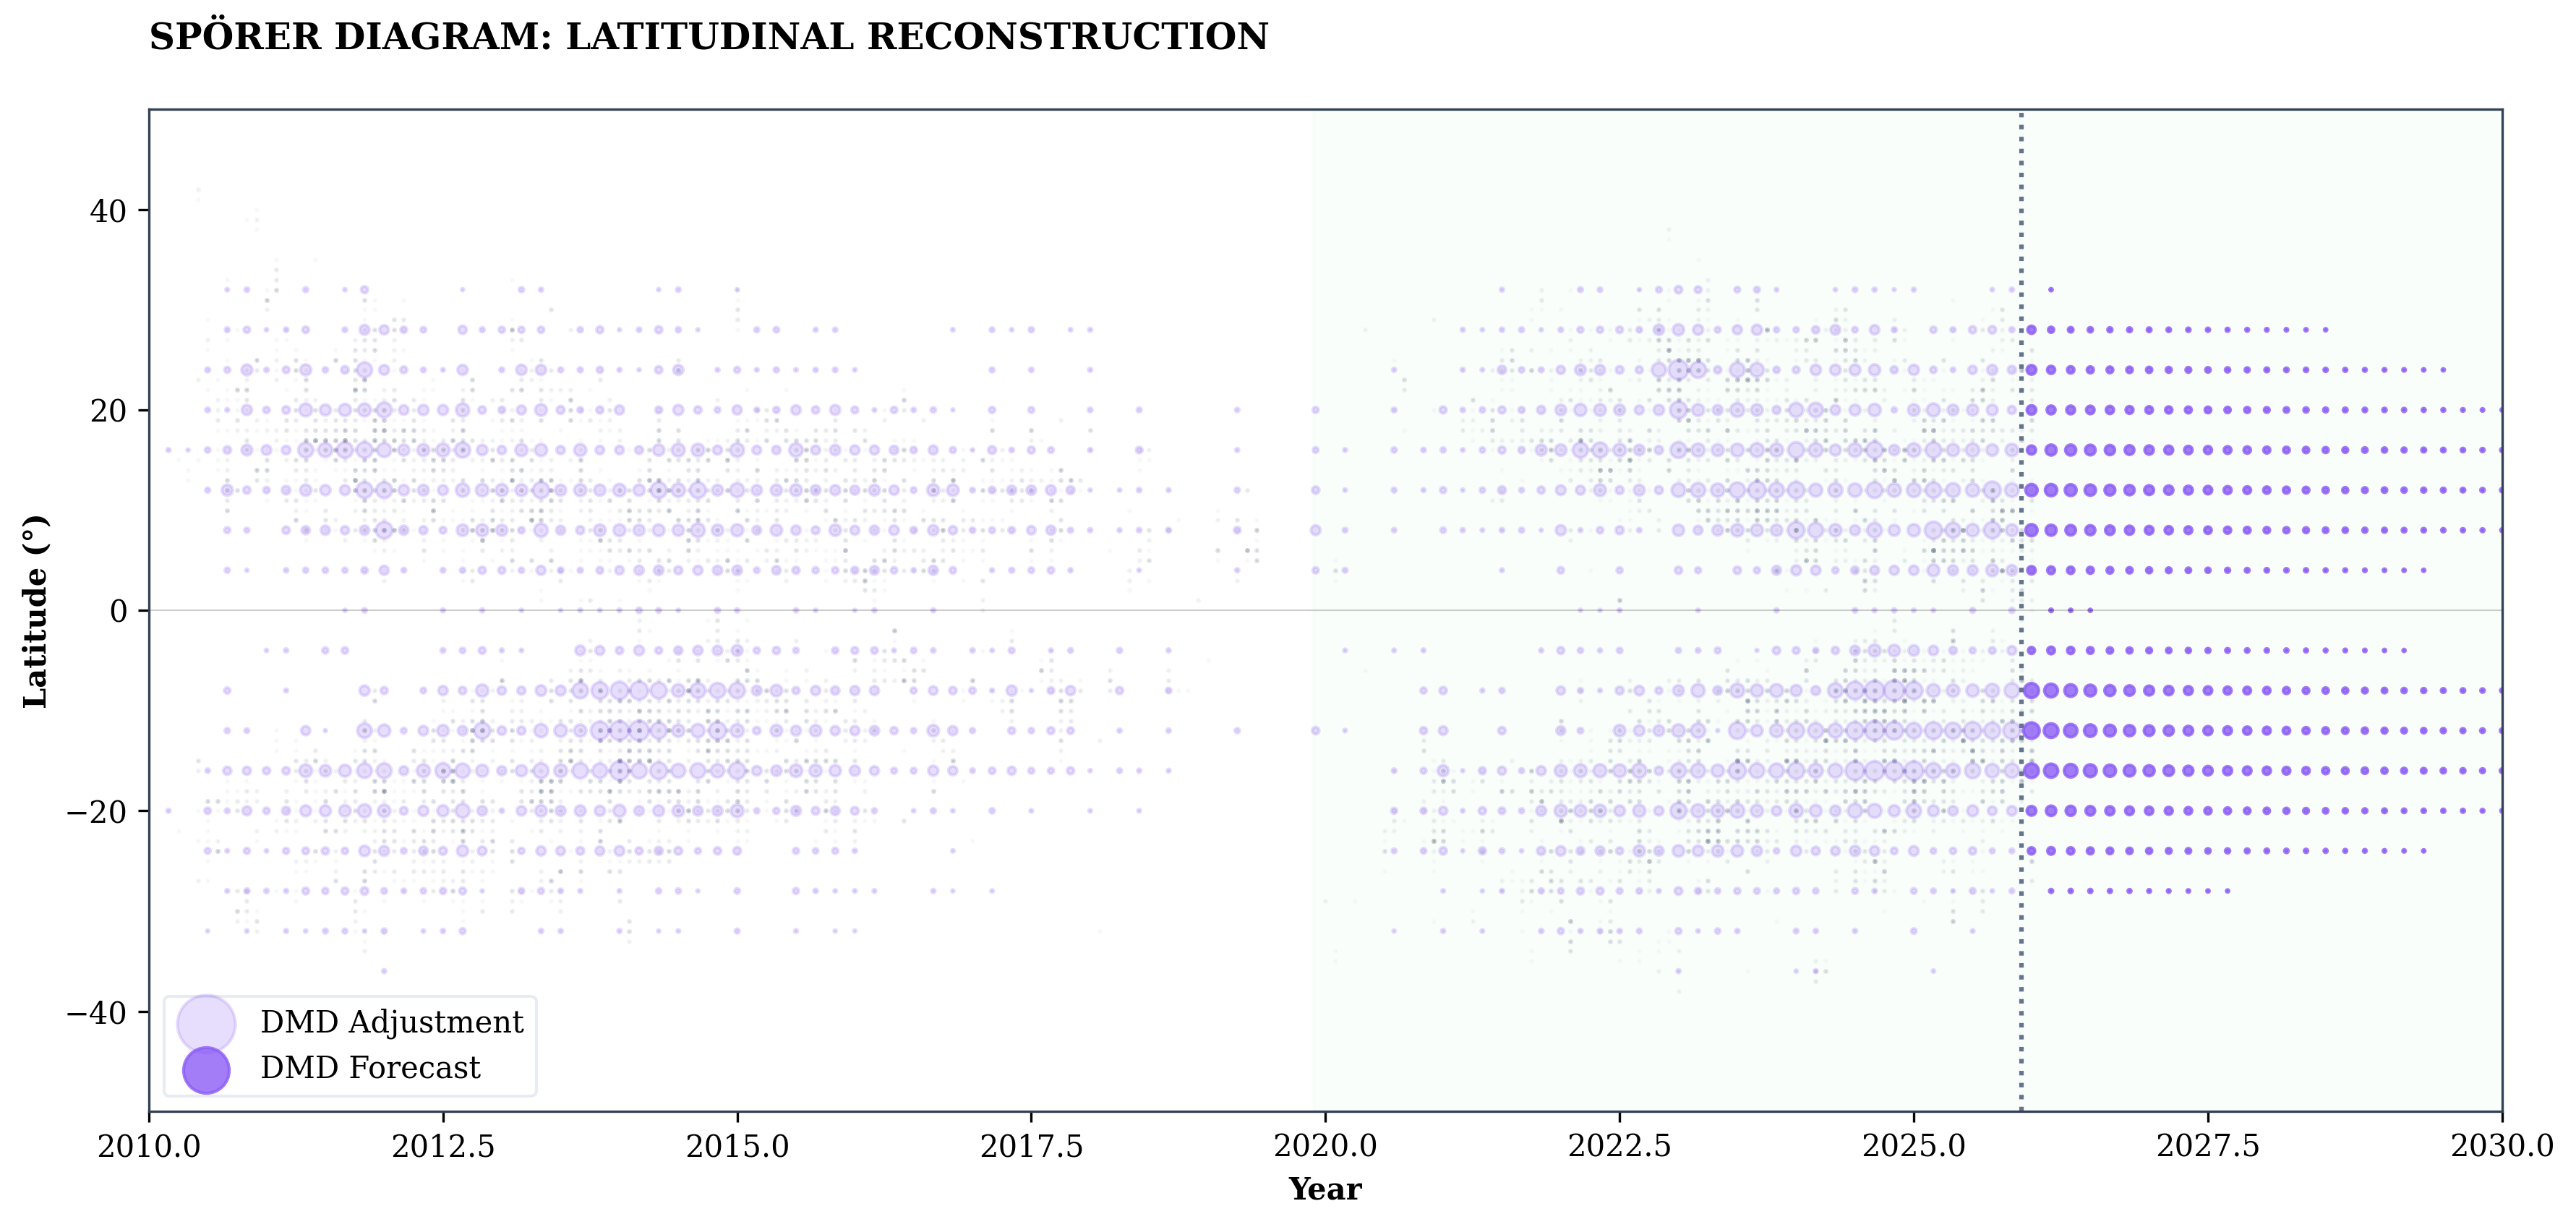
\includegraphics[width=0.92\textwidth]{figures/pred/sporer.png}
    \caption[Ajuste y predicción de la migración latitudinal con DMD]{Ajuste y predicción de la migración latitudinal de la actividad
    solar reconstruida mediante DMD. La figura ilustra el desplazamiento
    progresivo de las bandas activas hacia el ecuador (diagrama de Spörer)
    derivado del operador dinámico $\mathbf{A}$. La región con morado más intenso
    corresponde a la predicción. \textbf{Fuente:} Elaboración propia.}
    \label{fig:sporer-migration-model}
\end{figure}

\subsubsection{Cálculo del SSN por integral discreta}

Para comparar el modelo DMD con una serie escalar, la distribución latitudinal
reconstruida se reduce mediante una integral discreta sobre las celdas de la
malla. Manteniendo la misma formulación de la Sección~\ref{sec:forecast}, si
$\widehat{V}_j(t)$ representa la actividad estimada en la celda latitudinal $j$
para el instante $t$, el índice reconstruido se expresa como
\begin{equation}
\mathrm{SSN}_{\mathrm{DMD}}(t)=\kappa\sum_{j=1}^{M}\widehat{V}_j(t),
\end{equation}
donde $\kappa$ calibra la suma latitudinal respecto a la escala histórica:
\begin{equation}
\kappa=\frac{\sum_{t=1}^{N}\mathrm{SSN}_{\mathrm{obs}}(t)}{\sum_{t=1}^{N}\sum_{j=1}^{M}\widehat{V}_j(t)}.
\end{equation}
Esta operación no reemplaza la interpretación espacial del modelo; solo permite
obtener una magnitud comparable con el número de manchas solares tradicional.

\begin{figure}[H]
    \centering
    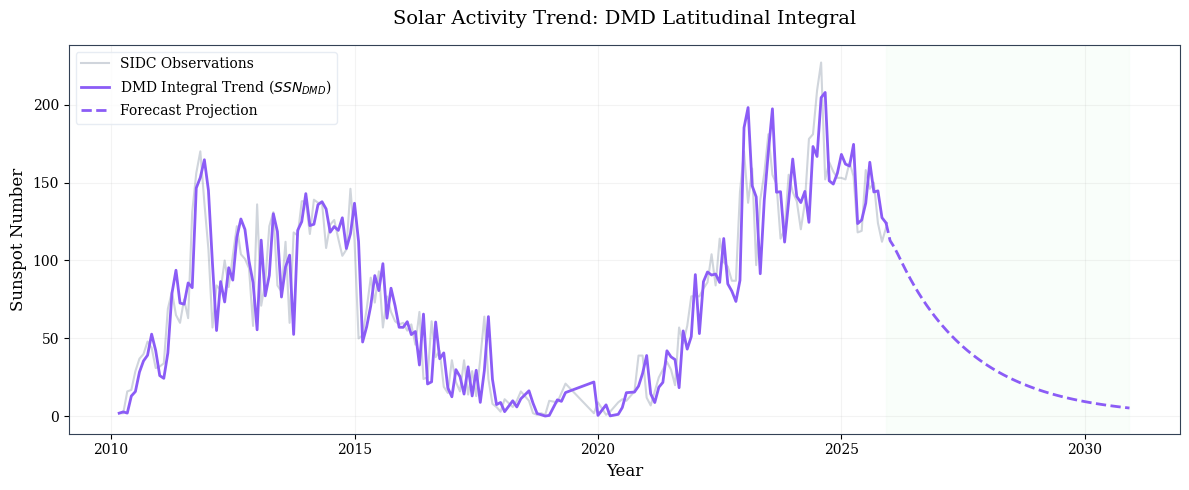
\includegraphics[width=0.92\textwidth]{figures/pred/dmd.png}
    \caption{Ajuste y predicción del número de manchas solares derivada de la
    integral latitudinal del modelo DMD ($\mathrm{SSN}_{\mathrm{DMD}}$). Las
    líneas punteadas corresponden a la predicción. \textbf{Fuente:} Elaboración
    propia.}
    \label{fig:ssn-dmd-projection}
\end{figure}


\section{Arquitectura y despliegue de base de datos}

La persistencia de datos se organiza mediante una base relacional desplegada en
Supabase sobre PostgreSQL. Esta capa conserva tanto los datos derivados de la
etapa de entrenamiento como los nuevos registros capturados desde la Raspberry Pi
5. La base no se limita a almacenar imágenes; mantiene la relación entre
conjuntos de datos, discos solares completos, recortes de manchas, predicciones,
metadatos de observación y capturas operativas recientes.

La base de datos actúa como punto de unión entre las etapas anteriores y la
plataforma web. En ella confluyen las imágenes de origen, las etiquetas usadas
para entrenamiento, las inferencias del detector y del clasificador, y los
productos de observación generados durante la operación del prototipo. Esta
centralización evita que la trazabilidad dependa de archivos aislados y permite
reconstruir el historial completo de cada observación.

\begin{figure}[H]
    \centering
    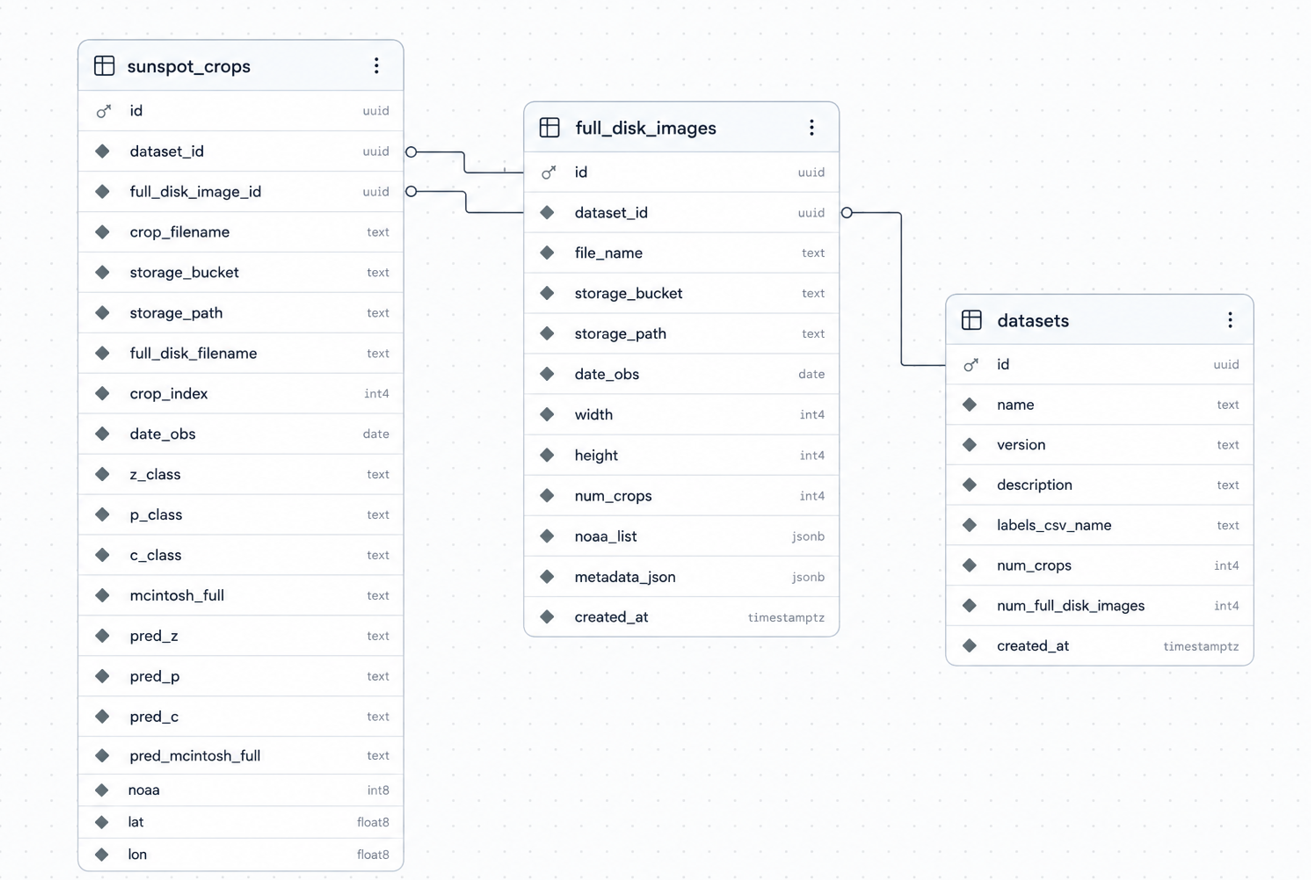
\includegraphics[width=0.95\textwidth]{figures/data/db_schema.png}
    \caption{Estructura relacional de la base de datos desplegada en Supabase.
    El esquema vincula conjuntos de datos, imágenes de disco completo, recortes
    de manchas solares y capturas recientes generadas desde la Raspberry Pi 5. \textbf{Fuente:} Elaboración propia.}
    \label{fig:db-structure-supabase}
\end{figure}


La arquitectura se apoya en tres tablas principales para los conjuntos
históricos. La tabla \texttt{datasets} identifica cada colección mediante un
\texttt{id} de tipo UUID, nombre, versión, descripción, archivo de etiquetas y
conteos generales de recortes e imágenes de disco completo. Esta entidad permite
separar versiones de datos, mantener trazabilidad sobre la procedencia de los
registros y evitar ambigüedades cuando se incorporan nuevos conjuntos.

La tabla \texttt{full\_disk\_images} almacena las imágenes de disco completo
asociadas a un \texttt{dataset}. Para cada imagen se registra el nombre del
archivo, el \textit{bucket} de almacenamiento, la ruta del objeto, la fecha de
observación, dimensiones, número de recortes asociados, lista NOAA y metadatos en
formato \texttt{jsonb}. Esta tabla funciona como punto de enlace entre la imagen
solar completa y las regiones activas extraídas a partir de ella.

Los recortes individuales se almacenan en \texttt{sunspot\_crops}. Esta tabla
contiene la referencia al conjunto de datos y a la imagen de disco completo, el
nombre y ruta del recorte, el índice de recorte, la fecha de observación, las
etiquetas reales $Z$, $P$, $C$, la combinación McIntosh completa, las predicciones
del modelo, la identificación NOAA, coordenadas heliográficas, longitud de
Carrington, extensión, área, clase magnética, número de manchas reportado por
SRD, tamaño original del recorte, confianza YOLO y centro de la detección en
píxeles. Con ello, cada recorte conserva simultáneamente información visual,
taxonómica, geométrica y operacional.

El esquema incorpora restricciones de unicidad para preservar consistencia. Por
ejemplo, \texttt{datasets} evita repetir una misma combinación de nombre y
versión; \texttt{full\_disk\_images} impide duplicar archivos dentro de un mismo
conjunto y rutas de almacenamiento; \texttt{sunspot\_crops} evita repetir nombres
de recortes por conjunto, rutas de objetos y pares \texttt{full\_disk\_image\_id}
-- \texttt{crop\_index}. Además, las claves foráneas utilizan eliminación en
cascada, por lo que al retirar un conjunto de datos también se eliminan sus
imágenes y recortes asociados, manteniendo integridad referencial.

Para facilitar consultas frecuentes se definen índices sobre identificadores de
conjunto, fecha de observación, imagen de disco completo, número NOAA y
clasificación McIntosh completa. Estos índices son relevantes para operaciones
como recuperar todos los recortes de una fecha, buscar regiones asociadas a una
NOAA específica, filtrar por combinación Zurich--McIntosh o reconstruir el
historial de una imagen de disco completo.

Las claves foráneas, restricciones de unicidad e índices sobre fecha,
identificador de conjunto, imagen de disco completo, NOAA y clasificación
McIntosh permiten reconstruir la trazabilidad de cada observación y acelerar
consultas frecuentes. Los archivos se conservan en Supabase Storage, incluyendo
el \textit{bucket} privado \texttt{snapshots}, mientras que PostgreSQL almacena
las rutas y metadatos necesarios para su recuperación. La tabla
\texttt{live\_captures} utiliza seguridad a nivel de fila, lo que permite
controlar el acceso desde la plataforma web sin perder la capacidad de consulta y
sincronización.

\section{Plataforma web}

La plataforma web constituye la capa de interacción del sistema. Su función es
convertir los datos persistidos y los modelos desplegados en herramientas de
consulta, visualización e inferencia accesibles para el usuario. Así, el flujo
iniciado con la construcción de datos y el entrenamiento de modelos culmina en
una interfaz capaz de mostrar observaciones, resultados taxonómicos, capturas
recientes y productos predictivos.

\subsection{Desarrollo en Next.js con despliegue en Vercel}

La plataforma web se implementa con Next.js y se despliega en
Vercel como interfaz centralizada para gestión, consulta y análisis de
observaciones solares. Este entorno complementa el procesamiento en el borde
realizado por la Raspberry Pi 5, aportando trazabilidad histórica, visualización
de resultados y acceso remoto. La persistencia y seguridad se apoyan en
Supabase, que gestiona autenticación, metadatos y almacenamiento de
productos derivados.

La arquitectura mantiene separación de responsabilidades en los siguientes
niveles:
\begin{itemize}
    \item Capa de interfaz: Componentes reactivos diseñados para la visualización dinámica de imágenes de disco solar y resultados de inferencia.
    \item Capa de datos y servicios: Módulos de comunicación con la base de datos PostgreSQL para consultas históricas y generación de informes de observación.
    \item Módulos de inferencia: Implementación de motores de ejecución para modelos ONNX directamente en el lado del cliente (navegador).
    \item Visualización predictiva: Herramientas gráficas para el análisis de la distribución latitudinal de manchas (diagramas de mariposa) y la evolución temporal del número de manchas solares (SSN).
\end{itemize}

El sistema opera bajo un esquema híbrido: la adquisición y el preprocesamiento se
ejecutan en el nodo de observación, mientras que la plataforma web mantiene la
disponibilidad remota, la consulta histórica y el soporte a la interpretación
científica.

\label{sec:web}


\subsection{Conversión y despliegue de modelos de procesamiento de imagen a ONNX para inferencia local en el dispositivo}

Los modelos de detección y clasificación se convierten al formato ONNX
(\textit{Open Neural Network Exchange}) para desacoplar la inferencia del entorno
de entrenamiento. Una vez exportados, pueden ejecutarse sin depender de PyTorch,
preservando la estructura computacional y los parámetros aprendidos. Esta
interoperabilidad facilita el despliegue en servidores ligeros, aplicaciones de
escritorio, dispositivos embebidos y navegadores web mediante ONNX
Runtime Web.

En el caso del detector YOLO26n, la entrada del modelo corresponde a una imagen
de disco solar completo previamente normalizada y redimensionada al tamaño
requerido por la red. Para el clasificador jerárquico basado en ConvNeXtV2 Atto, la
entrada consiste en recortes individuales de regiones activas ajustados a
$224 \times 224$ píxeles. La variante Atto se emplea para favorecer una
exportación íntegra desde PyTorch hacia ONNX, mientras que los salidales MLP
conservan el aprendizaje jerárquico de $Z$, $P$ y $C$. En ambos casos, la
exportación conserva la forma del tensor de entrada, el orden de canales, los
factores de normalización y la estructura exacta de las salidas.

Cada modelo exportado se valida comparando sus predicciones con las del entorno
original. Esta verificación confirma la consistencia numérica de la conversión y
permite detectar incompatibilidades de preprocesamiento, dimensiones, orden de
canales o lectura de salidas.

El despliegue \textit{on-device} consiste en ejecutar la inferencia directamente
en el dispositivo del usuario o en el nodo local de observación, evitando que
cada imagen deba enviarse a un servidor remoto para su procesamiento. En la
plataforma desarrollada, esta estrategia permite que los modelos ONNX se
ejecuten dentro del navegador web mediante la biblioteca ONNX Runtime Web. 
Este motor de inferencia utiliza WebAssembly (WASM) para la ejecución 
eficiente en CPU y la API de WebGPU (o WebGL como alternativa) para la 
aceleración por hardware, permitiendo realizar la inferencia localmente con 
un rendimiento cercano al nativo.

Operativamente, esta decisión reduce latencia, ancho de banda y dependencia de
servicios externos de inferencia. Aunque el procesamiento se ejecuta localmente,
los resultados se almacenan junto con imágenes y metadatos observacionales,
manteniendo trazabilidad y permitiendo consulta, revisión y comparación posterior
desde la plataforma web.
\chapter[Resultados y validación]{Resultados y validación\label{cap:resultados}}

\section{Resultados experimentales}
\label{sec:results}

Este capítulo presenta los resultados obtenidos para los tres componentes
analíticos principales del prototipo: el agrupamiento automático de manchas
solares, la clasificación jerárquica Zurich--McIntosh y los modelos predictivos
de actividad solar. Más allá de la evaluación aislada de cada algoritmo, el
objetivo es analizar el comportamiento del sistema como una arquitectura
integrada orientada al registro y procesamiento asistido de observaciones
heliográficas. Esta organización es coherente con la estructura general del
trabajo descrita en el Capítulo 5 y con la validación integral del prototipo
presentada posteriormente. 

\subsection{Agrupamiento automático con YOLO26n}

En la etapa de agrupamiento, el detector basado en YOLO26n alcanzó una
precisión del orden del $83\%$ sobre el conjunto DB1, valor consistente con el
rango de desempeño reportado en la literatura para tareas equivalentes de
detección y agrupamiento de manchas solares en imágenes de disco completo.
Este resultado sugiere que el modelo logra identificar de forma robusta las
regiones activas relevantes y proporciona recortes suficientemente consistentes
para la etapa posterior de clasificación morfológica.

Debe señalarse que la evaluación de esta etapa no persigue una segmentación
pixel a pixel de umbra y penumbra, sino la delimitación espacial de regiones
activas como unidad observacional. Desde esta perspectiva, el rendimiento
obtenido se considera adecuado para el propósito del prototipo, ya que la
clasificación Zurich--McIntosh se aplica sobre grupos solares y no sobre manchas
aisladas.

\subsection{Clasificación jerárquica Zurich--McIntosh}

Antes de la comparación cuantitativa con trabajos de referencia, se analiza el
comportamiento probabilístico de la salida jerárquica propuesta. La
Figura~\ref{fig:resultados-arbol-top12-zpc} muestra el árbol bayesiano de
probabilidades para un caso representativo, donde la recomendación de clase no se
obtiene únicamente como una salida plana, sino como una combinación restringida
por la estructura válida de la taxonomía Zurich--McIntosh. 

\begin{figure}[H]
    \centering
    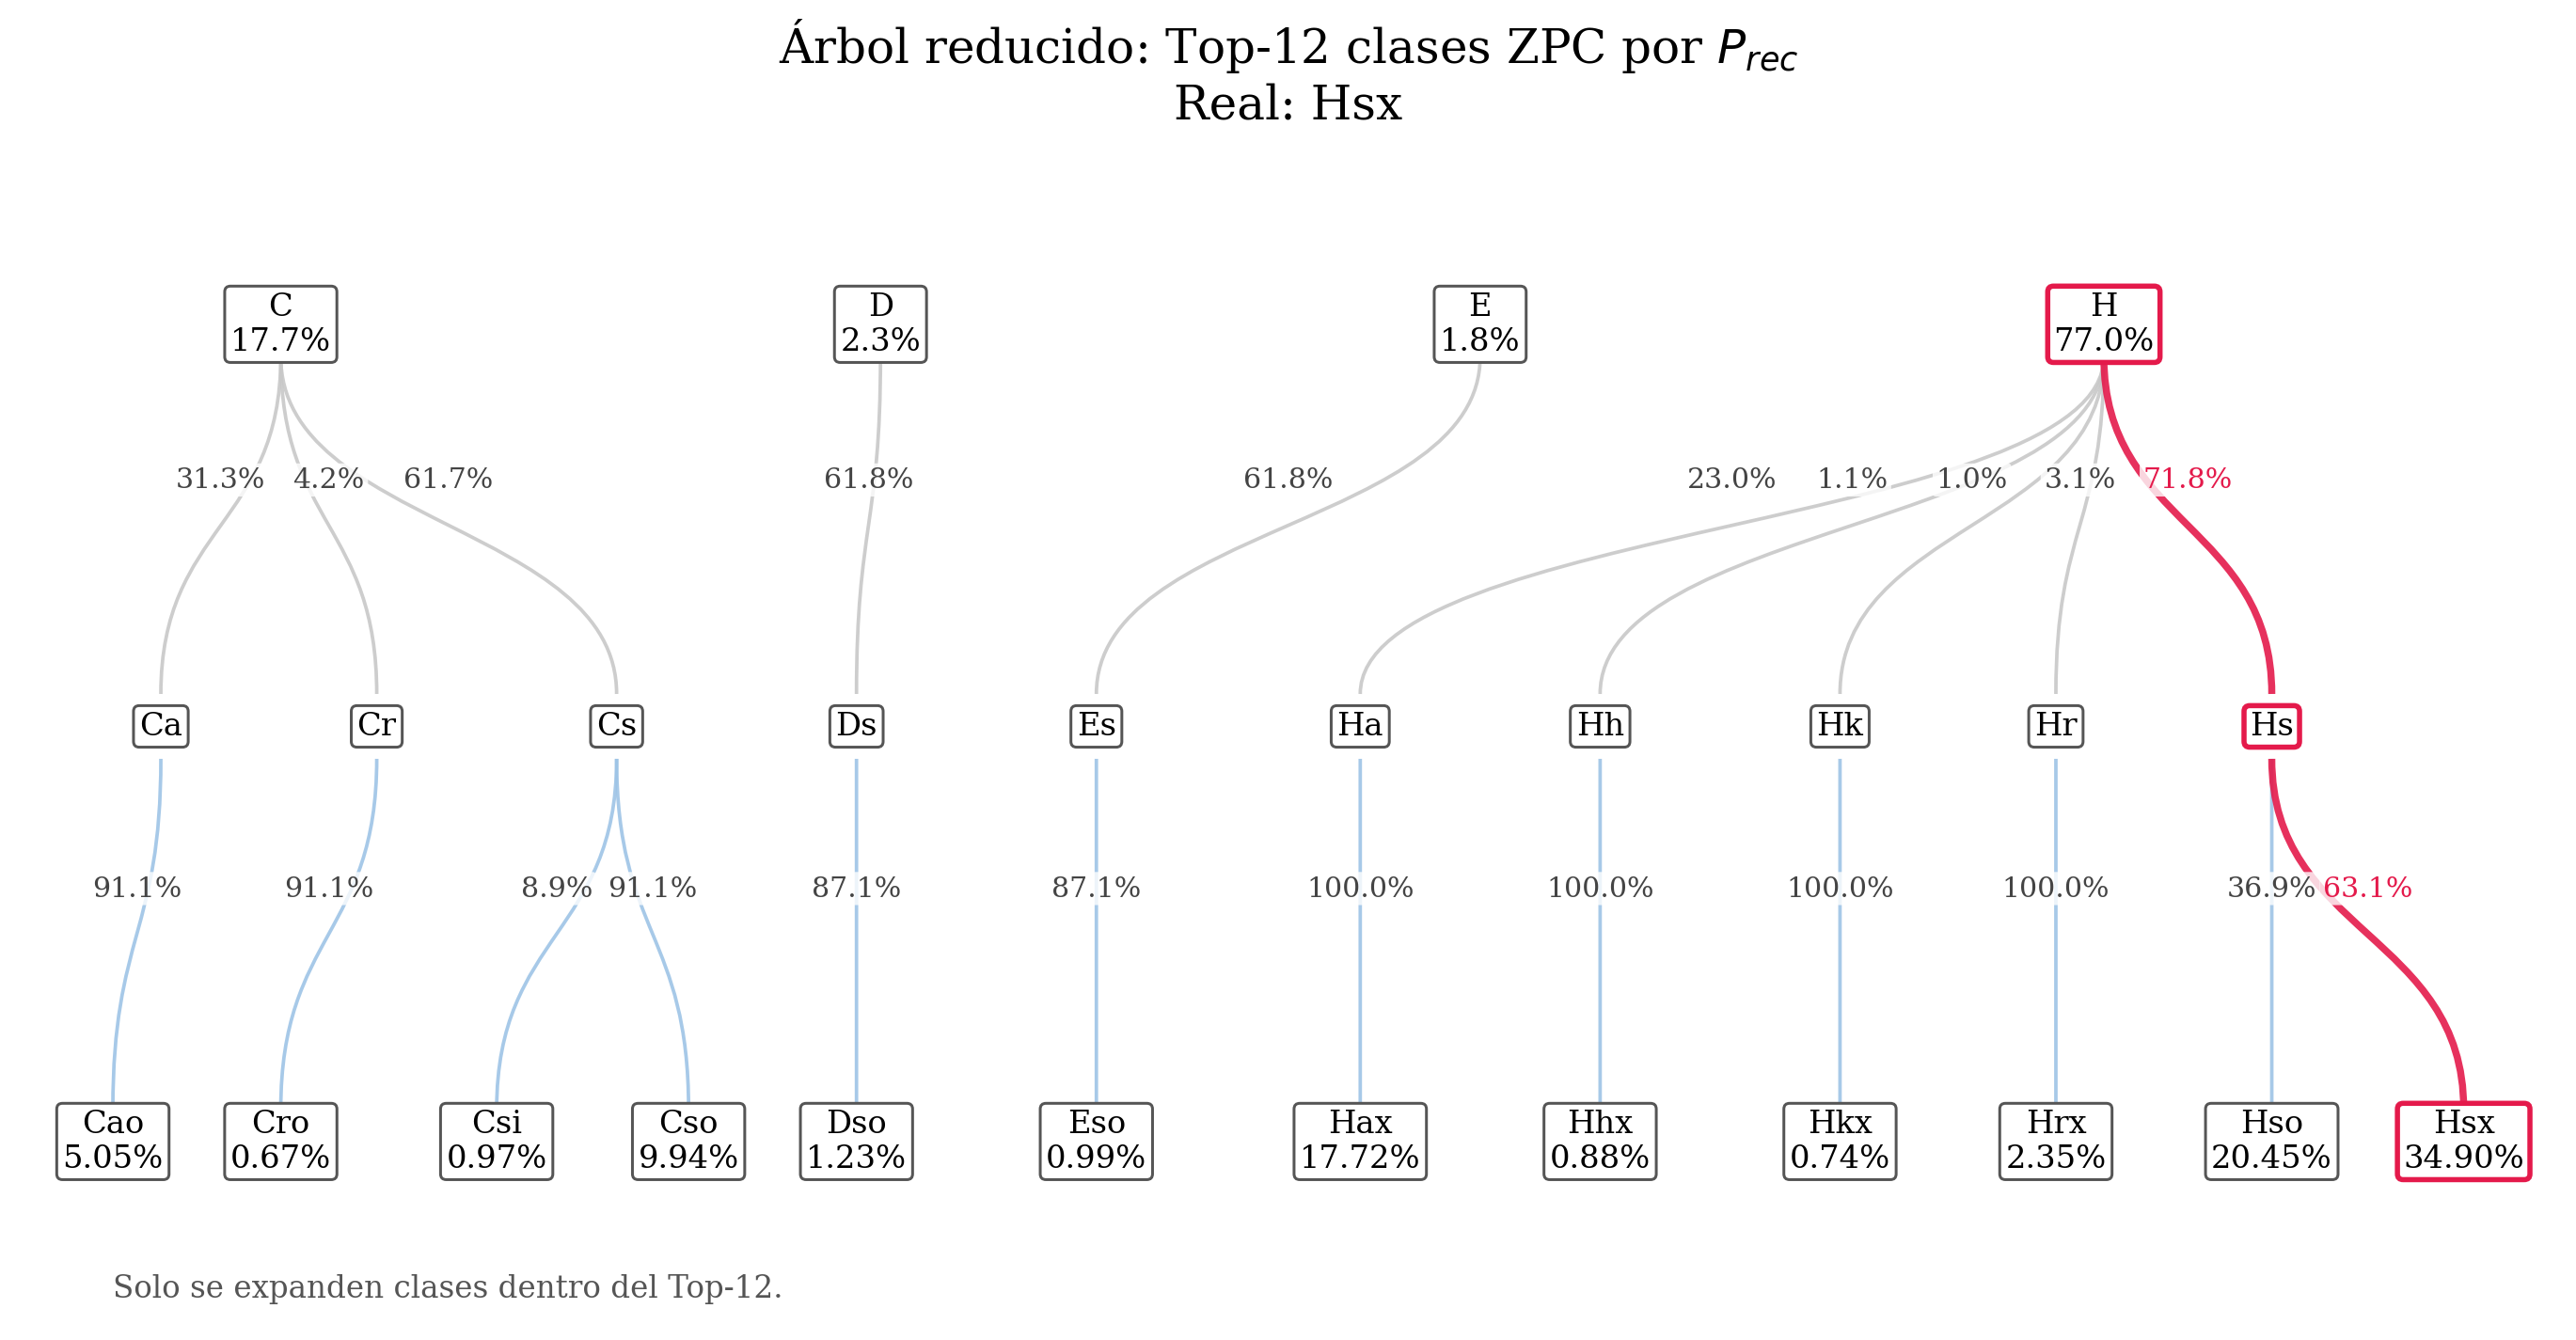
\includegraphics[width=0.92\textwidth]{figures/ml/top12_tree.png}
    \caption{Árbol bayesiano de probabilidades para la recomendación jerárquica
    Zurich--McIntosh. La visualización organiza las alternativas más probables
    según las componentes $Z$, $P$ y $C$, preservando la consistencia taxonómica
    de las clases válidas. \textbf{Fuente:} Elaboración propia.}
    \label{fig:resultados-arbol-top12-zpc}
\end{figure}

El árbol corresponde
a una implementación de los formalismos probabilísticos presentados en la
Sección~\ref{sec:classification}, donde la probabilidad conjunta se descompone de
forma jerárquica según las componentes $Z$, $P$ y $C$. Esta representación permite
inspeccionar cómo se distribuye la confianza desde el tipo de grupo $Z$ hacia las
componentes $P$ y $C$, y facilita identificar alternativas cercanas cuando existen
configuraciones morfológicamente similares.

La Figura~\ref{fig:resultados-top12-zpc} complementa esta lectura mediante un
histograma de las doce clases $ZPC$ con mayor probabilidad. El resultado muestra
que la masa probabilística se concentra en un subconjunto reducido de
combinaciones, mientras que las alternativas restantes presentan valores menores
pero todavía informativos. Este comportamiento es útil para un sistema de
asistencia observacional, ya que permite presentar una recomendación principal
junto con opciones secundarias ordenadas por plausibilidad, en lugar de forzar
una única etiqueta sin contexto de incertidumbre.

\begin{figure}[H]
    \centering
    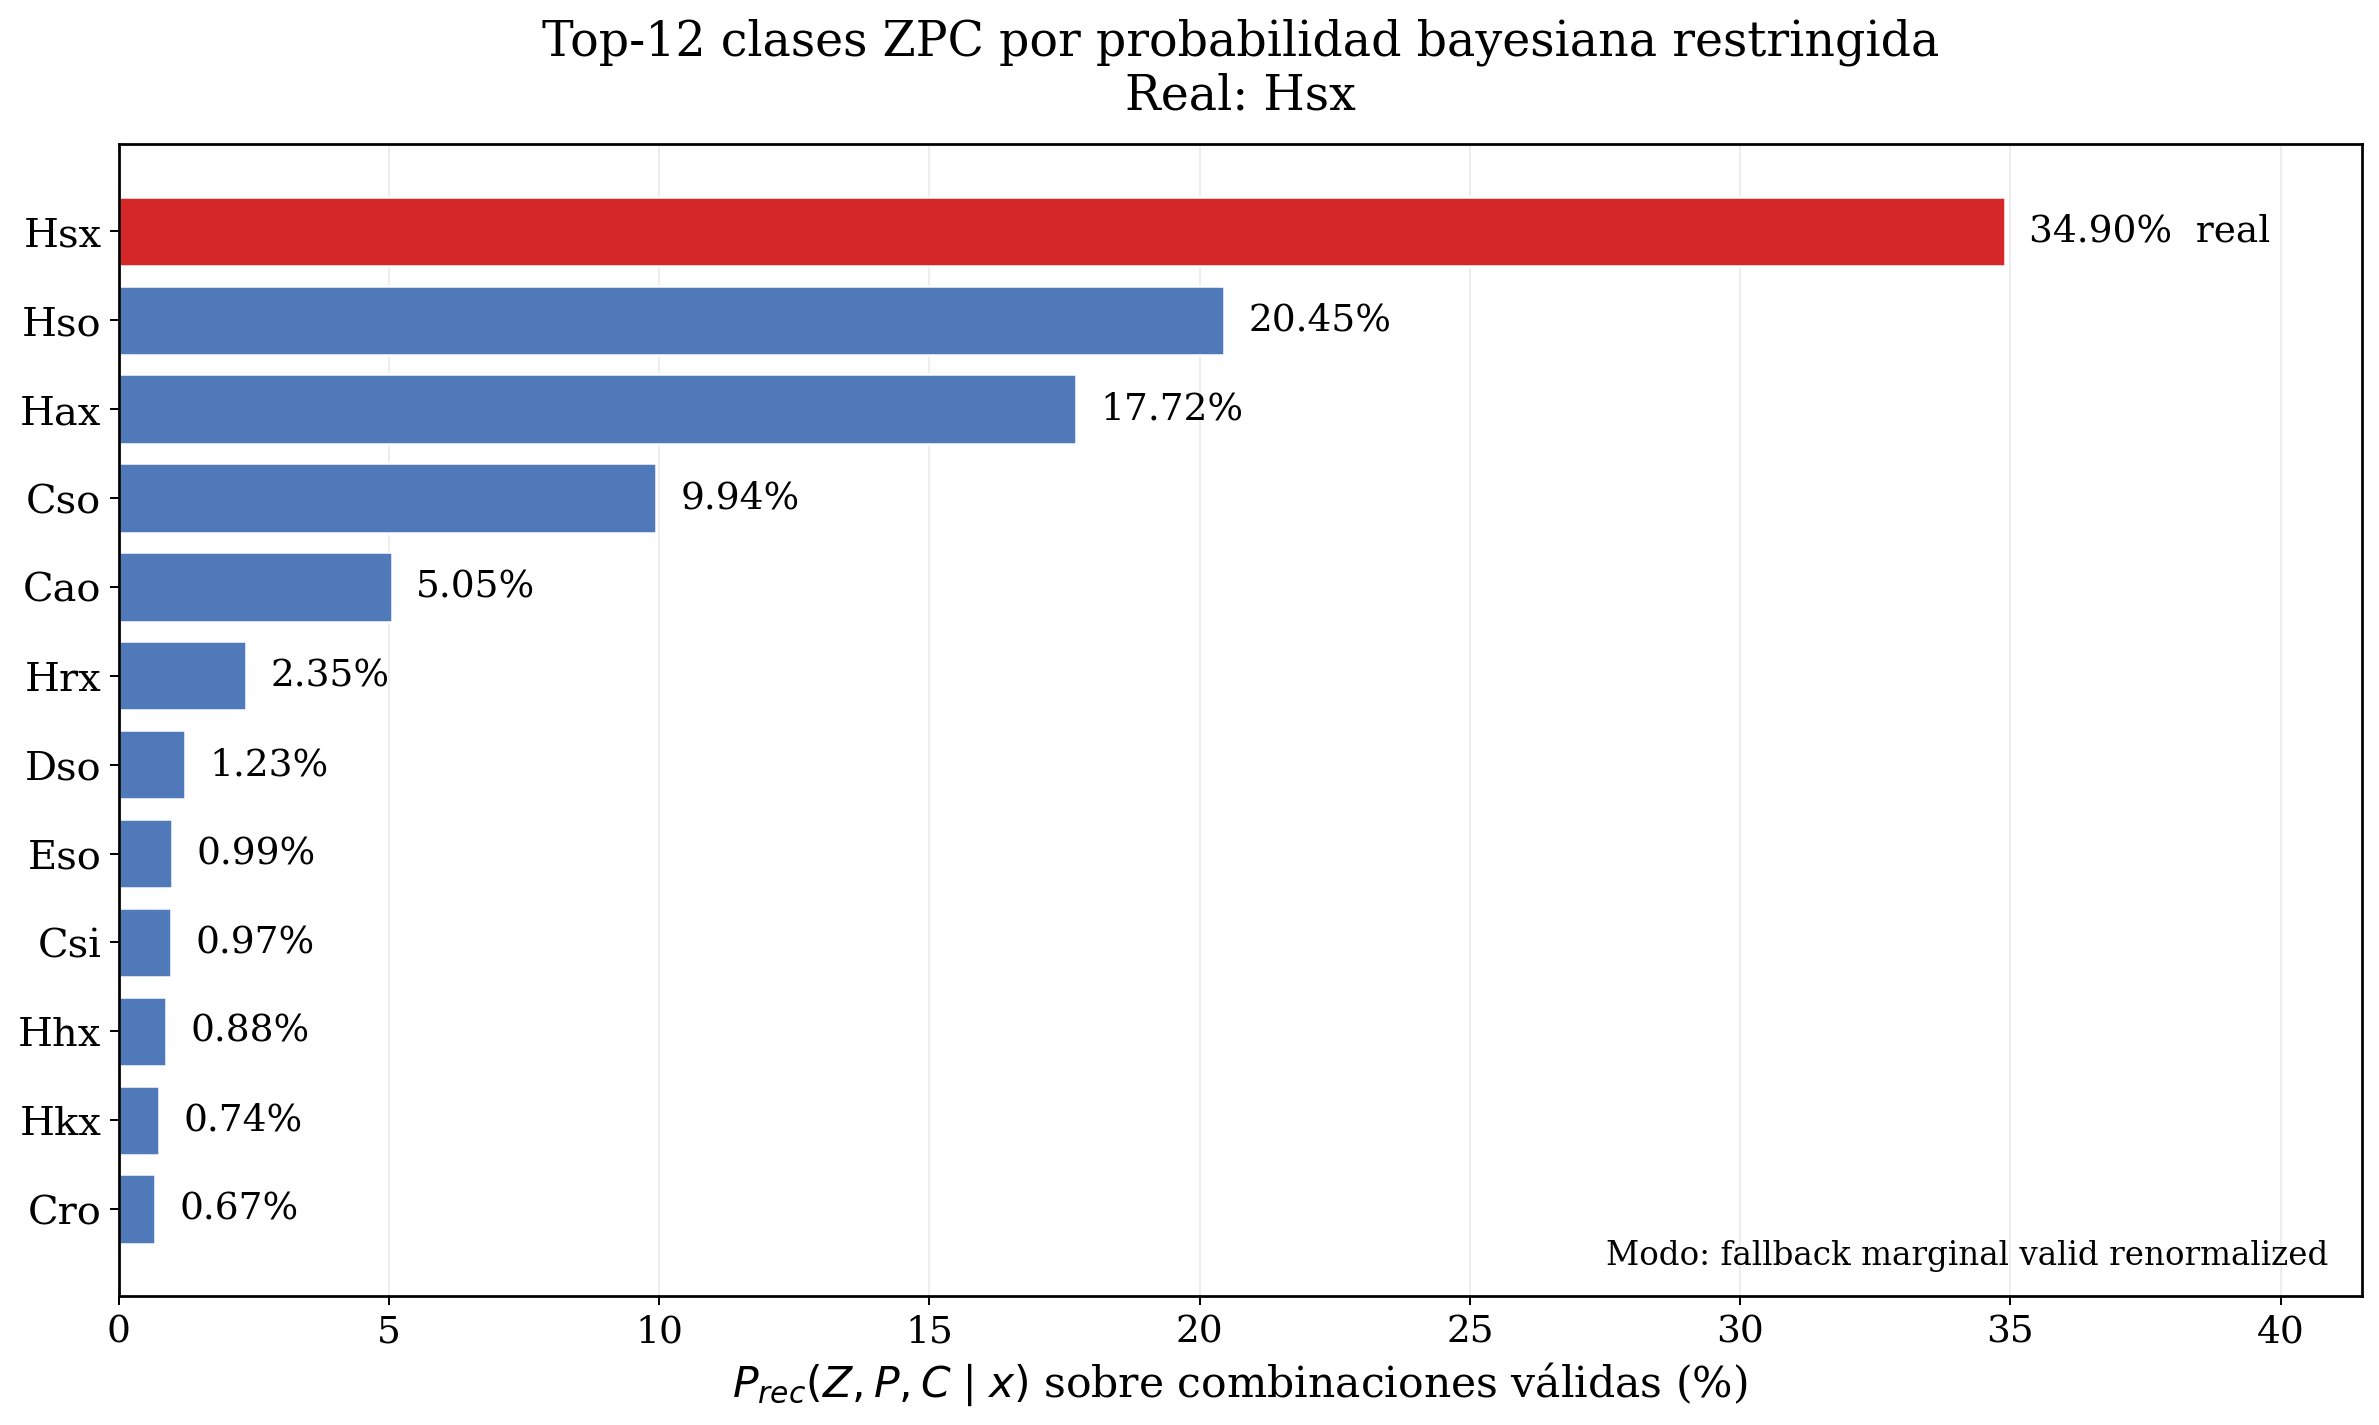
\includegraphics[width=0.92\textwidth]{figures/ml/top12_rec.png}
    \caption{Histograma del top 12 de clases Zurich--McIntosh recomendadas por
    probabilidad bayesiana restringida. La figura permite comparar la clase más
    probable con alternativas cercanas dentro del espacio válido de
    configuraciones $ZPC$. \textbf{Fuente:} Elaboración propia.}
    \label{fig:resultados-top12-zpc}
\end{figure}

Como síntesis comparativa, la Tabla~\ref{tab:comparativa-baselines} resume el
rendimiento por carácter bajo métrica F1 de trabajos representativos sobre
clasificación McIntosh, junto con la propuesta desarrollada en este manuscrito.

\begin{table}[H]
\centering
\caption{Comparación de F1-score para la clasificación McIntosh. Los valores
reportados se toman de las referencias correspondientes cuando están
disponibles. \textbf{Fuente:} Elaboración propia con base en la literatura citada.}
\label{tab:comparativa-baselines}
{\uniformtablestyle
\setlength{\tabcolsep}{7pt}
\begin{adjustbox}{center}
\begin{tabular}{lcccc}
\toprule
\textbf{Autor} & \textbf{F1-Z} & \textbf{F1-P} & \textbf{F1-C} & \textbf{F1 prom.} \\
\midrule
Palladino et al.\ (2022) \citep{palladino2022sunspot} & 0.67 & 0.55 & 0.72 & 0.65 \\
Sayez et al.\ (2023) \citep{sayez2023sunscc} & 0.68 & 0.65 & 0.72 & 0.68 \\
Deng et al.\ (2025) \citep{deng2025mcintosh} & 0.47 & 0.41 & 0.60 & 0.49 \\
Propuesta & 0.65 & 0.63 & 0.71 & 0.66 \\
\bottomrule
\end{tabular}
\end{adjustbox}
}
\end{table}

La propuesta alcanza un F1 promedio de $0.66$, valor próximo al mejor resultado
de referencia considerado en esta tesis ($0.68$). Esta comparación debe leerse
considerando la severidad de la métrica empleada: en este trabajo no se realiza
compactación artificial de clases ni se fusionan categorías raras para facilitar
la evaluación. Por el contrario, se conserva la taxonomía Zurich--McIntosh en sus
componentes originales, lo que obliga al modelo a distinguir diferencias sutiles
entre categorías cercanas, como $E$ y $F$ en la extensión longitudinal del grupo
o $C$ y $D$ en configuraciones bipolares compactas.

Desde esta perspectiva, mantener la granularidad taxonómica completa no se
considera una debilidad, sino una característica de diseño. Una clasificación
compactada podría elevar el F1 al reducir el número de fronteras difíciles, pero
también eliminaría información observacional útil para el usuario experto. La
propuesta privilegia una salida más estricta e interpretable, coherente con el
uso del sistema como herramienta de asistencia y revisión humana.

Más allá de los valores numéricos, las referencias comparadas responden a
decisiones metodológicas diferentes. Palladino et al.~\citep{palladino2022sunspot}
tratan cada componente ($Z$, $P$ y $C$) como un problema independiente.
Sayez et al.~\citep{sayez2023sunscc} proponen una arquitectura multitarea
jerárquica con ensamble y mecanismos adicionales de calibración de confianza.
Deng et al.~\citep{deng2025mcintosh} evalúan CNNs clásicas sobre particiones
más estrictas por región activa.

En contraste, la arquitectura desarrollada en esta tesis incorpora explícitamente
la dependencia jerárquica desde la salida $Z$ hacia las predicciones de $P$ y
$C$. Esta formulación preserva la semántica original de la taxonomía
Zurich--McIntosh y permite interpretar cada salida como una distribución de
probabilidad condicionada.

Los resultados también confirman que la componente $C$ es la de mejor
desempeño relativo, con un F1 de $0.71$, mientras que las mayores dificultades
se concentran en las componentes $Z$ y $P$, especialmente en clases con escaso
soporte muestral o fronteras morfológicas difusas. Este comportamiento es
consistente con las matrices de confusión analizadas en la Sección 5.2.2 y con
la distribución de cola larga observada en DB2.

En conjunto, estos resultados indican que la arquitectura jerárquica basada en
ConvNeXtV2 Atto logra un nivel de desempeño competitivo respecto al estado del
arte, manteniendo una estructura de salida interpretable y coherente con la
lógica observacional empleada por los catálogos Zurich--McIntosh. La elección de
la variante Atto respondió además a un criterio de despliegue: su tamaño reducido
favorece una conversión íntegra desde PyTorch hacia ONNX y facilita la ejecución
en entornos con recursos limitados. Las etapas MLP complementarias conservan el
aprendizaje jerárquico entre $Z$, $P$ y $C$ sin sacrificar la portabilidad de
las salidas.


\subsection{Resultados de los modelos predictivos}

La evaluación de los modelos predictivos se organiza en dos niveles complementarios. El primero corresponde al seguimiento escalar del número de manchas solares suavizado, denotado en la Sección~\ref{sec:forecast} como $\mathrm{SSN}_{\mathrm{PVLK}}(t_k)=\widehat{s}_k$, donde $\widehat{s}_k$ representa la estimación corregida del estado en el instante mensual $t_k$. El segundo corresponde a la reconstrucción espacio-temporal de la actividad latitudinal mediante DMD, donde el diagrama de Spörer se modela como una matriz de instantáneas $\mathbf{X}$ y su reconstrucción se denota por $\widehat{\mathbf{X}}$. Esta separación permite distinguir entre precisión de amplitud del ciclo y fidelidad en la migración latitudinal de la actividad.

Para la evaluación escalar se considera una secuencia observada $z_k$, asociada al SSN mensual suavizado, y una secuencia estimada $\widehat{s}_k$ generada por cada modelo en los mismos instantes $t_k$, con $k=1,\ldots,N$. A partir de estas dos series se calculan métricas de error absoluto, error cuadrático, error porcentual, ajuste global y correlación lineal. El error absoluto medio se define como
\begin{equation}
\mathrm{MAE}=\frac{1}{N}\sum_{k=1}^{N}\left|z_k-\widehat{s}_k\right|.
\end{equation}

La raíz del error cuadrático medio se calcula mediante
\begin{equation}
\mathrm{RMSE}=\sqrt{\frac{1}{N}\sum_{k=1}^{N}\left(z_k-\widehat{s}_k\right)^2}.
\end{equation}

El error porcentual absoluto medio se expresa como
\begin{equation}
\mathrm{MAPE}=\frac{100}{N}\sum_{k=1}^{N}\left|\frac{z_k-\widehat{s}_k}{z_k}\right|,
\end{equation}
siempre que $z_k\neq 0$ para los instantes considerados. El coeficiente de determinación se define como
\begin{equation}
R^2=1-\frac{\sum_{k=1}^{N}\left(z_k-\widehat{s}_k\right)^2}{\sum_{k=1}^{N}\left(z_k-\bar{z}\right)^2},
\end{equation}
donde $\bar{z}$ representa el promedio de la serie observada. Finalmente, la correlación de Pearson entre la serie observada y la estimada queda dada por
\begin{equation}
\rho=\frac{\sum_{k=1}^{N}\left(z_k-\bar{z}\right)\left(\widehat{s}_k-\bar{\widehat{s}}\right)}{\sqrt{\sum_{k=1}^{N}\left(z_k-\bar{z}\right)^2}\sqrt{\sum_{k=1}^{N}\left(\widehat{s}_k-\bar{\widehat{s}}\right)^2}},
\end{equation}
donde $\bar{\widehat{s}}$ es el promedio de la serie estimada.

Los resultados obtenidos para el periodo histórico se resumen en la Tabla~\ref{tab:ssn-metrics-comparison}. El modelo PVL--Kalman presenta el menor error absoluto y cuadrático, así como el mayor valor de $R^2$ y de correlación de Pearson. Esto indica que su formulación recursiva resulta particularmente adecuada para seguir la amplitud global del ciclo cuando el objetivo es aproximar la evolución temporal del SSN suavizado.

\begin{table}[H]
\centering
\caption{Comparativa de métricas de rendimiento para la predicción de SSN. \textbf{Fuente:} Elaboración propia basada en \texttt{ssn\_metrics.csv}.}
\label{tab:ssn-metrics-comparison}
\begin{tabular}{lccccc}
\hline
\textbf{Modelo} & \textbf{MAE} & \textbf{RMSE} & \textbf{MAPE (\%)} & \textbf{$R^2$} & \textbf{Pearson} \\ \hline
PVL--Kalman ($\mathrm{SSN}_{\mathrm{PVLK}}$) & 18.42 & 24.15 & 27.0 & 0.8942 & 0.9481 \\
DMD integral ($\mathrm{SSN}_{\mathrm{DMD}}$) & 22.15 & 29.84 & 33.0 & 0.8125 & 0.9104 \\ \hline
\end{tabular}
\end{table}

La evaluación del modelo DMD requiere métricas adicionales, porque su salida principal no es únicamente una serie escalar, sino una reconstrucción de la distribución latitudinal de la actividad. En este caso, $\mathbf{X}\in\mathbb{R}^{m\times N}$ representa la matriz observada de actividad latitudinal, donde cada columna corresponde a una instantánea mensual del diagrama de Spörer, y $\widehat{\mathbf{X}}$ representa la reconstrucción obtenida a partir del operador dinámico estimado. El error relativo de Frobenius se define como
\begin{equation}
E_F=\frac{\left\|\mathbf{X}-\widehat{\mathbf{X}}\right\|_F}{\left\|\mathbf{X}\right\|_F}.
\end{equation}

La coherencia espacio-temporal se evalúa mediante la correlación entre las matrices vectorizadas:
\begin{equation}
\rho_{ST}=\mathrm{corr}\left(\mathrm{vec}(\mathbf{X}),\mathrm{vec}(\widehat{\mathbf{X}})\right).
\end{equation}

Para medir la coherencia de la migración latitudinal se utiliza el error medio del centro latitudinal de actividad. Si $\theta_{c,k}$ es el centro latitudinal observado en el instante $t_k$ y $\widehat{\theta}_{c,k}$ su estimación reconstruida, entonces
\begin{equation}
\mathrm{MLCE}=\frac{1}{N}\sum_{k=1}^{N}\left|\theta_{c,k}-\widehat{\theta}_{c,k}\right|.
\end{equation}

La Tabla~\ref{tab:sporer-performance} resume los indicadores asociados a la reconstrucción latitudinal.

\begin{table}[H]
\centering
\caption{Métricas de reconstrucción espacio-temporal mediante DMD. \textbf{Fuente:} Elaboración propia basada en \texttt{sporer\_metrics.csv}.}
\label{tab:sporer-performance}
\begin{tabular}{lc}
\hline
\textbf{Métrica} & \textbf{Valor observado} \\ \hline
Error relativo de Frobenius ($E_F$) & 0.4473 \\
Correlación espacio-temporal ($\rho_{ST}$) & 0.8841 \\
Error medio del centro latitudinal (MLCE) & $4.80^{\circ}$ \\
Error en pendiente de migración & $0.31^{\circ}$/año \\ \hline
\end{tabular}
\end{table}


Aunque el error de Frobenius muestra que la reconstrucción no reproduce de manera exacta toda la intensidad de la matriz observada, la correlación espacio-temporal de $0.8841$ indica que la estructura global del patrón latitud--tiempo se conserva de forma consistente. Asimismo, el error medio del centro latitudinal de $4.80^{\circ}$ y el error de pendiente de migración de $0.31^{\circ}$/año sugieren que el desplazamiento medio de las bandas de actividad es capturado con una precisión adecuada para fines de análisis exploratorio.


Los resultados evidencian un compromiso entre precisión escalar y riqueza descriptiva. El modelo PVL--Kalman ofrece el mejor desempeño para estimar la amplitud del ciclo solar, con un MAPE de $27\%$, un $R^2$ de $0.8942$ y una correlación de Pearson de $0.9481$. Por tanto, constituye la alternativa más apropiada cuando el objetivo principal es seguir la evolución temporal del SSN suavizado dentro del flujo operacional del prototipo.

El modelo DMD, por su parte, presenta un error escalar mayor, pero aporta una salida que no puede obtenerse a partir de un modelo unidimensional: la reconstrucción de la estructura latitudinal de la actividad. Como se observa en la Figura~\ref{fig:sporer-migration-model}, esta formulación permite representar la aparición de bandas de actividad en latitudes medias y su desplazamiento progresivo hacia el ecuador, rasgo característico de la ley de Spörer. En consecuencia, su valor dentro del sistema no se limita a la predicción de una magnitud agregada, sino que reside en proporcionar una lectura espacio-temporal coherente con la dinámica del ciclo solar.

En síntesis, el filtro de Kalman adaptativo asociado al modelo PVL resulta más adecuado para el seguimiento escalar del índice SSN, mientras que el modelo DMD aporta una representación más informativa para analizar la distribución latitudinal de la actividad. Ambos enfoques cumplen funciones complementarias dentro del prototipo: el primero resume la amplitud temporal del ciclo y el segundo contextualiza espacialmente la evolución de la actividad fotosférica.

\subsection{Síntesis general de resultados experimentales (Deep Learning y modelos predictivos)}

Considerados en conjunto, los resultados obtenidos muestran que el prototipo
cumple satisfactoriamente los objetivos planteados. La etapa de agrupamiento
localiza regiones activas con precisión adecuada para el flujo posterior; la
clasificación jerárquica alcanza un desempeño competitivo respecto al estado
del arte; y los modelos predictivos aportan una capa complementaria de análisis
temporal y espacio-temporal.

Más allá de las métricas individuales, el principal aporte del trabajo radica en
la integración de estos componentes dentro de una arquitectura unificada que
abarca adquisición, almacenamiento, inferencia local y análisis asistido. En este
sentido, los resultados respaldan la viabilidad técnica del sistema como
herramienta de apoyo para observación solar en entornos académicos y
observatorios locales.

\section{Validación integral del sistema}

La validación del prototipo no se limitó al análisis de métricas cuantitativas,
sino que también consideró la operación coordinada de todos los componentes del
sistema: instrumentación óptica, adquisición local con Raspberry Pi 5,
persistencia de datos, inferencia local en el dispositivo (\textit{on-device}), plataforma web y generación
de resultados interpretables.

\subsection{Validación del hardware}

Una vez evaluados los módulos de agrupamiento, clasificación y predicción, la
validación integral requiere comprobar que dichos componentes pueden operar sobre
una plataforma física de adquisición y no solo sobre datos históricos o entornos
de entrenamiento. Por ello, la primera etapa de esta validación se centra en el
hardware que cierra el flujo experimental: captura óptica, atenuación solar,
adquisición con cámara astronómica, preprocesamiento local y acoplamiento al
instrumento del observatorio.

En este sentido, se documentó la integración física del sistema mediante
fotografías del módulo de observación, el acoplamiento de la cámara con el filtro
Herschel, el sensor de la ZWO ASI174MM Mini, la unidad de preprocesamiento local,
el hardware integrado del prototipo y su montaje sobre el telescopio. Esta
evidencia permite verificar que la arquitectura descrita en el Capítulo 5 fue
implementada sobre una configuración instrumental real, capaz de producir las
imágenes que alimentan las etapas posteriores de inferencia, almacenamiento y
visualización.

\begin{figure}[H]
    \centering
    \begin{subfigure}[t]{0.47\textwidth}
        \centering
        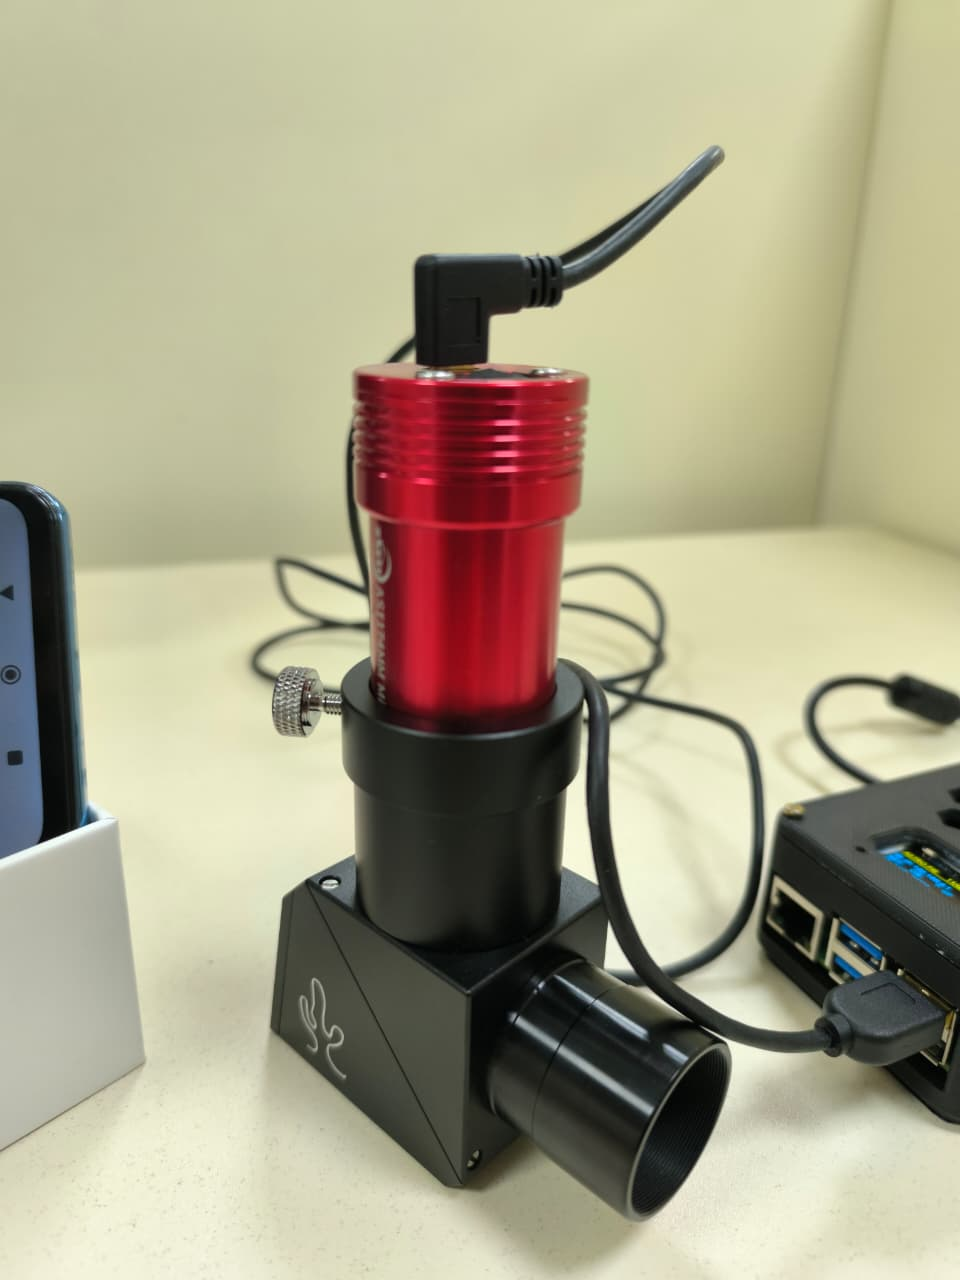
\includegraphics[width=\textwidth]{figures/hw/mount.jpeg}
        \caption{Montaje de la cámara ZWO ASI174MM Mini con el filtro Herschel.}
    \end{subfigure}
    \hfill
    \begin{subfigure}[t]{0.47\textwidth}
        \centering
        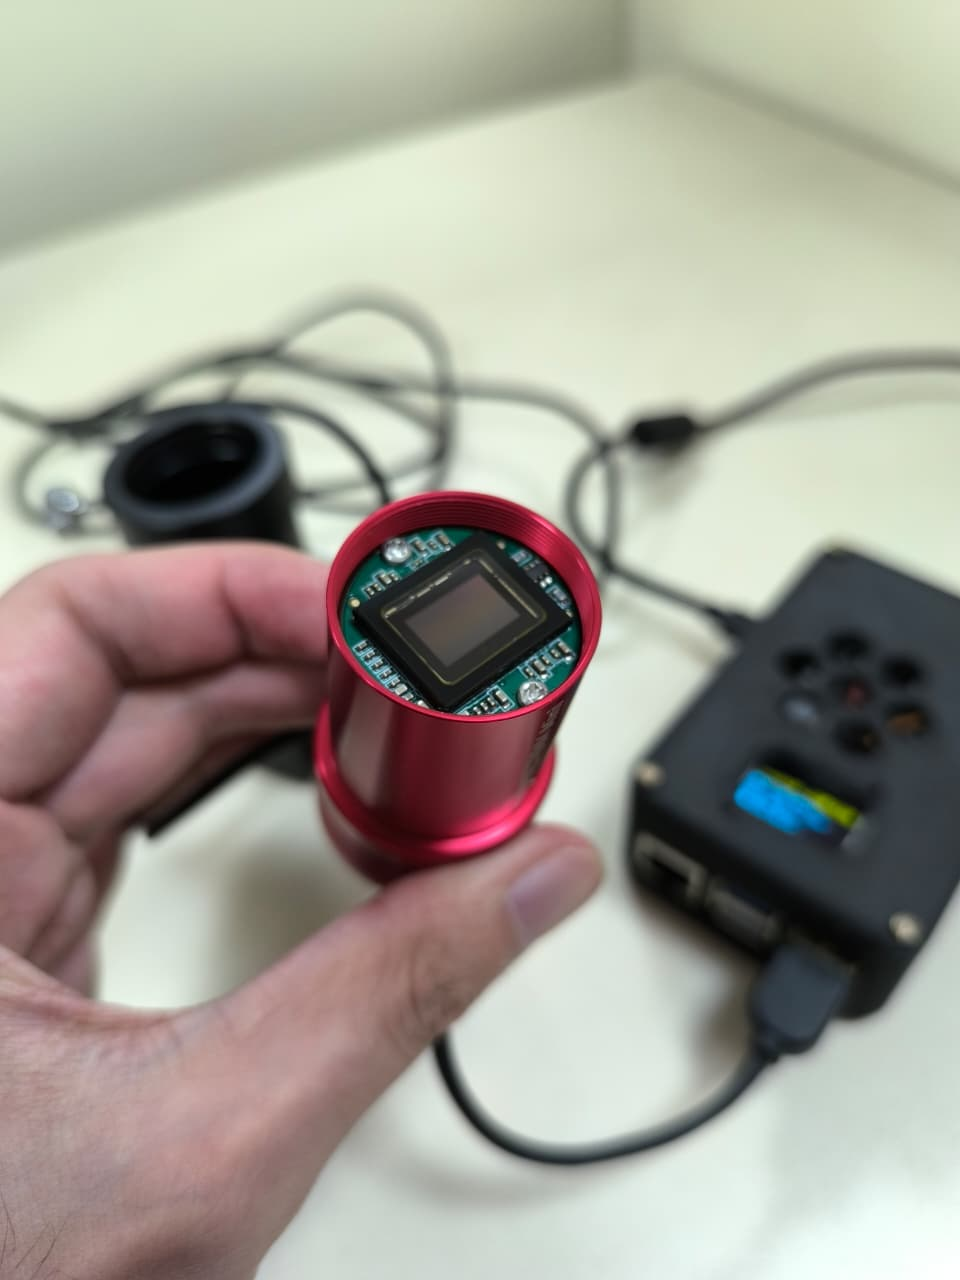
\includegraphics[width=\textwidth]{figures/hw/sensor.jpeg}
        \caption{Vista del sensor monocromático empleado para la adquisición.}
    \end{subfigure}
    \caption{Bloque de adquisición óptica empleado en la validación. Se muestran
    (a) el acoplamiento de la cámara con el filtro de atenuación solar y (b) el
    detalle del sensor de la cámara ZWO utilizado para la captura en luz blanca. \textbf{Fuente:} Elaboración propia.}
    \label{fig:camara-filtro-sensor-validacion}
\end{figure}

\begin{figure}[H]
    \centering
    \begin{subfigure}[t]{0.35\textwidth}
        \centering
        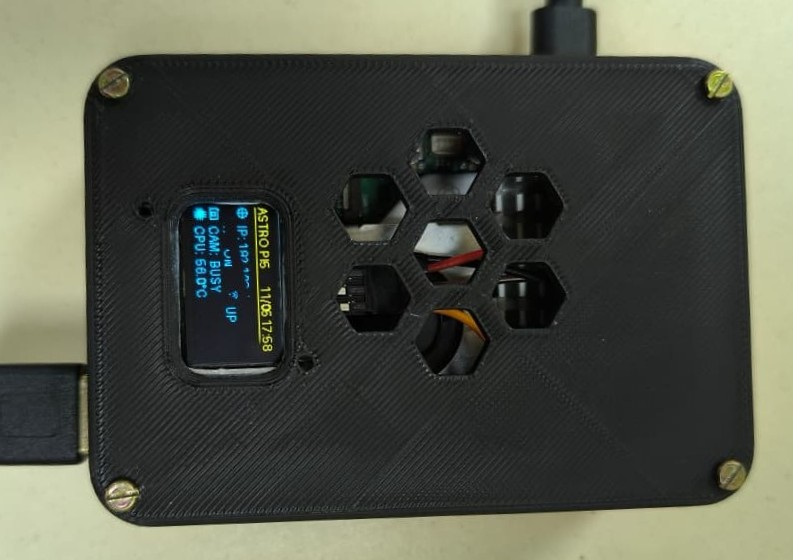
\includegraphics[width=\textwidth]{figures/hw/obs_module.jpeg}
        \caption{Módulo de preprocesamiento empleado durante las pruebas.}
    \end{subfigure}
    \hfill
    \begin{subfigure}[t]{0.6\textwidth}
        \centering
        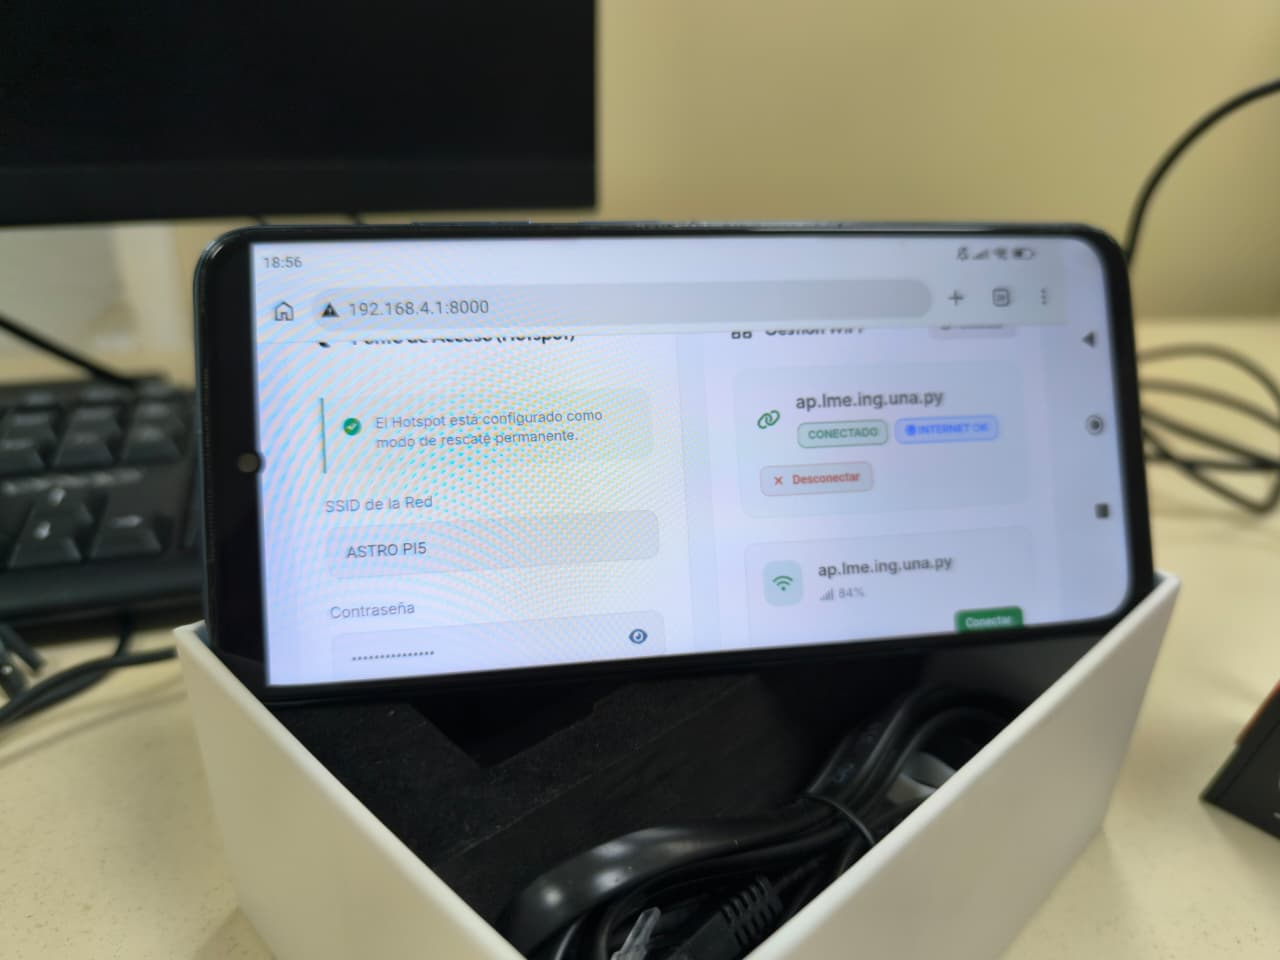
\includegraphics[width=\textwidth]{figures/hw/panel.jpeg}
        \caption{Acceso al panel local desde un dispositivo móvil.}
    \end{subfigure}
    \caption{Operación local de la unidad de preprocesamiento. Se muestran (a)
    el panel de control utilizado para supervisar el sistema y (b) el módulo
    desarrollado para integrar adquisición, preprocesamiento y conectividad. \textbf{Fuente:} Elaboración propia.}
    \label{fig:telefono-modulo-preprocesamiento-validacion}
\end{figure}

\begin{figure}[H]
    \centering
    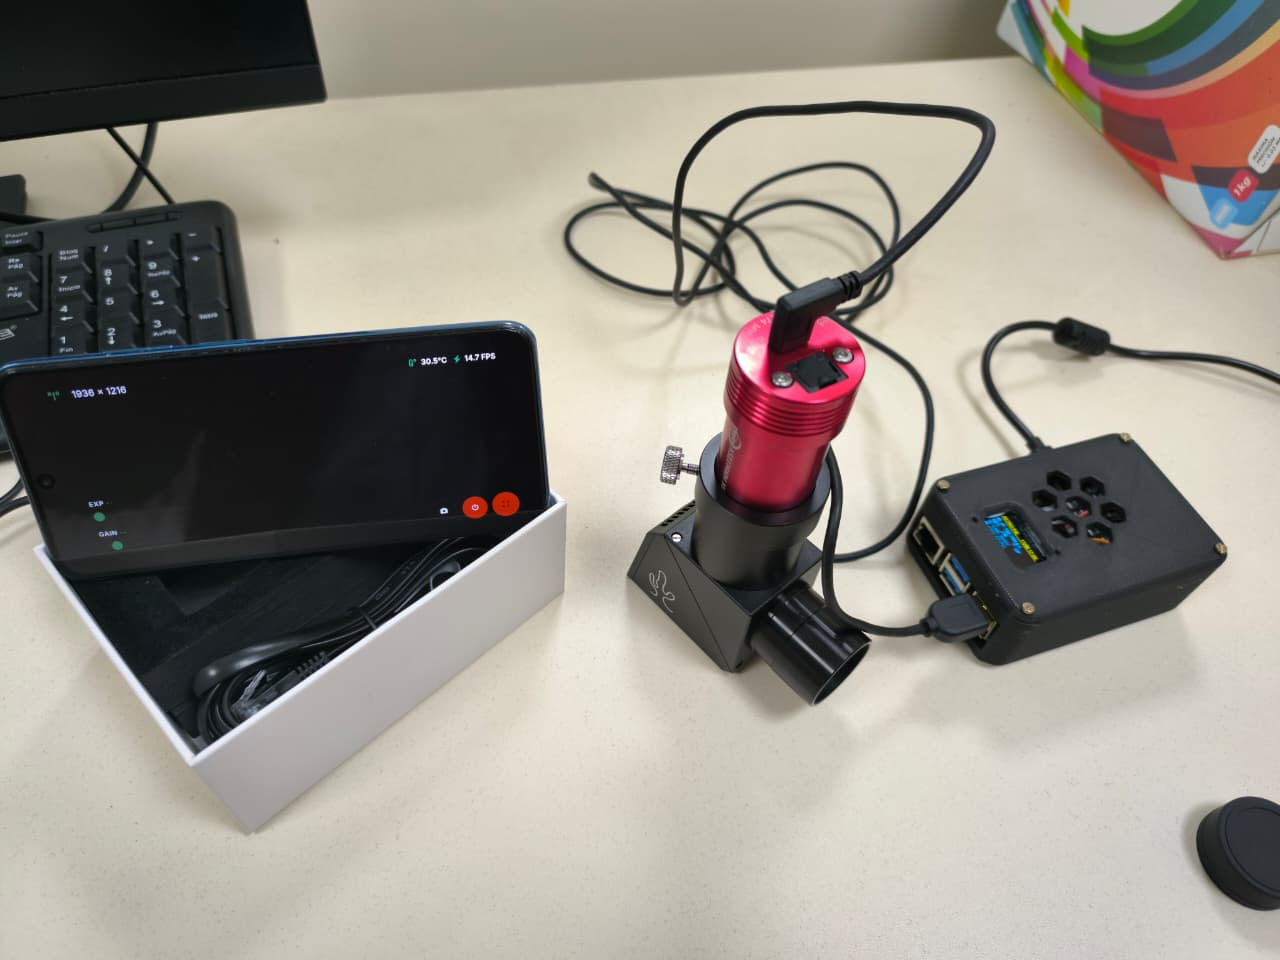
\includegraphics[width=0.72\textwidth]{figures/hw/integrated.jpeg}
    \caption{Hardware integrado del prototipo durante la etapa de validación,
    incluyendo la unidad de procesamiento local y los periféricos asociados. \textbf{Fuente:} Elaboración propia.}
    \label{fig:hardware-integrado-validacion}
\end{figure}

\begin{figure}[H]
    \centering
    \begin{subfigure}[t]{0.35\textwidth}
        \centering
        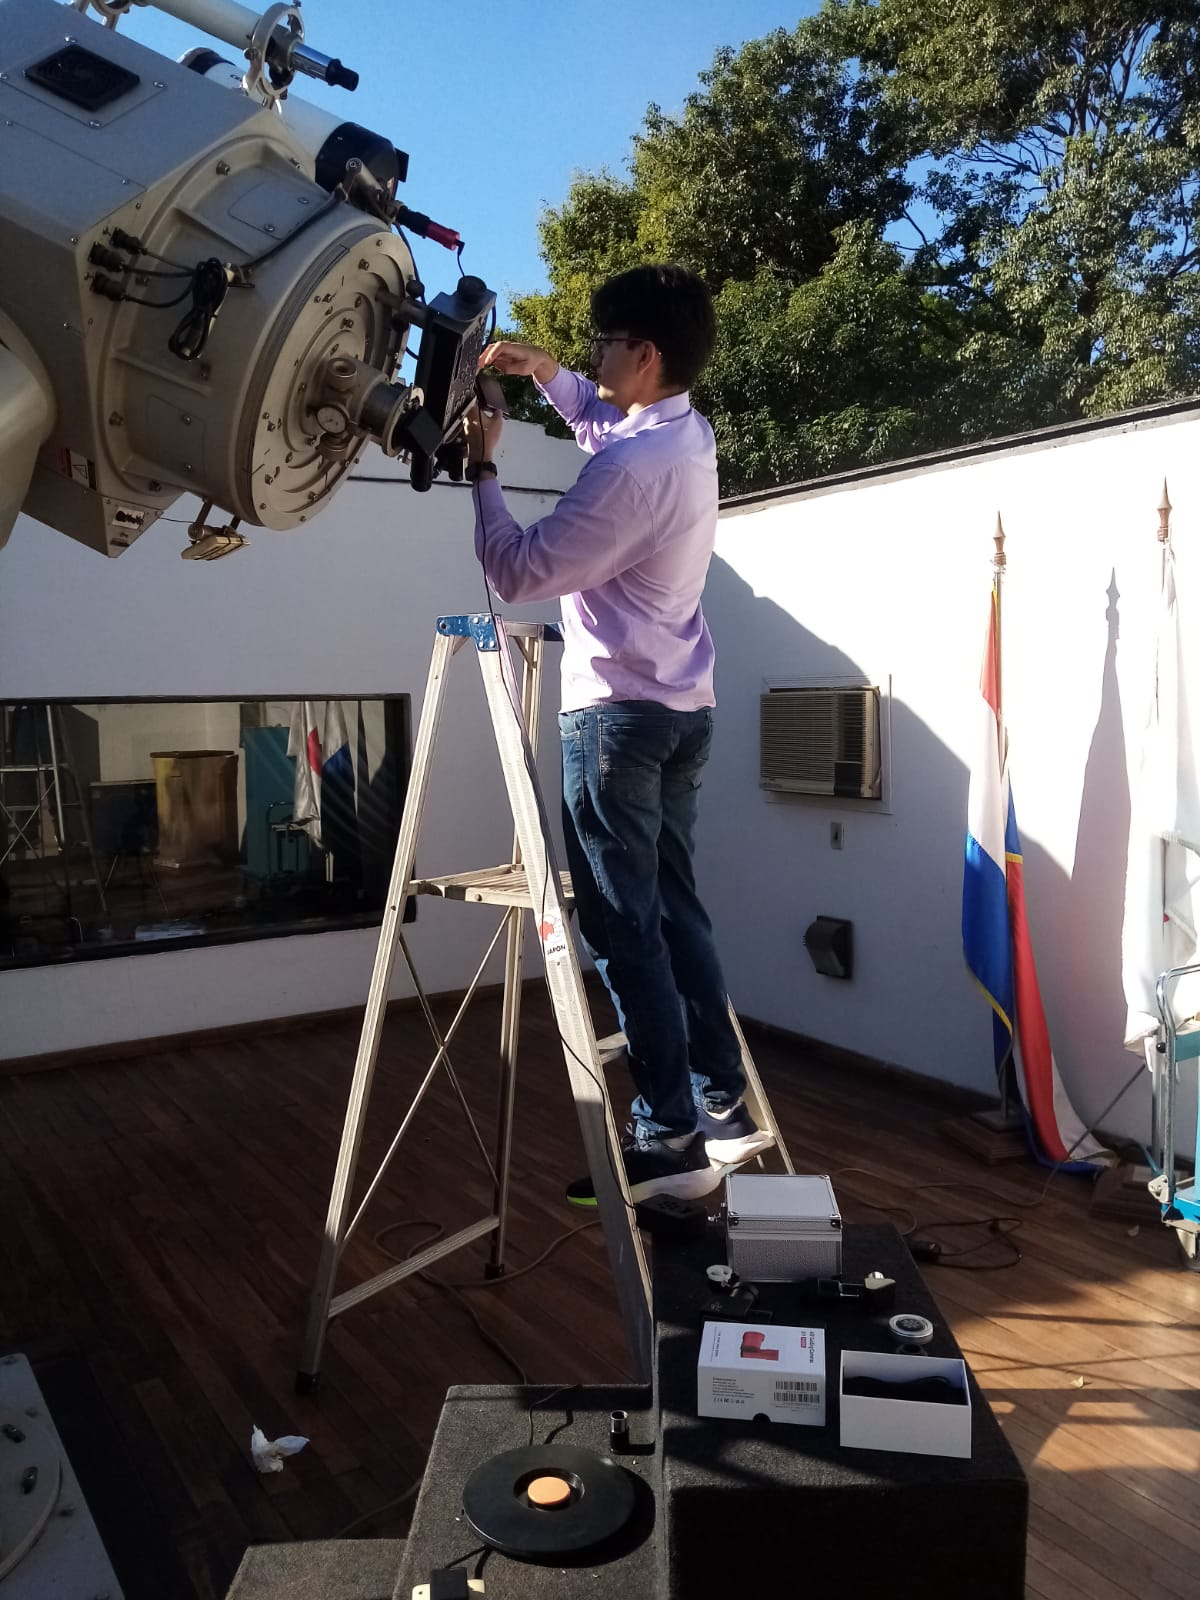
\includegraphics[width=\textwidth]{figures/hw/telescope.jpg}
        \caption{Telescopio del observatorio utilizado para las pruebas.}
    \end{subfigure}
    \hfill
    \begin{subfigure}[t]{0.6\textwidth}
        \centering
        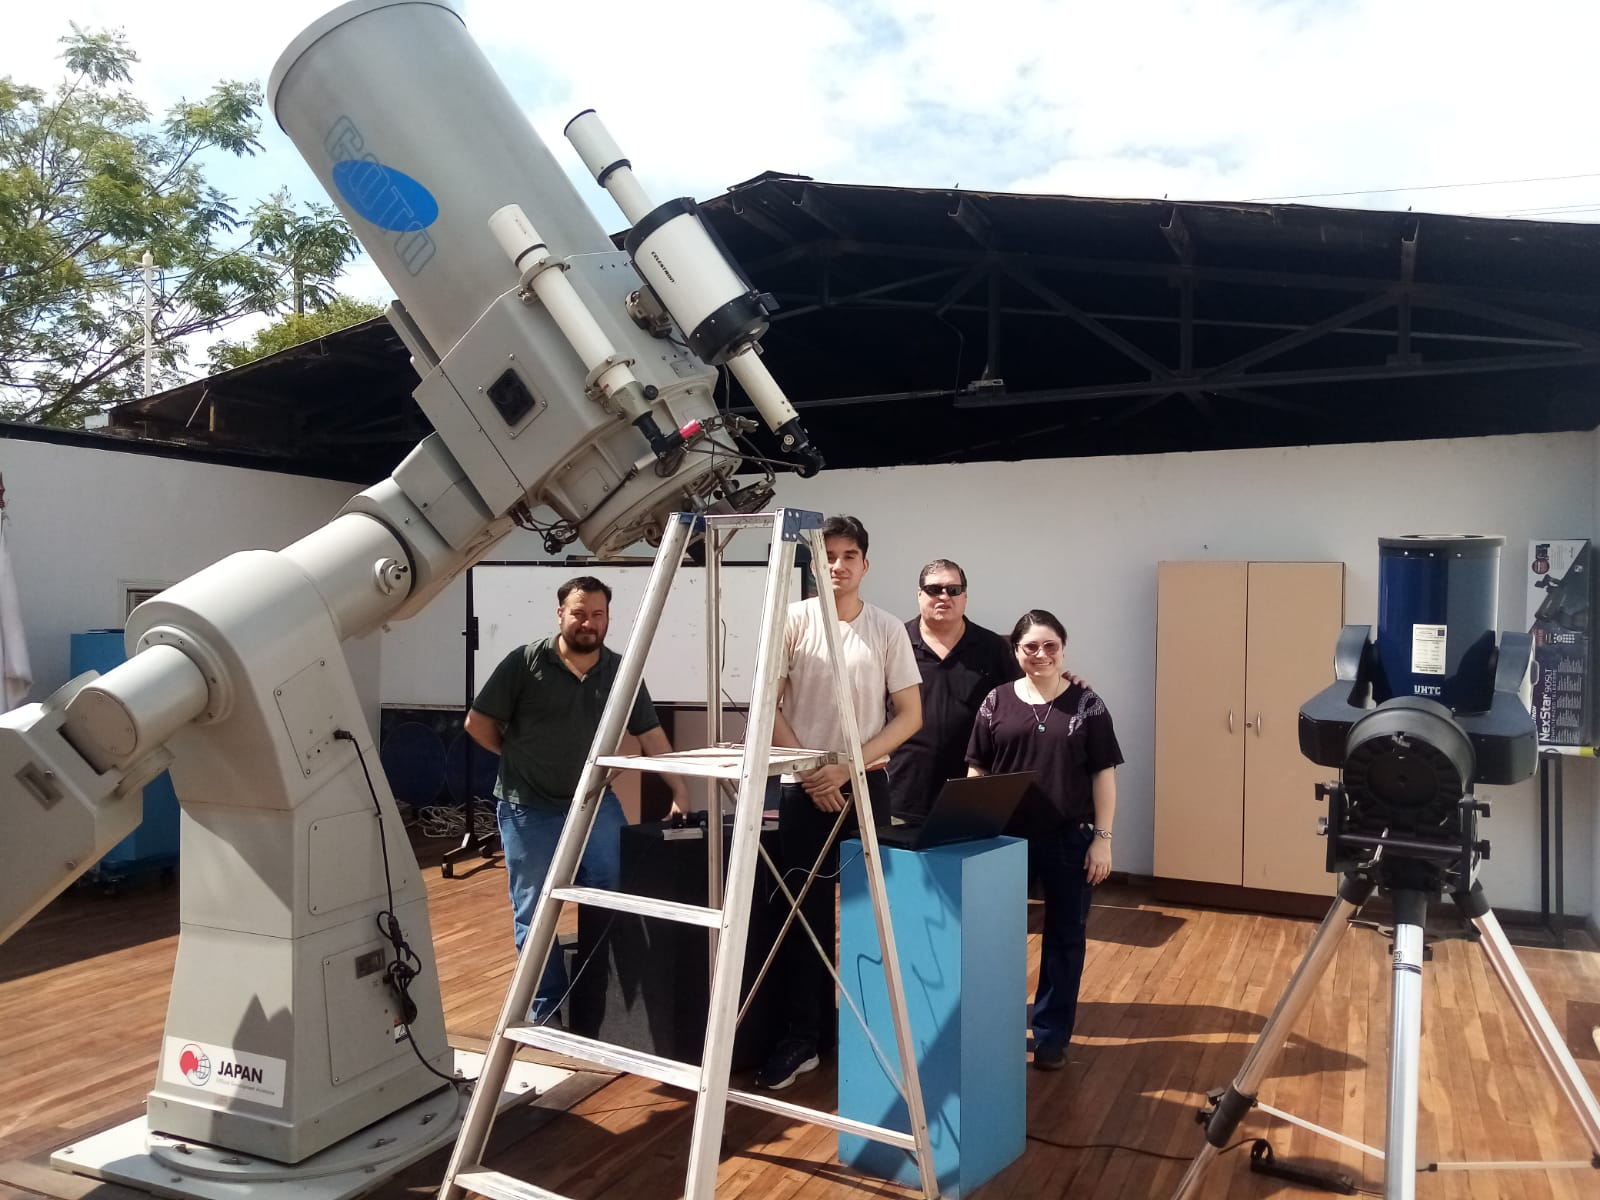
\includegraphics[width=\textwidth]{figures/hw/telescope_team.jpg}
        \caption{Integración del prototipo con el telescopio.}
    \end{subfigure}
    \caption{Integración del hardware con el telescopio del observatorio. Se
    muestran (a) el instrumento empleado para las pruebas y (b) el conjunto
    instalado para la validación del sistema completo. \textbf{Fuente:} Elaboración propia.}
    \label{fig:telescopio-integracion-validacion}
\end{figure}

\subsection{Métricas operativas en Raspberry Pi 5}

Además de verificar la integración física, se documentó una captura real
realizada el 2026-05-05 con el telescopio y el hardware de adquisición del
prototipo. La sesión se realizó bajo condiciones climáticas óptimas, con cielo
totalmente despejado, lo que favoreció la estabilidad de iluminación y la nitidez
de las capturas. Las imágenes resultantes fueron almacenadas en la base de datos
como parte del flujo operativo del sistema, permitiendo validar no solo la
obtención de la imagen, sino también su persistencia dentro de la infraestructura
de registro.

\begin{figure}[H]
    \centering
    \begin{subfigure}[t]{0.48\textwidth}
        \centering
        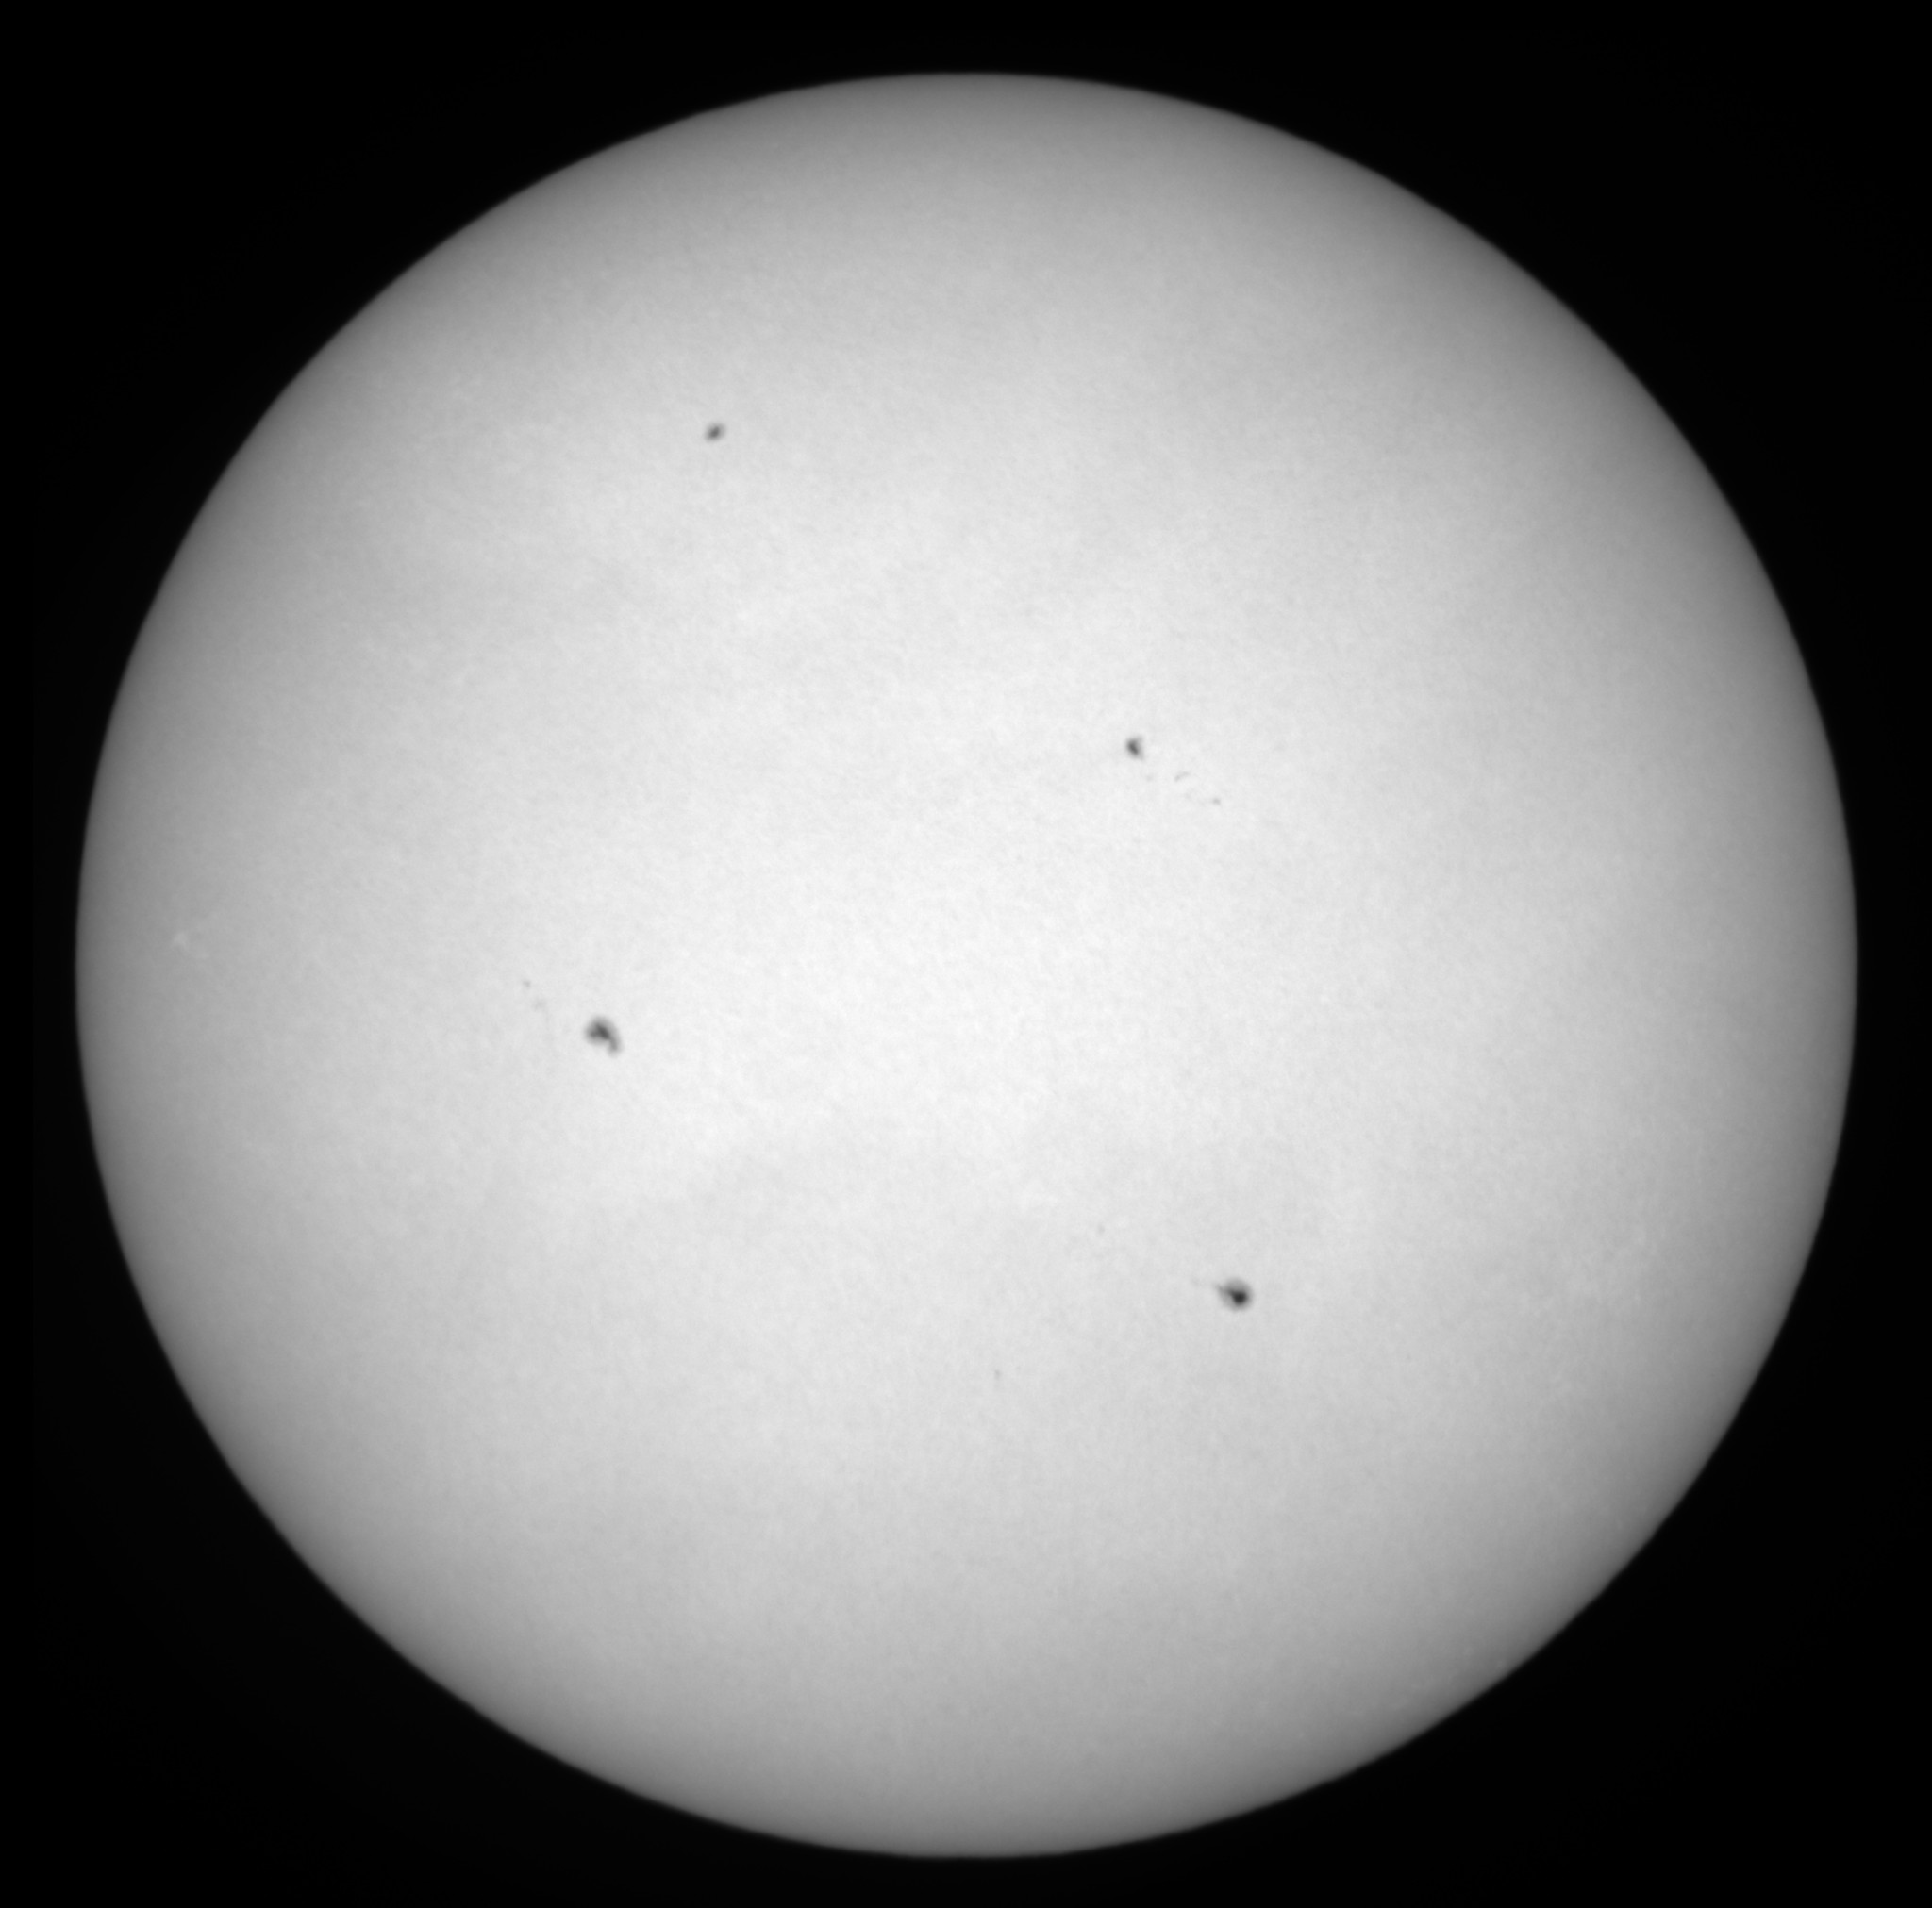
\includegraphics[width=\textwidth]{figures/obs/capture.jpg}
        \caption{Captura solar registrada durante la sesión del 2026-05-05.}
    \end{subfigure}
    \hfill
    \begin{subfigure}[t]{0.48\textwidth}
        \centering
        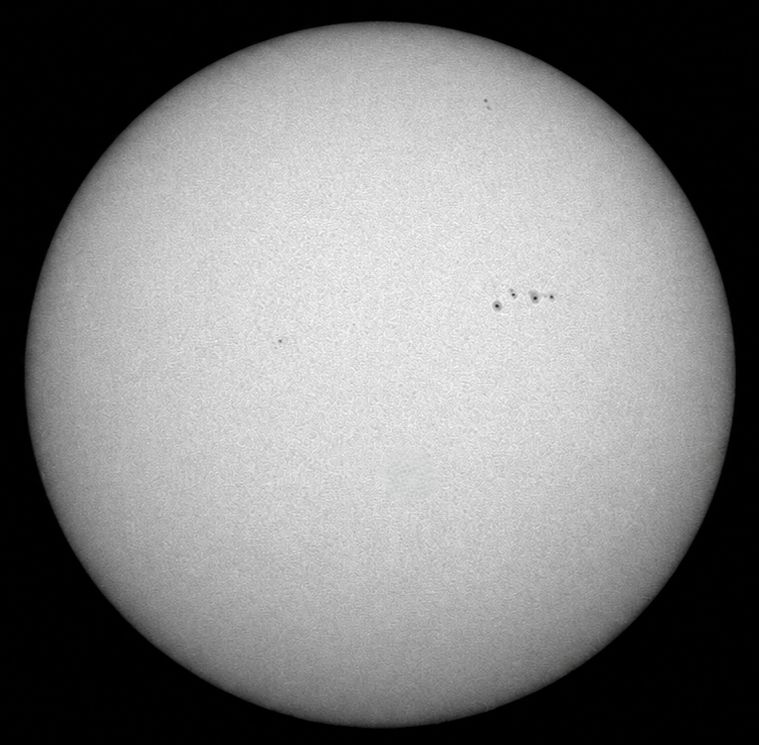
\includegraphics[width=\textwidth]{figures/obs/site.jpg}
        \caption{Imagen solar registrada el 20-05-2026 y almacenada en la base de datos del sistema.}
    \end{subfigure}
    \caption{Imágenes solares obtenidas mediante el telescopio y el hardware de
    adquisición del prototipo. \textbf{Fuente:} Elaboración propia.}
    \label{fig:capturas-solares-20260505-validacion}
\end{figure}

La Tabla~\ref{tab:parametros-captura-20260505} resume los parámetros de ajuste
empleados durante esta captura. La denominación \texttt{pi5-observatory}
corresponde al panel de interacción ejecutado en el servidor local de la
Raspberry Pi 5, desde el cual se controlan los parámetros de adquisición y se
coordina el registro de las observaciones.

\begin{table}[H]
\centering
\caption{Parámetros de adquisición utilizados durante la captura solar del
2026-05-05. \textbf{Fuente:} Elaboración propia.}
\label{tab:parametros-captura-20260505}
\uniformtablestyle
\begin{tabular}{ll}
\toprule
\textbf{Parámetro} & \textbf{Valor} \\
\midrule
Aplicación local & pi5-observatory \\
Versión & 1.0 \\
FPS & 15 \\
Temperatura del sensor & 36.7 °C \\
Binning & 1 \\
Ganancia & 1 \\
Ancho de imagen & 1936 px \\
Alto de imagen & 1216 px \\
Exposición & 500 us \\
\bottomrule
\end{tabular}
\end{table}

Además de esta evidencia de captura, se registraron métricas operativas de la
Raspberry Pi 5 durante sesiones típicas de adquisición, almacenamiento local y
sincronización remota. La Tabla~\ref{tab:metricas-raspberry-operacion} resume
valores representativos obtenidos con refrigeración activa, cámara ZWO ASI174MM
Mini y conexión WiFi disponible. Los tiempos de sincronización dependen del ancho
de banda efectivo, por lo que deben interpretarse como referencia de operación y
no como límite absoluto del sistema.

\begin{table}[H]
\centering
\caption{Métricas de rendimiento operativo del nodo Raspberry Pi 5 durante una sesión típica. \textbf{Fuente:} Elaboración propia.}
\label{tab:metricas-raspberry-operacion}
{\uniformtablestyle
\begin{tabular}{lc}
\toprule
\textbf{Métrica} & \textbf{Valor representativo} \\
\midrule
Tiempo de captura de imagen individual & 420 ms \\
Guardado local en almacenamiento microSD & 180 ms \\
Captura + guardado local & 600 ms \\
Preprocesamiento básico por imagen & 1350 ms \\
Sincronización a Supabase & 3800 ms/imagen \\
Uso medio de CPU en operación típica & 38\% \\
Uso máximo de CPU durante preprocesamiento & 72\% \\
Uso de RAM del servicio local & 3.3 GB \\
Temperatura tras sesión de 25 min & 57 °C \\
\bottomrule
\end{tabular}
}
\end{table}

Durante las pruebas no se observaron reinicios, cierres del servicio ni
reducción térmica perceptible bajo refrigeración activa. La temperatura se
mantuvo por debajo de umbrales críticos para la Raspberry Pi 5 y el uso de RAM
quedó dentro del margen disponible del modelo de 8 GB. Estos resultados respaldan
la viabilidad de operar el prototipo como nodo local de captura y asistencia,
siempre que se mantenga ventilación adecuada y se considere la variabilidad de la
red en la etapa de sincronización.

\subsection{Validación de la plataforma web}

Posteriormente, se verificó la operación desde la plataforma web actualizada. La
validación se concentró en el rendimiento percibido durante la carga de modelos,
la consulta de datos desde Supabase y la inferencia \textit{on-device} de los
módulos de agrupamiento y clasificación. Las capturas principales incluidas en
esta sección documentan las etapas funcionales del procesamiento y de la
visualización predictiva; las pantallas auxiliares de acceso, inicio y carga se
presentan como material complementario en el Anexo~\ref{anexo:suplementario}.

Para validar el flujo de inferencia visual en la plataforma, se empleó como caso
de prueba la imagen mostrada en la Figura~\ref{fig:capturas-solares-20260505-validacion}(b),
correspondiente a una captura solar del 2026-05-05 obtenida con el telescopio y
el hardware del prototipo, y posteriormente extraída desde la base de datos. A
partir de esta imagen se ejecutaron las etapas de agrupamiento y clasificación
\textit{on-device}, cuyos resultados se muestran en las Figuras~\ref{fig:web-yolo-validacion}
y~\ref{fig:web-convnextv2-validacion}.

\begin{figure}[H]
    \centering
    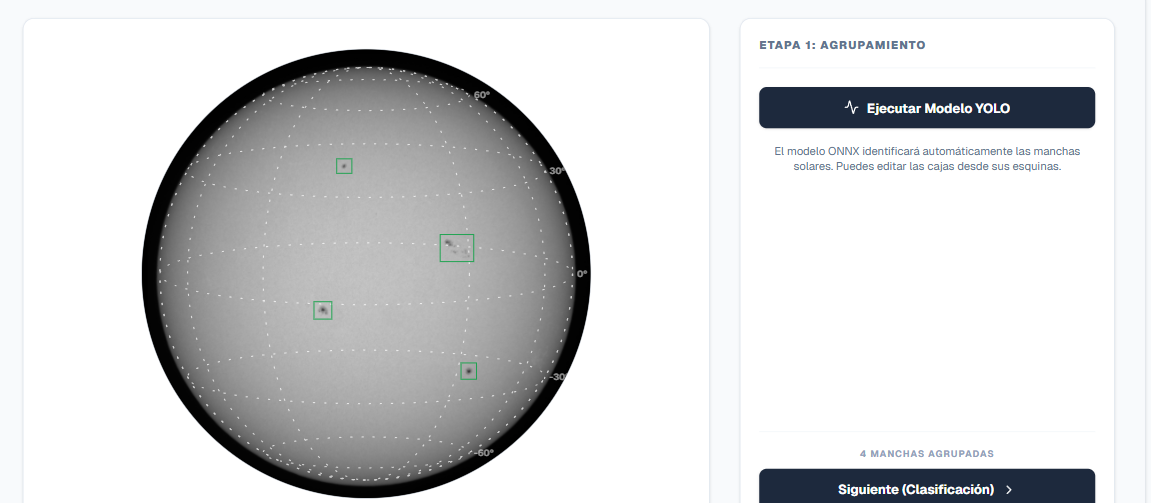
\includegraphics[width=0.82\textwidth]{figures/web/yolo.png}
    \caption{Etapa de agrupamiento \textit{on-device} aplicada a la imagen solar
    de la Figura~\ref{fig:capturas-solares-20260505-validacion}(b) mediante el
    modelo YOLO desplegado en la plataforma web. \textbf{Fuente:} Elaboración propia.}
    \label{fig:web-yolo-validacion}
\end{figure}

\begin{figure}[H]
    \centering
    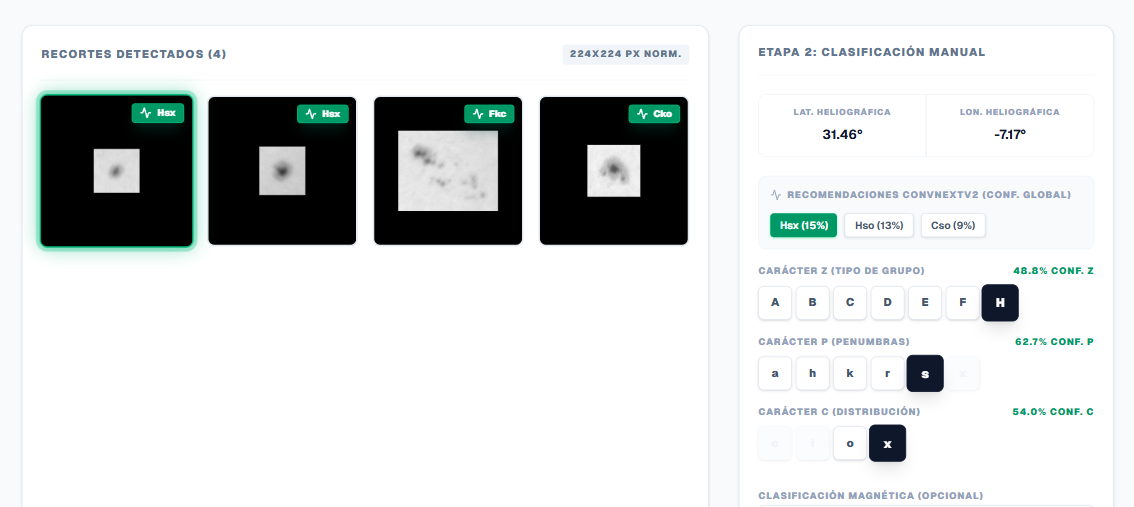
\includegraphics[width=0.82\textwidth]{figures/web/convnext.png}
    \caption{Etapa de clasificación morfológica \textit{on-device} aplicada a
    la imagen solar de la Figura~\ref{fig:capturas-solares-20260505-validacion}(b)
    mediante ConvNeXtV2 dentro de la plataforma web. \textbf{Fuente:} Elaboración propia.}
    \label{fig:web-convnextv2-validacion}
\end{figure}

\begin{table}[H]
\centering
\caption{Resultados de rendimiento de la plataforma web ejecutada en una
computadora personal. \textbf{Fuente:} Elaboración propia.}
\label{tab:rendimiento-plataforma-web-pc}
\uniformtablestyle
\begin{tabular}{ll}
\toprule
\textbf{Métrica} & \textbf{Valor} \\
\midrule
Dispositivo & Laptop ASUS TUF Gaming F15 \\
CPU & 12th Gen Intel(R) Core(TM) i5-12500H (2.50 GHz) \\
Núcleos simulados & 16 \\
CPU throttling & Nativo \\
Modo de red & Fibra / nativo \\
Velocidad de red & 780.0 Mbps / 585.0 Mbps \\
Proveedor de ejecución & \texttt{executionProviders: ["wasm"]} \\
Tiempo de descarga del modelo & 5803 ms \\
Tiempo de galería Supabase & 1702 ms \\
Inferencia YOLO & 3105 ms \\
Inferencia de clasificación & 3201 ms \\
\bottomrule
\end{tabular}
\end{table}

Aunque el equipo de prueba dispone de una GPU NVIDIA GeForce RTX 3050 Laptop GPU
de 4 GB y de gráficos integrados Intel(R) Iris(R) Xe Graphics de 128 MB, la
ejecución de los modelos se condicionó al proveedor \texttt{wasm}. Esta decisión
evita utilizar aceleración por GPU durante la inferencia y permite aproximar el
comportamiento esperado en dispositivos de recursos más limitados, donde el
procesamiento debe sostenerse principalmente mediante CPU y WebAssembly.

Además del procesamiento visual, la plataforma integra módulos predictivos para
consultar la evolución temporal del número de manchas solares y la distribución
latitudinal de la actividad. Estos módulos no operan sobre una captura individual,
sino sobre series históricas y reconstrucciones espacio-temporales, por lo que
complementan la clasificación morfológica con una lectura de tendencia solar.

\begin{figure}[H]
    \centering
    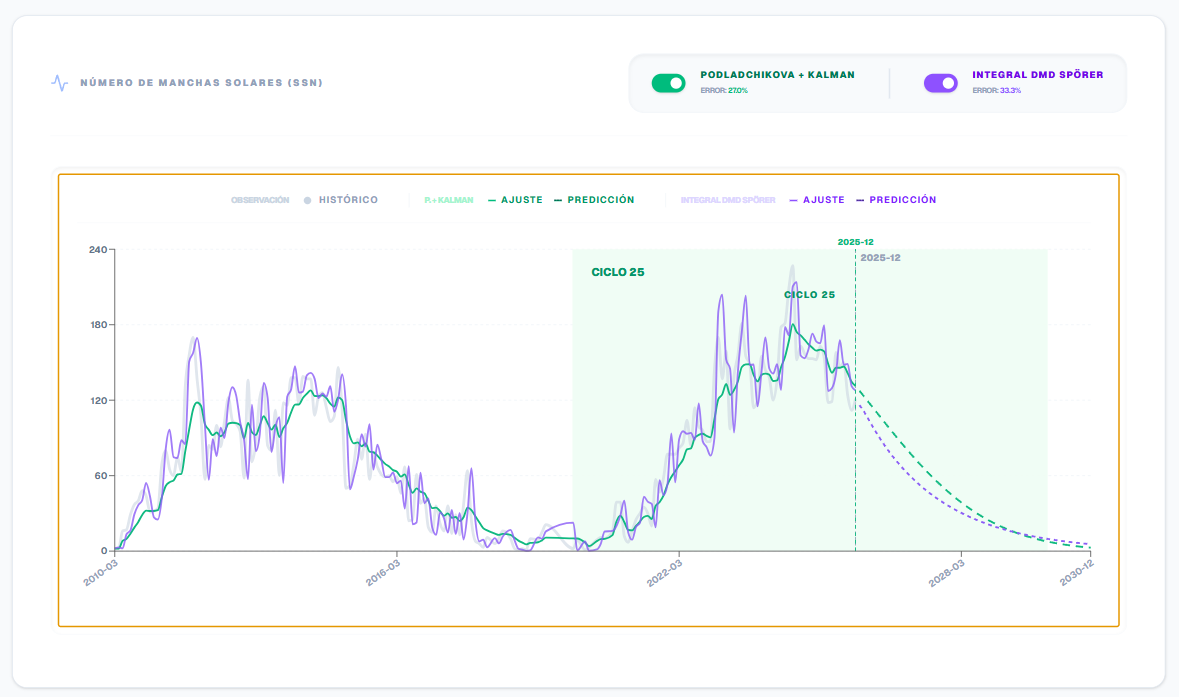
\includegraphics[width=0.82\textwidth]{figures/web/ssn.png}
    \caption{Módulo de predicción temporal del número de manchas solares
    integrado en la plataforma web. \textbf{Fuente:} Elaboración propia.}
    \label{fig:web-ssn-prediccion-validacion}
\end{figure}

\begin{figure}[H]
    \centering
    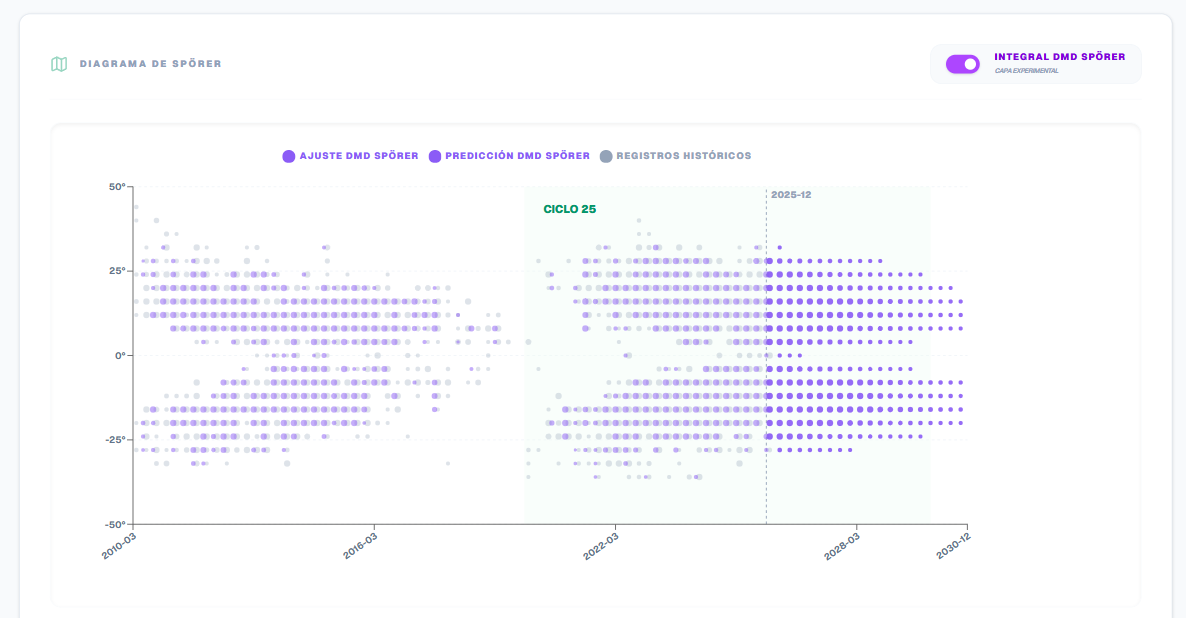
\includegraphics[width=0.82\textwidth]{figures/web/butterfly.png}
    \caption{Visualización del diagrama de mariposa para analizar la
    distribución latitudinal de la actividad solar. \textbf{Fuente:} Elaboración propia.}
    \label{fig:web-diagrama-mariposa-validacion}
\end{figure}

En términos funcionales, la validación confirma que el sistema puede capturar
imágenes, registrar metadatos, ejecutar inferencia local mediante modelos ONNX
y almacenar los resultados en la base de datos sin intervención manual
significativa. Los modelos ONNX exportados pesan en conjunto aproximadamente
24~MB, un tamaño adecuado para descarga, sincronización y actualización en
entornos de conectividad limitada. Esta evidencia respalda la consistencia
operativa del prototipo y demuestra que la solución propuesta trasciende el
entrenamiento aislado de modelos para constituirse en una plataforma de
asistencia observacional integrada.


\section{Análisis de Costos e Inversión del Proyecto}

La implementación del prototipo requirió una inversión directa asociada a los
componentes principales de adquisición, atenuación óptica, procesamiento local,
visualización de estado y soporte físico. La Tabla~\ref{tab:presupuesto-prototipo}
resume el presupuesto referencial empleado para construir la configuración
validada.

\begin{table}[H]
\centering
\caption{Presupuesto referencial de componentes principales del prototipo. Los montos en guaraníes se estiman con un tipo de cambio referencial de 1 USD = 6108 PYG. \textbf{Fuente:} Elaboración propia.}
\label{tab:presupuesto-prototipo}
\uniformtablestyle
\begin{tabularx}{\textwidth}{>{\raggedright\arraybackslash}X r r}
\toprule
\textbf{Componente} & \textbf{Precio USD} & \textbf{Precio PYG} \\
\midrule
Raspberry Pi 5 8 GB & 190 & 1160520 \\
Módulo active cooler para Raspberry Pi 5 & 13 & 79404 \\
Cámara ZWO ASI174MM Mini & 432 & 2638656 \\
Filtro solar Herschel wedge Lunt 1.25'' con ND3 & 308 & 1881264 \\
Pantalla OLED 0.96'' 128x64 & 9 & 54972 \\
Impresión 3D de carcasa y soporte & 4 & 24432 \\
\midrule
\textbf{Total} & \textbf{956} & \textbf{5839248} \\
\bottomrule
\end{tabularx}

\end{table}

El costo total estimado del prototipo fue de US\$956, equivalente a
5,839,248 PYG bajo el tipo de cambio referencial utilizado en la tabla. Este
monto incluye los elementos indispensables para disponer de una estación local de
captura solar en luz blanca: unidad de procesamiento, refrigeración, cámara,
cuña de Herschel, pantalla de estado y soporte impreso en 3D. La mayor parte de
la inversión se concentra en la cámara monocromática y el sistema de atenuación
solar, componentes críticos para preservar calidad de imagen y seguridad óptica.

El proyecto fue financiado parcialmente por el programa de becas PUBIABM, que
cubrió el 70\% del costo total del prototipo. Este esquema de financiamiento permitió reducir la carga económica
directa de implementación y facilitó la adquisición de componentes de mayor
impacto técnico sin comprometer la reproducibilidad del sistema.

Desde el punto de vista de inversión, el prototipo mantiene una relación
favorable entre costo y funcionalidad. La selección de Raspberry Pi 5 evita
recurrir a estaciones de trabajo dedicadas para la etapa de captura; el uso de
software abierto y modelos exportados a ONNX reduce dependencias de licencias o
servidores de inferencia; y la carcasa impresa en 3D disminuye costos de
integración mecánica. Además, varios componentes pueden reutilizarse en futuras
campañas observacionales o en extensiones del sistema, por lo que la inversión no
se limita a una única sesión de validación. Al finalizar el trabajo, todos los
elementos adquiridos serán donados al Observatorio Astronómico ``Prof.~Alexis
Troche Boggino'', de modo que queden disponibles para continuidad operativa,
formación académica y otros proyectos afines de observación solar o desarrollo
instrumental.

\section{Limitaciones de la validación actual}

Aunque los resultados obtenidos son consistentes con los objetivos del trabajo,
la validación presenta algunas restricciones. La principal limitación radica en el
tamaño y distribución de los conjuntos de datos, especialmente en clases poco
frecuentes de la taxonomía Zurich--McIntosh. Asimismo, la evaluación en campo
se realizó sobre un número acotado de sesiones observacionales y bajo una
configuración instrumental específica. Esta restricción se ve reforzada por el
hecho de que las observaciones óptimas dependen de condiciones climáticas
favorables, cuya variabilidad dificulta significativamente la adquisición, y por
el rango horario limitado en el que el Sol es observable desde el observatorio.

Por otra parte, los modelos predictivos deben interpretarse como herramientas
de apoyo para el análisis exploratorio y no como sistemas operacionales de
pronóstico solar. Su utilidad principal radica en complementar la interpretación
temporal de la actividad observada.

Estas limitaciones no invalidan los resultados presentados, pero delimitan el
alcance de las conclusiones y señalan oportunidades claras para trabajos
futuros orientados a ampliar la base de datos, incorporar observaciones
adicionales y refinar los modelos desarrollados.
\chapter[Discusión y conclusiones]{Discusión y conclusiones\label{cap:discusion}}

\section{Discusión}

\label{sec:discussion}

El desarrollo presentado en esta tesis debe interpretarse como la integración de
un flujo observacional completo, y no únicamente como la suma de modelos de
aprendizaje profundo evaluados de forma aislada. A lo largo del trabajo se
articulan decisiones instrumentales, criterios de construcción de datos,
modelos de visión por computadora, herramientas predictivas y mecanismos de
despliegue local y web, siguiendo la arquitectura metodológica formulada en el
Capítulo~\ref{cap:consideraciones}, implementada en el Capítulo~\ref{cap:software}
y validada en el Capítulo~\ref{cap:resultados}. Esta perspectiva resulta importante
porque el problema de análisis automático de manchas solares no se limita a
reconocer patrones en una imagen: exige capturar observaciones de manera
reproducible, asociarlas con metadatos físicos, preservar trazabilidad, ejecutar
inferencia en condiciones de campo y ofrecer resultados interpretables para el
usuario.

Desde el punto de vista instrumental, la selección de una cadena óptica basada en
observación de luz blanca, cámara monocromática y atenuación mediante cuña de
Herschel responde a un compromiso entre seguridad, resolución, portabilidad y
viabilidad operativa. La ZWO ASI174MM Mini ofrece un sensor de área suficiente,
píxeles relativamente grandes, obturador global y compatibilidad práctica con
entornos Linux, rasgos adecuados para una estación de observación local. La
Raspberry Pi 5, por su parte, permite concentrar adquisición, preprocesamiento,
conectividad y servicios locales en una unidad compacta. Esta combinación,
discutida en el diseño instrumental y validada físicamente en el
Capítulo~\ref{cap:resultados}, no pretende competir con observatorios solares
profesionales, sino demostrar que un observatorio académico o local puede
incorporar una capa de asistencia computacional moderna sin requerir
infraestructura de gran escala \citep{zwoASI174Manual2025,luntWhiteLightWedges2026,raspberryPi5Docs2026}.

La discusión de hardware también revela una restricción central del sistema: la
calidad de la inferencia depende de la estabilidad de la adquisición. Condiciones
como el \textit{seeing}, la nubosidad, el enfoque, la exposición y la ganancia de
la cámara condicionan la nitidez de umbra y penumbra, y por tanto afectan tanto
la detección de grupos como la clasificación morfológica. Por ello, el
preprocesamiento local, el control de parámetros de captura y la verificación de
estado mediante panel local no son accesorios secundarios, sino componentes
necesarios para sostener la calidad de los datos que alimentan los modelos. Esta
lectura es coherente con las limitaciones de validación señaladas en el
Capítulo~\ref{cap:resultados}, donde se reconoce que las campañas observacionales
están condicionadas por clima, ventana horaria solar y estabilidad instrumental.

En relación con los datos de entrenamiento, una de las decisiones metodológicas
más relevantes fue utilizar imágenes SDO/HMI acopladas con reportes NOAA SRS para
construir conjuntos etiquetados, como se detalla en la
Sección~\ref{sec:data-software}. Esta elección se justifica por la disponibilidad
temporal, la regularidad instrumental y la existencia de metadatos taxonómicos
asociados \citep{scherrer2012hmi,noaaSRS}. Sin embargo, también introduce
una tensión metodológica: el sistema
final está orientado a imágenes de luz blanca obtenidas localmente, mientras que
el entrenamiento se apoya en una modalidad espacial fotosférica distinta. La
similitud morfológica entre HMI y luz blanca permite sostener esta aproximación
como punto de partida razonable, pero no elimina la necesidad de validar la
transferencia entre instrumentos. En consecuencia, los resultados obtenidos deben
leerse como una validación funcional y metodológica del flujo, no como una
caracterización definitiva del rendimiento sobre todos los escenarios de
observación terrestre.

La separación entre agrupamiento y clasificación constituye otro aspecto central
de la propuesta. Esta estrategia en cascada fue formalizada en la
Sección~\ref{sec:arquitectura-dl-cascada} e implementada en la
Sección~\ref{sec:training}. El detector YOLO26n opera sobre imágenes de disco
completo y tiene como objetivo localizar grupos solares, mientras que el
clasificador basado en ConvNeXtV2 Atto trabaja sobre recortes normalizados y
estima las componentes Zurich--McIntosh \citep{ultralyticsYOLO26,woo2023convnextv2}.
La variante Atto fue seleccionada para preservar la integridad de la red durante
la transformación desde PyTorch hacia ONNX y para sostener un despliegue ligero.
Sobre este backbone se inyectan etapas complementarias basadas en MLP que
implementan el aprendizaje jerárquico entre las salidas $Z$, $P$ y $C$.
Esta división reduce la complejidad de cada tarea y se alinea
con la lógica observacional: primero se identifica la unidad física relevante,
el grupo solar, y luego se describe su morfología. Los resultados de detección,
con precisión del orden del 83\%, indican que la primera etapa alcanza un punto
de operación suficiente para alimentar la cadena posterior. No obstante, los
errores de localización siguen siendo críticos, ya que un recorte incompleto,
descentrado o contaminado puede degradar la clasificación aunque el clasificador
sea correcto en condiciones ideales.

La clasificación jerárquica Zurich--McIntosh muestra un comportamiento
competitivo frente a referencias recientes. Según la comparación de la
Tabla~\ref{tab:comparativa-baselines}, el F1 promedio de 0.66 se aproxima a los
mejores valores considerados, aun sin recurrir a compactación artificial de
clases ni a ensambles de modelos
\citep{palladino2022sunspot,sayez2023sunscc,deng2025mcintosh}. Esta
comparación es relevante porque la
propuesta conserva la estructura taxonómica completa y mantiene salidas
separadas para $Z$, $P$ y $C$. Desde el punto de vista científico, esta decisión
favorece la interpretabilidad: el sistema no solo entrega una etiqueta final,
sino que permite observar cómo se distribuye la probabilidad entre alternativas
compatibles. El árbol bayesiano y el top 12 de recomendaciones, presentados en
las Figuras~\ref{fig:resultados-arbol-top12-zpc} y~\ref{fig:resultados-top12-zpc},
implementan la normalización bayesiana descrita en la
Sección~\ref{sec:classification}; por ello, la salida puede funcionar como una
herramienta de asistencia, ofreciendo una clase principal y alternativas
plausibles cuando existen configuraciones cercanas.

El desbalance de clases sigue siendo una de las principales limitaciones. La
taxonomía Zurich--McIntosh presenta una distribución de cola larga: pocas
combinaciones concentran gran parte de los ejemplos y muchas clases aparecen de
forma escasa. Esta lectura se apoya en la distribución de DB2 y en las matrices
de confusión por componente, sin requerir un análisis cualitativo separado de
casos particulares. La estructura observada afecta especialmente a
configuraciones raras o morfológicamente ambiguas. Además, las fronteras entre
ciertas clases no siempre son nítidas incluso para observadores humanos, lo que
introduce ruido de etiqueta difícil de eliminar por completo. En este contexto,
la estrategia jerárquica y la máscara de combinaciones válidas ayudan a
restringir el espacio de salida, pero no sustituyen la necesidad de ampliar y
depurar los datos.

Los modelos predictivos incorporados cumplen una función complementaria. El
modelo PVL con filtro de Kalman ofrece una trayectoria escalar suavizada del
número de manchas solares, mientras que el modelo DMD introduce una visión
espacio-temporal de la migración latitudinal, de acuerdo con la formalización de
la Sección~\ref{sec:forecast}. Los errores MAPE reportados en la
Tabla~\ref{tab:ssn-metrics-comparison} indican que el enfoque PVLK resulta más
preciso en términos escalares, pero las métricas de la Tabla~\ref{tab:sporer-performance}
muestran que el modelo DMD aporta información física adicional al representar la
distribución latitudinal y su desplazamiento hacia el ecuador
\citep{kalman1960newapproach,podladchikova2012kalman,schmid2010dmd,kutz2016dmd}.
Esta diferencia ilustra un aspecto importante
del sistema: no todos los módulos deben optimizar la misma métrica. En algunos
casos, una representación menos precisa en un índice global puede ser más rica
para interpretación científica si conserva estructura espacial o temporal.

La plataforma web y el despliegue ONNX completan la dimensión operativa del
trabajo, desarrollada en la Sección~\ref{sec:web}. Al convertir los modelos a
ONNX y ejecutarlos mediante mecanismos compatibles con navegador o dispositivos
locales, la tesis reduce la dependencia de un servidor central de inferencia. El
peso conjunto de los modelos ONNX, cercano a 24~MB, resulta especialmente
conveniente para descarga y actualización en entornos de conectividad limitada.
Esto mejora portabilidad, disminuye la latencia y permite que parte del
procesamiento ocurra cerca del lugar de captura.
La integración con base de datos y almacenamiento en la nube añade trazabilidad:
las imágenes, metadatos, recortes e inferencias pueden consultarse posteriormente,
compararse y auditarse. Esta trazabilidad es especialmente importante en un
contexto científico, donde cada resultado debe poder asociarse con su fecha,
origen instrumental y etapa de procesamiento.

La validación integral confirma que el prototipo no quedó limitado a una prueba
de laboratorio. Las evidencias de integración física, operación local, acceso web,
procesamiento ONNX y visualización de resultados, reunidas en el
Capítulo~\ref{cap:resultados}, muestran que la arquitectura puede ejecutarse como
sistema funcional. Sin embargo, la validación de campo aún
es acotada. Falta evaluar el rendimiento durante campañas observacionales más
largas, bajo diferentes condiciones atmosféricas, con variaciones de enfoque y
exposición, y con una muestra mayor de imágenes capturadas directamente por el
prototipo. Esta etapa será decisiva para cuantificar la robustez real del sistema
en el dominio de aplicación final.

En síntesis, la principal contribución de la tesis no radica únicamente en haber
entrenado un detector o un clasificador, sino en haber construido una arquitectura
coherente que conecta adquisición, datos, modelos, inferencia, visualización y
análisis. El sistema conserva vínculos explícitos con la interpretación solar:
localiza grupos, predice componentes de una taxonomía observacional, restringe
combinaciones inválidas, modela tendencias temporales y mantiene trazabilidad de
los productos generados. Estas características lo convierten en una base sólida
para futuras extensiones hacia observación solar asistida en entornos académicos
y observatorios locales.

\section{Conclusiones}

\label{sec:conclusion}

Esta tesis presentó un prototipo integral para la detección, clasificación y
análisis predictivo de manchas solares mediante visión computacional e
inteligencia artificial. El sistema propuesto combina una arquitectura de
adquisición local, una cadena de datos basada en imágenes SDO/HMI y registros
NOAA SRS, modelos de aprendizaje profundo para agrupamiento y clasificación, y
herramientas de análisis temporal orientadas al número de manchas solares y a la
distribución latitudinal de la actividad. La propuesta queda articulada entre el
diseño metodológico del Capítulo~\ref{cap:consideraciones}, la implementación del
Capítulo~\ref{cap:software} y la validación del Capítulo~\ref{cap:resultados}.

En relación con el diseño instrumental, se definió una configuración viable para
observación solar de luz blanca basada en cámara monocromática, cuña de Herschel,
Raspberry Pi 5, pantalla local de estado, conectividad y carcasa de protección,
coherente con los criterios de selección técnica discutidos en el
Capítulo~\ref{cap:consideraciones}.
Esta configuración permite articular captura, preprocesamiento y sincronización
de datos en un dispositivo compacto. La selección de componentes respondió a
criterios de compatibilidad, portabilidad, seguridad óptica y capacidad de
operación local.

Respecto a la construcción de datos, se estableció un flujo de acoplamiento entre
imágenes HMI y reportes NOAA SRS para generar etiquetas útiles para entrenamiento
supervisado. Este procedimiento permitió construir una base para detección de
grupos solares y otra para clasificación Zurich--McIntosh. La tesis reconoce que
esta solución responde a una restricción práctica de disponibilidad de datos:
aunque el objetivo aplicado son imágenes de luz blanca, el entrenamiento se apoyó
en HMI por su cobertura temporal, estabilidad y relación con registros
catalográficos.

En la etapa de detección, el modelo YOLO26n alcanzó un desempeño adecuado para
localizar regiones activas sobre imágenes de disco completo, según la evaluación
resumida en la Sección~\ref{sec:results}. Su función dentro
del sistema no es segmentar detalles finos, sino producir candidatos espaciales
consistentes para el clasificador. Esta decisión resultó apropiada para una
arquitectura en cascada, donde cada módulo resuelve una parte específica del
problema observacional.

En la etapa de clasificación, la arquitectura basada en ConvNeXtV2 Atto y salidas
jerárquicas para $Z$, $P$ y $C$ mostró un rendimiento competitivo frente a
trabajos recientes y mantuvo correspondencia con la formulación probabilística de
la Sección~\ref{sec:classification}. La incorporación de etapas MLP
complementarias permitió inyectar la dependencia jerárquica entre componentes sin
comprometer la exportación íntegra del modelo desde PyTorch hacia ONNX. El F1
promedio de 0.66 confirma que la propuesta puede
aproximarse al estado del arte manteniendo interpretabilidad y sin recurrir a
compactación artificial de clases. La incorporación de restricciones
probabilísticas y combinaciones taxonómicas válidas permite transformar la salida
del modelo en una recomendación más útil para revisión humana.

En cuanto al análisis predictivo, los modelos PVLK y DMD aportan perspectivas
complementarias, consistentes con la formulación de la Sección~\ref{sec:forecast}. PVLK ofrece una estimación escalar más precisa del número de
manchas solares suavizado, mientras que DMD permite reconstruir la dinámica
latitudinal asociada al diagrama de Spörer. Estos módulos no deben interpretarse
como sistemas operacionales de pronóstico espacial, sino como herramientas de
apoyo exploratorio integradas dentro de la plataforma.

La conversión de modelos a ONNX y su despliegue en una plataforma web muestran,
como se describe en la Sección~\ref{sec:web}, que el sistema puede trascender el
entorno de entrenamiento. El tamaño conjunto cercano a 24~MB hace viable la
distribución de los modelos incluso en escenarios de conectividad limitada. La
ejecución local o en cliente reduce dependencias, mejora la portabilidad y
fortalece la autonomía del prototipo. La integración con base de datos y
almacenamiento remoto permite
conservar trazabilidad completa entre imagen, metadatos, detección,
clasificación e historial de observación.

Por tanto, se concluye que la separación modular entre adquisición,
preprocesamiento, detección, clasificación, predicción y visualización constituye
una estrategia adecuada para el análisis asistido de manchas solares. El trabajo
cumple su objetivo principal al demostrar la viabilidad técnica de un sistema
integrado para observación solar local, con capacidad de procesamiento
inferencial y soporte interpretativo. Sus limitaciones principales se relacionan
con la transferencia HMI--luz blanca, el desbalance de clases, el ruido de
etiquetado, la validación de campo aún acotada por condiciones climáticas y
ventanas horarias de observación, y la necesidad de ampliar la base de datos con
observaciones propias.

\section{Trabajos futuros}

Los resultados obtenidos abren varias líneas de continuidad. La primera y más
importante es la construcción de una base de imágenes de luz blanca etiquetada a
partir de observaciones locales. Esta base debería incluir imágenes capturadas en
distintas condiciones atmosféricas, con diferentes configuraciones de exposición,
ganancia y enfoque, y con anotaciones verificadas por expertos o mediante revisión
asistida. Con ello sería posible medir de forma directa la transferencia entre el
entrenamiento HMI--SRS y el dominio instrumental final de luz blanca.

Una segunda línea consiste en mejorar la curación de etiquetas. El uso de
Roboflow para revisar cajas y corregir anotaciones automáticas puede ampliarse
mediante protocolos de doble revisión, medición de acuerdo entre observadores y
registro explícito de incertidumbre en etiquetas ambiguas. En lugar de tratar la
etiqueta como una verdad única, futuros trabajos podrían representar la
incertidumbre morfológica como una distribución de clases, especialmente en
fronteras difíciles entre configuraciones Zurich--McIntosh.

También será necesario profundizar el manejo del desbalance. Entre las opciones
posibles se encuentran muestreo estratificado, pérdidas focales, ponderación por
frecuencia efectiva, generación controlada de aumentos para clases raras y
esquemas de aprendizaje métrico. Otra alternativa es definir niveles de operación
según el uso: una clasificación completa para análisis detallado y una versión
compactada para escenarios donde se priorice robustez sobre granularidad.

En el plano del modelado visual, futuras versiones podrían comparar ConvNeXtV2
con arquitecturas más recientes, incluyendo modelos híbridos CNN--Transformer,
redes ligeras optimizadas para dispositivos de borde y estrategias de aprendizaje
auto-supervisado. También sería valioso incorporar información multibanda o
magnetográfica cuando esté disponible, ya que la clasificación morfológica en luz
blanca puede beneficiarse de señales complementarias sobre complejidad magnética.

Para el detector, una extensión natural consiste en evaluar modelos exportados a
ONNX directamente sobre Raspberry Pi 5 y en navegador bajo diferentes cargas de
trabajo. Deberían medirse latencia, uso de memoria, consumo energético,
estabilidad térmica y comportamiento durante sesiones prolongadas. Esta
caracterización permitiría transformar la validación funcional actual en una
validación cuantitativa del desempeño embebido.

En cuanto a los modelos predictivos, el bloque PVLK puede extenderse incorporando
actualización en línea con observaciones recientes, estimación explícita de
intervalos de confianza y comparación con modelos estadísticos alternativos. El
bloque DMD puede enriquecerse con variantes multirresolución, DMD con control,
DMD kernelizado o modelos no lineales que preserven la estructura latitudinal del
diagrama de mariposa. Una línea particularmente interesante sería combinar la
salida escalar del SSN con la dinámica latitudinal para generar indicadores
conjuntos de actividad.

Desde la perspectiva de plataforma, futuros trabajos deberían fortalecer la
interfaz de revisión humana. Esto incluye mostrar incertidumbre, alternativas top
$k$, historial de inferencias, comparación entre observaciones de distintas
fechas y herramientas para corregir manualmente resultados. Cada corrección
podría reingresar al sistema como dato validado, habilitando un ciclo de mejora
continua mediante aprendizaje activo.

Finalmente, se propone ampliar la validación institucional del prototipo mediante
campañas coordinadas con observatorios locales. Estas campañas permitirían
comparar observaciones del sistema con registros profesionales, evaluar
reproducibilidad, medir sensibilidad ante condiciones atmosféricas y consolidar
un protocolo de uso. Con estas extensiones, el prototipo podría evolucionar desde
una prueba funcional de tesis hacia una herramienta estable de apoyo para
observación solar, formación académica y generación de datos heliográficos
locales.

% Bibliografía
%Cargar los libros en formato bibtex en el archivo fiuna.bib
\formatoIndice
\bibliographystyle{fiuna}
\bibliography{fiuna}

% Anexos
%##########################################################################################
\appendixpageoff
\begin{appendices}

\newcommand{\appendixindexentry}[2]{%
  \addtocontents{loa}{\protect\contentsline{appendix}{#1}{\protect\pageref{#2}}{}\protect\par}%
}

\chapter*{Anexo A}
\setcounter{figure}{0}
\setcounter{table}{0}
\renewcommand{\thefigure}{A.\arabic{figure}}
\renewcommand{\thetable}{A.\arabic{table}}
\appendixindexentry{Anexo A: Acceso a la plataforma y al repositorio}{anexo:recursos}
\label{anexo:recursos}

\begin{figure}[H]
    \centering
    
\includegraphics[width=0.45\textwidth]{figures/qr/web.png}
    \caption{Código QR para acceder a la plataforma web del sistema: \url{https://sunspot-page-app.vercel.app}. \textbf{Fuente:} Elaboración propia.}
    \label{fig:anexo-qr-plataforma-web}
\end{figure}

\begin{figure}[H]
    \centering
    
\includegraphics[width=0.45\textwidth]{figures/qr/repo.png}
    \caption{Código QR para acceder al repositorio del proyecto completo y su documentación: \url{https://github.com/carlobeni/sunspot-page-app/tree/master}. \textbf{Fuente:} Elaboración propia.}
    \label{fig:anexo-qr-repositorio}
\end{figure}

\chapter*{Anexo B}
\setcounter{figure}{0}
\setcounter{table}{0}
\renewcommand{\thefigure}{B.\arabic{figure}}
\renewcommand{\thetable}{B.\arabic{table}}
\appendixindexentry{Anexo B: Recursos complementarios del sistema}{anexo:suplementario}
\label{anexo:suplementario}

\begin{table}[H]
\centering
\caption{Características morfológicas asociadas a las 60 clases Zurich--McIntosh implementadas en el sistema. \textbf{Fuente:} Elaboración propia con base en el documento suplementario \textit{Sunspot Characteristics}.}
\label{tab:anexo-caracteristicas-zurich-mcintosh}
\scriptsize
\setlength{\tabcolsep}{3pt}
\renewcommand{\arraystretch}{1.04}
\begin{tabular}{r l c c l l l}
\toprule
\textbf{N.} & \textbf{Clase} & \textbf{Pol.} & \textbf{Extensión} & \textbf{Penumbra} & \textbf{Tamaño} & \textbf{Distribución} \\
\midrule
1 & Axx & Unipolar & 0--90° & Ninguna & Ninguna & Única \\
2 & Bxo & Bipolar & 0--10° & Ninguna & Ninguna & Abierta \\
3 & Bxi & Bipolar & 0--10° & Ninguna & Ninguna & Compacta \\
4 & Hrx & Unipolar & 0--90° & Rudimentaria & Pequeña & Única \\
5 & Cro & Bipolar & 0--10° & Rudimentaria & Pequeña & Abierta \\
6 & Cri & Bipolar & 0--10° & Rudimentaria & Pequeña & Compacta \\
7 & Hax & Unipolar & 0--90° & Simétrica & Pequeña & Única \\
8 & Cao & Bipolar & 0--10° & Simétrica & Pequeña & Abierta \\
9 & Cai & Bipolar & 0--10° & Simétrica & Pequeña & Compacta \\
10 & Hsx & Unipolar & 0--90° & Simétrica & Pequeña & Única \\
11 & Cso & Bipolar & 0--10° & Simétrica & Pequeña & Abierta \\
12 & Csi & Bipolar & 0--10° & Simétrica & Pequeña & Compacta \\
13 & Dro & Bipolar & 0--10° & Asimétrica & Pequeña & Abierta \\
14 & Ero & Bipolar & 10--15° & Asimétrica & Pequeña & Abierta \\
15 & Fro & Bipolar & 15--90° & Asimétrica & Pequeña & Abierta \\
16 & Dri & Bipolar & 0--10° & Asimétrica & Pequeña & Compacta \\
17 & Eri & Bipolar & 10--15° & Asimétrica & Pequeña & Compacta \\
18 & Fri & Bipolar & 15--90° & Asimétrica & Pequeña & Compacta \\
19 & Dao & Bipolar & 0--10° & Simétrica & Pequeña & Abierta \\
20 & Eao & Bipolar & 10--15° & Simétrica & Pequeña & Abierta \\
\bottomrule
\end{tabular}
\end{table}

\begin{table}[H]
\centering
\caption*{Características morfológicas asociadas a las 60 clases Zurich--McIntosh implementadas en el sistema (continuación).}
\scriptsize
\setlength{\tabcolsep}{3pt}
\renewcommand{\arraystretch}{1.04}
\begin{tabular}{r l c c l l l}
\toprule
\textbf{N.} & \textbf{Clase} & \textbf{Pol.} & \textbf{Extensión} & \textbf{Penumbra} & \textbf{Tamaño} & \textbf{Distribución} \\
\midrule
21 & Fao & Bipolar & 15--90° & Simétrica & Pequeña & Abierta \\
22 & Dai & Bipolar & 0--10° & Simétrica & Pequeña & Compacta \\
23 & Eai & Bipolar & 10--15° & Simétrica & Pequeña & Compacta \\
24 & Fai & Bipolar & 15--90° & Simétrica & Pequeña & Compacta \\
25 & Dso & Bipolar & 0--10° & Simétrica & Pequeña & Abierta \\
26 & Eso & Bipolar & 10--15° & Simétrica & Pequeña & Abierta \\
27 & Fso & Bipolar & 15--90° & Simétrica & Pequeña & Abierta \\
28 & Dsi & Bipolar & 0--10° & Simétrica & Pequeña & Compacta \\
29 & Esi & Bipolar & 10--15° & Simétrica & Pequeña & Compacta \\
30 & Fsi & Bipolar & 15--90° & Simétrica & Pequeña & Compacta \\
31 & Dac & Bipolar & 0--10° & Simétrica & Pequeña & Compacta \\
32 & Eac & Bipolar & 10--15° & Simétrica & Pequeña & Compacta \\
33 & Fac & Bipolar & 15--90° & Simétrica & Pequeña & Compacta \\
34 & Dsc & Bipolar & 0--10° & Simétrica & Pequeña & Compacta \\
35 & Esc & Bipolar & 10--15° & Simétrica & Pequeña & Compacta \\
36 & Fsc & Bipolar & 15--90° & Simétrica & Pequeña & Compacta \\
37 & Hkx & Unipolar & 0--90° & Asimétrica & Grande & Única \\
38 & Cko & Bipolar & 0--10° & Asimétrica & Grande & Abierta \\
39 & Cki & Bipolar & 0--10° & Asimétrica & Grande & Compacta \\
40 & Hhx & Unipolar & 0--90° & Asimétrica & Grande & Única \\
\bottomrule
\end{tabular}
\end{table}

\begin{table}[H]
\centering
\caption*{Características morfológicas asociadas a las 60 clases Zurich--McIntosh implementadas en el sistema (continuación).}
\scriptsize
\setlength{\tabcolsep}{3pt}
\renewcommand{\arraystretch}{1.04}
\begin{tabular}{r l c c l l l}
\toprule
\textbf{N.} & \textbf{Clase} & \textbf{Pol.} & \textbf{Extensión} & \textbf{Penumbra} & \textbf{Tamaño} & \textbf{Distribución} \\
\midrule
41 & Cho & Bipolar & 0--10° & Asimétrica & Grande & Abierta \\
42 & Chi & Bipolar & 0--10° & Asimétrica & Grande & Compacta \\
43 & Dko & Bipolar & 0--10° & Asimétrica & Grande & Abierta \\
44 & Eko & Bipolar & 10--15° & Asimétrica & Grande & Abierta \\
45 & Fko & Bipolar & 15--90° & Asimétrica & Grande & Abierta \\
46 & Dki & Bipolar & 0--10° & Asimétrica & Grande & Compacta \\
47 & Eki & Bipolar & 10--15° & Asimétrica & Grande & Compacta \\
48 & Fki & Bipolar & 15--90° & Asimétrica & Grande & Compacta \\
49 & Dho & Bipolar & 0--10° & Asimétrica & Grande & Abierta \\
50 & Eho & Bipolar & 10--15° & Asimétrica & Grande & Abierta \\
51 & Fho & Bipolar & 15--90° & Asimétrica & Grande & Abierta \\
52 & Dhi & Bipolar & 0--10° & Asimétrica & Grande & Compacta \\
53 & Ehi & Bipolar & 10--15° & Asimétrica & Grande & Compacta \\
54 & Fhi & Bipolar & 15--90° & Asimétrica & Grande & Compacta \\
55 & Dkc & Bipolar & 0--10° & Asimétrica & Grande & Compacta \\
56 & Ekc & Bipolar & 10--15° & Asimétrica & Grande & Compacta \\
57 & Fkc & Bipolar & 15--90° & Asimétrica & Grande & Compacta \\
58 & Dhc & Bipolar & 0--10° & Asimétrica & Grande & Compacta \\
59 & Ehc & Bipolar & 10--15° & Asimétrica & Grande & Compacta \\
60 & Fhc & Bipolar & 15--90° & Asimétrica & Grande & Compacta \\
\bottomrule
\end{tabular}
\end{table}

\begin{figure}[H]
    \centering
    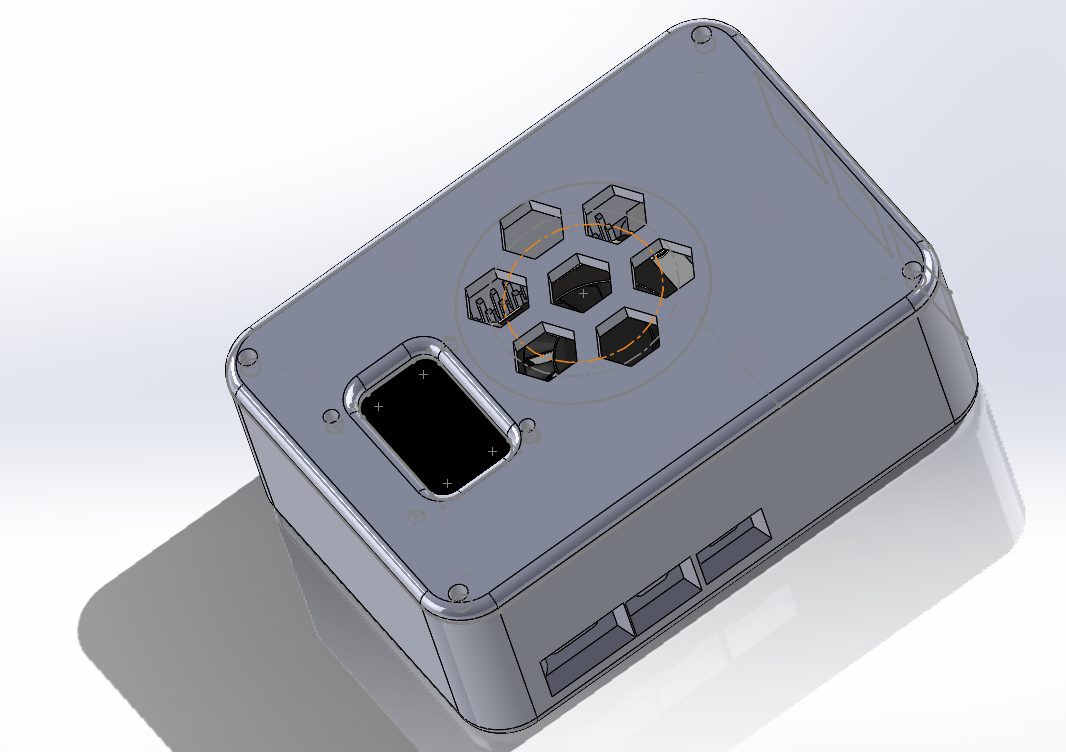
\includegraphics[width=0.85\textwidth]{figures/cad/case_full.png}
    \caption{Vista del conjunto completo de la carcasa de protección diseñada en
    SolidWorks 2022 para el prototipo. \textbf{Fuente:} Elaboración propia.}
    \label{fig:anexo-case-completo}
\end{figure}

\begin{figure}[H]
    \centering
    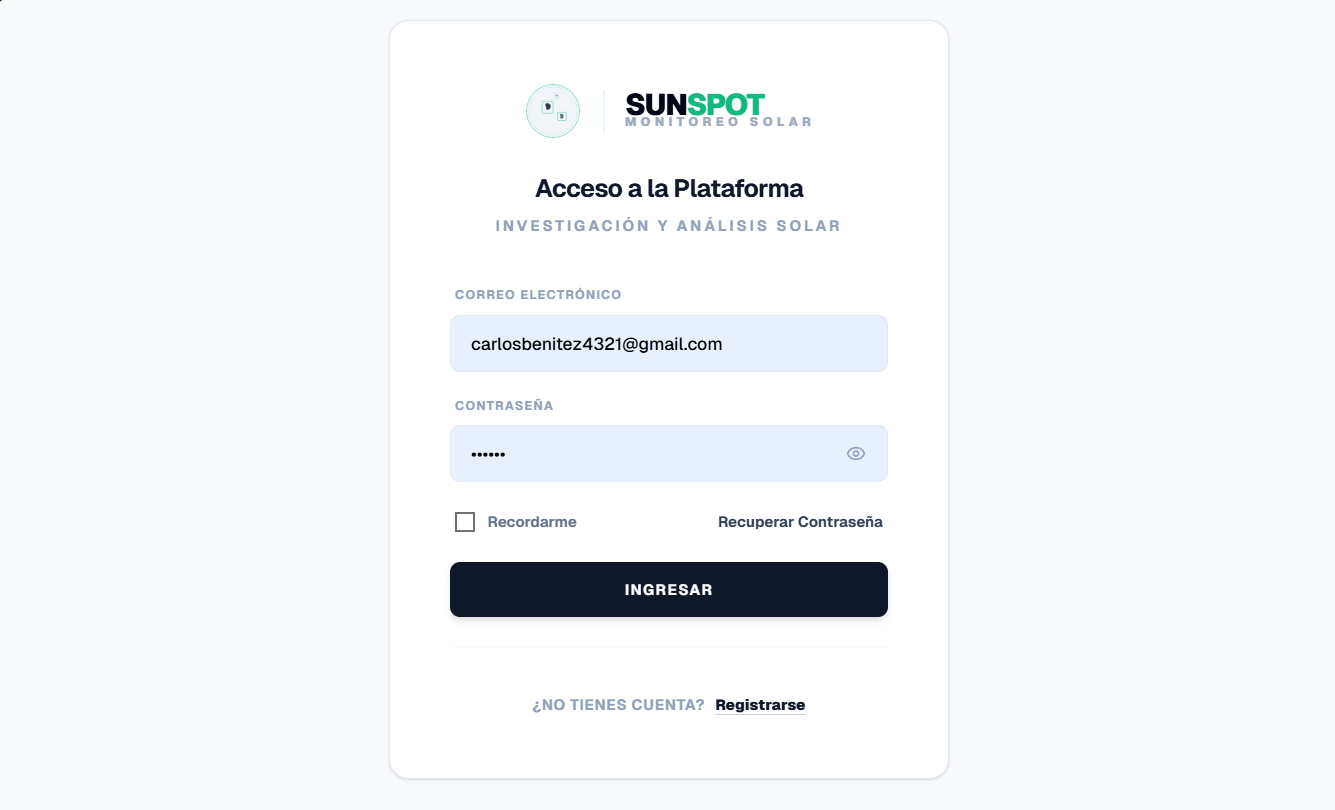
\includegraphics[width=0.95\textwidth]{figures/web/login.png}
    \caption{Pantalla de autenticación de la plataforma web utilizada para
    acceder al entorno de procesamiento y consulta. \textbf{Fuente:} Elaboración propia.}
    \label{fig:anexo-web-login-validacion}
\end{figure}

\begin{figure}[H]
    \centering
    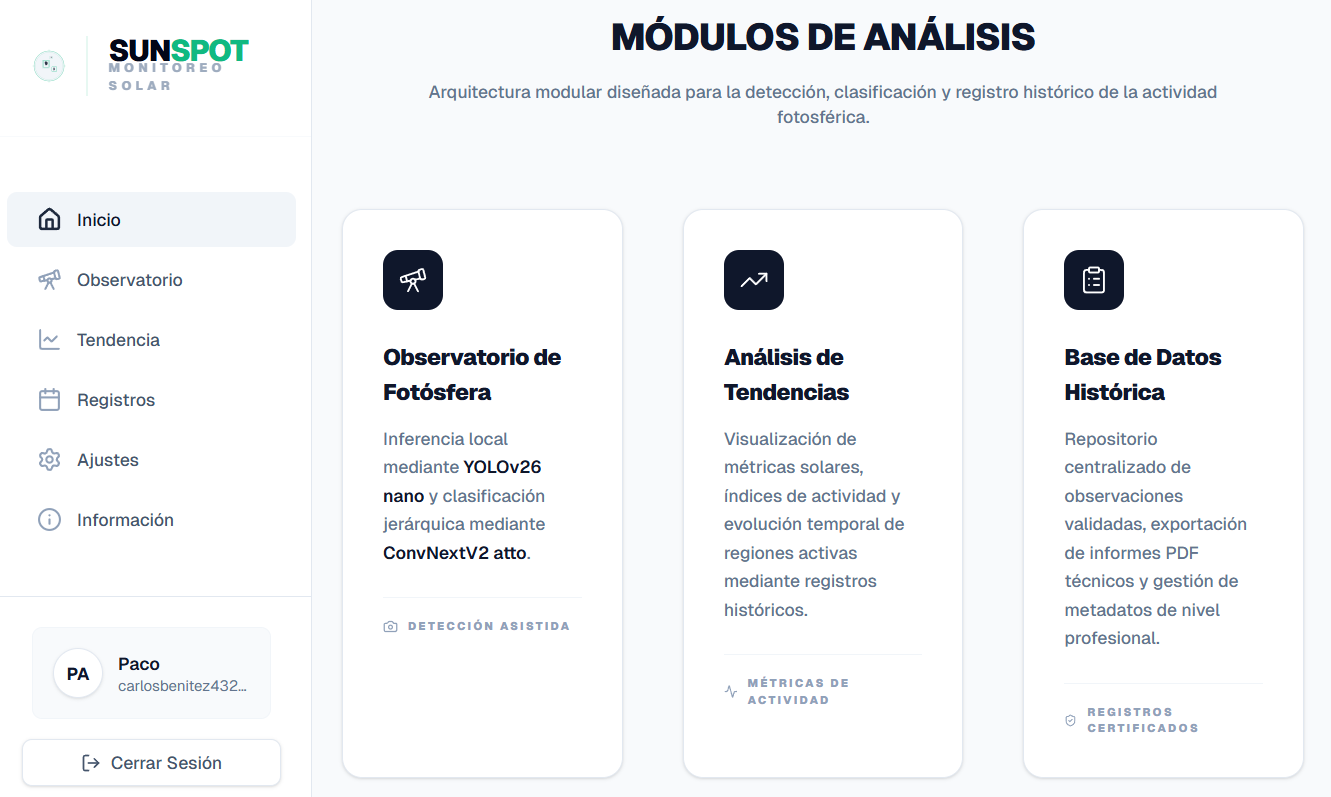
\includegraphics[width=0.95\textwidth]{figures/web/home.png}
    \caption{Vista principal de la plataforma web, desde la cual se organizan
    los módulos de procesamiento, consulta y visualización. \textbf{Fuente:} Elaboración propia.}
    \label{fig:anexo-web-home-validacion}
\end{figure}

\begin{figure}[H]
    \centering
    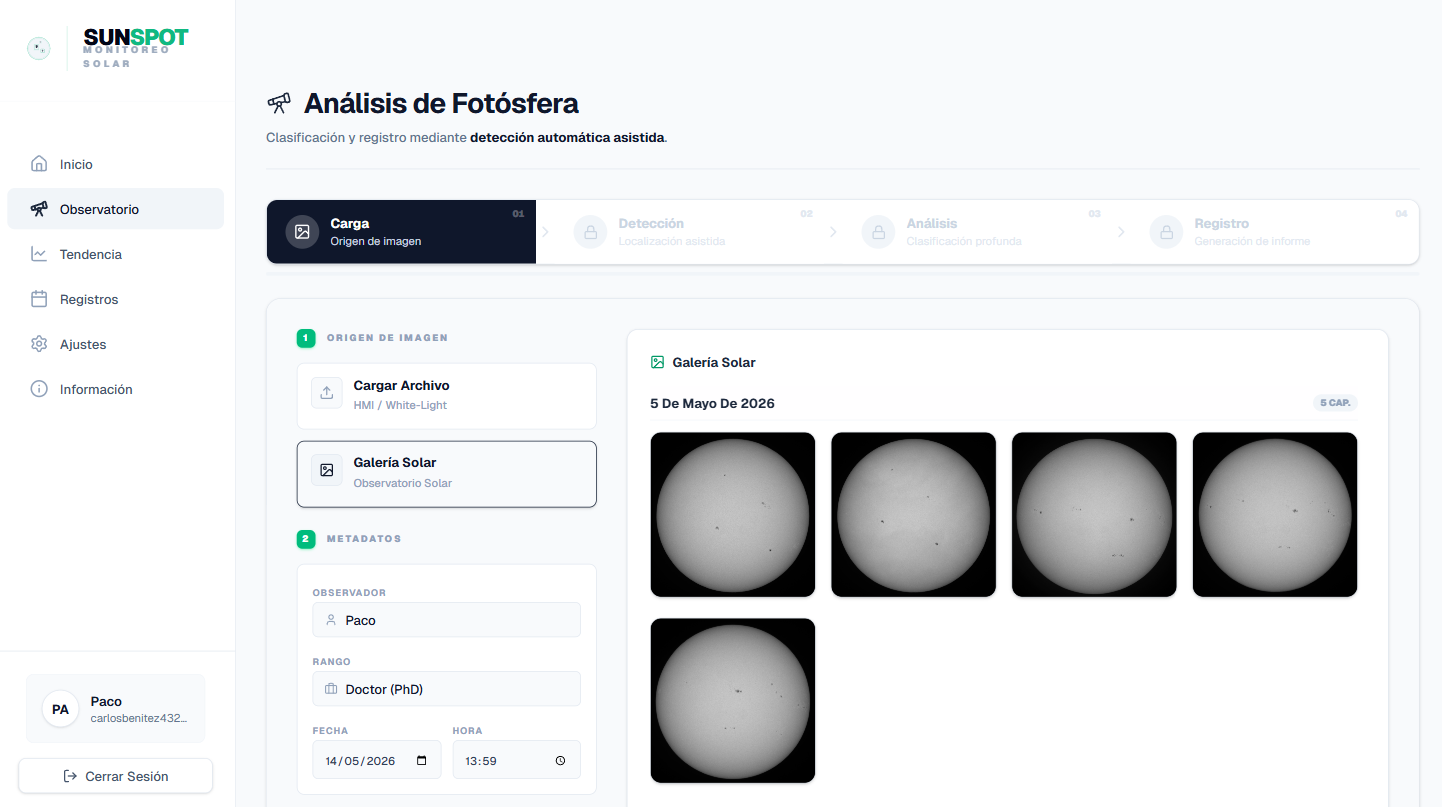
\includegraphics[width=0.95\textwidth]{figures/web/upload.png}
    \caption{Interfaz de carga de imágenes solares para iniciar el flujo de
    procesamiento dentro de la plataforma. \textbf{Fuente:} Elaboración propia.}
    \label{fig:anexo-web-carga-imagen-validacion}
\end{figure}

\end{appendices}
\end{document}
